% Options for packages loaded elsewhere
\PassOptionsToPackage{unicode}{hyperref}
\PassOptionsToPackage{hyphens}{url}
%
\documentclass[
]{book}
\usepackage{lmodern}
\usepackage{amssymb,amsmath}
\usepackage{ifxetex,ifluatex}
\ifnum 0\ifxetex 1\fi\ifluatex 1\fi=0 % if pdftex
  \usepackage[T1]{fontenc}
  \usepackage[utf8]{inputenc}
  \usepackage{textcomp} % provide euro and other symbols
\else % if luatex or xetex
  \usepackage{unicode-math}
  \defaultfontfeatures{Scale=MatchLowercase}
  \defaultfontfeatures[\rmfamily]{Ligatures=TeX,Scale=1}
\fi
% Use upquote if available, for straight quotes in verbatim environments
\IfFileExists{upquote.sty}{\usepackage{upquote}}{}
\IfFileExists{microtype.sty}{% use microtype if available
  \usepackage[]{microtype}
  \UseMicrotypeSet[protrusion]{basicmath} % disable protrusion for tt fonts
}{}
\makeatletter
\@ifundefined{KOMAClassName}{% if non-KOMA class
  \IfFileExists{parskip.sty}{%
    \usepackage{parskip}
  }{% else
    \setlength{\parindent}{0pt}
    \setlength{\parskip}{6pt plus 2pt minus 1pt}}
}{% if KOMA class
  \KOMAoptions{parskip=half}}
\makeatother
\usepackage{xcolor}
\IfFileExists{xurl.sty}{\usepackage{xurl}}{} % add URL line breaks if available
\IfFileExists{bookmark.sty}{\usepackage{bookmark}}{\usepackage{hyperref}}
\hypersetup{
  pdftitle={Knowledge Pool},
  pdfauthor={DAVeMoS team, Institut für Verkehrswesen (IVe), Universität für Bodenkultur Wien},
  hidelinks,
  pdfcreator={LaTeX via pandoc}}
\urlstyle{same} % disable monospaced font for URLs
\usepackage{longtable,booktabs}
% Correct order of tables after \paragraph or \subparagraph
\usepackage{etoolbox}
\makeatletter
\patchcmd\longtable{\par}{\if@noskipsec\mbox{}\fi\par}{}{}
\makeatother
% Allow footnotes in longtable head/foot
\IfFileExists{footnotehyper.sty}{\usepackage{footnotehyper}}{\usepackage{footnote}}
\makesavenoteenv{longtable}
\usepackage{graphicx,grffile}
\makeatletter
\def\maxwidth{\ifdim\Gin@nat@width>\linewidth\linewidth\else\Gin@nat@width\fi}
\def\maxheight{\ifdim\Gin@nat@height>\textheight\textheight\else\Gin@nat@height\fi}
\makeatother
% Scale images if necessary, so that they will not overflow the page
% margins by default, and it is still possible to overwrite the defaults
% using explicit options in \includegraphics[width, height, ...]{}
\setkeys{Gin}{width=\maxwidth,height=\maxheight,keepaspectratio}
% Set default figure placement to htbp
\makeatletter
\def\fps@figure{htbp}
\makeatother
\setlength{\emergencystretch}{3em} % prevent overfull lines
\providecommand{\tightlist}{%
  \setlength{\itemsep}{0pt}\setlength{\parskip}{0pt}}
\setcounter{secnumdepth}{5}
\usepackage{booktabs}
\usepackage{amsthm}
\makeatletter
\def\thm@space@setup{%
  \thm@preskip=8pt plus 2pt minus 4pt
  \thm@postskip=\thm@preskip
}
\makeatother
\usepackage[]{natbib}
\bibliographystyle{apalike}

\title{Knowledge Pool}
\author{DAVeMoS team, Institut für Verkehrswesen (IVe), Universität für Bodenkultur Wien}
\date{2021-12-01}

\begin{document}
\maketitle

{
\setcounter{tocdepth}{1}
\tableofcontents
}
\hypertarget{willkommen}{%
\chapter*{Willkommen}\label{willkommen}}
\addcontentsline{toc}{chapter}{Willkommen}


\includegraphics[width=0.4\linewidth]{image/davemos_logo}

Der Knowledge Pool ist eine sich ständig weiterentwickelnde Datenbank, die Teil des \href{https://www.davemos.online/}{DAVeMoS} Projekts ist. Sie zielt darauf ab, Konzepte und Belege für die systemischen Auswirkungen der Digitalisierung und Automatisierung des Verkehrs zu sammeln. Er ist ein Gemeinschaftswerk der DAVeMoS-Teammitglieder, die mit ihrem Fachwissen, ihren Ideen und Verbesserungsvorschlägen zu Inhalt und Design beigetragen haben:

\begin{itemize}
\tightlist
\item
  Dr.~Msc. MA (Hons) Martyna Bogacz
\item
  B.Sc. Veronika Hebenstreit
\item
  B.Sc. Gregor Husner
\item
  Univ. Prof.~Dr.~Yusak Susilo
\end{itemize}

Die Autoren freuen sich über Feedback, Fragen und Beiträge der Leser. Für weitere Eingaben wenden Sie sich bitte an die korrespondierende Autorin Martyna Bogacz unter der folgenden E-Mail-Adresse: \href{mailto:davemos.library@boku.ac.at}{\nolinkurl{davemos.library@boku.ac.at}}.


\includegraphics[width=0.1\linewidth]{image/cc}
Dieses Werk ist lizenziert unter einer Creative Commons Attribution-NonCommercial-NoDerivatives 4.0 International License.

Die Autoren übernehmen keine Verantwortung oder Haftung für etwaige Fehler oder Unvollständigkeiten im Inhalt dieses Werkes. Die im Knowledge Pool enthaltenen Informationen dienen lediglich der allgemeinen Information.

\textbf{Inhaltsverzeichnis}

\begin{enumerate}
\def\labelenumi{\arabic{enumi}.}
\tightlist
\item
  \protect\hyperlink{intro}{Einleitung}
\item
  \protect\hyperlink{infrastructure}{Physische Straßeninfrastruktur}

  \begin{itemize}
  \tightlist
  \item
    \protect\hyperlink{dedicated_lanes}{Gesonderte Fahrspuren für vernetzte und automatisierte Fahrzeuge (connected and automated vehicles - CAV)}\\
  \item
    \protect\hyperlink{ODD}{Operative Gestaltungsbereiche}\\
  \item
    \protect\hyperlink{rail_crossing_info_system}{Informationssystem für Bahnübergänge}\\
  \item
    \protect\hyperlink{ers}{Elektrisches Straßensystem (Electric road system - ERS)}\\
  \item
    \protect\hyperlink{high_occupancy}{Fahrspuren für Fahrzeuge mit hoher Auslastung (high-occupancy vehicle - HOV)}\\
  \item
    \protect\hyperlink{public_trans_priority}{Prioritätssysteme für den öffentlichen Verkehr}\\
  \item
    \protect\hyperlink{transformation_public_space}{Transformation des öffentlichen Raums und digitale Lösungen}\\
  \end{itemize}
\item
  \protect\hyperlink{highway}{Verwaltung der Straßenverkehrsinfrastruktur}

  \begin{itemize}
  \tightlist
  \item
    \protect\hyperlink{uav}{Unbemannte Luftfahrzeuge für die Instandhaltung der Infrastruktur}\\
  \item
    \protect\hyperlink{charging_station}{Elektrische Ladestationen}\\
  \end{itemize}
\item
  \protect\hyperlink{traffic}{Verkehrsmanagement}

  \begin{itemize}
  \tightlist
  \item
    \protect\hyperlink{congestion_charging}{Staugebühren (Congestion charging)}\\
  \item
    \protect\hyperlink{platooning}{Platooning}\\
  \item
    \protect\hyperlink{traffic_info_monitoring}{Verkehrsinformationen und -überwachung in Echtzeit}\\
  \item
    \protect\hyperlink{cits}{Kooperativ - intelligentes Verkehrssystem (Cooperative - intelligent transport system)}\\
  \item
    \protect\hyperlink{dynamic_route}{Dynamische Routenführung}\\
  \item
    \protect\hyperlink{variable_speed}{Variable Geschwindigkeitsbegrenzungen und dynamisches Beschilderungssystem}\\
  \item
    \protect\hyperlink{adaptive_traffic_control}{Intelligente Verkehrssignalsteuerung}\\
  \item
    \protect\hyperlink{p_g_fleet_management}{Flottenmanagement für Personentransport und Gütertransport}\\
  \item
    \protect\hyperlink{urban_access}{Verwaltung des städtischen Zugangs (Urban Access Management)}\\
  \end{itemize}
\item
  \protect\hyperlink{digital}{Digitale Straßeninfrastruktur und Konnektivität}

  \begin{itemize}
  \tightlist
  \item
    \protect\hyperlink{v2x}{V2X (Vehicle to everything / Fahrzeug-zu-Alles) Kommunikation}\\
  \item
    \protect\hyperlink{infrast_support_level}{Unterstützungsgrad der Infrastruktur für automatisiertes Fahren (ISAD - Infrastructure support for automated driving)}\\
  \end{itemize}
\item
  \protect\hyperlink{passenger}{Fahrgastinformationssystem}

  \begin{itemize}
  \tightlist
  \item
    \protect\hyperlink{djp}{Digitale Fahrplanauskunft}\\
  \item
    \protect\hyperlink{info_and_route_planning}{Multimodale Informationen und Routenplanung}\\
  \end{itemize}
\item
  \protect\hyperlink{multimodal}{Multimodales integriertes System}

  \begin{itemize}
  \tightlist
  \item
    \protect\hyperlink{flms}{Lösungen für die erste und letzte Meile}\\
  \item
    \protect\hyperlink{dist_time_fares}{Fahrpreise für den öffentlichen Personennahverkehr}\\
  \item
    \protect\hyperlink{maas}{Mobilität als Dienstleistung - Mobility as a service (Maas)}\\
  \item
    \protect\hyperlink{p_r}{Park and ride}\\
  \item
    \protect\hyperlink{contactless_cards}{Kontaktlose Karten für öffentliche Verkehrsmittel}\\
  \item
    \protect\hyperlink{special_needs}{Informationen und Unterstützung für Menschen mit besonderen Bedürfnissen}\\
  \item
    \protect\hyperlink{mobility_hubs}{Mobilitätszentren - Mobility hubs}\\
  \item
    \protect\hyperlink{rail_telematics}{Schienenverkehrstelematik für Passagiere und Güterverkehr}\\
  \end{itemize}
\item
  \protect\hyperlink{connected}{Automatisiertes Fahren}

  \begin{itemize}
  \tightlist
  \item
    \protect\hyperlink{av}{Automatisierte PKWs}
  \item
    \protect\hyperlink{parking_av}{Parkinfrastruktur für automatisierte Fahrzeuge}
  \item
    \protect\hyperlink{automated_road_freight}{Automatisierter Straßengüterverkehr}
  \item
    \protect\hyperlink{automatic_train}{Automatischer Zugbetrieb}\\
  \end{itemize}
\item
  \protect\hyperlink{onboard}{Bordtechnologie für vernetzte und automatisierte Fahrzeuge}

  \begin{itemize}
  \tightlist
  \item
    \protect\hyperlink{adas}{Fortschrittliche Fahrerassistenzsysteme (Advanced driver assistance system - ADAS)}\\
  \item
    \protect\hyperlink{parking_assistance}{Einparkhilfe-System}\\
  \item
    \protect\hyperlink{lane_keeping}{Spurhalte-Assistent}\\
  \item
    \protect\hyperlink{digital_maps}{Digitale Landkarten}\\
  \item
    \protect\hyperlink{ehorizon}{Electronic horizon}\\
  \item
    \protect\hyperlink{ecall}{Automatischer Notruf}\\
  \end{itemize}
\item
  \protect\hyperlink{freight}{Güterverkehr und gewerblicher Transport}

  \begin{itemize}
  \tightlist
  \item
    \protect\hyperlink{dangerous_goods}{Lokalisierung und Nachverfolgbarkeit von Waren}\\
  \item
    \protect\hyperlink{intermodal_freight}{Intermodaler Güterverkehr}\\
  \item
    \protect\hyperlink{urban_delivery}{Städtische Lieferungen}\\
  \item
    \protect\hyperlink{intelligent_truck_park}{Intelligentes LKW-Parken}\\
  \item
    \protect\hyperlink{space_book}{Intelligente Lieferflächenbuchung}\\
  \item
    \protect\hyperlink{delivery_drone}{Lieferdrohnen}\\
  \item
    \protect\hyperlink{electric_delivery_fleets}{Elektrofahrzeug-Lieferflotten}\\
  \item
    \protect\hyperlink{mtms}{Multimodale Verkehrsmanagementsysteme}\\
  \item
    \protect\hyperlink{freight_hubs}{Güterverkehrsknotenpunkte}\\
  \end{itemize}
\item
  \protect\hyperlink{collective}{Fahrzeuge der kollektiven Mobilität}

  \begin{itemize}
  \tightlist
  \item
    \protect\hyperlink{drt}{Bedarfsgesteuerte Verkehrssysteme (DRT -- Demand Responsive Transit)}\\
  \item
    \protect\hyperlink{prt}{Personenschnellverkehr (PRT - Personal Rapid Transit)}\\
  \item
    \protect\hyperlink{brt}{Busschnellverkehr (BRT - Bus rapid transit)}\\
  \item
    \protect\hyperlink{lrt}{Stadtbahnverkehr (LRT - Light Rail Transit)}\\
  \end{itemize}
\item
  \protect\hyperlink{big}{Big data}

  \begin{itemize}
  \tightlist
  \item
    \protect\hyperlink{wireless_com}{Drahtlose Kommunikationssysteme}\\
  \item
    \protect\hyperlink{bd_life}{Big data Lebenszyklus}
  \item
    \protect\hyperlink{bd_tool_maping}{Big-Data-Tools für die Kartierung und Vorhersage des Reiseverhaltens}\\
  \end{itemize}
\item
  \protect\hyperlink{shared}{Gemeinschaftliche Mobilität - Shared mobility}

  \begin{itemize}
  \tightlist
  \item
    \protect\hyperlink{car_sharing}{Car sharing}\\
  \item
    \protect\hyperlink{bike_sharing}{(E)-Fahrrad-Sharing}\\
  \item
    \protect\hyperlink{scooters}{E-Kick-Scooter}\\
  \item
    \protect\hyperlink{ride_hailing}{Fahrgemeinschaften (Ride-sharing)}\\
  \item
    \protect\hyperlink{passenger_drones}{Passagierdrohnen}
  \end{itemize}
\item
  \protect\hyperlink{alternative}{Alternative Energieträger}

  \begin{itemize}
  \tightlist
  \item
    \protect\hyperlink{FCEV}{Wasserstoff-Brennstoffzelle}\\
  \item
    \protect\hyperlink{bev}{Batterieelektrisch}\\
  \item
    \protect\hyperlink{plugin_hybrid}{Plugin-Hybridfahrzeuge}\\
  \end{itemize}
\item
  \protect\hyperlink{reference}{Referenzen}
\end{enumerate}

Der Knowledge Pool wurde zusammengestellt am:

\begin{verbatim}
## [1] "01 December 2021"
\end{verbatim}

\hypertarget{inhaltsverzeichnis}{%
\chapter*{Inhaltsverzeichnis}\label{inhaltsverzeichnis}}
\addcontentsline{toc}{chapter}{Inhaltsverzeichnis}

\begin{enumerate}
\def\labelenumi{\arabic{enumi}.}
\tightlist
\item
  \protect\hyperlink{intro}{Einleitung}
\item
  \protect\hyperlink{infrastructure}{Physische Straßeninfrastruktur}

  \begin{itemize}
  \tightlist
  \item
    \protect\hyperlink{dedicated_lanes}{Gesonderte Fahrspuren für vernetzte und automatisierte Fahrzeuge (connected and automated vehicles - CAV)}\\
  \item
    \protect\hyperlink{ODD}{Operative Gestaltungsbereiche}\\
  \item
    \protect\hyperlink{rail_crossing_info_system}{Informationssystem für Bahnübergänge}\\
  \item
    \protect\hyperlink{ers}{Elektrisches Straßensystem (Electric road system - ERS)}\\
  \item
    \protect\hyperlink{high_occupancy}{Fahrspuren für Fahrzeuge mit hoher Auslastung (high-occupancy vehicle - HOV)}\\
  \item
    \protect\hyperlink{public_trans_priority}{Prioritätssysteme für den öffentlichen Verkehr}\\
  \item
    \protect\hyperlink{transformation_public_space}{Transformation des öffentlichen Raums und digitale Lösungen}\\
  \end{itemize}
\item
  \protect\hyperlink{highway}{Verwaltung der Straßenverkehrsinfrastruktur}

  \begin{itemize}
  \tightlist
  \item
    \protect\hyperlink{uav}{Unbemannte Luftfahrzeuge für die Instandhaltung der Infrastruktur}\\
  \item
    \protect\hyperlink{charging_station}{Elektrische Ladestationen}\\
  \end{itemize}
\item
  \protect\hyperlink{traffic}{Verkehrsmanagement}

  \begin{itemize}
  \tightlist
  \item
    \protect\hyperlink{congestion_charging}{Staugebühren (Congestion charging)}\\
  \item
    \protect\hyperlink{platooning}{Platooning}\\
  \item
    \protect\hyperlink{traffic_info_monitoring}{Verkehrsinformationen und -überwachung in Echtzeit}\\
  \item
    \protect\hyperlink{cits}{Kooperativ - intelligentes Verkehrssystem (Cooperative - intelligent transport system)}\\
  \item
    \protect\hyperlink{dynamic_route}{Dynamische Routenführung}\\
  \item
    \protect\hyperlink{variable_speed}{Variable Geschwindigkeitsbegrenzungen und dynamisches Beschilderungssystem}\\
  \item
    \protect\hyperlink{adaptive_traffic_control}{Intelligente Verkehrssignalsteuerung}\\
  \item
    \protect\hyperlink{p_g_fleet_management}{Flottenmanagement für Personentransport und Gütertransport}\\
  \item
    \protect\hyperlink{urban_access}{Verwaltung des städtischen Zugangs (Urban Access Management)}\\
  \end{itemize}
\item
  \protect\hyperlink{digital}{Digitale Straßeninfrastruktur und Konnektivität}

  \begin{itemize}
  \tightlist
  \item
    \protect\hyperlink{v2x}{V2X (Vehicle to everything / Fahrzeug-zu-Alles) Kommunikation}\\
  \item
    \protect\hyperlink{infrast_support_level}{Unterstützungsgrad der Infrastruktur für automatisiertes Fahren (ISAD - Infrastructure support for automated driving)}\\
  \end{itemize}
\item
  \protect\hyperlink{passenger}{Fahrgastinformationssystem}

  \begin{itemize}
  \tightlist
  \item
    \protect\hyperlink{djp}{Digitale Fahrplanauskunft}\\
  \item
    \protect\hyperlink{info_and_route_planning}{Multimodale Informationen und Routenplanung}\\
  \end{itemize}
\item
  \protect\hyperlink{multimodal}{Multimodales integriertes System}

  \begin{itemize}
  \tightlist
  \item
    \protect\hyperlink{flms}{Lösungen für die erste und letzte Meile}\\
  \item
    \protect\hyperlink{dist_time_fares}{Fahrpreise für den öffentlichen Personennahverkehr}\\
  \item
    \protect\hyperlink{maas}{Mobilität als Dienstleistung - Mobility as a service (Maas)}\\
  \item
    \protect\hyperlink{p_r}{Park and ride}\\
  \item
    \protect\hyperlink{contactless_cards}{Kontaktlose Karten für öffentliche Verkehrsmittel}\\
  \item
    \protect\hyperlink{special_needs}{Informationen und Unterstützung für Menschen mit besonderen Bedürfnissen}\\
  \item
    \protect\hyperlink{mobility_hubs}{Mobilitätszentren - Mobility hubs}\\
  \item
    \protect\hyperlink{rail_telematics}{Schienenverkehrstelematik für Passagiere und Güterverkehr}\\
  \end{itemize}
\item
  \protect\hyperlink{connected}{Automatisiertes Fahren}

  \begin{itemize}
  \tightlist
  \item
    \protect\hyperlink{av}{Automatisierte PKWs}
  \item
    \protect\hyperlink{parking_av}{Parkinfrastruktur für automatisierte Fahrzeuge}
  \item
    \protect\hyperlink{automated_road_freight}{Automatisierter Straßengüterverkehr}
  \item
    \protect\hyperlink{automatic_train}{Automatischer Zugbetrieb}\\
  \end{itemize}
\item
  \protect\hyperlink{onboard}{Bordtechnologie für vernetzte und automatisierte Fahrzeuge}

  \begin{itemize}
  \tightlist
  \item
    \protect\hyperlink{adas}{Fortschrittliche Fahrerassistenzsysteme (Advanced driver assistance system - ADAS)}\\
  \item
    \protect\hyperlink{parking_assistance}{Einparkhilfe-System}\\
  \item
    \protect\hyperlink{lane_keeping}{Spurhalte-Assistent}\\
  \item
    \protect\hyperlink{digital_maps}{Digitale Landkarten}\\
  \item
    \protect\hyperlink{ehorizon}{Electronic horizon}\\
  \item
    \protect\hyperlink{ecall}{Automatischer Notruf}\\
  \end{itemize}
\item
  \protect\hyperlink{freight}{Güterverkehr und gewerblicher Transport}

  \begin{itemize}
  \tightlist
  \item
    \protect\hyperlink{dangerous_goods}{Lokalisierung und Nachverfolgbarkeit von Waren}\\
  \item
    \protect\hyperlink{intermodal_freight}{Intermodaler Güterverkehr}\\
  \item
    \protect\hyperlink{urban_delivery}{Städtische Lieferungen}\\
  \item
    \protect\hyperlink{intelligent_truck_park}{Intelligentes LKW-Parken}\\
  \item
    \protect\hyperlink{space_book}{Intelligente Lieferflächenbuchung}\\
  \item
    \protect\hyperlink{delivery_drone}{Lieferdrohnen}\\
  \item
    \protect\hyperlink{electric_delivery_fleets}{Elektrofahrzeug-Lieferflotten}\\
  \item
    \protect\hyperlink{mtms}{Multimodale Verkehrsmanagementsysteme}\\
  \item
    \protect\hyperlink{freight_hubs}{Güterverkehrsknotenpunkte}\\
  \end{itemize}
\item
  \protect\hyperlink{collective}{Fahrzeuge der kollektiven Mobilität}

  \begin{itemize}
  \tightlist
  \item
    \protect\hyperlink{drt}{Bedarfsgesteuerte Verkehrssysteme (DRT -- Demand Responsive Transit)}\\
  \item
    \protect\hyperlink{prt}{Personenschnellverkehr (PRT - Personal Rapid Transit)}\\
  \item
    \protect\hyperlink{brt}{Busschnellverkehr (BRT - Bus rapid transit)}\\
  \item
    \protect\hyperlink{lrt}{Stadtbahnverkehr (LRT - Light Rail Transit)}\\
  \end{itemize}
\item
  \protect\hyperlink{big}{Big data}

  \begin{itemize}
  \tightlist
  \item
    \protect\hyperlink{wireless_com}{Drahtlose Kommunikationssysteme}\\
  \item
    \protect\hyperlink{bd_life}{Big data Lebenszyklus}
  \item
    \protect\hyperlink{bd_tool_maping}{Big-Data-Tools für die Kartierung und Vorhersage des Reiseverhaltens}\\
  \end{itemize}
\item
  \protect\hyperlink{shared}{Gemeinschaftliche Mobilität - Shared mobility}

  \begin{itemize}
  \tightlist
  \item
    \protect\hyperlink{car_sharing}{Car sharing}\\
  \item
    \protect\hyperlink{bike_sharing}{(E)-Fahrrad-Sharing}\\
  \item
    \protect\hyperlink{scooters}{E-Kick-Scooter}\\
  \item
    \protect\hyperlink{ride_hailing}{Fahrgemeinschaften (Ride-sharing)}\\
  \item
    \protect\hyperlink{passenger_drones}{Passagierdrohnen}
  \end{itemize}
\item
  \protect\hyperlink{alternative}{Alternative Energieträger}

  \begin{itemize}
  \tightlist
  \item
    \protect\hyperlink{FCEV}{Wasserstoff-Brennstoffzelle}\\
  \item
    \protect\hyperlink{bev}{Batterieelektrisch}\\
  \item
    \protect\hyperlink{plugin_hybrid}{Plugin-Hybridfahrzeuge}\\
  \end{itemize}
\item
  \protect\hyperlink{reference}{Referenzen}
\end{enumerate}

\hypertarget{intro}{%
\chapter{Einleitung}\label{intro}}

Diese Arbeit sammelt und definiert wesentliche Konzepte im Zusammenhang mit der Automatisierung und Digitalisierung des Verkehrssystems zusammen mit der Beschreibung ihrer Auswirkungen, sowohl negativ als auch positiv auf \textbf{individueller}, \textbf{systemischer} und \textbf{wirtschaftlicher Ebene}. Dieser Knowledge pool wird durch die Tatsache angetrieben, dass Automatisierung und Digitalisierung schnell voranschreiten, wenn auch nicht gleichmäßig in allen Bereichen im Verkehrskontext. Um das Spektrum der Möglichkeiten zu verstehen, die sie mit sich bringen, ist es daher notwendig, die Schlüsselkonzepte zu erklären, ihren Entwicklungsstand und ihre derzeitige Marktdurchdringung aufzuzeigen und schließlich ihre Auswirkungen auf verschiedenen Ebenen zu bewerten. Angesichts dieses Ansatzes enthält jedes Thema die folgenden \textbf{Definition} des Phänomens,
\textbf{Wichtige Interessensgruppen}, die für die jeweilige technologische Entwicklung verantwortlich und von ihr betroffen sind. Dann folgen zwei Unterabschnitte zum \textbf{aktuellen Stand der Forschung und Praxis}. Der erste Abschnitt fasst die neuesten Forschungsergebnisse zu einem bestimmten Thema zusammen, während der zweite Abschnitt den aktuellen Stand der Umsetzung einer bestimmten Technologie in der realen Welt erläutert. Der Abschnitt ``\textbf{Relevante Initiativen in Österreich}'' beschreibt die führenden Initiativen zu einem bestimmten Thema und das Potenzial für österreichische Akteure. Darüber hinaus bieten wir eine zusammenfassende Tabelle über die Auswirkungen des Konzepts auf ausgewählte \textbf{Ziele für nachhaltige Entwicklung} (SDGs). Um ein objektives Maß für den Entwicklungsstand der Technologie in den einzelnen Themenbereichen zu erhalten, haben wir außerdem die sogenannte \textbf{Technology Readiness Scale} (Williamson \& Beasley, 2011) wie unten beschrieben, integriert:

\begin{figure}
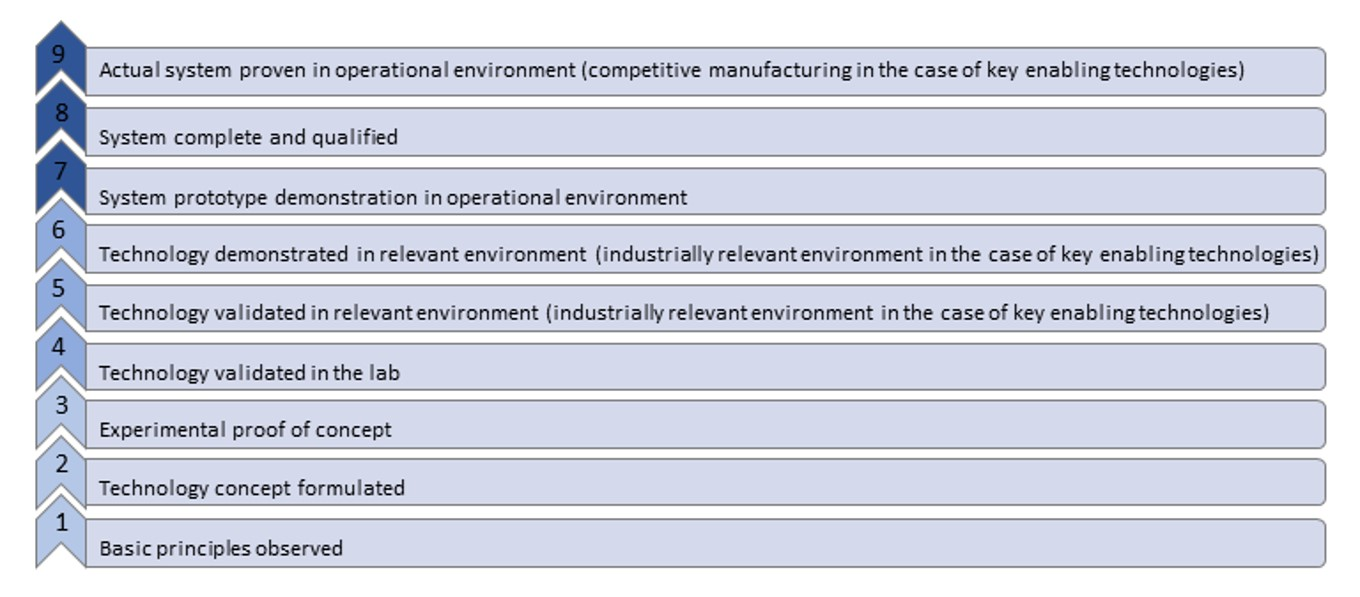
\includegraphics[width=0.8\linewidth]{image/TRL_cropped} \caption{Skala der technologischen Bereitschaft.}\label{fig:unnamed-chunk-4}
\end{figure}

Darüber hinaus bewerten wir die Bereitschaft einer bestimmten Technologie, in der Gesellschaft akzeptiert zu werden, und wie gut sie zum Gemeinwohl beiträgt, indem wir die \textbf{Skala der gesellschaftlichen Bereitschaft} verwenden (McCulloch, 2019):

\begin{figure}
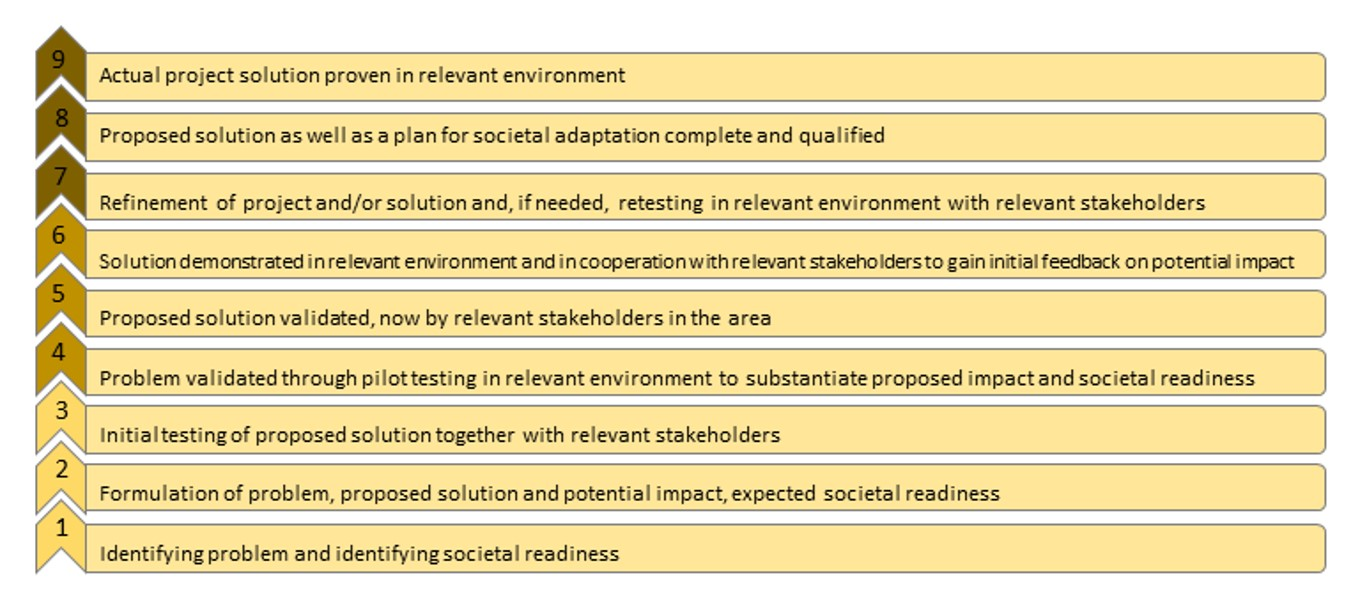
\includegraphics[width=0.8\linewidth]{image/SRL_cropped} \caption{Skala fuer die gesellschaftliche Bereitschaft.}\label{fig:unnamed-chunk-5}
\end{figure}

Abschließend finden Sie eine Liste \textbf{offener Fragen} und \textbf{Links zu weiteren Quellen} zu diesem Thema.

\textbf{Referenzen}

\begin{itemize}
\tightlist
\item
  Williamson, R., \& Beasley, J. (2011). \emph{Automotive technology and manufacturing readiness levels: a guide to recognised stages of development within the automotive industry}. URN11/672.
\item
  McCulloch, S. (2019). Social Acceptance And Societal Readiness Levels. \emph{DecarboN8}. Available at: \url{https://decarbon8.org.uk/social-acceptance-and-societal-readiness-levels/\#:~:text=Societal\%20readiness\%20refers\%20to\%20the,contributes\%20to\%20the\%20public\%20good.} {[}Accessed: 21 January 2021{]}.
\end{itemize}

\hypertarget{infrastructure}{%
\chapter{Physische Straßeninfrastruktur}\label{infrastructure}}

\hypertarget{dedicated_lanes}{%
\section{Gesonderte Fahrspuren für vernetzte und automatisierte Fahrzeuge}\label{dedicated_lanes}}

\hypertarget{synonyme}{%
\subsection*{Synonyme}\label{synonyme}}
\addcontentsline{toc}{subsection}{Synonyme}

\emph{vernetzte und automatisierte Fahrzeuge} \emph{(CAV - connected and automated vehicles)}, \emph{AV-eigene Fahrspuren} \emph{(AV-dedicated lanes)}, \emph{AV-eigene Korridore} \emph{(dedicated corridors)}

\hypertarget{definition}{%
\subsection*{Definition}\label{definition}}
\addcontentsline{toc}{subsection}{Definition}

Dedizierte Fahrspuren für vernetzte und automatisierte Fahrzeuge verfügen über zusätzliche Infrastruktur oder Sensoren, um die Zuverlässigkeit von \protect\hyperlink{adas}{fortschrittlichen Fahrerassistenzsystemen (ADAS)} zu erhöhen. Auf diesen Fahrspuren dürfen nur vollständig automatisiert fahrende Fahrzeuge fahren. Zu den typischen Anwendungen gehören kooperative und adaptive Geschwindigkeitsregelung auf der Grundlage von Sensoren mit der Infrastruktur, Spurhaltung, Optimierung des Kraftstoffverbrauchs und Möglichkeiten der Straßenbenutzung (Broek et al., 2011). Es wird erwartet, dass die Einführung von Sonderfahrspuren für CAV direkte Auswirkungen auf den Verkehrsfluss auf den Autobahnen und im nahen gelegenen Straßennetz haben wird. So zeigte eine in Singapur durchgeführte Studie, dass dedizierte Fahrspuren auf Autobahnen die Fahrzeit von CAVs um etwa 25 \% verkürzen können (wenn die Auslastung der Fahrspur nicht erreicht wird) - auf Kosten einer Verzögerung von etwa 7 \% für konventionelle Fahrzeuge aufgrund der geringeren Kapazität (Ivanchev et al., 2017). Es wurde auch nachgewiesen, dass sie sich positiv auf den Kraftstoffverbrauch auswirken.
Darüber hinaus erhöhte sich der Durchsatz, definiert als Anzahl der Fahrzeuge, die die Straße in einem bestimmten Zeitintervall passieren, infolge der Einführung von speziellen Fahrspuren für AVs (Kumar et al., 2020). Dieser Effekt war jedoch mit einem Rückgang des Durchsatzes auf kleineren Straßen verbunden, da AVs aufgrund der Zeitersparnis Autobahnen bevorzugen, was wiederum zu Zeitverlusten für konventionelle Autos führen kann. Darüber hinaus können die Vorteile einer erhöhten Kapazität von reinen AV-Fahrspuren durch die Festlegung höherer Geschwindigkeitsbegrenzungen für diese Fahrspuren noch verstärkt werden (Ye \& Yamamoto, 2018). In Bezug auf die Nachfrage nach verschiedenen Straßentypen ergab die Studie, dass die Einführung dedizierter AV-Spuren die Nachfrage konventioneller Fahrzeuge nach Hauptverkehrsstraßen (die jedoch kleiner als Autobahnen sind) und Nebenstraßen als Ersatz für stärker überlastete Autobahnen erhöhen wird.
Im Gegensatz dazu hat die Studie von Chen et al.~(2016) gezeigt, dass die Einführung von AV-Spuren das Potenzial hat, die Verkehrskapazität auf diesen Spuren in einem Mischverkehrskontext zu maximieren, während sie praktisch keine Auswirkungen auf die konventionelle Verkehrskapazität hat. Um die dedizierten Fahrspuren für CAVs effizient zu nutzen, die in der Anfangsphase möglicherweise nicht ausreichend ausgelastet sind, wird vorgeschlagen, konventionellen Fahrzeugen die Einfahrt in die reinen Fahrspuren für AVs nach Zahlung der Maut zu ermöglichen. Diese Lösung basiert auf den derzeit weltweit genutzten HOV-Spuren (High Occupancy Vehicle). Es wird behauptet, dass dieser gemeinsame Ansatz den Durchsatz auf einzelnen Straßen und die Verteilung des Verkehrsflusses im gesamten Netz verbessert (Liu \& Song, 2019).

\hypertarget{wichtige-interessensgruppen}{%
\subsection*{Wichtige Interessensgruppen}\label{wichtige-interessensgruppen}}
\addcontentsline{toc}{subsection}{Wichtige Interessensgruppen}

\begin{itemize}
\tightlist
\item
  \textbf{Betroffene}: Fahrer:innen konventioneller Autos, Autohersteller, Versicherungen
\item
  \textbf{Verantwortlich}: Straßeninfrastruktur-Agenturen, lokale und nationale Regierungen
\end{itemize}

\hypertarget{aktueller-stand-der-wissenschaft-und-forschung}{%
\subsection*{Aktueller Stand der Wissenschaft und Forschung}\label{aktueller-stand-der-wissenschaft-und-forschung}}
\addcontentsline{toc}{subsection}{Aktueller Stand der Wissenschaft und Forschung}

Die derzeitige Forschung konzentriert sich darauf, die Auswirkungen der Einführung von Standspuren auf den Verkehrsfluss, die Akzeptanz des Fahrerverhaltens, die Sicherheit und die Effizienz zu ermitteln. Darüber hinaus werden die Faktoren, die diese beeinflussen, analysiert, indem verschiedene Entwurfs- und Betriebskonfigurationen, Straßentypen und Nutzungsstrategien getestet werden (Rad et al., 2020). Es wurden sowohl Feldversuche als auch Studien an Fahrsimulatoren durchgeführt, um den Einfluss verschiedener Designs dedizierter Fahrspuren auf Fahrer:innen in konventionellen Fahrzeugen und solchen mit einem gewissen Grad an Automatisierung zu untersuchen (Guin et al., 2008, Zhong, 2018). Insbesondere wurden in einer Reihe von Studien verschiedene Arten von Fahrspuren verglichen (Zhong, 2018, Yang et al., 2019). Sie zeigten, dass Standspuren mit beschränktem Zugang in Bezug auf Fahrzeit und Durchsatz besser abschnitten als Standspuren mit durchgehendem Zugang. Darüber hinaus war die Wahrscheinlichkeit, dass Fahrzeuge in einem Zug fahren, auf separaten Fahrspuren mit begrenztem Zugang deutlich höher. Andererseits wurde gezeigt, dass die Kollisionsraten in der Nähe der Ein- oder Ausfahrt dieser Fahrspuren mit beschränktem Zugang höher sind (Rad et al.~2020).

\hypertarget{aktueller-stand-der-praktischen-umsetzung}{%
\subsection*{Aktueller Stand der praktischen Umsetzung}\label{aktueller-stand-der-praktischen-umsetzung}}
\addcontentsline{toc}{subsection}{Aktueller Stand der praktischen Umsetzung}

Derzeit plant der Bundesstaat Michigan zusammen mit mehreren privaten Partnern, darunter Ford und Alphabet Inc., 65 km einer Autobahn zwischen Detroit und Ann Arbor für den ausschließlichen Verkehr von vollständig automatisierten Fahrzeugen, einschließlich Bussen und Shuttles, zu reservieren (Krisher \& Eggert, 2020). Ähnliche Initiativen gibt es auch in anderen Ländern. So plant China den Bau einer fast 100 km langen achtspurigen Autobahn zwischen Peking und der Xiongan New Area, von der zwei Fahrspuren für den vollständig automatisierten Verkehr vorgesehen sind. Der Abschluss der Bauphase ist für Ende 2020 vorgesehen, während die Eröffnung für den Verkehr im Juni 2021 erwartet wird (Syncedreview.com, 2020). In Europa läuft derzeit das Projekt SHOW (SHared automation Operating models for Worldwide adoption), das den Einsatz von etwa siebzig vollständig automatisierten Fahrzeugen in 21 europäischen Städten vorsieht. Um zu prüfen, wie sie am besten integriert werden können, werden die Fahrzeuge in verschiedenen Umgebungen im gemischten Verkehr und auf speziellen Fahrspuren eingesetzt. Aus Sicherheitsgründen wird der Fahrer jedoch an Bord sein (CORDIS, 2020).

\hypertarget{relevante-initiativen-in-uxf6sterreich}{%
\subsection*{Relevante Initiativen in Österreich}\label{relevante-initiativen-in-uxf6sterreich}}
\addcontentsline{toc}{subsection}{Relevante Initiativen in Österreich}

\begin{itemize}
\tightlist
\item
  \href{https://www.tugraz.at/fileadmin/user_upload/Institute/IHF/Projekte/ENABLE-S3_SummaryofResults_May2019.pdf}{tugraz.at}
\item
  \href{https://www.ait.ac.at/themen/verkehrssicherheit-und-unfallforschung/projects/via-autonom/}{ait.ac.at}
\end{itemize}

\hypertarget{auswirkungen-in-bezug-auf-die-ziele-fuxfcr-nachhaltige-entwicklung-sdgs}{%
\subsection*{Auswirkungen in Bezug auf die Ziele für nachhaltige Entwicklung (SDGs)}\label{auswirkungen-in-bezug-auf-die-ziele-fuxfcr-nachhaltige-entwicklung-sdgs}}
\addcontentsline{toc}{subsection}{Auswirkungen in Bezug auf die Ziele für nachhaltige Entwicklung (SDGs)}

\begin{longtable}[]{@{}ccccc@{}}
\toprule
\begin{minipage}[b]{0.17\columnwidth}\centering
Ebene der Auswirkungen\strut
\end{minipage} & \begin{minipage}[b]{0.16\columnwidth}\centering
Indikator\strut
\end{minipage} & \begin{minipage}[b]{0.17\columnwidth}\centering
Richtung der Auswirkungen\strut
\end{minipage} & \begin{minipage}[b]{0.17\columnwidth}\centering
Beschreibung des Ziels \& SDG\strut
\end{minipage} & \begin{minipage}[b]{0.17\columnwidth}\centering
Quelle\strut
\end{minipage}\tabularnewline
\midrule
\endhead
\begin{minipage}[t]{0.17\columnwidth}\centering
Individuell\strut
\end{minipage} & \begin{minipage}[t]{0.16\columnwidth}\centering
Geringerer Kraftstoffverbrauch\strut
\end{minipage} & \begin{minipage}[t]{0.17\columnwidth}\centering
\textbf{+}\strut
\end{minipage} & \begin{minipage}[t]{0.17\columnwidth}\centering
Oekologische Nachhaltigkeit (\emph{7,12,13,15})\strut
\end{minipage} & \begin{minipage}[t]{0.17\columnwidth}\centering
Ivanchev et al., 2017\strut
\end{minipage}\tabularnewline
\begin{minipage}[t]{0.17\columnwidth}\centering
Individuell\strut
\end{minipage} & \begin{minipage}[t]{0.16\columnwidth}\centering
Verkuerzte Reisezeit\strut
\end{minipage} & \begin{minipage}[t]{0.17\columnwidth}\centering
\textbf{+}\strut
\end{minipage} & \begin{minipage}[t]{0.17\columnwidth}\centering
Nachhaltige wirtschaftliche Entwicklung (\emph{8,11})\strut
\end{minipage} & \begin{minipage}[t]{0.17\columnwidth}\centering
Zhong, 2018; Yang et al., 2019\strut
\end{minipage}\tabularnewline
\begin{minipage}[t]{0.17\columnwidth}\centering
Systemisch\strut
\end{minipage} & \begin{minipage}[t]{0.16\columnwidth}\centering
Kollisionsrate reduziert\strut
\end{minipage} & \begin{minipage}[t]{0.17\columnwidth}\centering
\textbf{+}\strut
\end{minipage} & \begin{minipage}[t]{0.17\columnwidth}\centering
Gesundheit und Wohlbefinden (\emph{3})\strut
\end{minipage} & \begin{minipage}[t]{0.17\columnwidth}\centering
Zhang et al., 2020\strut
\end{minipage}\tabularnewline
\begin{minipage}[t]{0.17\columnwidth}\centering
Systemisch\strut
\end{minipage} & \begin{minipage}[t]{0.16\columnwidth}\centering
Emissionsrate reduziert\strut
\end{minipage} & \begin{minipage}[t]{0.17\columnwidth}\centering
\textbf{+}\strut
\end{minipage} & \begin{minipage}[t]{0.17\columnwidth}\centering
Oekologische Nachhaltigkeit (\emph{7,12,13,15})\strut
\end{minipage} & \begin{minipage}[t]{0.17\columnwidth}\centering
Al Alam at al., 2010\strut
\end{minipage}\tabularnewline
\begin{minipage}[t]{0.17\columnwidth}\centering
Systemisch\strut
\end{minipage} & \begin{minipage}[t]{0.16\columnwidth}\centering
Verkehrsstaus\strut
\end{minipage} & \begin{minipage}[t]{0.17\columnwidth}\centering
\textbf{\textasciitilde{}}\strut
\end{minipage} & \begin{minipage}[t]{0.17\columnwidth}\centering
Nachhaltige wirtschaftliche Entwicklung (\emph{8,11})\strut
\end{minipage} & \begin{minipage}[t]{0.17\columnwidth}\centering
Ivanchev et al., 2017; Kumar et al., 2020\strut
\end{minipage}\tabularnewline
\begin{minipage}[t]{0.17\columnwidth}\centering
Systemisch\strut
\end{minipage} & \begin{minipage}[t]{0.16\columnwidth}\centering
Neuartige Designs getestet\strut
\end{minipage} & \begin{minipage}[t]{0.17\columnwidth}\centering
\textbf{+}\strut
\end{minipage} & \begin{minipage}[t]{0.17\columnwidth}\centering
Innovation und Infrastruktur (\emph{9})\strut
\end{minipage} & \begin{minipage}[t]{0.17\columnwidth}\centering
Guin et al., 2008; Zhong, 2018; Krisher \& Eggert, 2020\strut
\end{minipage}\tabularnewline
\begin{minipage}[t]{0.17\columnwidth}\centering
Systemisch\strut
\end{minipage} & \begin{minipage}[t]{0.16\columnwidth}\centering
SHOW EU Initiative\strut
\end{minipage} & \begin{minipage}[t]{0.17\columnwidth}\centering
\textbf{+}\strut
\end{minipage} & \begin{minipage}[t]{0.17\columnwidth}\centering
Partnerschaften und Kooperationen (\emph{17})\strut
\end{minipage} & \begin{minipage}[t]{0.17\columnwidth}\centering
CORDIS, 2020\strut
\end{minipage}\tabularnewline
\bottomrule
\end{longtable}

\hypertarget{stand-der-technologischen-und-der-gesellschaftlichen-bereitschaft}{%
\subsection*{Stand der Technologischen und der Gesellschaftlichen Bereitschaft}\label{stand-der-technologischen-und-der-gesellschaftlichen-bereitschaft}}
\addcontentsline{toc}{subsection}{Stand der Technologischen und der Gesellschaftlichen Bereitschaft}

\begin{longtable}[]{@{}cc@{}}
\toprule
Stand der Technologiebereitschaft & Gesellschaftlicher Bereitschaftsgrad\tabularnewline
\midrule
\endhead
5-6 & 1-3\tabularnewline
\bottomrule
\end{longtable}

\hypertarget{offene-fragen}{%
\subsection*{Offene Fragen}\label{offene-fragen}}
\addcontentsline{toc}{subsection}{Offene Fragen}

\begin{enumerate}
\def\labelenumi{\arabic{enumi}.}
\tightlist
\item
  Welches sind die potenziellen Vorteile von dedizierten AV-Spuren in Verbindung mit intelligenten Platooning-Strategien?
\item
  Wie und in welchem Ausmaß werden gemeinsame Konzepte von Automobilsektor, Flotte und Straßenbetreibern das Verkehrsmanagement verbessern und dynamische Verkehrsregelungen auch über Grenzen hinweg?
\item
  Was sind die Rollen und Verantwortlichkeiten der verschiedenen Akteure der physischen Infrastruktur für vernetzte und automatisierte Fahrzeuge?
\item
  Sollte das Fahrzeug mit jeder Straßeninfrastruktur zurechtkommen, und wenn nicht, welche Anforderungen können gestellt werden, um die bestehende Infrastruktur anzupassen?
\item
  Wie kann die Kontinuität zwischen diesen verschiedenen Umgebungen sichergestellt werden?
\item
  Welche Instrumente (z. B. mikro- und makroskopische Verkehrsmodellierung, Folgenabschätzung) können Städte in die Lage versetzen, die Auswirkungen vollständig automatisierter Fahrzeuge auf ihre physische Straßeninfrastruktur zu bewerten und
  die Bedürfnisse der vollständig automatisierten Fahrzeuge mit den Bedürfnissen der bestehenden Verkehrsträger (konventionelle Fahrzeuge, öffentliche Verkehrsmittel, Fußgänger:innen und Radfahrer:innen) abwägen. (ERTRAC, 2019)
\end{enumerate}

\hypertarget{weitere-links}{%
\subsection*{Weitere links}\label{weitere-links}}
\addcontentsline{toc}{subsection}{Weitere links}

\begin{itemize}
\tightlist
\item
  \href{https://knowledge-base.connectedautomateddriving.eu/wp-content/uploads/2019/12/SMART_2010-0064-study-report-final_V1-2.pdf}{knowledge base}
\item
  \href{https://show-project.eu/}{show project}
\end{itemize}

\hypertarget{referenzen}{%
\subsection*{Referenzen}\label{referenzen}}
\addcontentsline{toc}{subsection}{Referenzen}

\begin{itemize}
\tightlist
\item
  Al Alam, A., Gattami, A., \& Johansson, K. H. (2010, September). An experimental study on the fuel reduction potential of heavy duty vehicle platooning. In 13th International IEEE Conference on Intelligent Transportation Systems (pp.~306-311). IEEE.
\item
  Broek, S. M., van Nunen, E., \& Zwijnenberg, H. (2011). Definition of necessary vehicle and infrastructure systems for automated driving.
\item
  Chen, Z., He, F., Zhang, L., \& Yin, Y. (2016). Optimal deployment of autonomous vehicle lanes with endogenous market penetration. Transportation Research Part C: Emerging Technologies, 72, 143-156.
\item
  CORDIS \textbar{} European Commission. (20 Apr 2020). Available at: \url{https://cordis.europa.eu/project/id/875530} {[}Accessed: 13 November 2020{]}.
\item
  ERTRAC Working Group. (2019). Connected Automated Driving Roadmap. version, 8, 2019-08.
\item
  Guin, A., Hunter, M., \& Guensler, R. (2008). Analysis of reduction in effective capacities of high-occupancy vehicle lanes related to traffic behavior. Transportation Research Record, 2065(1), 47-53.
\item
  Ivanchev, J., Knoll, A., Zehe, D., Nair, S., \& Eckhoff, D. (2017). Potentials and implications of dedicated highway lanes for autonomous vehicles. arXiv preprint arXiv:1709.07658.
\item
  Krisher, T., \& Eggert, D. (14 Aug 2020). Michigan plans dedicated road lanes for autonomous vehicles. Available at: \url{https://abcnews.go.com/Technology/wireStory/michigan-plans-dedicated-road-lanes-autonomous-vehicles-72352758} {[}Accessed: 12 November 2020{]}.
\item
  Kumar, A., Guhathakurta, S., \& Venkatachalam, S. (2020). When and where should there be dedicated lanes under mixed traffic of automated and human-driven vehicles for system-level benefits?. Research in Transportation Business \& Management, 100527.
\item
  Liu, Z., \& Song, Z. (2019). Strategic planning of dedicated autonomous vehicle lanes and autonomous vehicle/toll lanes in transportation networks. Transportation Research Part C: Emerging Technologies, 106, 381-403.
\item
  Rad, S. R., Farah, H., Taale, H., van Arem, B., \& Hoogendoorn, S. P. (2020). Design and operation of dedicated lanes for connected and automated vehicles on motorways: A conceptual framework and research agenda. Transportation Research Part C: Emerging Technologies, 117, 102664.
\item
  Syncedreview.com (31 Aug 2020). Beijing Builds 100km Highway Lanes for Self-Driving Cars with Unmanned Machineries. Available at: \url{https://syncedreview.com/2020/08/31/beijing-builds-100km-highway-lanes-for-self-driving-cars-with-unmanned-machineries/} {[}Accessed: 12 November 2020{]}.
\item
  Yang, D., Farah, H., Schoenmakers, M. J., \& Alkim, T. (2019). Human drivers behavioural adaptation when driving next to a platoon of automated vehicles on a dedicated lane and implications on traffic flow: a driving simulator and microscopic simulation study in the Netherlands. In 98th Annual Meeting of the Transportation Research Board (pp.~19-00582).
\item
  Ye, L., \& Yamamoto, T. (2018). Impact of dedicated lanes for connected and autonomous vehicle on traffic flow throughput. Physica A: Statistical Mechanics and its Applications, 512, 588-597.
\item
  Zhang, J., Wu, K., Cheng, M., Yang, M., Cheng, Y., \& Li, S. (2020). Safety Evaluation for Connected and Autonomous Vehicles’ Exclusive Lanes considering Penetrate Ratios and Impact of Trucks Using Surrogate Safety Measures. Journal of advanced transportation, 2020.
\item
  Zhong, Z. (2018). Assessing the effectiveness of managed lane strategies for the rapid deployment of cooperative adaptive cruise control technology.
\end{itemize}

\hypertarget{ODD}{%
\section{Operative Gestaltungsbereiche (Operational design domains)}\label{ODD}}

\hypertarget{synonyme-1}{%
\subsection*{Synonyme}\label{synonyme-1}}
\addcontentsline{toc}{subsection}{Synonyme}

\emph{ODD}

\hypertarget{definition-1}{%
\subsection*{Definition}\label{definition-1}}
\addcontentsline{toc}{subsection}{Definition}

Operational Design Domain (ODD) ist ein System zur Bewertung der Bedingungen, unter denen ein automatisiertes Fahrsystem (automated driving system - ADS) auf der Grundlage von Fahrbahnmerkmalen oder des Verkehrsaufkommens sicher arbeiten kann (Czarnecki, 2018). Es ist ein Schlüssel zur Sicherheit von automatisierten Fahrzeugen, und ODD ist dazu da, die Grenzen für das Fahren auf verschiedenen Automatisierungsstufen eines Fahrzeugs zu definieren (Eliot, 2019). Zum Beispiel hat die Automatisierungsstufe 5 eine uneingeschränkte ODD, was bedeutet, dass sie der Steuerung des Fahrzeugs durch einen menschlichen Fahrer:innen gleichkommt. Bei den Stufen 1-4 unterliegt die ODD Beschränkungen in Bezug auf (Czarnecki, 2018):

\begin{itemize}
\tightlist
\item
  Straßenumgebung: einschließlich, aber nicht beschränkt auf städtische und ländliche Straßen, Autobahnen, Kreisverkehre, Tunnel, Verkehrsaufkommen, Baustellen oder unterschiedliche Wetter- oder Sichtbedingungen
\item
  Zustand des Fahrzeugs: z. B. Beladungsgrenzen oder Mindestfüllstand der Reifen
\item
  Verhalten des mit ADS ausgerüsteten Fahrzeugs: z. B. Geschwindigkeitsbegrenzungen oder Beschränkungen für mögliche Fahrmanöver
\end{itemize}

Im Allgemeinen bewertet ODD die Bedingungen, ob das Fahrzeug in der Lage ist, auf der gewählten Strecke und dem gegebenen Automatisierungsgrad automatisiert zu fahren. Stellt das System irgendwann fest, dass die Bedingungen für automatisiertes Fahren nicht geeignet sind, findet ODD einfach eine Stelle, an der das Fahrzeug angehalten werden kann, und Fahrer:innen müssen selbst das Steuer übernehmen und losfahren.

Der ODD arbeitet auf der Grundlage des operationellen Weltmodells (OWM), das aus dem operationellen Straßenumgebungsmodell \emph{(operational road environment model - OREM)}, dem Modell des betreffenden Fahrzeugs \emph{(subject vehicle(s) model - SVM)} und dem \emph{ADS} besteht. OREM repräsentiert alle relevanten Annahmen über die Straßenumgebung, in der ein ADS betrieben wird, während die irrelevanten ignoriert werden. SVM repräsentiert ein Fahrzeug, das von dem entwickelten ADS betrieben wird. Das OMW kann ein einzelnes Fahrzeug oder mehrere Fahrzeuge umfassen, die mit demselben oder verschiedenen ADS ausgestattet sind. Die Einbeziehung verschiedener ADS kann notwendig sein, um die Interaktion zwischen verschiedenen Fahrzeugtypen wie Bussen und Personenkraftwagen oder denselben Fahrzeugtypen mit unterschiedlichem ADS-Entwicklungsstand darzustellen.

Darüber hinaus führen Koopman und Fratrik (2019) eine Liste von Faktoren an, die für die Validierung und den Betrieb automatisierter Fahrzeuge und folglich für die Entwicklung von ODD als relevant erachtet werden. Dazu gehören:

\begin{itemize}
\tightlist
\item
  Betriebliches Terrain
\item
  Wetterbedingungen
\item
  Betriebliche Infrastruktur
\item
  Einsatzregeln und Interaktion mit der Umgebung und anderen Verkehrsteilnehmer:innen
\item
  Überlegungen zum Einsatz in mehreren Regionen
\item
  Datenverfügbarkeit und Aktualität (z. B. in Bezug auf vorübergehende Änderungen der Verkehrsregeln)
\item
  Erwartete Elemente des operativen Raumzustands (z. B. was sollte in den Anwendungsbereich von ODD einbezogen werden)
\end{itemize}

Darüber hinaus bezieht sich Object and Event Detection and Response (OEDR) auf den Betrieb innerhalb des Geltungsbereichs einer definierten ODD in Bezug auf Objekte und Ereignisse. Zu den \emph{Objektfaktoren} gehören:

\begin{itemize}
\tightlist
\item
  Fähigkeit, relevante Objekte in der Umgebung zu erkennen und zu klassifizieren
\item
  Verarbeitung und Schwellenwertbildung von Sensordaten
\item
  Charakterisierung möglicher Betriebsparameter anderer Verkehrsteilnehmer:innen
\item
  Permanente (Bäume, Bordsteine usw.) und temporäre (z. B. Menschen, Überschwemmungen) Hindernisse
\item
  Gefährdete Bevölkerung
\item
  Alle Arten von anderen Verkehrsteilnehmer:innen, einschließlich von Menschen gesteuerter und automatisierter Fahrzeuge sowie von Spezialfahrzeugen und Flugzeugen
\end{itemize}

Darüber hinaus beziehen sich die \emph{Ereignisfaktoren} auf:
- Bestimmung des Verhaltens anderer Objekte
- `Normale' Bewegung von Objekten
- `Anormale' Bewegung von Objekten
- Ausbleiben der Bewegung anderer Objekte
- Interaktionen des/der Fahrer:in vor, während und nach dem Einsatz des automatisierten Systems
- Menschliche und nicht-menschliche Interaktionen

\hypertarget{wichtige-interessensgruppen-1}{%
\subsection*{Wichtige Interessensgruppen}\label{wichtige-interessensgruppen-1}}
\addcontentsline{toc}{subsection}{Wichtige Interessensgruppen}

\begin{itemize}
\tightlist
\item
  \textbf{Betroffene}: Fahrer:innen konventioneller Autos, Autohersteller, Nutzer:innen von AVs
\item
  \textbf{Verantwortlich}: Stadtverwaltungen, Autohersteller, Versicherungsanbieter
\end{itemize}

\hypertarget{aktueller-stand-der-wissenschaft-und-forschung-1}{%
\subsection*{Aktueller Stand der Wissenschaft und Forschung}\label{aktueller-stand-der-wissenschaft-und-forschung-1}}
\addcontentsline{toc}{subsection}{Aktueller Stand der Wissenschaft und Forschung}

Die aktuelle Forschung konzentriert sich auf die Validierung, die Erweiterung der Fähigkeiten und die Verbesserung der Genauigkeit der derzeitigen ODD-Systeme. Lee et al.~(2020) schlagen beispielsweise einen Ansatz zur Ermittlung einer ODD für das ADS anhand von statistischen Daten und Risikotoleranz vor. Die ermittelte ODD basiert auf der geografischen Zuordnung des mit dem ADS-Betrieb verbundenen Risikoniveaus, das unter der für eine bestimmte Umweltbedingung vordefinierten Risikoschwelle liegt. Daher ermöglicht diese Methode die Berücksichtigung von Sicherheitsbedenken durch die Festlegung von geografischen und umweltbedingten Einschränkungen für den ADS-Betrieb. Darüber hinaus untersuchten Farah et al.~(2020) das Verständnis von ODD (in Bezug auf das Halten der Fahrspur) durch menschliche Fahrer:innen, von denen erwartet wird, dass sie das Fahrzeug in Situationen außerhalb der vom Hersteller angegebenen ODD steuern. Ein Unterschied zwischen dem Verständnis der Fahrer:innen für die Fähigkeiten des AV und dem Handbuch des Herstellers kann zu ernsthaften Sicherheitsproblemen führen. Sie führten einen Feldtest mit einem Tesla Model S durch, der auf Situationen innerhalb und außerhalb der vom Hersteller angegebenen ODD basierte. Farah et al.~(2020) fanden eine Diskrepanz zwischen der vom Hersteller angegebenen ODD und der Wahrnehmung der Fahrer:innen, was die ODD umfasst. Insbesondere wurden Situationen, die außerhalb des Geltungsbereichs der ODD lagen, von menschlichen Fahrer:innen häufig als innerhalb des ODD-Bereichs liegend eingestuft. Diese Studie hat gezeigt, dass die ODD klarer beschrieben und spezifiziert werden muss, um die Diskrepanz zwischen dem Bewusstsein der Fahrer:innen und den tatsächlichen Fähigkeiten des Fahrzeugs zu verringern.

\hypertarget{aktueller-stand-der-praktischen-umsetzung-1}{%
\subsection*{Aktueller Stand der praktischen Umsetzung}\label{aktueller-stand-der-praktischen-umsetzung-1}}
\addcontentsline{toc}{subsection}{Aktueller Stand der praktischen Umsetzung}

Kalifornien ist einer der Pionierstaaten, die Versuche zur Erprobung von ODD durchführen. Eines der Beispiele ist das aktuelle Google-Projekt des fahrerlosen Testwagens von Waymo \href{https://www.losaltoshills.ca.gov/DocumentCenter/View/2315/Waymo_Driverless_Autonomous_Vehicle_Tester_Program}{Waymo’s}. Es verwendet eine vierte Stufe des automatisierten Fahrsystems und zeigt die Verwendung von ODD im wirklichen Leben. Das ODD von Waymo arbeitet in einem bestimmten geografischen Gebiet (einem Teil Kaliforniens) 24 Stunden am Tag. Waymos ODD kann bis zu 105 km/h erreichen, funktioniert aber nicht bei Schnee oder Regen. Ansonsten gibt es in den USA keine landesweite Regelung für den Einsatz von ODD, da diese sehr ortsabhängig sind. Andere Regionen der Welt arbeiten an eigenen Regelungen für ODDs, wie z. B. MLIT-Guidline in Japan, Transport Canada in Kanada, NHTSA FAVP 3.0 in den USA oder EG-Richtlinien in Europa. Darüber hinaus hat die informelle Arbeitsgruppe der Vereinten Nationen für funktionale Anforderungen für AVs (FRAV) einen {[}Bericht{]} (\url{https://unece.org/fileadmin/DAM/trans/doc/2020/wp29grva/GRVA-05-40e.pdf}) zur Regelung der funktionalen Leistungsanforderungen für automatisierte Fahrsysteme und mit solchen Systemen ausgestattete Fahrzeuge vorgelegt.

\hypertarget{relevante-initiativen-in-uxf6sterreich-1}{%
\subsection*{Relevante Initiativen in Österreich}\label{relevante-initiativen-in-uxf6sterreich-1}}
\addcontentsline{toc}{subsection}{Relevante Initiativen in Österreich}

\begin{itemize}
\tightlist
\item
  \href{https://austriatech.at/de/das-konzept-der-isad-klassen/}{AustriaTech}
\end{itemize}

\hypertarget{auswirkungen-in-bezug-auf-die-ziele-fuxfcr-nachhaltige-entwicklung-sdgs-1}{%
\subsection*{Auswirkungen in Bezug auf die Ziele für nachhaltige Entwicklung (SDGs}\label{auswirkungen-in-bezug-auf-die-ziele-fuxfcr-nachhaltige-entwicklung-sdgs-1}}
\addcontentsline{toc}{subsection}{Auswirkungen in Bezug auf die Ziele für nachhaltige Entwicklung (SDGs}

\begin{longtable}[]{@{}ccccc@{}}
\toprule
\begin{minipage}[b]{0.17\columnwidth}\centering
Ebene der Auswirkungen\strut
\end{minipage} & \begin{minipage}[b]{0.16\columnwidth}\centering
Indikator\strut
\end{minipage} & \begin{minipage}[b]{0.17\columnwidth}\centering
Richtung der Auswirkungen\strut
\end{minipage} & \begin{minipage}[b]{0.17\columnwidth}\centering
Beschreibung des Ziels \& SDG\strut
\end{minipage} & \begin{minipage}[b]{0.17\columnwidth}\centering
Quelle\strut
\end{minipage}\tabularnewline
\midrule
\endhead
\begin{minipage}[t]{0.17\columnwidth}\centering
Systemisch\strut
\end{minipage} & \begin{minipage}[t]{0.16\columnwidth}\centering
Mehr Sicherheit fuer automatisierte Fahrzeuge angestrebt\strut
\end{minipage} & \begin{minipage}[t]{0.17\columnwidth}\centering
\textbf{+}\strut
\end{minipage} & \begin{minipage}[t]{0.17\columnwidth}\centering
Gesundheit und Wohlbefinden (\emph{3})\strut
\end{minipage} & \begin{minipage}[t]{0.17\columnwidth}\centering
Koopman and Fratrik, 2019\strut
\end{minipage}\tabularnewline
\begin{minipage}[t]{0.17\columnwidth}\centering
Systemisch\strut
\end{minipage} & \begin{minipage}[t]{0.16\columnwidth}\centering
Entwicklung vollstaendig automatisierter Autos\strut
\end{minipage} & \begin{minipage}[t]{0.17\columnwidth}\centering
\textbf{+}\strut
\end{minipage} & \begin{minipage}[t]{0.17\columnwidth}\centering
Innovation und Infrastruktur (\emph{9})\strut
\end{minipage} & \begin{minipage}[t]{0.17\columnwidth}\centering
Waymo, 2019\strut
\end{minipage}\tabularnewline
\bottomrule
\end{longtable}

\hypertarget{stand-der-technologiebereitschaft-und-gesellschaftlicher-bereitschaftsgrad}{%
\subsection*{Stand der Technologiebereitschaft und Gesellschaftlicher Bereitschaftsgrad}\label{stand-der-technologiebereitschaft-und-gesellschaftlicher-bereitschaftsgrad}}
\addcontentsline{toc}{subsection}{Stand der Technologiebereitschaft und Gesellschaftlicher Bereitschaftsgrad}

\begin{longtable}[]{@{}cc@{}}
\toprule
TRL & SRL\tabularnewline
\midrule
\endhead
5-6 & 4-6\tabularnewline
\bottomrule
\end{longtable}

\hypertarget{offene-fragen-1}{%
\subsection*{Offene Fragen}\label{offene-fragen-1}}
\addcontentsline{toc}{subsection}{Offene Fragen}

\begin{enumerate}
\def\labelenumi{\arabic{enumi}.}
\tightlist
\item
  Welchen Einfluss hat die Entwicklung von ODD auf den Markt für automatisierte Fahrzeuge für den Durchschnittsfahrer?
\end{enumerate}

\hypertarget{referenzen-1}{%
\subsection*{Referenzen}\label{referenzen-1}}
\addcontentsline{toc}{subsection}{Referenzen}

\begin{itemize}
\tightlist
\item
  Berman, B., 2019. Autonomous vehicle operation design domain is key to safety. Sae.org. Available at: \url{https://www.sae.org/news/2019/11/odds-for-av-testing} {[}Accessed: 2 August 2021{]}.
\item
  Czarnecki, K. (2018). Operational Design Domain for Automated Driving Systems - Taxonomy of Basic Terms. 10.13140/RG.2.2.18037.88803.
\item
  Eliot, L., 2019. Key To Driverless Cars, Operational Design Domains (ODD), Here’s What They Are, Woes Too. Medium. Available at: \url{https://lance-eliot.medium.com/key-to-driverless-cars-operational-design-domains-odd-heres-what-they-are-woes-too-a0f1059e0bdb} {[}Accessed: 2 August 2021{]}.
\item
  Farah, H., Bhusari, S., Van Gent, P., Babu, F. A. M., Morsink, P., Happee, R., \& van Arem, B. (2020). An empirical analysis to assess the operational design domain of lane keeping system equipped vehicles combining objective and subjective risk measures. IEEE Transactions on Intelligent Transportation Systems, 22(5), 2589-2598.
\item
  Koopman, P. and Fratrik, F., (2019). How Many Operational Design Domains, Objects, and Events?. Ceur-ws.org. Available at: \url{http://ceur-ws.org/Vol-2301/paper_6.pdf} {[}Accessed: 2 August 2021{]}.
\item
  Law Insider. (2021). Operational design domain Definition \textbar{} Law Insider. Available at: \url{https://www.lawinsider.com/dictionary/operational-design-domain} {[}Accessed: 2 August 2021{]}.
\item
  Lee, C., Nayeer, N., Garcia, D., Agrawal, A. and Liu, B., 2020. Identifying the Operational Design Domain for an Automated Driving System through Assessed Risk. 2020 IEEE Intelligent Vehicles Symposium (IV).
\item
  Waymo. 2019. Waymo. Available at: \url{https://waymo.com/} {[}Accessed: 2 August 2021{]}.
\end{itemize}

\hypertarget{rail_crossing_info_system}{%
\section{Informationssystem für Bahnübergänge}\label{rail_crossing_info_system}}

\hypertarget{synonyme-2}{%
\subsection*{Synonyme}\label{synonyme-2}}
\addcontentsline{toc}{subsection}{Synonyme}

\emph{Bahnübergänge (rail level crossings - RLX), erhöhte Bahnübergänge (raised level crossings - RC), Bahnübergangshinderniserkennung (Level Crossing Obstacle Detection - LOD), Bahnübergang (level crossing - LC)}

\hypertarget{definition-2}{%
\subsection*{Definition}\label{definition-2}}
\addcontentsline{toc}{subsection}{Definition}

Ein anhaltendes Problem im Landverkehr sind Kollisionen an Bahnübergängen (RLX). RLX sind höhengetrennte Kreuzungen, an denen Schienenfahrzeuge (und ihre Infrastruktur) die Infrastruktur eines anderen Verkehrsträgers (in der Regel Straßen) kreuzen. In den meisten Fällen hat der Zug Vorrang und der übrige Verkehr wird angehalten, bis der Zug vorbeigefahren ist. Technisch gesehen ist diese Entflechtung ein einfaches Problem (Salmon et al., 2016). Dennoch kommt es jedes Jahr zu einer Reihe von Unfällen.
Kollisionen an Bahnübergängen stellen weltweit ein Sicherheitsrisiko dar (European Railway Agency, 2020). Unfälle verursachen menschliche, soziale und wirtschaftliche Kosten. Darüber hinaus wirken sich Beinahe-Kollisionen negativ auf die psychische Gesundheit und das Wohlbefinden der beteiligten Personen -- Autofahrer:innen, Zugführer:innen und Umstehende - aus (Read et al., 2021). Die beste Möglichkeit, diese Art von Unfällen zu minimieren, wäre die Beseitigung der Bahnübergänge und/oder deren Ersatz durch Tunnel oder Brücken. Da diese Optionen sehr kostspielig sind, wird für die meisten Bahnübergänge die billigere Alternative von Schildern, Blinklichtern und Schranken verwendet, in der Erwartung, dass sich die Fahrer:innen von Straßenfahrzeugen an die Regeln halten werden. Daten aus Australien zeigen jedoch, dass der größte Teil der Kollisionen an Kreuzungen mit Schranken stattfindet, während der größte Teil der tödlichen Unfälle an Kreuzungen mit Blinklicht und Stoppschildern passiert (ITSR, 2011).
Radalj et al.~(2011) haben in einer umfangreichen Feldstudie in sieben ländlichen Gemeinden nachgewiesen, dass 90 \% der Verkehrsteilnehmer:innen die Geschwindigkeitsbegrenzungen an den Signalen missachteten und dass 90 \% der Unfälle an Bahnübergängen auf Fehler der Fahrzeugführer:innen, Müdigkeit, Geschwindigkeit oder Risikobereitschaft aufgrund der geringen Zugfrequenz zurückzuführen waren. Auch in Österreich gibt es bereits Daten, die zeigen, dass praktisch alle Unfälle an Bahnübergängen von Verkehrsteilnehmer:innenn verursacht werden, die rote Ampeln, Stoppschilder, Schranken und grundlegende Verkehrsregeln nicht beachten. Sehr oft sind Menschen, die in der Nähe eines Bahnübergangs wohnen oder ihn regelmäßig überqueren, in diese Unfälle verwickelt, weil sie mit der Zeit unvorsichtiger und übermütiger werden (bmvit, 2011).
Gemäß der Europäischen Union (2014) werden Bahnübergänge in aktive und passive unterteilt:

\begin{itemize}
\tightlist
\item
  \textbf{Ein passiver Bahnübergang } ist ein Bahnübergang ohne jede Form von Warnsystem oder Schutz, der aktiviert wird, wenn es für Benutzer:innen unsicher ist, ihn zu überqueren.
\item
  \textbf{Ein aktiver Bahnübergang } ist ein Bahnübergang, bei dem die Benutzer:innen des Bahnübergangs vor einem herannahenden Zug geschützt oder gewarnt werden. Der Schutz wird durch Halb- oder Vollschranken gewährleistet. Die Warnung erfolgt durch sichtbare (z. B. Lichter) und akustische Vorrichtungen (z. B. Glocken, Hupen, Schallsignale).
\end{itemize}

Aktive Bahnübergänge werden klassifiziert als:
- \textbf{Manuell}: ein Bahnübergang, bei dem die benutzerseitige Sicherung oder Warnung manuell von Bahnmitarbeiter:innen aktiviert wird.
- \textbf{Automatisch mit benutzerseitiger Warnung: }: Ein Bahnübergang, bei dem die benutzerseitige Warnung durch den herannahenden Zug aktiviert wird.
- \textbf{Automatisch mit benutzerseitigem Schutz}: Ein Bahnübergang, bei dem der benutzerseitige Schutz durch den herannahenden Zug aktiviert wird. Dazu gehört auch ein Bahnübergang, der sowohl über einen benutzerseitigen Schutz als auch über eine Warnung verfügt.
- \textbf{Gleisseitiger Schutz}: Ein Bahnübergang, bei dem ein Signal oder ein anderes Zugsicherungssystem die Weiterfahrt eines Zuges nur dann zulässt, wenn der Bahnübergang frei von Hindernissen ist.

Die streckenseitige Sicherung ermöglicht die Erkennung von Hindernissen an Bahnübergängen durch eine oder mehrere Erfassungseinheiten, je nach Größe des Bahnübergangs. Eine streckenseitige Steuereinheit sammelt die von den Erfassungseinheiten empfangenen Informationen und erzeugt Alarme auf der Grundlage hoher Schwellenwerte (z. B. Mindestabmessungen des Hindernisses). Die Steuereinheit ist in der Lage, die Bahnübergangshinderniserkennung (BÜH) in die konventionelle Bahnübergangssicherung mit kompletten Schranken und Antrieben zu integrieren und über gesicherte Schnittstellen mit dem Stellwerk zu kommunizieren. Die Systeme zeichnen sich durch hohe Zuverlässigkeit und hohe Genauigkeit aus, auch bei rauen Wetterbedingungen wie Regen, Schnee und Nebel. Derzeit laufen mehrere Versuche mit europäischen Bahnen (mermecgroup, n.d.).

Laut Darlington (2017) muss ein ideales Hinderniserkennungssystem:

\begin{itemize}
\tightlist
\item
  eine Sicherheitsintegrität bieten, die nicht schlechter und idealerweise besser ist als bei einem manuell betriebenen Bahnübergang
\item
  keine oder nur minimale Verspätungen von Zügen aufgrund von Geräteausfällen oder Fehldetektionen verursachen
\item
  in Bezug auf die Lebenszykluskosten erschwinglich sein
\item
  bei allen Wetterbedingungen und Temperaturen funktionieren
\item
  praktisch zu bedienen und zu warten sein
\end{itemize}

Darüber hinaus müssen getrennte technische Systeme bestätigen, dass der Bahnübergang durch Schranken oder Tore geschlossen ist, und erst wenn das Detektionssystem bestätigt hat, dass der Bahnübergang frei ist, wird der Zug durchgelassen. Dies könnte durch die Freigabe der Schutzsignale oder, auf einigen Schienennetzen, durch eine direkte Kommunikationsverbindung zum Zug erreicht werden. Einige Systeme bieten zwar gute Sicherheitsvorteile, aber nur auf Kosten erheblicher betrieblicher Verzögerungen. Das Hinderniserkennungssystem muss sich in die bestehende Eisenbahninfrastruktur einfügen und soll den Betrieb nicht beeinträchtigen.
Für die Hinderniserkennung stehen folgende Technologien zur Verfügung, die jedoch alle Vor- und Nachteile haben (Darlington, 2017):

\textbf{Videobildtechnik}
Der Nachteil der Videotechnik besteht darin, dass das System bei Nacht oder Nebel nur schwer etwas erkennen kann. Der Bahnübergang benötigt daher möglicherweise die gleiche oder eine höhere Beleuchtungsstärke als ein manueller Bahnübergang, obwohl dies bei Nebel wenig hilfreich wäre. Außerdem lassen sich die Masse oder die Materialeigenschaften eines Objekts nicht so leicht unterscheiden. So könnte beispielsweise ein Karton oder eine Zeitung fälschlicherweise für ein kleines Kind gehalten werden.

\textbf{Wärmebildtechnik}
Wärmebildkameras können einige dieser Einschränkungen überwinden, da sie auf der Grundlage feiner Temperaturunterschiede ein scharfes Bild erzeugen und nicht durch Umgebungsbedingungen wie völlige Dunkelheit, Rauch oder Nebel beeinträchtigt werden. Sie benötigen kein Licht und können nicht durch direktes Sonnenlicht geblendet werden. Allerdings könnten Objekte ohne Wärmequelle an einer Kreuzung zurückgelassen werden (z. B. ein ungebremster Anhänger) und somit nicht erkannt werden. Die Wärmebildtechnik kann in Kombination mit anderen Erkennungstechnologien eine Lösung bieten.

\textbf{Strahlunterbrechung im Millimeterwellenbereich}
Die Strahlunterbrechung ist eine auf Mikrowellen basierende Technik zur Hinderniserkennung. Wenn ein Objekt in den Strahlengang eindringt, wird das Signal zum Sende-Empfangsgerät abgeschwächt, was die Anwesenheit des Objekts anzeigt. Eines der weltweit ersten Systeme der Sicherheitsintegritätsstufe (SIL) 4 wurde in Italien installiert. Obwohl das System sicher war, reagierte es sehr empfindlich auf Temperaturschwankungen, Regen und Kondenswasser auf den Sensoren von Sender und Empfänger. Es musste regelmäßig kalibriert und gewartet werden. Außerdem bedeuteten die geringe Strahlbreite und das begrenzte Sichtfeld, dass für hohe Objekte noch mehr Sensoren benötigt wurden.

\textbf{LiDAR}
LiDAR erfasst den Kreuzungsbereich mit Impulsen aus Nahinfrarotlicht, die von der Oberfläche eines Objekts auf dem Bahnübergang reflektiert werden. Die reflektierten Impulse können dann analysiert werden, um seine Position, Richtung und Geschwindigkeit zu bestimmen. Da Licht eine kürzere Wellenlänge als Radiowellen hat, bietet LiDAR das Potenzial für eine höhere Genauigkeit als Radar. Network Rail hat LiDAR bei seiner ersten Generation von OD-Kreuzungen als Ergänzung zum Radar eingesetzt, um die Erkennung von Objekten in niedriger Höhe zu verbessern. Die verbesserte Empfindlichkeit bedeutet jedoch auch, dass das System anfällig für kleine Objekte ist, wie z. B. Wasserdampftröpfchen, aus denen sich Nebel zusammensetzt, obwohl dies durch Softwarealgorithmen abgemildert werden kann. Außerdem wird für den Betrieb Licht benötigt, und die Geräte müssen in einem transparenten Gehäuse untergebracht werden, was zu einer erhöhten Anfälligkeit für Wasser, Schmutz und Staub auf dem Glas führt.

\textbf{Induktionsschleifen}
Eine Induktionsschleife wird zur Erkennung von Metallobjekten verwendet und eignet sich daher nicht für die Erkennung von Fußgänger:innen. Leider gibt es immer mehr Straßenfahrzeuge aus Verbundwerkstoffen und Aluminium, die einen geringeren induzierten Strom liefern als Stahl, und es wurde über Probleme bei der Erkennung von Lastwagen mit hohen Achsen/Bodenfreiheit berichtet. Eine weitere Schwierigkeit ist die Installation und Wartung von Induktionsschleifen in der Oberfläche der Kreuzung oder Straße.

\textbf{Dehnungsmessstreifen}
Mit einem Dehnungsmessstreifen oder Piezometer kann die Verformung (Dehnung) eines Materials gemessen werden (die Verformung der Oberfläche des Bahnübergangs, wenn ein Objekt den Bahnübergang überquert). Ein Dehnungsmessstreifen sollte sowohl für Fahrzeuge als auch für Fußgänger:innen kalibriert werden können, ist aber möglicherweise nicht in der Lage, kleine Kinder zu erkennen. Piezometer und Dehnungsmessstreifen sind potenziell zuverlässiger als Induktionsschleifen, aber durch die Platzierung der Detektoren in der Fahrbahn des Bahnübergangs sind sie genauso schwierig zu warten.

\textbf{Ultraschall-Sensoren}
Diese senden Ultraschallimpulse aus, die vom menschlichen Ohr nicht wahrgenommen werden können. Wenn der Impuls ein Objekt erreicht, wird der Schall von der Oberfläche reflektiert. Es wären mehrere Sensoren erforderlich, um schwarze Flecken zu vermeiden, und auf elektrifizierten Strecken würden sich die Geräte in unmittelbarer Nähe von Teilen der Freileitungen befinden. Die Geräte wären anfälliger für Vandalismus und Beschädigungen durch die Öffentlichkeit, da sie an einem Bahnübergang viel auffälliger sind als andere Formen der Detektion. Es wird jedoch berichtet, dass in den USA erfolgreiche Versuche zur Hinderniserkennung mit einer Reihe von Ultraschallsensoren durchgeführt wurden, die über einem Bahnübergang aufgehängt waren.

\textbf{Radar}
Es nutzt Radiowellen, um Objekte zu erkennen. Entfernung, Position und Geschwindigkeit eines Objekts können bestimmt werden. An den Grenzen des Bahnübergangs können Reflektoren installiert werden, die ein Referenz-Echosignal liefern und dieses zur Überwachung des Zustands des Bereichs und des Sensors selbst nutzen. Radargestützte Systeme sind in der Lage, Objekte auch bei Regen, Nebel, Schnee und Hagel zuverlässig zu erkennen. Es wurden OD-Radarsysteme mit SIL 4-Integrität und Systeme mit breiter Strahlbreite entwickelt, so dass für hohe und niedrige Hindernisse nicht mehrere Sensoren erforderlich sind. Ein Vorteil des Radars gegenüber anderen Erkennungsmethoden ist, dass einige materielle Objekte mit geringer Dichte, wie z. B. eine leere Pappschachtel, ignoriert werden. Da es sich um ein funkbasiertes System handelt, ist für ein Radar-OD-System normalerweise eine Funklizenz erforderlich, was jedoch bedeutet, dass der Betreiber der Eisenbahninfrastruktur die Frequenz exklusiv nutzen kann und in der Lage ist, etwaige Störungen zu bewältigen. Der Sensor ist in der Lage, unter allen Wetterbedingungen zu arbeiten, und hat eine prognostizierte mittlere Betriebsdauer zwischen Ausfällen (MTBF) von mehr als 10 Jahren.

Ein OD-System kann einen oder mehrere der verschiedenen Detektionstypen verwenden, z. B. verwenden die OD-Kreuzungen der ersten Generation von Network Rail sowohl Radar als auch Laser Image Detection and Ranging (LiDAR).

\hypertarget{wichtige-interessensgruppen-2}{%
\subsection*{Wichtige Interessensgruppen}\label{wichtige-interessensgruppen-2}}
\addcontentsline{toc}{subsection}{Wichtige Interessensgruppen}

\begin{itemize}
\tightlist
\item
  \textbf{Betroffene}: Autofahrer:innen, Radfahrer:innen, Fußgänger:innen, Zugreisende, Zugbetreiber:innen, Triebfahrzeugführer:innen
\item
  \textbf{Verantwortlich}: Nationale Regierungen, Stadtverwaltungen, Verkehrsbehörden, Eisenbahnunternehmen, Hersteller von Eisenbahnausrüstung und -infrastruktur
\end{itemize}

\hypertarget{aktueller-stand-der-wissenschaft-und-forschung-2}{%
\subsection*{Aktueller Stand der Wissenschaft und Forschung}\label{aktueller-stand-der-wissenschaft-und-forschung-2}}
\addcontentsline{toc}{subsection}{Aktueller Stand der Wissenschaft und Forschung}

Eine Fahrsimulationsstudie (Larue et al., 2015) zeigte, dass sich das Fahrerverhalten bei passiven Kreuzungen durch assistive IVS-Eingriffe änderte, während bei aktiven Kreuzungen selbst bei eingeschränkter Sicht keine Unterschiede festgestellt wurden. Die akustische Intervention führte zu einer höheren Einhaltung im Vergleich zur visuellen Intervention. Die Ergebnisse der straßengestützten IVS-Technologie deuten darauf hin, dass es unwahrscheinlich ist, dass dies zu positiven Sicherheitsergebnissen an passiven Bahnübergängen führt, wenn die Fahrer:innen weiterhin unter allen Bedingungen am Bahnübergang anhalten müssen (aufgrund des Stoppschilds am Bahnübergang). Eine akustische Intervention im Fahrzeug dürfte sich positiv auf die Sicherheit auswirken, da der Mensch in der Lage ist, Geräusche unabhängig von der Richtung zu hören, aus der das Geräusch kommt. Dies macht den Ton zu einem besonders nützlichen Medium für die Übermittlung von sicherheitskritischen Meldungen.
Viele Autor:innen untersuchen das Fahrerverhalten an Bahnübergängen (Beanland et al., 2017; Hao et al., 2015; Larue et al., 2015; Tey et al., 2013). Eine systematische Studie von Read et al.~(2021) kategorisiert die Faktoren, die das Risiko an Bahnübergängen beeinflussen, nach 3 Aspekten:

\begin{itemize}
\item
  Unfallhäufigkeit und -schwere
\item
  unsicheres und nicht konformes Verhalten der Verkehrsteilnehmer:innen
\item
  Risikowahrnehmung, Einstellungen und Überzeugungen der Verkehrsteilnehmer:innen
  Die meisten Studien konzentrierten sich auf das unsichere und/oder nicht vorschriftsmäßige Verhalten der Verkehrsteilnehmer:innen.
  Die Ergebnisse von Beanland et al.~(2017) deuten darauf hin, dass eine deutliche Verlangsamung an passiven RLX notwendig ist, um den Fahrer:innen Zeit zu geben, sich visuell nach Zügen zu erkundigen, dass aber Stoppschilder nicht notwendig sind, da Fahrer:innen, die rollend anhielten, und solche, die vollständig anhielten, gleich viel Zeit damit verbrachten, sich visuell nach Zügen zu erkundigen und ein ähnliches Situationsbewusstsein zeigten. In ähnlicher Weise ist eine Vollbremsung für einige Fahrzeuge problematisch (z. B. für schwere Fahrzeuge, die an Schwung verlieren und mehr Zeit und Energie benötigen, um ihre Geschwindigkeit wieder zu erreichen). Vor Jahren haben einige Forscher:innen auch gegen die Verwendung von Stoppschildern an RLXs argumentiert, da sie befürchteten, dass die hohen Raten der beobachteten Nichteinhaltung dieses Verhalten verallgemeinern und zu einer Nichteinhaltung an stoppkontrollierten Autobahn- und Straßenkreuzungen führen würde (Austin \& Carson, 2002; Raub, 2009). Zhang et al.~(2019) untersuchten erhöhte Bahnübergänge (RC) als Alternative zur derzeitigen Form von Bahnübergängen, um die Schwere von Unfällen an Straßen-Schienen-Kreuzungen zu mindern. Darüber hinaus haben Larue et al.~(2015) 3 IVS-Anwendungen für Bahnübergänge kategorisiert:
\item
  \textbf{Fahrzeuginternes visuelles System}: Ein Warnsystem mit GPS (als Smartphone-Anwendung). Ein solches System sollte insbesondere das Bewusstsein der Fahrer:innen für den Zustand des Bahnübergangs verbessern, wenn er sich einem Bahnübergang mit eingeschränkter Sicht nähert (Kurven, Steigungen, Nebel oder grelles Sonnenlicht).
\item
  \textbf{Fahrzeuginterne Audiowarnung (Funkstörung)}: Wenn sich ein Zug dem Bahnübergang näherte, ertönte aus den Lautsprechern eine verbale Warnung, während bei aktiven Bahnübergängen die Blinklichter aktiviert wurden. Bei passiven Bahnübergängen wurde die Warnung 20 Sekunden vor der Ankunft des Zuges ausgegeben.
\item
  \textbf{Straßenseitige blinkende IVS-Baken}: Bei diesem straßenbasierten IVS wurden blinkende Warnbaken auf der Straße verwendet. Sie wurden aktiviert, wenn sich ein Zug dem Bahnübergang näherte. Diese Baken markierten die Stelle, an der Fahrer:innen das Fahrzeug anhalten sollten, ähnlich wie bei beleuchteten Start- und Landebahnen von Flugzeugen. Dieses System sollte die Sichtbarkeit des Status des Bahnübergangs zu jeder Tageszeit erhöhen und dazu führen, dass die Fahrer:innen den Status des Bahnübergangs früher bemerken, auch wenn die Sicht eingeschränkt ist (es konnten keine weiteren Informationen darüber gefunden werden, welche Systeme sich noch in der Entwicklung befinden und welchen Status sie haben).br/\textgreater{}
\end{itemize}

Fayyaz \& Johnson (2020) schlagen vor, Deep-Learning-Technologie in Radar- und Videoüberwachungssystemen einzusetzen, um Objekte besser zu klassifizieren oder ihre genaue Position im gegebenen Bild zu lokalisieren, da die Umgebung von Bahnübergängen dynamisch ist (wachsende Vegetation und häufig harmlose Objekte). Die Technologie soll sich also nicht auf die rohen Pixelwerte stützen, sondern auf die Merkmale und die tatsächliche Darstellung des Objekts.

\hypertarget{aktueller-stand-der-praktischen-umsetzung-2}{%
\subsection*{Aktueller Stand der praktischen Umsetzung}\label{aktueller-stand-der-praktischen-umsetzung-2}}
\addcontentsline{toc}{subsection}{Aktueller Stand der praktischen Umsetzung}

Nach Angaben der Europäischen Eisenbahnagentur (2020) hat sich die Sicherheit an Bahnübergängen in den letzten zehn Jahren verbessert. Mit 1.721 signifikanten Unfällen wurde 2018 die niedrigste Zahl seit 2010 verzeichnet. Der Rückgang ist hauptsächlich auf ``externe'' Unfälle zurückzuführen, an denen Dritte beteiligt waren (Unbefugte und Bahnübergangsbenutzer). Zwischen 2006 und 2018 ist die Zahl der tödlichen Unfälle im Eisenbahnverkehr um 60 \% zurückgegangen (durchschnittlich 4,6 \% pro Jahr). Unfälle an Bahnübergängen und tödliche Unfälle machen mehr als ein Viertel aller Eisenbahnunfälle auf EU-Eisenbahnen aus. Jedes Jahr sterben fast 300 Menschen bei Unfällen auf Bahnübergängen (EU-28), wobei ein geschätzter wirtschaftlicher Schaden von 1 Milliarde Euro entsteht.

In den EU-28-Ländern gibt es etwa 105 000 Bahnübergänge. Passive Bahnübergänge machen 49 \% aller Bahnübergänge aus. Diese Bahnübergänge sind in der Regel mit einem Andreaskreuz ausgestattet, bieten den Verkehrsteilnehmer:innen aber keine aktive Warnung. Bahnübergänge mit Benutzerschutz (Armschranken und Blinklichter) sind die häufigste Art von aktiven Bahnübergängen (45 \%). Bahnübergänge, die einen vollständigen Straßenschutz mit einem Schienenschutz kombinieren, machen 16 \% (17 277) aller Bahnübergänge aus. Passive Bahnübergänge und Bahnübergänge im Allgemeinen verschwinden nur langsam. Wenn der derzeitige Trend anhält, wird es bis zum Ende des Jahrhunderts noch etwa 35 000 Bahnübergänge im EU-Schienennetz geben, von denen 5 000 passiv sein werden. Der letzte Bericht, in dem die Erreichung der Sicherheitsziele bewertet wurde, zeigte, dass die Sicherheitsleistung in allen Mitgliedstaaten in den Kategorien Fahrgäste, Benutzer:innen von Bahnübergängen und gesellschaftliche Risiken akzeptabel ist. In der Kategorie der Nutzer:innen von Bahnübergängen wurde zum ersten Mal seit der Bewertung von 2013 in keinem Land eine mögliche Verschlechterung festgestellt (Europäische Eisenbahnagentur, 2019). Network Rail (2019) hat folgende Prioritäten für Informationssysteme an Bahnübergängen festgelegt:

\begin{itemize}
\tightlist
\item
  Ungesicherte automatische Bahnübergänge - der automatische Halbschrankenübergang.
\item
  Automatische Bahnübergänge, die den Triebfahrzeugführer:innen informieren, ob der Bahnübergang frei ist, bevor ein Zug den Übergang passieren kann.
\item
  Verbesserung und Installation von visuellen und akustischen Warnsignalen
\end{itemize}

Um die Sicherheit an Bahnübergängen weiter zu verbessern, werden Hinderniserkennungssysteme an Bahnübergängen eingesetzt. Die Systeme werden in einen Sicherheits-Integritätslevel (SIL) eingeteilt, der eine vierstufige Skala aufweist, wobei SIL 1 die geringste Sicherheitsanforderung darstellt und SIL 4 die strengste ist. Diese Stufen werden verwendet, um die Anforderungen an die Sicherheitsintegrität für die von Sicherheitssystemen ausgeführten Sicherheitsfunktionen zu spezifizieren (Gabriel et al., 2018).

Herkömmliche (intrusive) Sensoren, die auf oder in den Gleisen installiert werden (z. B. Induktionsschleifen und Dehnungsmessstreifen), stören die Gleise während ihrer Installation und Wartung, was das System kostspielig und für seine Anwendbarkeit an Bahnübergängen ungeeignet macht. Nicht-intrusive Sensoren (z. B. Radar und CCTV) werden außerhalb der Gleise installiert und stören die Gleise während der Installations- und Wartungszeiten nicht. Die niedrigen Kosten und die lange Lebensdauer dieser Sensoren machen Radar und CCTV zur bevorzugten Wahl für Anwendungen an Bahnübergängen (Fayyaz \& Johnson, 2020).

Das Unternehmen L.B. Foster in den USA hat bereits mehrere LODs für die Überwachung von Rotlichtverstößen, Kennzeichenerkennung, Videoanalyse und Datenaufzeichnung im Einsatz. Das Kamerasystem für Rotlichtverstöße hat zu Tausenden von Strafverfolgungen wegen gefährlichen Fahrens geführt. Die Anforderung, ein 9-jähriges Kind zu erkennen, während es auf dem Bahnübergang liegt, erwies sich als Herausforderung. Dies bedeutete, dass jedes Objekt mit einer Größe von 115 mm Höhe erkannt werden musste. Die zur Erfüllung dieser Anforderung gewählte Technologie war ein LIDAR-Detektor, der nach dreimonatigen Tests am Boden bewies, dass es nach Modifikationen möglich war, ein Objekt dieser Größe zu erkennen. Die Integration des Systems in typische Signalisierungsschaltungen erwies sich ebenfalls als Herausforderung, da viele Relaisschaltungen zu berücksichtigen waren, nicht nur für die Hinderniserkennung, sondern für alle Fehlermodi usw. (Roberts, 2018).

\hypertarget{relevante-initiativen-in-uxf6sterreich-2}{%
\subsection*{Relevante Initiativen in Österreich}\label{relevante-initiativen-in-uxf6sterreich-2}}
\addcontentsline{toc}{subsection}{Relevante Initiativen in Österreich}

Im Jahr 2016 wurden 40 Bahnübergänge in Österreich mit Kameras ausgestattet, um Rotlichtsünder zu filmen und Bußgeldbescheide auszustellen.

\begin{itemize}
\tightlist
\item
  \href{https://www.österreich.at/chronik/oebb-ueberwachen-bahnuebergaenge-mit-kameras/251039735}{Ã--sterreich.at}
\item
  \href{https://www.derstandard.at/story/2000038658674/im-vorjahr-124-unfaelle-bei-eisenbahnkreuzungen-mit-21-toten}{Derstandard.at}
\item
  \href{https://www.bmk.gv.at/themen/verkehr/eisenbahn/sicherheit/bahnuebergaenge/sicherhandeln.html}{Bmk.gv.at}
\item
  \href{https://www.tips.at/nachrichten/urfahr-umgebung/land-leute/519686-neuer-bahnschranken-fuer-mehr-sicherheit}{Tips.at}
\end{itemize}

\hypertarget{auswirkungen-in-bezug-auf-die-ziele-fuxfcr-nachhaltige-entwicklung-sdgs-2}{%
\subsection*{Auswirkungen in Bezug auf die Ziele für nachhaltige Entwicklung (SDGs)}\label{auswirkungen-in-bezug-auf-die-ziele-fuxfcr-nachhaltige-entwicklung-sdgs-2}}
\addcontentsline{toc}{subsection}{Auswirkungen in Bezug auf die Ziele für nachhaltige Entwicklung (SDGs)}

\begin{longtable}[]{@{}ccccc@{}}
\toprule
\begin{minipage}[b]{0.17\columnwidth}\centering
Ebene der Auswirkungen\strut
\end{minipage} & \begin{minipage}[b]{0.16\columnwidth}\centering
Indikator\strut
\end{minipage} & \begin{minipage}[b]{0.17\columnwidth}\centering
Richtung der Auswirkungen\strut
\end{minipage} & \begin{minipage}[b]{0.17\columnwidth}\centering
Beschreibung des Ziels \& SDG\strut
\end{minipage} & \begin{minipage}[b]{0.17\columnwidth}\centering
Quelle\strut
\end{minipage}\tabularnewline
\midrule
\endhead
\begin{minipage}[t]{0.17\columnwidth}\centering
Systemisch\strut
\end{minipage} & \begin{minipage}[t]{0.16\columnwidth}\centering
Weniger Unfaelle, bessere Informationssysteme fuer Bahnuebergaenge senken menschliche, soziale und wirtschaftliche Kosten\strut
\end{minipage} & \begin{minipage}[t]{0.17\columnwidth}\centering
\textbf{+}\strut
\end{minipage} & \begin{minipage}[t]{0.17\columnwidth}\centering
Gesundheit und Wohlbefinden (\emph{3})\strut
\end{minipage} & \begin{minipage}[t]{0.17\columnwidth}\centering
Read et al., 2021\strut
\end{minipage}\tabularnewline
\bottomrule
\end{longtable}

\hypertarget{technologie--und-gesellschaftlicher-bereitschaftsgrad}{%
\subsection*{Technologie- und gesellschaftlicher Bereitschaftsgrad}\label{technologie--und-gesellschaftlicher-bereitschaftsgrad}}
\addcontentsline{toc}{subsection}{Technologie- und gesellschaftlicher Bereitschaftsgrad}

\begin{longtable}[]{@{}cc@{}}
\toprule
Stand der Technologiebereitschaft & Gesellschaftlicher Bereitschaftsgrad\tabularnewline
\midrule
\endhead
7-9 & 7-9\tabularnewline
\bottomrule
\end{longtable}

\hypertarget{offene-fragen-2}{%
\subsection*{Offene Fragen}\label{offene-fragen-2}}
\addcontentsline{toc}{subsection}{Offene Fragen}

\begin{enumerate}
\def\labelenumi{\arabic{enumi}.}
\tightlist
\item
  Lohnt es sich auf der Grundlage der Kosten-Nutzen-Analyse, in sicherere Bahnübergänge zu investieren?
\item
  Wie hoch wären die zusätzlichen Kosten für die verschiedenen LODs?
\item
  An wie vielen Bahnübergängen sind bereits Bahnübergangsinformationssysteme im Einsatz?
\end{enumerate}

\hypertarget{weitere-links-1}{%
\subsection*{Weitere Links}\label{weitere-links-1}}
\addcontentsline{toc}{subsection}{Weitere Links}

\begin{itemize}
\tightlist
\item
  \href{https://www.mobility.siemens.com/global/en/portfolio/rail/automation/signaling-on-board-and-crossing-products/crossings-overview/crossings-protection.html}{Mobility.siemens.com}
\item
  \href{https://www.networkrail.co.uk/communities/safety-in-the-community/railway-safety-campaigns/}{Networkrail.co.uk-1}
\item
  \href{https://www.networkrail.co.uk/communities/safety-in-the-community/level-crossing-safety/}{Networkrail.co.uk-2}
\item
  \href{https://www.ihi.co.jp/3DLaserRadar/en/products/01.html}{Ihi.co.jp}
\item
  \href{https://lbfoster.eu/en/control-and-display/solutions/remote-condition-monitoring/lidar-level-crossing-obstacle-detection/}{Lbfoster.eu}
\end{itemize}

\hypertarget{referenzen-2}{%
\subsection*{Referenzen}\label{referenzen-2}}
\addcontentsline{toc}{subsection}{Referenzen}

\begin{itemize}
\tightlist
\item
  Austin, R. D., \& Carson, J. L. (2002). An alternative accident prediction model for highway-rail interfaces. Accident Analysis and Prevention, 34(1), 31â€``42. \url{https://doi.org/10.1016/S0001-4575(00)00100-7}
\item
  Beanland, V., Salmon, P. M., Filtness, A. J., Lenné, M. G., \& Stanton, N. A. (2017). To stop or not to stop: Contrasting compliant and non-compliant driver behaviour at rural rail level crossings. Accident Analysis and Prevention, 108, 209â€``219. \url{https://doi.org/10.1016/j.aap.2017.09.004}
\item
  bmvit. (2011). Sicher Handeln an Eisenbahnkreuzungen. \url{https://www.bmk.gv.at/themen/verkehr/eisenbahn/sicherheit/bahnuebergaenge/sicherhandeln.html}
\item
  Darlington, P. (2017, May 30). Obstacle detection for level crossings. Rail News. \url{https://www.railengineer.co.uk/obstacle-detection-for-level-crossings/}
\item
  European Railway Agency. (2019). Assessment of achievement of safety targets - 2019.
\item
  European Railway Agency. (2020). Report on Railway Safety and Interoperability in the EU. European Union Agency for Railways. \url{https://doi.org/10.2821/30980}
\item
  European Union. (2014). Level crossings - European Union common safety indicators ( ref . Directive 2014 / 88 / EU ).
\item
  Fayyaz, M. A. B., \& Johnson, C. (2020). Object detection at level crossing using deep learning. Micromachines, 11(12), 1â€``16. \url{https://doi.org/10.3390/mi11121055}
\item
  Gabriel, A., Ozansoy, C., \& Shi, J. (2018). Developments in SIL determination and calculation. In Reliability Engineering and System Safety (Vol. 177, pp.~148â€``161). Elsevier Ltd.~\url{https://doi.org/10.1016/j.ress.2018.04.028}
\item
  Hao, W., Kamga, C., \& Daniel, J. (2015). The effect of age and gender on motor vehicle driver injury severity at highway-rail grade crossings in the United States. Journal of Safety Research, 55, 105â€``113. \url{https://doi.org/10.1016/j.jsr.2015.08.006}
\item
  ITSR. (2011). Transport safety bulletins: Level crossing accidents in Australia (Issue August).
\item
  Larue, G. S., Kim, I., Rakotonirainy, A., Haworth, N. L., \& Ferreira, L. (2015). Driver’s behavioural changes with new intelligent transport system interventions at railway level crossings - A driving simulator study. Accident Analysis and Prevention, 81, 74â€``85. \url{https://doi.org/10.1016/j.aap.2015.04.026}
\item
  mermecgroup. (n.d.). Level Crossing Obstacle Detection System. Available at: \url{https://www.mermecgroup.com/protect/level-crossing/1033/level-crossing-obstacle-detection.php} {[}Accessed: 31 May 2021{]}
\item
  Network Rail. (2019). Enhancing level crossing safety 2019-2029. 1â€``35.
\item
  Radalj, T., Kidd, B., \& Sultana, S. (2011). Reduction of Speed Limit at Approaches to Railway Level Crossings in Western Australia. ACRS, September, 1â€``10. \url{https://acrs.org.au/article/reduction-of-speed-limit-at-approaches-to-railway-level-crossings-in-wa/}
\item
  Raub, R. A. (2009). Examination of Highwayâ€``Rail Grade Crossing Collisions Nationally from 1998 to 2007. Transportation Research Record, 2122(1), 63â€``71. \url{https://doi.org/10.3141/2122-08}
\item
  Read, G. J. M., Cox, J. A., Hulme, A., Naweed, A., \& Salmon, P. M. (2021). What factors influence risk at rail level crossings? A systematic review and synthesis of findings using systems thinking. Safety Science, 138, 105207. \url{https://doi.org/10.1016/j.ssci.2021.105207}
\item
  Roberts, N. (2018, July). Network Rail - Level crossing obstacle detection systems - L.B. Foster. \url{https://lbfoster.eu/en/case-studies/control-and-display/network-rail-level-crossing-obstacle-detection-systems/}
\item
  Salmon, P. M., Lenné, M. G., Read, G. J. M., Mulvihill, C. M., Cornelissen, M., Walker, G. H., Young, K. L., Stevens, N., \& Stanton, N. A. (2016). More than meets the eye: Using cognitive work analysis to identify design requirements for future rail level crossing systems. Applied Ergonomics, 53, 312â€``322. \url{https://doi.org/10.1016/j.apergo.2015.06.021}
\item
  Tey, L. S., Wallis, G., Cloete, S., \& Ferreira, L. (2013). Modelling driver behaviour towards innovative warning devices at railway level crossings. Accident Analysis and Prevention, 51, 104â€``111. \url{https://doi.org/10.1016/j.aap.2012.11.002}
\item
  Zhang, Z., Dhanasekar, M., Ling, L., \& Thambiratnam, D. P. (2019). Effectiveness of a raised road: rail crossing for the safety of road vehicle occupants. Engineering Failure Analysis, 97, 258â€``273. \url{https://doi.org/10.1016/j.engfailanal.2019.01.046}
\end{itemize}

\hypertarget{ers}{%
\section{Elektrisches Straßensystem (Electric road system - ERS)}\label{ers}}

\hypertarget{synonyme-3}{%
\subsection*{Synonyme}\label{synonyme-3}}
\addcontentsline{toc}{subsection}{Synonyme}

\emph{ERS}

\hypertarget{definition-3}{%
\subsection*{Definition}\label{definition-3}}
\addcontentsline{toc}{subsection}{Definition}

Das elektrische Straßensystem (ERS) ist eine technologische Lösung, die darauf abzielt, Energie von der Straße auf die auf dieser Straße fahrenden Fahrzeuge zu übertragen. Es kann als Alternative für den nachhaltigen Verkehr betrachtet werden, wenn es die Nutzung von Hybrid- und Elektrofahrzeugen unterstützt. Es gibt drei Haupttypen von ERS (Muelaner, 2020):

\begin{itemize}
\item
  \textbf{Oberleitungssysteme} sind Freileitungen, die etwa 5 Meter über der Straße aufgehängt sind und in der Regel für Stadtbahnen und Elektrofahrzeuge, manchmal aber auch entlang von Autobahnen für den Antrieb schwerer Nutzfahrzeuge verwendet werden. Oberleitungen sind die billigste und ausgereifteste Form von ERS, da sie den für Eisenbahnen oder Stadtbahnen verwendeten Stromsystemen ähneln. Sie setzen voraus, dass das Fahrzeug mit einem Stromabnehmer ausgestattet ist, der es mit der Leitung verbindet und die seitlichen und vertikalen Bewegungen aufnimmt. Aus diesem Grund sind Oberleitungssysteme am besten für große Nutzfahrzeuge geeignet, und die fehlende Kompatibilität mit kleinen Privatfahrzeugen wird als großer Nachteil angesehen. Darüber hinaus stellen die Oberleitungen bei Unfällen eine große Gefahr für alle Verkehrsteilnehmer:innen dar. Außerdem beeinträchtigen sie das Erscheinungsbild der Gebiete, in denen sie verlegt sind, was zu Problemen bei der Akzeptanz in der Bevölkerung führen kann (Muelaner, 2020).
\item
  \textbf{Leitfähige Gleise} sind Metallschienen, die auf (oder in) die Straßenoberfläche eingelassen sind und durch einen Kontakt mit einem Aufnehmer unter dem Fahrzeug Strom liefern. Aus Sicherheitsgründen sind die Schienen nicht durchgehend, sondern in kleine Segmente unterteilt, so dass die elektrische Verbindung nur dann besteht, wenn das Fahrzeug darüber fährt. Im Gegensatz zu Oberleitungen können die Stromschienen für Fahrzeuge unterschiedlicher Größe verwendet werden. Ihr Vorteil liegt auch in den geringeren Installationskosten. Schweden war ein Testland für den Einsatz dieses elektrischen Straßensystems in größerem Maßstab (Muelaner, 2020).
\item
  \textbf{Inductive tracks} sind leitfähige Spulen, die unter der Straßenoberfläche verlegt werden und Energie liefern, indem sie einen elektrischen Strom in der Spule unter dem auf der Spur fahrenden Fahrzeug induzieren. Ihr Vorteil ist der geringere Wartungsaufwand im Vergleich zu leitfähigen Gleisen, allerdings würde ein Systemausfall kostspielige Arbeiten für den Zugang zur unterirdischen Infrastruktur erfordern.
\end{itemize}

Insgesamt würde der breitere Einsatz von ERS den Bedarf an kostspieligen Ladestationen verringern, die Wartezeit während des Aufladens des Fahrzeugs beseitigen, die Reichweite von Hybrid- und Elektrofahrzeugen deutlich erhöhen und eine Verkleinerung der in den Pkw installierten Batterien erleichtern, was sich unmittelbar in einer effizienteren Leistung niederschlägt.

\hypertarget{wichtige-interessensgruppen-3}{%
\subsection*{Wichtige Interessensgruppen}\label{wichtige-interessensgruppen-3}}
\addcontentsline{toc}{subsection}{Wichtige Interessensgruppen}

\begin{itemize}
\tightlist
\item
  \textbf{Betroffene}: Private und gewerbliche Fahrer:innen, private Transportunternehmen, allgemeine Öffentlichkeit
\item
  \textbf{Verantwortliche}: Kommunen, Landesregierungen, Bauunternehmen, Energie- und Mineralölunternehmen, Unternehmen der Straßenverkehrstechnik, Automobilhersteller
\end{itemize}

\hypertarget{aktueller-stand-der-wissenschaft-und-forschung-3}{%
\subsection*{Aktueller Stand der Wissenschaft und Forschung}\label{aktueller-stand-der-wissenschaft-und-forschung-3}}
\addcontentsline{toc}{subsection}{Aktueller Stand der Wissenschaft und Forschung}

Derzeit konzentriert sich die Forschung auf die Erprobung von ERS-Lösungen, um einen Einsatz in größerem Maßstab zu ermöglichen, die Anwendbarkeit auf eine neue Art von Fahrzeugen auszuweiten, ihre Effizienz zu steigern und ihr Potenzial zur Dekarbonisierung des Verkehrs zu bewerten.

Seit 2008 arbeitet das südkoreanische Unternehmen \href{https://www.kaist.ac.kr/en/html/kaist/01200103.html}{OLEV} (Zweigstelle der Universität KAIST) an der induktiven Energieübertragung und seit 2013 sind zwei Elektrobusse auf öffentlichen Straßen innerhalb des Universitätsgeländes in Betrieb (Kelion, 2013). Allerdings ist dieses System derzeit veraltet und führt zu einer geringen Geschwindigkeit im öffentlichen Personennahverkehr. Im Jahr 2016 wurde in Deutschland ein erster Test der Oberleitungen auf der 2 km langen Teststrecke von Siemens in Berlin durchgeführt, gleichzeitig wurde in Schweden eine vollständige Integration mit Scania-Fahrzeugen erreicht. Ein weiteres Beispiel ist die Zusammenarbeit von Volvo und Alstom bei der Erprobung von Oberleitungen auf der 400 m langen Teststrecke in Hällered, Schweden (Möller, 2017). In ähnlicher Weise hat die schwedische Verkehrsbehörde in Zusammenarbeit mit Elonroad im Rahmen des Projekts {[}EVolution Road{]}(\url{https://www.evolutionroad.se/eneine} 1 km lange Demonstrationsstraße in Lund gebaut, um die Leistung eines Elektrobusses zu testen.
Eine in Frankreich und Italien durchgeführte Studie über die Effizienz von Induktionsspuren hat gezeigt, dass ihre Leistung von der Präzision der Ausrichtung zwischen der Spur und der Spule im Fahrzeug abhängt (Muelaner, 2020). Eine Studie von Börjesson et al.~(2020) hat gezeigt, dass der Einsatz elektrischer Lösungen für den Straßenverkehr die Betriebskosten der Güterverkehrsunternehmen durch die Umstellung von Diesel auf Strom senken kann. Folglich überwiegt der soziale Nutzen dieser technischen Lösung ihre Kosten. Darüber hinaus wurde festgestellt, dass der Einsatz von ERS eine erhebliche Verringerung der Kohlenstoffemissionen ermöglicht.

\hypertarget{aktueller-stand-der-praktischen-umsetzung-3}{%
\subsection*{Aktueller Stand der praktischen Umsetzung}\label{aktueller-stand-der-praktischen-umsetzung-3}}
\addcontentsline{toc}{subsection}{Aktueller Stand der praktischen Umsetzung}

Gegenwärtig gibt es mehrere Unternehmen, die Energietechnologien anbieten, wie z. B. \href{https://elways.se/}{Elways}, \href{https://www.alstom.com/}{Alstom} oder \href{https://elonroad.com/}{Elonroad}, um nur einige zu nennen. Die Verbreitung solcher Unternehmen ermöglichte die aktive Erprobung und Umsetzung verschiedener ERS-Lösungen auf der ganzen Welt.

Seit 2016 wurden Freileitungen erfolgreich auf öffentlichen Straßen in Schweden (E16 bei Gävle) und in den USA (City of Carson) eingesetzt. In Deutschland finden derzeit drei vom Bundesministerium für Umwelt, Naturschutz und Reaktorsicherheit \href{www.bmu.de}{(BMU)} geförderte Tests statt. In Hessen und Schleswig-Holstein wurden Anfang 2020 5 km Autobahn elektrifiziert (Wettengel, 2019), in Baden-Württemberg wurden 2021 4 km einer Bundesstraße mit einem Oberleitungssystem in Betrieb genommen. Im Moment versorgen diese Oberleitungen Güterfahrzeuge mit Strom, aber es gibt ein Problem bei den LKW-Flotten, die aus Osteuropa durch Deutschland fahren, weil es ihnen an modernen Hybrid-LKW mit Stromabnehmern auf dem Dach fehlt.

Zwischen 2016 und 2017 wurden im Rahmen des vom spanischen Energieunternehmen Endesa geleiteten Projekts \href{https://www.fcirce.es/en/smart-mobility-en-en/victoria-2}{VICTORIA} VICTORIA die ersten dynamischen induktiven Lastsysteme für eine Buslinie in Malaga, Spanien, entwickelt. In ähnlicher Weise wurde das EU-Projekt \href{https://trimis.ec.europa.eu/project/feasibility-analysis-and-development-road-charging-solutions-future-electric-vehicles}{FABRIC} in Turin, Italien, und Satory in Frankreich durchgeführt (Tongur \& Sundelin, 2016).

Was die Kostenanalyse betrifft, so zeigt ein Beispiel aus dem Vereinigten Königreich, dass induktive Spuren einen Kostenvorteil bieten: Die Installation von 1 Meile (1,6 km) induktiver Spuren auf einer zweispurigen Straße kostet rund 1,4 Millionen Euro. Würden diese auf allen britischen Autobahnen installiert, würden sich die Kosten auf rund 13 Milliarden Euro belaufen. Gleichzeitig belaufen sich die Kosten für die zusätzlichen Stromkapazitäten, die für Wasserstoff in \protect\hyperlink{FCEV}{FCEV} benötigt werden, auf 140 Milliarden Euro. Eine Kosten-Nutzen-Analyse hat jedoch gezeigt, dass die Einsparungen, die sich aus kleineren Batterien in Elektroautos ergeben, die Kosten für den Bau von ERS aufwiegen würden, wenn die meisten Fahrzeuge ERS nutzen würden.

Interessanterweise ist ERS in Österreich nicht besonders populär, was möglicherweise auf das gut ausgebaute Eisenbahnnetz zurückzuführen ist, das bisher den Güterverkehr dominierte. Insbesondere Kritiker:innen bezeichnen den Bau von Elektroautobahnen als Geldverschwendung, da sie nur Unternehmen unterstützen, die ihre Flotten mit den notwendigen Fahrzeugen mit Oberleitung ausstatten (Traktuell.at. 2020).

\hypertarget{relevante-initiativen-in-uxf6sterreich-3}{%
\subsection*{Relevante Initiativen in Österreich}\label{relevante-initiativen-in-uxf6sterreich-3}}
\addcontentsline{toc}{subsection}{Relevante Initiativen in Österreich}

\begin{itemize}
\tightlist
\item
  \href{https://www.scania.com/at/de/home/products-and-services/trucks/sustainability/elektro-mobilitaet/oberleitungs-lkw.html}{scania.com}
\item
  \href{https://www.electrive.net/2019/07/24/auswertung-der-these-zu-lastkraftwagen-an-oberleitungen/}{electrive.net}
\end{itemize}

\hypertarget{auswirkungen-in-bezug-auf-die-ziele-fuxfcr-nachhaltige-entwicklung-sdgs-3}{%
\subsection*{Auswirkungen in Bezug auf die Ziele für nachhaltige Entwicklung (SDGs)}\label{auswirkungen-in-bezug-auf-die-ziele-fuxfcr-nachhaltige-entwicklung-sdgs-3}}
\addcontentsline{toc}{subsection}{Auswirkungen in Bezug auf die Ziele für nachhaltige Entwicklung (SDGs)}

\begin{longtable}[]{@{}ccccc@{}}
\toprule
\begin{minipage}[b]{0.17\columnwidth}\centering
Ebene der Auswirkungen\strut
\end{minipage} & \begin{minipage}[b]{0.16\columnwidth}\centering
Indikator\strut
\end{minipage} & \begin{minipage}[b]{0.17\columnwidth}\centering
Richtung der Auswirkungen\strut
\end{minipage} & \begin{minipage}[b]{0.17\columnwidth}\centering
Beschreibung des Ziels \& SDG\strut
\end{minipage} & \begin{minipage}[b]{0.17\columnwidth}\centering
Quelle\strut
\end{minipage}\tabularnewline
\midrule
\endhead
\begin{minipage}[t]{0.17\columnwidth}\centering
Individuell\strut
\end{minipage} & \begin{minipage}[t]{0.16\columnwidth}\centering
Potenzial zur Senkung des Kaufpreises von Elektroautos mit geringerem Batteriebedarf\strut
\end{minipage} & \begin{minipage}[t]{0.17\columnwidth}\centering
\textbf{+}\strut
\end{minipage} & \begin{minipage}[t]{0.17\columnwidth}\centering
Nachhaltige wirtschaftliche Entwicklung (\emph{8,11})\strut
\end{minipage} & \begin{minipage}[t]{0.17\columnwidth}\centering
Muelaner, 2020\strut
\end{minipage}\tabularnewline
\begin{minipage}[t]{0.17\columnwidth}\centering
Systemisch\strut
\end{minipage} & \begin{minipage}[t]{0.16\columnwidth}\centering
Verringerung der Emissionen und des Verbrauchs fossiler Brennstoffe\strut
\end{minipage} & \begin{minipage}[t]{0.17\columnwidth}\centering
\textbf{+}\strut
\end{minipage} & \begin{minipage}[t]{0.17\columnwidth}\centering
Oekologische Nachhaltigkeit (\emph{7,12,13,15})\strut
\end{minipage} & \begin{minipage}[t]{0.17\columnwidth}\centering
Tongur \& Sundelin, 2016; Moeller, 2017; Boerjesson et al., 2020\strut
\end{minipage}\tabularnewline
\begin{minipage}[t]{0.17\columnwidth}\centering
Systemisch\strut
\end{minipage} & \begin{minipage}[t]{0.16\columnwidth}\centering
Kosteneinsparung im Vergleich zu Hybridfahrzeugen; langfristige Wartungskosten ungewiss\strut
\end{minipage} & \begin{minipage}[t]{0.17\columnwidth}\centering
\textbf{\textasciitilde{}}\strut
\end{minipage} & \begin{minipage}[t]{0.17\columnwidth}\centering
Nachhaltige wirtschaftliche Entwicklun (\emph{8,11})\strut
\end{minipage} & \begin{minipage}[t]{0.17\columnwidth}\centering
Muelaner, 2020; Boerjesson et al., 2020\strut
\end{minipage}\tabularnewline
\begin{minipage}[t]{0.17\columnwidth}\centering
Systemisch\strut
\end{minipage} & \begin{minipage}[t]{0.16\columnwidth}\centering
Neuartige Designs getestet\strut
\end{minipage} & \begin{minipage}[t]{0.17\columnwidth}\centering
\textbf{+}\strut
\end{minipage} & \begin{minipage}[t]{0.17\columnwidth}\centering
Innovation und Infrastruktur (\emph{9})\strut
\end{minipage} & \begin{minipage}[t]{0.17\columnwidth}\centering
Kelion, 2013\strut
\end{minipage}\tabularnewline
\begin{minipage}[t]{0.17\columnwidth}\centering
Systemisch\strut
\end{minipage} & \begin{minipage}[t]{0.16\columnwidth}\centering
Verstaerkte branchenuebergreifende Zusammenar\strut
\end{minipage} & \begin{minipage}[t]{0.17\columnwidth}\centering
\textbf{+}\strut
\end{minipage} & \begin{minipage}[t]{0.17\columnwidth}\centering
Partnerschaften und Kooperationen (\emph{17})\strut
\end{minipage} & \begin{minipage}[t]{0.17\columnwidth}\centering
Kelion, 2013; Wettengel, 2019\strut
\end{minipage}\tabularnewline
\bottomrule
\end{longtable}

\hypertarget{technologie--und-gesellschaftlicher-bereitschaftsgrad-1}{%
\subsection*{Technologie- und gesellschaftlicher Bereitschaftsgrad}\label{technologie--und-gesellschaftlicher-bereitschaftsgrad-1}}
\addcontentsline{toc}{subsection}{Technologie- und gesellschaftlicher Bereitschaftsgrad}

\begin{longtable}[]{@{}cc@{}}
\toprule
Stand der Technologiebereitschaft & Stand der Technologiebereitschaft\tabularnewline
\midrule
\endhead
5-9 & 4-7\tabularnewline
\bottomrule
\end{longtable}

\hypertarget{offene-fragen-3}{%
\subsection*{Offene Fragen}\label{offene-fragen-3}}
\addcontentsline{toc}{subsection}{Offene Fragen}

\begin{enumerate}
\def\labelenumi{\arabic{enumi}.}
\tightlist
\item
  Welches Potenzial hat der Einsatz von ERS über den Güterverkehr hinaus?
\item
  Wie können die Beteiligten neue Geschäftsmodelle entwickeln, die den Einsatz von ERS unterstützen?
\item
  Müssen elektrischen Straßen Staatseigentum sein?
\item
  Wie hoch sind die langfristigen Kosten im Zusammenhang mit der Wartung von ERS?
\end{enumerate}

\hypertarget{weitere-links-2}{%
\subsection*{Weitere links}\label{weitere-links-2}}
\addcontentsline{toc}{subsection}{Weitere links}

\begin{itemize}
\tightlist
\item
  \href{https://www.fcirce.es/en/smart-mobility-en-en/victoria-2}{fcirce.es}
\item
  \href{https://www.engineering.com/story/electric-road-systems}{engineering.com}
\item
  \href{https://www.bbc.com/news/technology-23603751}{bbc.com}
\item
  \href{https://www.cleanenergywire.org/news/germany-opens-first-overhead-electricity-test-track-trucks-autobahn}{cleanenergywire.org}
\item
  \href{https://trimis.ec.europa.eu/project/feasibility-analysis-and-development-road-charging-solutions-future-electric-vehicles}{trimis.ec.europa.eu}
\item
  \href{https://www.alstom.com/}{Alstom}
\item
  \href{https://elonroad.com/}{Elonroad}
\item
  \href{https://www.diva-portal.org/smash/get/diva2:1127479/FULLTEXT01.pdf}{KTH report}
\item
  \href{https://www.scania.com/group/en/home/newsroom/news/2016/scania-tests-fast-wireless-charging-in-urban-traffic.html}{Scania}
\item
  \href{https://insideevs.com/news/373644/electrified-roads-sweden-solaris-elonroad/}{insideevs.com}
\item
  \href{https://a3bau.at/so-funktionieren-elektrifizierte-strassen}{a3bau.at}
\item
  \href{https://press.siemens.com/global/de/feature/ehighway-loesungen-fuer-den-elektrifizierten-strassengueterverkehr}{Siemens}
\item
  \href{https://traktuell.at/a/ohne-akzeptanz-kein-ehighway-in-deutschland}{traktuell.at}
\end{itemize}

\hypertarget{referenzen-3}{%
\subsection*{Referenzen}\label{referenzen-3}}
\addcontentsline{toc}{subsection}{Referenzen}

\begin{itemize}
\tightlist
\item
  Börjesson, M., Johansson, M., \& Kågeson, P. (2020). The economics of electric roads.
\item
  Kelion, L., 2013. South Korean road wirelessly recharges OLEV buses. BBC News. Available at: \url{https://www.bbc.com/news/technology-23603751} {[}Accessed: 19 February 2021{]}.
\item
  Möller, C. (2017). Carbon neutral road transportation: an assessment of the potential of electrified road systems.
\item
  Muelaner, J., 2020. Electric Road Systems. Engineering.com. Available at: \url{https://www.engineering.com/story/electric-road-systems} {[}Accessed: 18 February 2021{]}.
\item
  Tongur, S., \& Sundelin, H. (2016, October). The electric road system transition from a system to a system-of-systems. In 2016 Asian Conference on Energy, Power and Transportation Electrification (ACEPT) (pp.~1-8). IEEE.
\item
  Traktuell.at. 2020. Ohne Akzeptanz kein eHighway in Deutschland. Available at: \url{https://traktuell.at/a/ohne-akzeptanz-kein-ehighway-in-deutschland} {[}Accessed: 19 February 2021{]}.
\item
  Wettengel, J., 2019. Germany opens first overhead electricity test track for trucks on autobahn. Clean Energy Wire. Available at: \url{https://www.cleanenergywire.org/news/germany-opens-first-overhead-electricity-test-track-trucks-autobahn} {[}Accessed: 19 February 2021{]}.
\end{itemize}

\hypertarget{high_occupancy}{%
\section{Fahrspuren für Fahrzeuge mit hohem Besetzungsgrad (high-occupancy vehicle - HOV)}\label{high_occupancy}}

\hypertarget{synonyme-4}{%
\subsection*{Synonyme}\label{synonyme-4}}
\addcontentsline{toc}{subsection}{Synonyme}

\emph{Fahrzeug mit hohem Besetzungsgrad (HOV - high-occupancy vehicle), Fahrspur für Fahrgemeinschaften, Pendlerspur, Diamantspur, Expressspur, Transitspur}

\hypertarget{definition-4}{%
\subsection*{Definition}\label{definition-4}}
\addcontentsline{toc}{subsection}{Definition}

High-Occupancy-Vehicle-Spuren (HOV) sind besondere Fahrspuren auf Autobahnen, die Fahrzeugen mit zwei oder mehreren Passagieren vorbehalten sind. Sie existieren seit den späten 1960er Jahren, hauptsächlich in den USA und Kanada, und sind in der Regel durch Rautensymbole auf der Fahrbahn und entsprechende Verkehrsschilder gekennzeichnet. In einigen Fällen sind auch andere Sonderfahrzeuge wie Motorräder, Transit- und Charterbusse, Not- und Polizeifahrzeuge, schadstoffarme Fahrzeuge, Hybridfahrzeuge oder Fahrzeuge mit alternativen Kraftstoffen und/oder Einzelfahrzeuge (SOV) auf den HOV-Spuren zugelassen. Diese Fahrspuren sollen die Bildung von Fahrgemeinschaften fördern (siehe \protect\hyperlink{ride_hailing}{ride hailing \& ride sharing}) und so die Auslastung der Fahrzeuge erhöhen, was zu einer höheren Verkehrseffizienz und gleichzeitig zu geringeren Emissionen führt. Die Nutzung der HOV-Spuren sollte zu einer Fahrzeitersparnis führen, die als Anreiz für Fahrgemeinschaften dient (United States Department of Transportation - Federal Highway Administration, 2008).

Wenn jedoch zeitweise zu viele (oder zu wenige) Fahrzeuge die HOV-Spuren nutzen dürfen, können Probleme auftreten, die den Anreiz zunichte machen. Änderungen an den HOV-Richtlinien können dazu beitragen, den Durchsatz zu erhöhen (United States Department of Transportation - Federal Highway Administration, 2008). Ein Beispiel sind die High Occupancy Toll (HOT) Lanes, die es Fahrzeugen, die die festgelegten Belegungsanforderungen für eine HOV-Spur nicht erfüllen, ermöglichen, sich durch Zahlung einer Maut in die Spur einzukaufen". Auf diese Weise bieten HOT-Spuren eine staufreie, zeitsparende Alternative für Reisende und verbessern die Auslastung von bisher nicht ausgelasteten HOV-Spuren. Mit Hilfe der elektronischen Mauterhebung wird die Mautgebühr variabel in der Höhe festgesetzt, die erforderlich ist, um den Geschwindigkeitsvorteil der Fahrspur zu erhalten (United States Department of Transportation - Federal Highway Administration, n.d.).
Die Vorteile für die Autofahrer:innen liegen in der Verringerung von Staus in den Hauptverkehrszeiten, in der Erhöhung der Zuverlässigkeit der Reisezeiten und in der Finanzierung von Projekten zur Verbesserung der Straßen (United States Department of Transportation - Federal Highway Administration, 2021).
Für die Steuerzahler:innen bieten HOT-Spuren mehr Wahlmöglichkeiten als herkömmliche Steuern, fördern die Verantwortlichkeit, indem sie die Kosten der Autofahrer:innen direkt an ihre Entscheidungen binden, und verringern die Steuernachfrage für stauvermindernde Initiativen wie den Ausbau von Straßen. Außerdem bieten sie die Möglichkeit, Mautstraßenanleihen schneller zurückzuzahlen (United States Department of Transportation - Federal Highway Administration, 2021).
Darüber hinaus können HOT-Spuren die notwendigen Mittel für Verbesserungen im Transitverkehr, für Park-and-Ride-Plätze usw. generieren und einen finanziellen Anreiz bieten, um den Transitverkehr und Fahrgemeinschaften attraktiver zu machen und die Reisezeit im Transitverkehr zu verbessern, was in erster Linie Transitfahrten und Fahrgemeinschaften fördert (United States Department of Transportation - Federal Highway Administration, 2021).
Unternehmen können von geringeren stauabhängigen Arbeits- und Transportkosten sowie von einer verbesserten Lebensqualität in der Region profitieren. Die Umwelt profitiert von einer geringeren Luftverschmutzung durch im Stau stehende Autos und einem geringeren Kraftstoffverbrauch durch Stop-and-Go-Verkehr (United States Department of Transportation - Federal Highway Administration, 2021).

\hypertarget{wichtige-interessensgruppen-4}{%
\subsection*{Wichtige Interessensgruppen}\label{wichtige-interessensgruppen-4}}
\addcontentsline{toc}{subsection}{Wichtige Interessensgruppen}

\begin{itemize}
\tightlist
\item
  \textbf{Betroffene}: Fahrer:innen und Fahrgäste von Privatfahrzeugen und Fahrgemeinschaften
\item
  \textbf{Verantwortliche}: Autobahnbetreiber, Kommunalverwaltungen, nationale Regierungen, Softwareanbieter, staatliche Behörden, Technologieanbieter
\end{itemize}

\hypertarget{aktueller-stand-der-wissenschaft-und-forschung-4}{%
\subsection*{Aktueller Stand der Wissenschaft und Forschung}\label{aktueller-stand-der-wissenschaft-und-forschung-4}}
\addcontentsline{toc}{subsection}{Aktueller Stand der Wissenschaft und Forschung}

Nohekhan et al.~(2021) untersuchten den Unterschied in der Reisezeit auf dem I-66 Inner Beltway durch die Umwandlung einer HOV-Spur in eine HOT-Spur und stellten fest, dass sich die Reisezeit durch die Umwandlung verkürzt. Gleichzeitig sorgt das Mautsystem für einen zuverlässigen Geldfluss, durch den wichtige Mittel für den Verkehrssektor aufgebracht werden. Burris et al.~(2014) argumentieren jedoch, dass sich die Umwandlung einer HOV-Spur in eine HOT-Spur offenbar häufig negativ auf Fahrgemeinschaften auswirkt.
Wang et al.~(2020) haben sich mit der Tatsache befasst, dass bestehende Preisstrategien für HOT-Spuren nicht garantieren können, dass das geschlossene System zu einem optimalen Zustand konvergiert, bei dem die Kapazität der HOT-Spuren voll ausgelastet ist, es aber keine Warteschlangen auf den HOT-Spuren gibt. Eine gut funktionierende Schätz- und Steuerungsmethode ist eine große Herausforderung und immer noch schwer zu finden. In ihrem Beitrag versuchen sie, diese Lücke zu schließen, indem sie (i) eine einfachere Formulierung des Punkt-Warteschlangenmodells auf der Grundlage des neuen Konzepts der Restkapazität vorlegen, (ii) einen einfachen Ansatz der Rückkopplungssteuerungstheorie vorschlagen, um den Durchschnittswert der Zeit zu schätzen und den dynamischen Preis zu berechnen, und (iii) analytisch und numerisch nachweisen, dass das geschlossene System stabil ist und garantiert zum optimalen Zustand konvergiert, entweder auf gauß'sche oder exponentielle Weise. Boysen et al.~(2021) führten eine Fallstudie darüber durch, wie die Bildung von Fahrgemeinschaften auf HOT-Spuren in Nordamerika optimiert werden könnte.
Hosford et al.~(2021) untersuchten die Auswirkungen von Straßenbenutzungsgebühren auf die Verkehrs- und Gesundheitsgerechtigkeit. Sie ermittelten Auswirkungen auf den Autoverkehr, die Verlagerung auf öffentliche Verkehrsmittel, die Erreichbarkeit von Reisezielen, die Erschwinglichkeit, den Wohlstand, soziale Interaktionen, die Luftverschmutzung, Verkehrsunfälle und Todesfälle, akute Asthmaanfälle und die Lebenserwartung. Im Allgemeinen deuten die vorliegenden Erkenntnisse darauf hin, dass Straßenbenutzungsgebühren weitgehend positive Nettoeffekte haben, indem sie die Zahl der Autofahrten, der Luftverschmutzung, der Asthmaanfälle und der Verkehrsunfälle verringern und die Lebenserwartung erhöhen. Die Häufigkeit und Leichtigkeit sozialer Interaktionen wurde jedoch negativ beeinflusst. Die Bevölkerungsgruppen, die in Bezug auf Verkehr und Gesundheit im Allgemeinen besser abschnitten, waren diejenigen mit höherem Einkommen, Männer und Menschen im Alter zwischen 35 und 55 Jahren. Außerdem stellte sich heraus, dass es nur wenige Auswertungen gibt, die nichtberufliche Fahrten einbeziehen, so dass die Auswirkungen für Arbeitslose oder Frauen, die eher nichtberufliche Fahrten unternehmen, möglicherweise nicht berücksichtigt wurden. Sie kamen zu dem Schluss, dass die begrenzten Belege darauf hindeuten, dass die Maut für eine Reihe von Verkehrs- und Gesundheitsergebnissen vorteilhaft ist, insbesondere für die Bevölkerung im Einzugsgebiet, dass es jedoch eine gewisse Ungleichheit bei der Verteilung von Nutzen und Lasten geben kann.

\hypertarget{aktueller-stand-der-praktischen-umsetzung-4}{%
\subsection*{Aktueller Stand der praktischen Umsetzung}\label{aktueller-stand-der-praktischen-umsetzung-4}}
\addcontentsline{toc}{subsection}{Aktueller Stand der praktischen Umsetzung}

HOV-Spuren und HOT-Spuren sind in Nordamerika bereits weit verbreitet. Auch in Europa wurden bereits in den 1990er Jahren mehrere HOV-Spuren eingerichtet, z. B. in Leeds (Vereinigtes Königreich), Madrid oder Trondheim in Norwegen. Diese Beispiele haben zu einer Verkürzung der Reisezeit und einem höheren Besetzungsgrad der Fahrzeuge geführt (University of Leeds - Institute for Transport Studies, n.d.). HOT-Spuren sind jedoch noch nicht realisiert worden.
Der Stand der Technik für HOT-Spuren ist der Einsatz von Sensoren, die automatisch die Anzahl der Insassen in einem Fahrzeug erkennen. Gleichzeitig werden die Mautgebühren dynamisch auf Basis der Verkehrssituation berechnet und die aktuellen Preise in Echtzeit über elektronische Verkehrsschilder angezeigt (Kapsch TrafficCom, n.d.).

\hypertarget{relevante-initiativen-in-uxf6sterreich-4}{%
\subsection*{Relevante Initiativen in Österreich}\label{relevante-initiativen-in-uxf6sterreich-4}}
\addcontentsline{toc}{subsection}{Relevante Initiativen in Österreich}

\begin{itemize}
\tightlist
\item
  \href{https://www.kapsch.net/ktc/Portfolio/IMS/Congestion/Managed-lanes}{Kapsch.net}
\item
  \href{https://www.sn.at/wirtschaft/oesterreich/kapsch-trafficcom-stellt-sich-breiter-auf-81617200}{sn.at}
\end{itemize}

\hypertarget{auswirkungen-in-bezug-auf-die-ziele-fuxfcr-nachhaltige-entwicklung-sdgs-4}{%
\subsection*{Auswirkungen in Bezug auf die Ziele für nachhaltige Entwicklung (SDGs)}\label{auswirkungen-in-bezug-auf-die-ziele-fuxfcr-nachhaltige-entwicklung-sdgs-4}}
\addcontentsline{toc}{subsection}{Auswirkungen in Bezug auf die Ziele für nachhaltige Entwicklung (SDGs)}

\begin{longtable}[]{@{}ccccc@{}}
\toprule
\begin{minipage}[b]{0.17\columnwidth}\centering
Ebene der Auswirkungen\strut
\end{minipage} & \begin{minipage}[b]{0.16\columnwidth}\centering
Indikator\strut
\end{minipage} & \begin{minipage}[b]{0.17\columnwidth}\centering
Richtung der Auswirkungen\strut
\end{minipage} & \begin{minipage}[b]{0.17\columnwidth}\centering
Beschreibung des Ziels \& SDG\strut
\end{minipage} & \begin{minipage}[b]{0.17\columnwidth}\centering
Quelle\strut
\end{minipage}\tabularnewline
\midrule
\endhead
\begin{minipage}[t]{0.17\columnwidth}\centering
Individuell\strut
\end{minipage} & \begin{minipage}[t]{0.16\columnwidth}\centering
Verkuerzte Reisezeiten mit HOVs\strut
\end{minipage} & \begin{minipage}[t]{0.17\columnwidth}\centering
\textbf{+}\strut
\end{minipage} & \begin{minipage}[t]{0.17\columnwidth}\centering
Gesundheit und Wohlbefinden (\emph{3})\strut
\end{minipage} & \begin{minipage}[t]{0.17\columnwidth}\centering
United States Department of Transportation - Federal Highway Administration, 2008; University of Leeds - ITS, n.d.\strut
\end{minipage}\tabularnewline
\begin{minipage}[t]{0.17\columnwidth}\centering
Systemisch\strut
\end{minipage} & \begin{minipage}[t]{0.16\columnwidth}\centering
Weniger Asthmaanfaelle, weniger Verkehrsunfaelle und eine hoehere Lebenserwartung\strut
\end{minipage} & \begin{minipage}[t]{0.17\columnwidth}\centering
\textbf{+}\strut
\end{minipage} & \begin{minipage}[t]{0.17\columnwidth}\centering
Gesundheit und Wohlbefinden (\emph{3})\strut
\end{minipage} & \begin{minipage}[t]{0.17\columnwidth}\centering
Hosford et al., 2021\strut
\end{minipage}\tabularnewline
\begin{minipage}[t]{0.17\columnwidth}\centering
Systemisch\strut
\end{minipage} & \begin{minipage}[t]{0.16\columnwidth}\centering
Zusaetzlich auferlegte Kosten\strut
\end{minipage} & \begin{minipage}[t]{0.17\columnwidth}\centering
\textbf{-}\strut
\end{minipage} & \begin{minipage}[t]{0.17\columnwidth}\centering
Gleichheit (\emph{5,10})\strut
\end{minipage} & \begin{minipage}[t]{0.17\columnwidth}\centering
Hosford et al., 2021\strut
\end{minipage}\tabularnewline
\begin{minipage}[t]{0.17\columnwidth}\centering
Systemisch\strut
\end{minipage} & \begin{minipage}[t]{0.16\columnwidth}\centering
Weniger Kraftstoffverbrauch und Luftverschmutzung\strut
\end{minipage} & \begin{minipage}[t]{0.17\columnwidth}\centering
\textbf{+}\strut
\end{minipage} & \begin{minipage}[t]{0.17\columnwidth}\centering
Oekologische Nachhaltigkeit (\emph{7,12,13,15})\strut
\end{minipage} & \begin{minipage}[t]{0.17\columnwidth}\centering
Hosford et al., 2021\strut
\end{minipage}\tabularnewline
\begin{minipage}[t]{0.17\columnwidth}\centering
Systemisch\strut
\end{minipage} & \begin{minipage}[t]{0.16\columnwidth}\centering
Unterstuetzung der Transportinfrastrukturkosten\strut
\end{minipage} & \begin{minipage}[t]{0.17\columnwidth}\centering
\textbf{+}\strut
\end{minipage} & \begin{minipage}[t]{0.17\columnwidth}\centering
Nachhaltige wirtschaftliche Entwicklung (\emph{8,11})\strut
\end{minipage} & \begin{minipage}[t]{0.17\columnwidth}\centering
Hosford et al., 2021\strut
\end{minipage}\tabularnewline
\begin{minipage}[t]{0.17\columnwidth}\centering
Systemisch\strut
\end{minipage} & \begin{minipage}[t]{0.16\columnwidth}\centering
Variable Preisgestaltung durch Echtzeitdaten\strut
\end{minipage} & \begin{minipage}[t]{0.17\columnwidth}\centering
\textbf{+}\strut
\end{minipage} & \begin{minipage}[t]{0.17\columnwidth}\centering
Innovation und Infrastruktur (\emph{9})\strut
\end{minipage} & \begin{minipage}[t]{0.17\columnwidth}\centering
Gihub.org, 2020\strut
\end{minipage}\tabularnewline
\bottomrule
\end{longtable}

\hypertarget{technologie--und-gesellschaftlicher-bereitschaftsgrad-2}{%
\subsection*{Technologie- und gesellschaftlicher Bereitschaftsgrad}\label{technologie--und-gesellschaftlicher-bereitschaftsgrad-2}}
\addcontentsline{toc}{subsection}{Technologie- und gesellschaftlicher Bereitschaftsgrad}

\begin{longtable}[]{@{}cc@{}}
\toprule
Stand der Technologiebereitschaft & Gesellschaftlicher Bereitschaftsgrad\tabularnewline
\midrule
\endhead
7-9 & 5-7\tabularnewline
\bottomrule
\end{longtable}

\hypertarget{offene-fragen-4}{%
\subsection*{Offene Fragen}\label{offene-fragen-4}}
\addcontentsline{toc}{subsection}{Offene Fragen}

\begin{enumerate}
\def\labelenumi{\arabic{enumi}.}
\tightlist
\item
  Welche langfristigen gesundheitlichen Vorteile können durch HOT-Mauterhebung erzielt werden?
\item
  Wie könnten HOT-Spuren in Europa eingeführt werden?
\item
  Wie können HOT-Spuren mit dem österreichischen Mautsystem kombiniert werden?
\item
  Welche sozialen Ungleichheiten können durch HOT-Spuren entstehen und können diese kompensiert werden?
\end{enumerate}

\hypertarget{weitere-links-3}{%
\subsection*{Weitere links}\label{weitere-links-3}}
\addcontentsline{toc}{subsection}{Weitere links}

\begin{itemize}
\tightlist
\item
  \href{https://www.kapsch.net/ktc/Portfolio/IMS/Congestion/Managed-lanes}{kapsch.net}
\item
  \href{https://ops.fhwa.dot.gov/congestionpricing/strategies/involving_tolls/hot_lanes.htm}{ops.fhwa.dot.gov}
\item
  \href{http://www.its.leeds.ac.uk/projects/konsult/private/level2/instruments/instrument029/l2_029c.htm}{its.leeds.ac.uk}
\item
  \href{https://www.fhwa.dot.gov/policy/otps/pricingkit.cfm}{fhwa.dot.gov}
\item
  \href{https://www.gihub.org/resources/showcase-projects/dynamic-pricing-for-roadways-and-parking/}{gihub.org}
\end{itemize}

\hypertarget{referenzen-4}{%
\subsection*{Referenzen}\label{referenzen-4}}
\addcontentsline{toc}{subsection}{Referenzen}

\begin{itemize}
\tightlist
\item
  Boysen, N., Briskorn, D., Schwerdfeger, S., \& Stephan, K. (2021). Optimizing carpool formation along high-occupancy vehicle lanes. European Journal of Operational Research.
\item
  Burris, M., Alemazkoor, N., Benz, R., \& Wood, N. S. (2014). The impact of HOT lanes on carpools. Research in Transportation Economics, 44, 43-51.
\item
  Gihub.org. (2020). Dynamic Pricing for Roadways and Parking. Available at: \url{https://www.gihub.org/resources/showcase-projects/dynamic-pricing-for-roadways-and-parking/} {[}Accessed: 15 April 2021{]}
\item
  Hosford, K., Firth, C., Brauer, M., \& Winters, M. (2021). The effects of road pricing on transportation and health equity: a scoping review. Transport Reviews, 1-22.
\item
  Nohekhan, A., Zahedian, S., \& Sadabadi, K. F. (2021). Investigating the impacts of I-66 Inner Beltway dynamic tolling system. Transportation Engineering, 4, 100059.
\item
  Kapsch TrafficCom. (n.d.). Kapsch TrafficCom \textbar{} Managed lanes. Available at: \url{https://www.kapsch.net/ktc/Portfolio/IMS/Congestion/Managed-lanes?lang=en-us} {[}Accessed: 13 April 2021{]}.
\item
  United States Department of Transportation - Federal Highway Administration. (n.d.). High-Occupancy Toll Lanes (Partial Facility Pricing) - Congestion Pricing - FHWA Office of Operations. Available at: \url{https://ops.fhwa.dot.gov/congestionpricing/strategies/involving_tolls/hot_lanes.htm} {[}Accessed: 12 April 2021{]}.
\item
  United States Department of Transportation - Federal Highway Administration. (2008). HOV Lane Compendium - Introduction - FHWA Office of Operations. Available at: \url{https://ops.fhwa.dot.gov/publications/fhwahop09029/sec1_introduction.htm} {[}Accessed: 12 April 2021{]}.
\item
  United States Department of Transportation - Federal Highway Administration. (2021, April 14). Pricing Kit: HOT Lanes. Available at: \url{https://www.fhwa.dot.gov/policy/otps/pricingkit.cfm\#HOT} {[}Accessed: 14 April 2021{]}
\item
  University of Leeds - Institute for Transport Studies. (n.d.). High Occupancy Vehicle (HOV) Lanes: evidence on performance. Available at: \url{http://www.its.leeds.ac.uk/projects/konsult/private/level2/instruments/instrument029/l2_029c.htm} {[}Accessed: 14 April 2021{]}.
\item
  Wang, X., Jin, W. L., \& Yin, Y. (2020). A Control Theoretic Approach to Simultaneously Estimate Average Value of Time and Determine Dynamic Price for High-Occupancy Toll Lanes. IEEE Transactions on Intelligent Transportation Systems.
\end{itemize}

\hypertarget{public_trans_priority}{%
\section{Prioritätssysteme für den öffentlichen Verkehr}\label{public_trans_priority}}

\hypertarget{synonyme-5}{%
\subsection*{Synonyme}\label{synonyme-5}}
\addcontentsline{toc}{subsection}{Synonyme}

\emph{Vorrang für Fahrzeuge des öffentlichen Verkehrs, Vorrang für den öffentlichen Verkehr (public transport priority - PTP), Verkehrssignalvorrang (transit signal priority - TSP), Vorrang für den Straßenraum (road-space priority - RSP)}

\hypertarget{definition-5}{%
\subsection*{Definition}\label{definition-5}}
\addcontentsline{toc}{subsection}{Definition}

Um die Menschen zu ermutigen, öffentliche Verkehrsmittel zu benutzen und damit nachhaltiger zu reisen, ist es notwendig, dass der öffentliche Verkehr zuverlässig und effizient funktioniert. Der ÖPNV ist das effizienteste Verkehrsmittel an Kreuzungen, wenn der Unterschied in der Anzahl der Personen, die eine Kreuzung in einer bestimmten Zeit passieren können, gemessen wird. Wobei der Unterschied zwischen Autos und ÖPNV besonders hoch ist. Das Verhältnis liegt zwischen 1 zu 10 und 1 zu 20 (Schwendinger, 2019). Ein voll ausgelasteter Bus, der im Stau steht, erhöht dagegen die Reisezeit von viel mehr Fahrgästen als ein einzelner Pkw in einer ähnlichen Situation. Zeitverzögerungen aufgrund von Verkehrssignalen machen bis zu 25 \% der Gesamtreisezeit von Bussen aus (Seredynski et al., 2015). Darüber hinaus werden die Energiepreise und die erzeugten Emissionen für die Betreiber des öffentlichen Verkehrs immer wichtiger, um mit dem motorisierten Individualverkehr zu konkurrieren (Gassel et al., 2012).
Die Umsetzung von Prioritätsmaßnahmen für den öffentlichen Verkehr kann dazu beitragen, die Zeit- und Energieeffizienz des öffentlichen Verkehrs zu verbessern. Die durch Lichtsignalanlagen verursachten Verspätungen können durch die Einführung von Transit-Signal-Priorität (TSP) wie frühes Grün, Grünverlängerung, Phasendrehung, Phaseneinfügung und aktivierte Transitphasen zugunsten des öffentlichen Verkehrs verringert werden (Seredynski et al., 2015). TSP-Systeme können die Attraktivität des öffentlichen Verkehrs erhöhen, die Betriebskosten senken und die Auspuffemissionen und den Energieverbrauch reduzieren. Andererseits verlängern sie die Reisezeit des allgemeinen Verkehrs, weshalb die Akzeptanz begrenzt ist (Seredynski et al., 2015). Weitere weit verbreitete Systeme sind getrennte Busspuren oder unabhängige Gleise für Stadtbahnen. Diese sind vor allem in Tempo-30-Zonen relevant, damit die Fahrzeuge des öffentlichen Verkehrs von der Regelung ausgenommen werden können. Da aber Platz ein begrenztes Gut ist, sind unabhängige Fahrspuren oder Gleise nicht immer umsetzbar (Schwendinger, 2019).
Für Wien ist die Bevorrangung von Fahrzeugen des öffentlichen Verkehrs von hoher Bedeutung (WIENER STADTWERKE GmbH, 2018). Die ersten Maßnahmen zur Verkürzung der Fahrzeit der Buslinie 15A am Wienerberg wurden im Herbst 2018 umgesetzt. Auch in anderen Städten wie Linz, Graz oder Innsbruck werden Maßnahmen zur Bevorzugung des öffentlichen Verkehrs immer wichtiger. In Graz haben Stadtbahnen an fast allen Ampeln eine Vorrangschaltung, während bei Buslinien ein weiterer Bedarf besteht, vor allem für jene aus dem Umland (Schwendinger, 2019). Um die E-Mobilität zu fördern, haben einige Länder Busspuren für E-Fahrzeuge eingeführt (Figenbaum et al., 2015). Die Wiener Linien sprechen sich klar gegen diese Maßnahme aus, da Autos, unabhängig von ihrem Antriebssystem, auf den Busspuren zu Verzögerungen führen und den öffentlichen Verkehr ausbremsen (WIENER STADTWERKE GmbH, 2018).

\hypertarget{wichtige-interessensgruppen-5}{%
\subsection*{Wichtige Interessensgruppen}\label{wichtige-interessensgruppen-5}}
\addcontentsline{toc}{subsection}{Wichtige Interessensgruppen}

\begin{itemize}
\tightlist
\item
  \textbf{Betroffene}: Straßenbenutzer:innen, Benutzer:innen öffentlicher Verkehrsmittel, Betreiber öffentlicher Verkehrsmittel
\item
  \textbf{Verantwortlich}: Staatliche Behörden, Betreiber von Verkehrsinfrastrukturen, Technologieanbieter
\end{itemize}

\hypertarget{aktueller-stand-der-wissenschaft-und-forschung-5}{%
\subsection*{Aktueller Stand der Wissenschaft und Forschung}\label{aktueller-stand-der-wissenschaft-und-forschung-5}}
\addcontentsline{toc}{subsection}{Aktueller Stand der Wissenschaft und Forschung}

Die derzeitige Forschung zielt darauf ab, auf den bestehenden Lösungen wie TSP aufzubauen und schlägt sogenannte GLOSA-Fahrerassistenzsysteme (Green Light Optimal Speed Advisory) vor. Ein mehrteiliges GLOSA kann mehrere Ampeln auf der Strecke eines Busses in einer Sequenz berücksichtigen und erlaubt den Fahrer:innen, die Geschwindigkeit so anzupassen, dass der Bus bei grüner Ampel an der Kreuzung ankommt. Dadurch kann der Komfort der Fahrgäste erhöht und der Kraftstoffverbrauch sowie die Auspuffemissionen verringert werden, ohne den allgemeinen Verkehr zu beeinträchtigen (Seredynski et al., 2014). Stahlmann et al.~(2018) argumentieren jedoch, dass bisher die meisten GLOSA-Simulationsstudien in Bezug auf die Kommunikationsleistung zu optimistisch sind und empfehlen eine weitere Verbesserung der GLOSA-Systeme.
Darüber hinaus befassen sich die Green Light Optimal Dwell Time Advisory (GLODTA)-Systeme mit der Nutzung zusätzlicher Verweilzeit an der nahen gelegenen Bushaltestelle (Seredynski et al., 2014). Laut Seredynski \& Viti (2017) können sie das Aufladen der Batterien von Elektrobussen auf der Strecke unterstützen und auch bestehende Haltestrategien ersetzen, die zur Regulierung der Pünktlichkeit des Busverkehrs eingesetzt werden.
Aufgrund der begrenzten Akzeptanz von TSP-Systemen besteht weiterer Forschungsbedarf hinsichtlich der effizienten Nutzung der dem ÖPNV zur Verfügung gestellten Grünzeit. Daher liegt der Schwerpunkt auf der Verbesserung der Buserkennungsmethoden. Die neuesten TSP arbeiten mit GPS-basierten virtuellen Detektoren (VD), die die Notwendigkeit einer Erfassungsinfrastruktur auf der Straße überflüssig machen, deren Nachteil jedoch die geringe Genauigkeit ist (Seredynski et al., 2015).
Haitao et al.~(2019) entwickelten einen integrierten und systematischen Rahmen für die Optimierung bimodaler städtischer Netze unter Verwendung von 3D-MFDs, der die Komplexität der Bimodalität berücksichtigt, um den Verkehr effizienter zu steuern und dem öffentlichen Verkehr Vorrang zu geben. Die Ergebnisse der Bewertung zeigen, dass die vorgeschlagene Strategie in Bezug auf die Mobilität der Fahrgäste stets besser abschneidet als bestehende Perimeter-Kontrollsysteme.

\hypertarget{aktueller-stand-der-praktischen-umsetzung-5}{%
\subsection*{Aktueller Stand der praktischen Umsetzung}\label{aktueller-stand-der-praktischen-umsetzung-5}}
\addcontentsline{toc}{subsection}{Aktueller Stand der praktischen Umsetzung}

Eine gängige Maßnahme ist die Anordnung von Haltestellen vor Kreuzungen, die die Stehzeit an der Ampel mit dem Fahrgastwechsel kombiniert und so zu Fahrzeitverkürzungen führt (Schwendinger, 2019).

Auf der ganzen Welt haben \protect\hyperlink{brt}{Bus Rapid Transit (BRT)} Systeme an Popularität gewonnen. Cervero (2013) definiert sie als ``busbasiertes System, das die hohen Kapazitäts- und Leistungseigenschaften von städtischen Bahnsystemen zu einem viel niedrigeren Preis nachahmt'', das entweder auf exklusiven Transitstraßen, speziellen Busspuren oder einer Art von Trennung fährt.

Was TSP betrifft, so sind die cloudbasierten Systeme, die GPS-Standorte nutzen, Standardtechnologie (siehe Abbildung 1). Es sind jedoch noch viele veraltete Systeme im Einsatz, die auf Kurzstreckenfunk basieren. Diese Systeme erfordern, dass alle Ampeln mit Empfängern ausgestattet werden. Alle Busse einer Flotte benötigen spezielle Sender und ein bordeigenes System zur Positionsbestimmung, was das System insgesamt teuer macht. Diese veraltete Technologie ist recht unzuverlässig und wartungsintensiv (SWARCO, 2021).

\begin{figure}
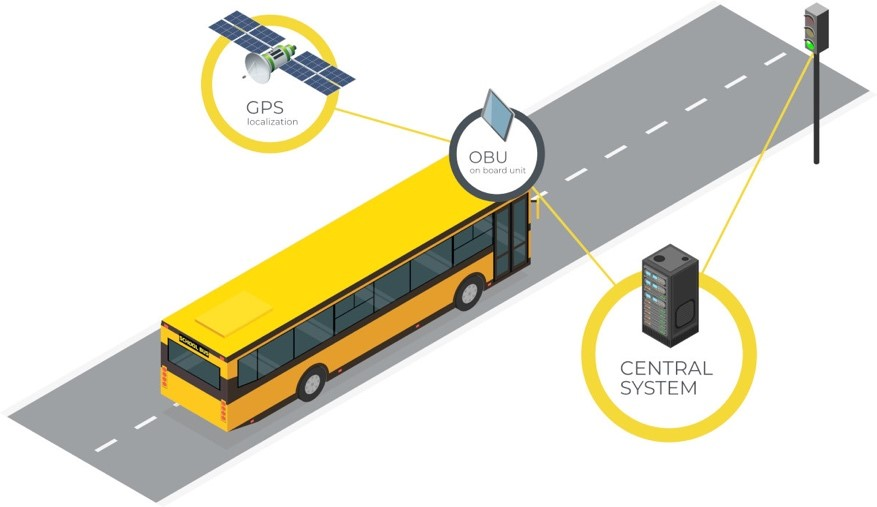
\includegraphics[width=0.7\linewidth]{image/pt_priority_system} \caption{Smart priority for public transport (SWARCO, 2021)}\label{fig:unnamed-chunk-10}
\end{figure}

\hypertarget{relevante-initiativen-in-uxf6sterreich-5}{%
\subsection*{Relevante Initiativen in Österreich}\label{relevante-initiativen-in-uxf6sterreich-5}}
\addcontentsline{toc}{subsection}{Relevante Initiativen in Österreich}

\begin{itemize}
\tightlist
\item
  \href{https://digitales.wien.gv.at/site/open-data/}{digitales.wien.gv.at}
\item
  \href{https://www.wienerlinien.at/eportal3/ep/channelView.do/pageTypeId/66528/channelId/-4400661}{wienerlinien.at}
\item
  \href{https://www.kapsch.net/ktc/Portfolio/IMS/Congestion/Managed-lanes}{kapsch.net-1}
\item
  \href{https://www.kapsch.net/ktc/Portfolio/IMS/Smart-Urban-Mobility/Urban-Mobility-Management}{kapsch.net-2}
\item
  \href{https://www.swarco.com/de/loesungen/oeffentlicher-nahverkehr/vorrang-fuer-den-oeffentlichen-nahverkehr}{swarco.com}
\item
  \href{https://www.mobility.siemens.com/global/de/portfolio/strasse/verkehrsmanagement/auf-der-strasse/smart-detection.html}{mobility.siemens.com}
\end{itemize}

\hypertarget{auswirkungen-in-bezug-auf-die-ziele-fuxfcr-nachhaltige-entwicklung-sdgs-5}{%
\subsection*{Auswirkungen in Bezug auf die Ziele für nachhaltige Entwicklung (SDGs)}\label{auswirkungen-in-bezug-auf-die-ziele-fuxfcr-nachhaltige-entwicklung-sdgs-5}}
\addcontentsline{toc}{subsection}{Auswirkungen in Bezug auf die Ziele für nachhaltige Entwicklung (SDGs)}

\begin{longtable}[]{@{}ccccc@{}}
\toprule
\begin{minipage}[b]{0.17\columnwidth}\centering
Ebene der Auswirkungen\strut
\end{minipage} & \begin{minipage}[b]{0.16\columnwidth}\centering
Indikator\strut
\end{minipage} & \begin{minipage}[b]{0.17\columnwidth}\centering
Richtung der Auswirkungen\strut
\end{minipage} & \begin{minipage}[b]{0.17\columnwidth}\centering
Beschreibung des Ziels \& SDG\strut
\end{minipage} & \begin{minipage}[b]{0.17\columnwidth}\centering
Quelle\strut
\end{minipage}\tabularnewline
\midrule
\endhead
\begin{minipage}[t]{0.17\columnwidth}\centering
Individuell\strut
\end{minipage} & \begin{minipage}[t]{0.16\columnwidth}\centering
Mehr Gleichheit fuer Menschen, die nicht Auto fahren\strut
\end{minipage} & \begin{minipage}[t]{0.17\columnwidth}\centering
\textbf{+}\strut
\end{minipage} & \begin{minipage}[t]{0.17\columnwidth}\centering
Gleichheit (\emph{5,10})\strut
\end{minipage} & \begin{minipage}[t]{0.17\columnwidth}\centering
Litman, 2017; Cervero, 2013\strut
\end{minipage}\tabularnewline
\begin{minipage}[t]{0.17\columnwidth}\centering
Individuell\strut
\end{minipage} & \begin{minipage}[t]{0.16\columnwidth}\centering
Weniger Reisezeit fuer Nutzer:innen oeffentlicher Verkehrsmittel, mehr Reisezeit fuer Pkw-Nutzer\strut
\end{minipage} & \begin{minipage}[t]{0.17\columnwidth}\centering
\textbf{\textasciitilde{}}\strut
\end{minipage} & \begin{minipage}[t]{0.17\columnwidth}\centering
Nachhaltige wirtschaftliche Entwicklung (\emph{8,11})\strut
\end{minipage} & \begin{minipage}[t]{0.17\columnwidth}\centering
Seredynski et al., 2015\strut
\end{minipage}\tabularnewline
\begin{minipage}[t]{0.17\columnwidth}\centering
Systemisch\strut
\end{minipage} & \begin{minipage}[t]{0.16\columnwidth}\centering
Der oeffentliche Verkehr wird im Vergleich zu anderen Verkehrstraegern wettbewerbsfaehiger\strut
\end{minipage} & \begin{minipage}[t]{0.17\columnwidth}\centering
\textbf{+}\strut
\end{minipage} & \begin{minipage}[t]{0.17\columnwidth}\centering
Gleichheit (\emph{5,10})\strut
\end{minipage} & \begin{minipage}[t]{0.17\columnwidth}\centering
Schwendinger, 2019\strut
\end{minipage}\tabularnewline
\begin{minipage}[t]{0.17\columnwidth}\centering
Systemisch\strut
\end{minipage} & \begin{minipage}[t]{0.16\columnwidth}\centering
Weniger Kraftstoffverbrauch\strut
\end{minipage} & \begin{minipage}[t]{0.17\columnwidth}\centering
\textbf{+}\strut
\end{minipage} & \begin{minipage}[t]{0.17\columnwidth}\centering
Oekologische Nachhaltigkeit (\emph{7,12,13,15})\strut
\end{minipage} & \begin{minipage}[t]{0.17\columnwidth}\centering
Gassel et al., 2012; Seredynski et al., 2015\strut
\end{minipage}\tabularnewline
\begin{minipage}[t]{0.17\columnwidth}\centering
Systemisch\strut
\end{minipage} & \begin{minipage}[t]{0.16\columnwidth}\centering
Der Transit ist oft der kostenguenstigste Verkehrstraeger\strut
\end{minipage} & \begin{minipage}[t]{0.17\columnwidth}\centering
\textbf{+}\strut
\end{minipage} & \begin{minipage}[t]{0.17\columnwidth}\centering
Nachhaltige wirtschaftliche Entwicklung (\emph{8,11})\strut
\end{minipage} & \begin{minipage}[t]{0.17\columnwidth}\centering
Litman, 2015\strut
\end{minipage}\tabularnewline
\begin{minipage}[t]{0.17\columnwidth}\centering
Systemisch\strut
\end{minipage} & \begin{minipage}[t]{0.16\columnwidth}\centering
Mehr Infrastruktur fuer den oeffentlichen Verkehr\strut
\end{minipage} & \begin{minipage}[t]{0.17\columnwidth}\centering
\textbf{+}\strut
\end{minipage} & \begin{minipage}[t]{0.17\columnwidth}\centering
Innovation und Infrastruktur (\emph{9})\strut
\end{minipage} & \begin{minipage}[t]{0.17\columnwidth}\centering
Cuthill et al., 2019\strut
\end{minipage}\tabularnewline
\bottomrule
\end{longtable}

\hypertarget{technologie--und-gesellschaftlicher-bereitschaftsgrad-3}{%
\subsection*{Technologie- und gesellschaftlicher Bereitschaftsgrad}\label{technologie--und-gesellschaftlicher-bereitschaftsgrad-3}}
\addcontentsline{toc}{subsection}{Technologie- und gesellschaftlicher Bereitschaftsgrad}

\begin{longtable}[]{@{}cc@{}}
\toprule
Stand der Technologiebereitschaft & Gesellschaftlicher Bereitschaftsgrad\tabularnewline
\midrule
\endhead
4-8 & 5-8\tabularnewline
\bottomrule
\end{longtable}

\hypertarget{offene-fragen-5}{%
\subsection*{Offene Fragen}\label{offene-fragen-5}}
\addcontentsline{toc}{subsection}{Offene Fragen}

\begin{enumerate}
\def\labelenumi{\arabic{enumi}.}
\tightlist
\item
  Wer ist für die Einführung von PTP-Systemen verantwortlich?
\item
  Wie werden Vehicle-to-Vehicle (V2V), Vehicle-to-Infrastructure (V2I) und in Zukunft Vehicle-to-Pedestrian (V2P) PTP-Systeme verändern?
\item
  Wie könnten auch Einsatzfahrzeuge priorisiert werden?
\item
  Wie geht man mit gemischten Flotten um - halb neu, halb alt?
\item
  Was sind die Vorteile im Vergleich zu den Kosten?
\item
  Welche Standards sollten verwendet werden?
\end{enumerate}

\hypertarget{referenzen-5}{%
\subsection*{Referenzen}\label{referenzen-5}}
\addcontentsline{toc}{subsection}{Referenzen}

\begin{itemize}
\tightlist
\item
  Cervero, R. (2013). Bus rapid transit (BRT): An efficient and competitive mode of public transport (No.~2013-01). Working Paper.
\item
  Cuthill, N., Cao, M., Liu, Y., Gao, X., \& Zhang, Y. (2019). The association between urban public transport infrastructure and social equity and spatial accessibility within the urban environment: An investigation of Tramlink in London. Sustainability, 11(5), 1229.
\item
  Figenbaum, E., Fearnley, N., Pfaffenbichler, P., Hjorthol, R., Kolbenstvedt, M., Jellinek, R., \ldots{} \& Iversen, L. M. (2015). Increasing the competitiveness of e-vehicles in Europe. European transport research review, 7(3), 1-14.
\item
  Gassel, C., Matschek, T., \& Krimmling, J. (2012). Cooperative traffic signals for energy efficient driving in tramway systems. Aspekte der Verkehrstelematik--ausgewählte Veröffentlichungen 2012, 1.
\item
  Haitao, H., Yang, K., Liang, H., Menendez, M., \& Guler, S. I. (2019). Providing public transport priority in the perimeter of urban networks: A bimodal strategy. Transportation Research Part C: Emerging Technologies, 107, 171-192.
\item
  Litman, T. (2015). Evaluating public transit benefits and costs. Victoria, BC, Canada: Victoria Transport Policy Institute.
\item
  Litman, T. (2017). Evaluating Transportation Diversity. Victoria Transport Policy Institute.
\item
  Schwendinger, M. (2019). Vorrang für Busse und Straßenbahnen in Städten. \url{https://vcoe.at/files/vcoe/uploads/Projekte/Factsheets} 2019 Neu/VCÖ-Factsheet ÖV-Bevorrangen.pdf
\item
  Seredynski, M., Khadraoui, D., \& Viti, F. (2015, October). Signal phase and timing (SPaT) for cooperative public transport priority measures. In Proc. 22nd ITS World Congress.
\item
  Seredynski, M., Ruiz, P., Szczypiorski, K., \& Khadraoui, D. (2014, May). Improving bus ride comfort using GLOSA-based dynamic speed optimisation. In 2014 IEEE International Parallel \& Distributed Processing Symposium Workshops (pp.~457-463). IEEE.
\item
  Seredynski, M., \& Viti, F. (2017, October). Novel C-ITS support for electric buses with opportunity charging. In 2017 IEEE 20th International Conference on Intelligent Transportation Systems (ITSC) (pp.~1-6). IEEE.
\item
  Stahlmann, R., Möller, M., Brauer, A., German, R., \& Eckhoff, D. (2018). Exploring GLOSA systems in the field: Technical evaluation and results. Computer Communications, 120, 112-124.
\item
  SWARCO. (2021). Vorrang für den ÖPNV: Öffentliche Verkehrsmittel attraktiver machen. Available at: \url{https://www.swarco.com/de/loesungen/oeffentlicher-nahverkehr/vorrang-fuer-den-oeffentlichen-nahverkehr} {[}Accessed: 26 January 2021{]}
\item
  WIENER STADTWERKE GmbH. (2018). Wiener Linien: Autos auf Busspuren halten Ã--ffis auf. Available at: \url{https://www.wienerstadtwerke.at/eportal3/ep/contentView.do?pageTypeId=71954\&channelId=-51313\&programId=72863\&contentId=4202309\&contentTypeId=1001} {[}Accessed: 30 September 2021{]}
\end{itemize}

\hypertarget{transformation_public_space}{%
\section{Transformation des öffentlichen Raums und digitale Lösungen}\label{transformation_public_space}}

\hypertarget{definition-6}{%
\subsection*{Definition}\label{definition-6}}
\addcontentsline{toc}{subsection}{Definition}

Die Digitalisierung des öffentlichen (und städtischen) Raums hat sich entwickelt und zu Konzepten wie Smart City, Wise City, U-City, intelligente Stadt usw. geführt. Die eigentliche Beschleunigung begann jedoch in den 2010er Jahren als Ergebnis von Initiativen der Industrie, die sich auf die Sammlung, Verwaltung, Verarbeitung und Echtzeitanalyse von Big Data durch die weit verbreiteten Sensoren in städtischen Räumen, die als Internet of Things (IoT)-Geräte bekannt sind, konzentrieren. In den letzten Jahren, insbesondere seit dem Ausbruch der COVID-19-Pandemie, hat die Digitalisierung der Städte ein neues Niveau erreicht. So werden beispielsweise in China digitale Systeme zur Massenüberwachung auf der Grundlage der Gesichtserkennung eingesetzt, und in anderen Teilen der Welt wurden Rechtsgrundlagen (wie die Allgemeine Datenschutzverordnung (DSGVO)) entwickelt, um die Erfassung biometrischer Daten im öffentlichen Raum zu ermöglichen (Languillon-Aussel, 2021). Über die Überwachung hinaus wird die Digitalisierung des öffentlichen Raums in vielen verschiedenen Bereichen eingesetzt, z. B. bei Zahlungen und Preisgestaltung, partizipativen Instrumenten oder der Strafverfolgung. So hat Singapur 2020 ein satellitengestütztes städtisches Mautsystem eingeführt, das die Verfolgung jedes Fahrzeugs zu jeder Tageszeit ermöglicht, um eine dynamische Preisgestaltung für die Straßennutzung und den Zonenzugang umzusetzen (Languillon-Aussel, 2021).
Zu den aktuellen Ansätzen für die Digitalisierung des öffentlichen Raums gehören mobile Apps, hochauflösende Kameras, interaktive Stände und Kioske, die Dienstleistungen und Informationen anbieten, aber auch IoT-Geräte wie Sensoren und Beacons, die automatisch Daten sammeln. Diese Geräte haben das Potenzial, die Qualität und den Umfang der Dienstleistungen im öffentlichen Raum zu verbessern, die Bereitstellungs- und Lieferkosten zu senken und die Sicherheit zu erhöhen. Dennoch sind sie nicht ohne Herausforderungen. Potenzielle Probleme ergeben sich aus Datenschutz- und Sicherheitsbedenken, insbesondere wenn der private Sektor eine Schlüsselrolle spielt (Warbis, 2018), aus potenziellen technischen Schwierigkeiten wie unzuverlässigen Internetverbindungen oder instabiler Stromversorgung (Haldrup, 2018) sowie aus geringem Vertrauen unter den Mitgliedern der Gesellschaft und der so genannten digitalen Ausgrenzung bestimmter sozialer Gruppen (Durand \& Zijlstra, 2020).

\hypertarget{wichtige-interessensgruppen-6}{%
\subsection*{Wichtige Interessensgruppen}\label{wichtige-interessensgruppen-6}}
\addcontentsline{toc}{subsection}{Wichtige Interessensgruppen}

\begin{itemize}
\tightlist
\item
  \textbf{Betroffene}: Bürger:innen
\item
  \textbf{Verantwortliche}: Lokale und nationale Regierungen, private Technologieunternehmen, Bürger:innen
\end{itemize}

\hypertarget{aktueller-stand-der-wissenschaft-und-forschung-6}{%
\subsection*{Aktueller Stand der Wissenschaft und Forschung}\label{aktueller-stand-der-wissenschaft-und-forschung-6}}
\addcontentsline{toc}{subsection}{Aktueller Stand der Wissenschaft und Forschung}

Die Forschung zeigt, dass infolge der zunehmenden Digitalisierung des öffentlichen Raums und insbesondere der zunehmenden Digitalisierung des Verkehrs einige Gruppen digital ausgeschlossen werden können. Die Faktoren, die mit der Anfälligkeit in Bezug auf den Zugang zu digital gestützten Dienstleistungen und Verkehrsmitteln verbunden sind, sind:

\begin{itemize}
\tightlist
\item
  \textbf{Alter}: Ältere Menschen und Minderjährige sind aufgrund ihres geringeren Engagements für Technologie besonders benachteiligt. Im Falle der älteren Bevölkerung bedeuten die Verringerung der kognitiven Fähigkeiten und ein Rückgang der psychologischen Mechanismen, dass der Umgang mit neuen Technologien im Allgemeinen schwierig sein kann (Harvey et al., 2019; Pangbourne et al., 2010; Durand \& Zijlstra, 2020). Andererseits haben Kinder häufig keinen Zugang zu digitalen Zahlungsmitteln oder können nicht alle verfügbaren Verkehrsmittel allein nutzen (Durand \& Zijlstra, 2020).
\item
  \textbf{Einkommen und Bildungsniveau}: Menschen mit geringerem Einkommen und Bildungsniveau sind anfälliger für digitale Ausgrenzung, wobei beispielsweise ein niederländischer Bericht zeigt, dass der Übergang vom Offline- zum Online-Kauf eines Jahresabonnements für öffentliche Verkehrsmittel für Menschen mit geringerem Einkommen problematisch ist (Durand \& Zijlstra, 2020).
\item
  \textbf{Ethnische Zugehörigkeit}: Personen, die Minderheiten angehören, sind tendenziell stärker benachteiligt, was jedoch häufig mit anderen Faktoren wie kulturellen Präferenzen oder wirtschaftlicher Benachteiligung zusammenhängt (Durand \& Zijlstra, 2020).
\end{itemize}

\hypertarget{aktueller-stand-der-praktischen-umsetzung-6}{%
\subsection*{Aktueller Stand der praktischen Umsetzung}\label{aktueller-stand-der-praktischen-umsetzung-6}}
\addcontentsline{toc}{subsection}{Aktueller Stand der praktischen Umsetzung}

Zu Beginn stützte sich die Digitalisierung von Städten und öffentlichen Räumen stark auf das verborgene, unterirdische Netz von Kabeln, Sensoren, Steckern und Masten, die im Alltag des Durchschnittsbürgers keine große Rolle spielten. Heutzutage bezieht die Digitalisierung des öffentlichen Raums das Konzept der Smart City in viel größerem Umfang in das tägliche Leben ein. Es gibt viele Möglichkeiten, wie die Digitalisierung im öffentlichen Raum umgesetzt werden kann.

Eine davon ist die verbesserte \textbf{Konnektivität } in Form von Wi-Fi-Hotspots und -Zonen. In New York hat \href{https://www.link.nyc/}{LinkNYC} beispielsweise Konnektivitätskorridore in fünf Bezirken mit mehr als 1700 Verbindungen eingerichtet und damit rund 5 Millionen Nutzer:innen ermöglicht sich kostenlos mit dem schnellsten und stabilsten öffentlichen Glasfasernetz des Landes zu verbinden. Durch diesen Dienst hat LinkNYC den Menschen den Zugang zu Wohltätigkeitsorganisationen, die Nutzung von Behördendiensten und sogar die Bewerbung um einen Arbeitsplatz ermöglicht (Warbis, 2018). Darüber hinaus nutzt \href{https://calvium.com/}{Calvium} die verbesserte Konnektivität, um durch digital-physische Reisen in die Geschichte und das Erbe einen Sinn für den Ort zu schaffen, wie etwa in der \href{https://calvium.com/projects/battersea-power-station-redevelopment/}{Battersea Power Station} in London (Warbis, 2018).

Darüber hinaus bringt die Digitalisierung eine \textbf{Transformation der öffentlichen Dienstleistungen} mit sich, bei der nicht personenbezogene Daten, die im öffentlichen Raum erhoben werden, genutzt werden, um die Nutzer:innen des öffentlichen Raums und ihre Bedürfnisse besser zu verstehen, um die Räume, die Infrastruktur und die Bereitstellung öffentlicher Dienstleistungen in den Städten zu verbessern. Wenn man sich beispielsweise die Art der Geräte ansieht, die mit WiFi-Spots verbunden sind, oder wenn man sich an einem digitalen Platzgestaltungsprogramm beteiligt, kann man sozioökonomische Profile erkennen und die Stadtverwaltungen dabei unterstützen, die richtigen Dienstleistungen für die richtigen Menschen bereitzustellen.

Zwei solcher Beispiele sind (1) der (\emph{1}) \href{https://lbbd.emu-analytics.net/main/(view/950db2c7-1a3b-448d-9b21-444a0ec7b5e0//rightBar:appinfo)?basemapDetail=1\&zoom=5.0\&lng=-0.36613\&lat=54.04187}{Borough Data Explorer}, der Daten für die Indikatoren sammelt, die entweder zu den sogenannten Borough Manifesto-Zielen der Stadt beitragen oder im sozialen Fortschrittsindex der Stadt enthalten sind (Lbbd.emu-analytics.net, 2021). (2) Die australische Stadt Joondalup ist eine Partnerschaft mit \href{https://www.lakesidejoondalup.com.au/store-directory/telstra-shop/}{Telstra} eingegangen, um IoT-Technologien zu testen, mit denen Umweltfaktoren wie Temperatur, Luftfeuchtigkeit, Verschmutzung, Licht- und Lärmpegel in Echtzeit besser überwacht werden können (Barns, 2017).

Als Nächstes ist eine \textbf{öffentlich-private Partnerschaft} von entscheidender Bedeutung für einen starken und zuverlässigen digitalen öffentlichen Bereich, in dem Technologieunternehmen die Politik und Strategie der lokalen Regierung verstehen müssen, um Bereiche zu ermitteln, die durch den digitalen Einsatz unterstützt werden können. Auf der anderen Seite ist es für die Kommunalverwaltung wichtig, die Merkmale der einzusetzenden Technologie zu verstehen. Diese enge Zusammenarbeit ermöglicht es dem öffentlichen Sektor, die Digitalisierung von Orten so zu lenken, dass sie dem öffentlichen Wohl dient und der öffentliche Charakter von Raum und Ort erhalten bleibt, unabhängig davon, wer die eingesetzten Technologien besitzt, beaufsichtigt oder verwaltet (Warbis, 2018). Beispiele für solche Initiativen sind \href{https://wegfinder.at/presse/2021/mit-wegfinder-ist-mobility-as-a-service-in-oesterreich-angekommen(1)/}{Ã--BB360 wegfinder}, \href{https://austriatech.at/en/insight-into-the-work-of-the-urban-mobility-laboratories/}{Living Labs} und \href{https://www.aspern-seestadt.at/en}{Seestadt Wien}.

Innerhalb des Verkehrsnetzes bringt die Digitalisierung Vorteile in Form von verbesserter Individualisierung, Effizienz und Komfort. Beispiele dafür sind Echtzeitinformationen über verfügbare Parkplätze wie \href{https://www.eparkomat.com/}{eParkomat} in der Tschechischen Republik, digitales Ticketing und Fahrplanauskunft wie, \href{https://www.dv-ticketing.com/}{DV Ticketing} oder \href{https://www.thetrainline.com/}{Trainline} in Großbritannien, elektronische Systeme für Car- und Bike-Sharing-Flotten wie \href{https://www.share-now.com/at/en/}{Share-now} oder \href{https://www.nextbike.at/de/niederoesterreich/}{Nextbike} usw. Weitere Informationen über Bike- und Carsharing finden Sie in den Abschnitten über \protect\hyperlink{bike_sharing}{Fahrrad- und E-Bike-Verleih} und \protect\hyperlink{car_sharing}{Car Sharing} in dieser Arbeit.

Schließlich wird behauptet, dass der öffentliche Raum eine politische Funktion hat. In Europa unterstützen und bestimmen sie den Ausdruck des Lebens in der Stadt und spielen eine Rolle bei der partizipativen Planung (Languillon-Aussel, 2021; Parkinson, 2012). So beabsichtigten beispielsweise die österreichischen Eisenbahnen (ÖBB) 2013 den Bau eines\href{https://www.partizipation.at/gueterzentrum_sued.html}{neuen Güterverkehrszentrums} in Wien, das den Güterverkehr von der Straße auf die Schiene verlagern sollte. Das neue Güterverkehrszentrum sollte dasjenige am Nordwestbahnhof ersetzen. Von Anfang an sollte die Öffentlichkeit aktiv in das Projekt einbezogen werden, und die Betroffenen wurden auch stark in die Planung integriert. So gab es vor Projektbeginn eine Informationsveranstaltung der ÖBB, die von großen Protesten (der Bevölkerung) gegen das Projekt begleitet war. Die ÖBB haben wohl gerade deshalb versucht, die Entscheidungsträger:innen so intensiv in den gesamten Planungsprozess einzubinden und haben das Projekt in der Folge erfolgreich abgeschlossen.

Daher kann die Digitalisierung des städtischen Raums die Innovation bei den partizipatorischen Instrumenten beeinflussen, die es den Bürger:innen ermöglichen, ihre Meinung zu äußern und Feedback zu geben, um aktiv zum Infrastrukturplanungsprozess und zur Entscheidungsfindung beizutragen. Dieser Trend führte zur sogenannten digitalen partizipativen Planung (DPP) (Bouzguenda et al., 2020). Einige Beispiele für solche Initiativen sind die App \href{https://mapyour.city/}{Map your city} die Ideenfindungsplattform \href{https://www.involve.org.uk/resources/case-studies/decide-madrid}{Decide Madrid}, \href{https://oscity.nl/}{Open Source City} in den Niederlanden, die britischen Feedback-Plattformen \href{https://www.involve.org.uk/resources/knowledge-base/what/public-participation}{Involve} und \href{http://www.changify.org/}{Changify} oder die Visualisierungsplattform für Argumente namens \href{https://www.nesta.org.uk/feature/six-pioneers-digital-democracy/vtaiwan/}{vTaiwan}.

\hypertarget{relevante-initiativen-in-uxf6sterreich-6}{%
\subsection*{Relevante Initiativen in Österreich}\label{relevante-initiativen-in-uxf6sterreich-6}}
\addcontentsline{toc}{subsection}{Relevante Initiativen in Österreich}

\begin{itemize}
\tightlist
\item
  \href{https://wegfinder.at/presse/2021/mit-wegfinder-ist-mobility-as-a-service-in-oesterreich-angekommen(1)/}{Ã--BB360 wegfinder}
\item
  \href{https://austriatech.at/en/insight-into-the-work-of-the-urban-mobility-laboratories/}{Living Labs}
\item
  \href{https://www.aspern-seestadt.at/en}{Seestadt Wien}
\item
  \href{https://ec.europa.eu/regional_policy/en/projects/Austria/support-for-digital-transformation-in-lower-austria}{House of digitalisation}
\end{itemize}

\hypertarget{auswirkungen-in-bezug-auf-die-ziele-fuxfcr-nachhaltige-entwicklung-sdgs-6}{%
\subsection*{Auswirkungen in Bezug auf die Ziele für nachhaltige Entwicklung (SDGs)}\label{auswirkungen-in-bezug-auf-die-ziele-fuxfcr-nachhaltige-entwicklung-sdgs-6}}
\addcontentsline{toc}{subsection}{Auswirkungen in Bezug auf die Ziele für nachhaltige Entwicklung (SDGs)}

\begin{longtable}[]{@{}ccccc@{}}
\toprule
\begin{minipage}[b]{0.17\columnwidth}\centering
Ebene der Auswirkungen\strut
\end{minipage} & \begin{minipage}[b]{0.16\columnwidth}\centering
Indikator\strut
\end{minipage} & \begin{minipage}[b]{0.17\columnwidth}\centering
Richtung der Auswirkungen\strut
\end{minipage} & \begin{minipage}[b]{0.17\columnwidth}\centering
Beschreibung des Ziels \& SDG\strut
\end{minipage} & \begin{minipage}[b]{0.17\columnwidth}\centering
Quelle\strut
\end{minipage}\tabularnewline
\midrule
\endhead
\begin{minipage}[t]{0.17\columnwidth}\centering
Individuell\strut
\end{minipage} & \begin{minipage}[t]{0.16\columnwidth}\centering
Verschlechterter Zugang zu digital gestuetzten Verkehrsdiensten fuer bestimmte Gruppen\strut
\end{minipage} & \begin{minipage}[t]{0.17\columnwidth}\centering
\textbf{-}\strut
\end{minipage} & \begin{minipage}[t]{0.17\columnwidth}\centering
Gleichheit (\emph{5,10})\strut
\end{minipage} & \begin{minipage}[t]{0.17\columnwidth}\centering
Durand \& Zijlstra, 2020\strut
\end{minipage}\tabularnewline
\begin{minipage}[t]{0.17\columnwidth}\centering
Systemisch\strut
\end{minipage} & \begin{minipage}[t]{0.16\columnwidth}\centering
Geringeres Risiko der verkehrsbedingten sozialen Ausgrenzung\strut
\end{minipage} & \begin{minipage}[t]{0.17\columnwidth}\centering
\textbf{+}\strut
\end{minipage} & \begin{minipage}[t]{0.17\columnwidth}\centering
Gleichheit (\emph{5,10})\strut
\end{minipage} & \begin{minipage}[t]{0.17\columnwidth}\centering
Harvey et al., 2019; Pangbourne et al., 2010\strut
\end{minipage}\tabularnewline
\begin{minipage}[t]{0.17\columnwidth}\centering
Systemisch\strut
\end{minipage} & \begin{minipage}[t]{0.16\columnwidth}\centering
Besser informierte Planung und Entscheidungsfindung auf der Grundlage von Echtzeitdaten aus dem IoT\strut
\end{minipage} & \begin{minipage}[t]{0.17\columnwidth}\centering
\textbf{+}\strut
\end{minipage} & \begin{minipage}[t]{0.17\columnwidth}\centering
Innovation und Infrastruktur (\emph{9})\strut
\end{minipage} & \begin{minipage}[t]{0.17\columnwidth}\centering
Barns, 2017, Bouzguenda et al., 2020\strut
\end{minipage}\tabularnewline
\begin{minipage}[t]{0.17\columnwidth}\centering
Systemisch\strut
\end{minipage} & \begin{minipage}[t]{0.16\columnwidth}\centering
Verstaerkte Zusammenarbeit zwischen oeffentlichem und privatem Sektor\strut
\end{minipage} & \begin{minipage}[t]{0.17\columnwidth}\centering
\textbf{+}\strut
\end{minipage} & \begin{minipage}[t]{0.17\columnwidth}\centering
Partnerschaften und Kooperationen (\emph{17})\strut
\end{minipage} & \begin{minipage}[t]{0.17\columnwidth}\centering
Warbis, 2018;\strut
\end{minipage}\tabularnewline
\bottomrule
\end{longtable}

\hypertarget{technologie--und-gesellschaftlicher-bereitschaftsgrad-4}{%
\subsection*{Technologie- und gesellschaftlicher Bereitschaftsgrad}\label{technologie--und-gesellschaftlicher-bereitschaftsgrad-4}}
\addcontentsline{toc}{subsection}{Technologie- und gesellschaftlicher Bereitschaftsgrad}

\begin{longtable}[]{@{}cc@{}}
\toprule
Stand der Technologiebereitschaft & Gesellschaftlicher Bereitschaftsgrad\tabularnewline
\midrule
\endhead
5-9 & 5-8\tabularnewline
\bottomrule
\end{longtable}

\hypertarget{offene-fragen-6}{%
\subsection*{Offene Fragen}\label{offene-fragen-6}}
\addcontentsline{toc}{subsection}{Offene Fragen}

\begin{enumerate}
\def\labelenumi{\arabic{enumi}.}
\tightlist
\item
  Inwieweit wirkt sich der immer wichtigere Einsatz digitaler Geräte im öffentlichen Raum auf dessen politische Dimensionen aus?
\item
  Verändern die digitalen Technologien die Praktiken der Bürger:innen im öffentlichen Raum und/oder ermöglichen sie das Entstehen neuer Praktiken?
\item
  Indem sie neue Formen der Meinungsäußerung sowie der politischen und demokratischen Teilhabe im Internet ermöglichen, wird der virtuelle Raum tendenziell zu einem neuen Forum. Übernimmt die digitale Technologie die politischen Funktionen des öffentlichen Raums, der dadurch überflüssig geworden ist?
\item
  Welche Auswirkungen haben die kurzen Lebenszyklen der Technologien und der Wechsel der Technologiegenerationen auf die Entwicklung des öffentlichen Raums?
\item
  Verändert die Digitalisierung das Design, die Formen, die Dimensionen und die Räumlichkeit des öffentlichen Raums?
\item
  Auf welche Weise verändert das Aufkommen neuer Werkzeuge und Fähigkeiten die Art und Weise, wie öffentliche Räume geplant und entwickelt werden?
\item
  Welche Rolle spielen digitale Technologien bei der Darstellung, Vorstellung und Wahrnehmung von öffentlichen Räumen?
\item
  Für welche(n) Typ(en) von Empfängern (wie Bürger:innen, Verbraucher:innen, Nutzer:innen und Bewohner:innen) werden digitale Technologien im öffentlichen Raum eingesetzt?
\item
  Welche Auswirkungen haben sie auf die Menschen, die sich im öffentlichen Raum aufhalten?
\item
  Fördern die digitalen Technologien den sozialen Austausch oder vervielfältigen sie im Gegenteil die Segregation der digitalen Blasen?
\item
  Welche Rolle hat die Digitalisierung bei der Anpassung des öffentlichen Raums an die Gesundheitskrise von COVID-19 gespielt? (Languillon-Aussel, 2021)
\end{enumerate}

\hypertarget{weitere-links-4}{%
\subsection*{Weitere links}\label{weitere-links-4}}
\addcontentsline{toc}{subsection}{Weitere links}

\begin{itemize}
\tightlist
\item
  \href{https://agile-city.com/agile-city-research/digital-tools-for-participatory-led-design/}{Agile city}
\item
  \href{https://theconversation.com/surprise-digital-space-isnt-replacing-public-space-and-might-even-help-make-it-better-87173}{An article on city of bits}
\item
  \href{https://archer-soft.com/blog/how-build-real-time-parking-availability-system}{Parking management systems}
\item
  \href{https://jsis.washington.edu/news/internet-of-things-and-privacy-in-public/}{Internet of Things and Privacy in Public}
\end{itemize}

\hypertarget{referenzen-6}{%
\subsection*{Referenzen}\label{referenzen-6}}
\addcontentsline{toc}{subsection}{Referenzen}

\begin{itemize}
\tightlist
\item
  Barns, S. (2017) Surprise! Digital space isn't replacing public space, and might even help make it better. Available at: \url{https://theconversation.com/surprise-digital-space-isnt-replacing-public-space-and-might-even-help-make-it-better-87173} {[}Accessed: 12 April 2021{]}.
\item
  Bouzguenda, I., Alalouch, C., \& Fava, N. (2020). Examining digital participatory planning: maturity assessment in a small Dutch city. Journal of Cleaner Production, 264, 121706.
\item
  Durand, A. \& Zijlstra, T. (2020). The impact of digitalisation on the access to transport services: a literature review. 10.13140/RG.2.2.22686.97600.
\item
  Haldrup, S.,V. (2018). Digitising public service delivery: opportunities and limitations. Available at: \url{https://www.opml.co.uk/blog/digitising-public-service-delivery-opportunities-and-limitations} {[}Accessed: 12 April 2021{]}.
\item
  Harvey, J., Guo, W., \& Edwards, S. (2019). Increasing mobility for older travellers through engagement with technology. Transportation Research Part F: Traffic Psychology and Behaviour, 60, 172-184. \url{doi:10.1016/j.trf.2018.10.019}
\item
  Languillon-Aussel, R. (2021). Digitalisation of public spaces: the great urban change? Available at: \url{https://journals.openedition.org/articulo/4518} . {[}Accessed: 9 April 2021{]}
\item
  Lbbd.emu-analytics.net. (2021). Borough Data Explorer. Available at: \url{https://lbbd.emu-analytics.net/main/(view/950db2c7-1a3b-448d-9b21-444a0ec7b5e0//rightBar:appinfo)?basemapDetail=1\&zoom=4.7\&lng=3.34490\&lat=54.11363} {[}Accessed: 12 April 2021{]}.
\item
  Pangbourne, K. (2018). Mobility and Ageing: A Review of Interactions Between Transport and Technology from the Perspective of Older People In A. Curl \& C. Musselwhite (Eds.), Geographies of Transport and Ageing (pp.~51-71). Cham: Springer International Publishing.
\item
  Parkinson J., 2012, Democracy and Public Space: The Physical Sites of Democratic Performance, Oxford: Oxford University Press, 262 p.
\item
  Warbis, M. (2018). Making the Spaces of Cities Smarter: Why cities (and their citizens) should embrace the digital public realm. \textless Available at: \url{https://medium.com/@warbismichelle/making-the-spaces-of-cities-smarter-why-cities-should-embrace-the-digital-public-realm-c12afc810aaa}\textgreater. {[}Accessed: 12 April 2021{]}
\end{itemize}

\hypertarget{highway}{%
\chapter{Verwaltung der Straßenverkehrsinfrastruktur}\label{highway}}

\hypertarget{uav}{%
\section{Unbemannte Luftfahrzeuge für die Instandhaltung der Infrastruktur}\label{uav}}

\hypertarget{synonyme-6}{%
\subsection*{Synonyme}\label{synonyme-6}}
\addcontentsline{toc}{subsection}{Synonyme}

\emph{Drohnen, ferngesteuerte Fahrzeuge, ferngesteuerte Flugzeuge, Unmanned Aerial Vehicles (UAV)}

\hypertarget{definition-7}{%
\subsection*{Definition}\label{definition-7}}
\addcontentsline{toc}{subsection}{Definition}

Unbemannte Luftfahrzeuge (Unmanned Aerial Vehicles - UAVs), gemeinhin als Drohnen bekannt, sind vielversprechende Technologien, die bei der Inspektion und Datenerfassung für die Instandhaltung und Verwaltung von Infrastrukturen eingesetzt werden können. Dazu gehören zum Beispiel die Erkennung von Verschleiß, die Überwachung des Fortschritts auf einer Autobahnbaustelle oder die Analyse des Verkehrs (Frederiksen et al., 2019). UAVs verfügen in der Regel über eine tragbare Kontrollstation für den menschlichen Bediener, und nach den geltenden Rechtsvorschriften ist ihr Einsatz in städtischen Gebieten auf Flüge innerhalb der Sichtlinie (visual line of sight - VLOS) beschränkt. UAVs verfügen in der Regel über verschiedene Sensoren und Aufzeichnungsgeräte, darunter Video-, Fern- und Nahinfrarot-, Radar- oder Laser-Entfernungsmesser sowie spezielle Kommunikationsgeräte (Shaghlil \& Khalafallah, 2018). Die meisten von ihnen können Echtzeitdaten zwischen dem UAV und der Kontrollstation übertragen. Darüber hinaus verfügen einige von ihnen über zusätzliche Onboard-Datenspeicherfunktionen für eine verbesserte Datenerfassung (Shaghlil \& Khalafallah, 2018). Der Einsatz von Drohnen für infrastrukturbezogene Aufgaben führt nicht nur zu Zeit-, Arbeits- und Kosteneinsparungen, sondern ermöglicht auch eine Verringerung der Risiken, wenn gefährliche Tätigkeiten, die normalerweise von Menschen ausgeführt werden, durch Drohnen ersetzt werden können. Schließlich werden auch die Umweltauswirkungen verringert, wenn Drohnen, die erheblich weniger CO\textsubscript{2} produzieren, anstelle der derzeit eingesetzten Hubschrauber eingesetzt werden. Dennoch kann der Einsatz von Drohnen als Instrument zur Inspektion von Infrastrukturen auch gewisse Herausforderungen in Bezug auf die derzeitige Technologie, den rechtlichen Rahmen, den Schutz der Privatsphäre und die gesellschaftliche Akzeptanz mit sich bringen.

\hypertarget{wichtige-interessensgruppen-7}{%
\subsection*{Wichtige Interessensgruppen}\label{wichtige-interessensgruppen-7}}
\addcontentsline{toc}{subsection}{Wichtige Interessensgruppen}

\begin{itemize}
\tightlist
\item
  \textbf{Betroffene}: Direkte Nutzer:innen der Straßen und Begünstigte, die von der Erbringung von Verkehrsdienstleistungen betroffen sind
\item
  \textbf{Verantwortliche}: Staatliche Stellen, die für die Planung, Durchführung und Finanzierung von Instandhaltungsmaßnahmen zuständig sind, Bürger:innen, Auftragnehmer:innen und Unterauftragnehmer:innen, Privatunternehmen und Hersteller
\end{itemize}

\hypertarget{aktueller-stand-der-wissenschaft-und-forschung-7}{%
\subsection*{Aktueller Stand der Wissenschaft und Forschung}\label{aktueller-stand-der-wissenschaft-und-forschung-7}}
\addcontentsline{toc}{subsection}{Aktueller Stand der Wissenschaft und Forschung}

Aktuelle Forschungsanstrengungen und auf Feldversuchen basierende Studien sprechen für den Einsatz von UAVs zur Brückeninspektion und -überwachung. In einer früheren Studie wurde ein Konzeptnachweis für den Einsatz von UAVs für Brücken- und Hochmastleuchten vorgelegt. Es wurden mehrere Experimente unter kontrollierten Bedingungen durchgeführt, um das Verhalten von UAVs in Abhängigkeit von den Windverhältnissen zu testen. Außerdem wurde die Bildqualität in verschiedenen Flugszenarien, bei schlechten Lichtverhältnissen, in verschiedenen Höhen und mit unterschiedlicher Nutzlast untersucht (Otero et al., 2015). Insgesamt sprechen die Ergebnisse für den Einsatz von Drohnen bei Infrastrukturinspektionen, nicht nur im Hinblick auf die Einsparung menschlicher Arbeitskraft, sondern auch auf die Erkennung von Schäden. Die Vorteile des Drohneneinsatzes wurden auch im Hinblick auf eine geringere Verkehrskontrolle und einen geringeren Einsatz von Inspektionsfahrzeugen unter Brücken nachgewiesen (Zink und Lovelace, 2015). Andererseits wurde festgestellt, dass der Mangel an spezifischen Fähigkeiten der Drohnenbediener den effizienten Einsatz von Drohnen für große Brücken behindert (Wu et al., 2018). Darüber hinaus bremsen auch einige technologische Barrieren die Popularität von Drohnen bei der Infrastrukturinspektion, wobei die durchschnittliche Flugzeit der Drohne angesichts ihrer Akkulaufzeit etwa 30 Minuten beträgt. Daher zielt die aktuelle Forschung darauf ab, die Energieeffizienz durch den Einsatz von Pfadplanung und Algorithmen zur Minimierung des Energieverbrauchs bei gleichzeitiger Maximierung der Abdeckung für die Verkehrsüberwachung zu erhöhen (Outay et al., 2020).

\hypertarget{aktueller-stand-der-praktischen-umsetzung-7}{%
\subsection*{Aktueller Stand der praktischen Umsetzung}\label{aktueller-stand-der-praktischen-umsetzung-7}}
\addcontentsline{toc}{subsection}{Aktueller Stand der praktischen Umsetzung}

Die derzeitige Nutzung von Drohnen wird von nationalen und internationalen Regierungen weltweit stark reguliert, wobei die größte Einschränkung darin besteht, dass die Drohnen in der VLOS-Position des Fluglotsen bleiben müssen. Darüber hinaus legen die Regulierungsbehörden verschiedene Spezifikationen in Bezug auf physische Aspekte der Drohnen wie Gewicht oder Sensoren, Schulungsanforderungen für Betreiber und Drohnen, Vorschriften für die Datenerfassung und den Betrieb selbst wie Flugdauer, Flughöhe usw. vor. (FAA, 2016; Outay at al., 2020). Alle diese Faktoren schränken die schnelle und breite Anwendung von Drohnen in verschiedenen Bereichen erheblich ein. Daher versuchen die Behörden, Vorschriften zu erlassen, um die Bedenken der Bürger:innen in Bezug auf Sicherheit, Privatsphäre und Lärm zu zerstreuen. Gegenwärtig werden Drohnen in der Öl- und Gasindustrie eingesetzt, um lokale Erhebungen in Offshore-Anlagen durchzuführen (Unternehmen, 2016). Im Verkehrssektor hat das dänische Unternehmen Dronops nach einer Sicherheitsüberprüfung von der dänischen Straßenverkehrsbehörde die Genehmigung erhalten, entlang einer Autobahn zu fliegen, um den Verkehr zu überwachen, wobei die Drohne Daten von mehreren Sensoren sowie Videoaufnahmen liefert. Derzeit kann die Drohne nur bei guten Wetterbedingungen fliegen und ist per Kabel mit ihrer Stromquelle am Boden verbunden, um eine kontinuierliche Überwachung in 120 m Höhe den ganzen Tag lang zu ermöglichen. Wichtig ist, dass die ausgegebenen Daten von der dänischen Straßenverkehrsbehörde und der Gemeindeverwaltung verwendet werden (Frederiksen et al., 2019).

\hypertarget{relevante-initiativen-in-uxf6sterreich-7}{%
\subsection*{Relevante Initiativen in Österreich}\label{relevante-initiativen-in-uxf6sterreich-7}}
\addcontentsline{toc}{subsection}{Relevante Initiativen in Österreich}

\begin{itemize}
\tightlist
\item
  \href{https://smartcity.wien.gv.at/site/en/smart-inspection/}{smartcity.wien}
\end{itemize}

\hypertarget{auswirkungen-in-bezug-auf-die-ziele-fuxfcr-nachhaltige-entwicklung-sdgs-7}{%
\subsection*{Auswirkungen in Bezug auf die Ziele für nachhaltige Entwicklung (SDGs)}\label{auswirkungen-in-bezug-auf-die-ziele-fuxfcr-nachhaltige-entwicklung-sdgs-7}}
\addcontentsline{toc}{subsection}{Auswirkungen in Bezug auf die Ziele für nachhaltige Entwicklung (SDGs)}

\begin{longtable}[]{@{}ccccc@{}}
\toprule
\begin{minipage}[b]{0.17\columnwidth}\centering
Ebene der Auswirkungen\strut
\end{minipage} & \begin{minipage}[b]{0.16\columnwidth}\centering
Indikator\strut
\end{minipage} & \begin{minipage}[b]{0.17\columnwidth}\centering
Richtung der Auswirkungen\strut
\end{minipage} & \begin{minipage}[b]{0.17\columnwidth}\centering
Beschreibung des Ziels \& SDG\strut
\end{minipage} & \begin{minipage}[b]{0.17\columnwidth}\centering
Quelle\strut
\end{minipage}\tabularnewline
\midrule
\endhead
\begin{minipage}[t]{0.17\columnwidth}\centering
Individuell\strut
\end{minipage} & \begin{minipage}[t]{0.16\columnwidth}\centering
Verringerung des Risikos fuer Arbeitnehmer\strut
\end{minipage} & \begin{minipage}[t]{0.17\columnwidth}\centering
\textbf{+}\strut
\end{minipage} & \begin{minipage}[t]{0.17\columnwidth}\centering
Gesundheit und Wohlbefinden (\emph{3})\strut
\end{minipage} & \begin{minipage}[t]{0.17\columnwidth}\centering
Outay et al., 2020\strut
\end{minipage}\tabularnewline
\begin{minipage}[t]{0.17\columnwidth}\centering
Systemisch\strut
\end{minipage} & \begin{minipage}[t]{0.16\columnwidth}\centering
Erhoehung der Verkehrssicherheit\strut
\end{minipage} & \begin{minipage}[t]{0.17\columnwidth}\centering
\textbf{+}\strut
\end{minipage} & \begin{minipage}[t]{0.17\columnwidth}\centering
Gesundheit und Wohlbefinden (\emph{3})\strut
\end{minipage} & \begin{minipage}[t]{0.17\columnwidth}\centering
Outay et al., 2020\strut
\end{minipage}\tabularnewline
\begin{minipage}[t]{0.17\columnwidth}\centering
Systemisch\strut
\end{minipage} & \begin{minipage}[t]{0.16\columnwidth}\centering
Verringerte Emissionsrate\strut
\end{minipage} & \begin{minipage}[t]{0.17\columnwidth}\centering
\textbf{+}\strut
\end{minipage} & \begin{minipage}[t]{0.17\columnwidth}\centering
Oekologische Nachhaltigkeit (\emph{7,12,13,15})\strut
\end{minipage} & \begin{minipage}[t]{0.17\columnwidth}\centering
Outay et al., 2020\strut
\end{minipage}\tabularnewline
\begin{minipage}[t]{0.17\columnwidth}\centering
Systemisch\strut
\end{minipage} & \begin{minipage}[t]{0.16\columnwidth}\centering
Schaffung von Arbeitsplaetzen\strut
\end{minipage} & \begin{minipage}[t]{0.17\columnwidth}\centering
\textbf{+}\strut
\end{minipage} & \begin{minipage}[t]{0.17\columnwidth}\centering
Nachhaltige wirtschaftliche Entwicklung (\emph{8,11})\strut
\end{minipage} & \begin{minipage}[t]{0.17\columnwidth}\centering
Jenkins \& Vasigh, 2013\strut
\end{minipage}\tabularnewline
\begin{minipage}[t]{0.17\columnwidth}\centering
Systemisch\strut
\end{minipage} & \begin{minipage}[t]{0.16\columnwidth}\centering
Schnellere Innovation der Strasseninfrastruktur\strut
\end{minipage} & \begin{minipage}[t]{0.17\columnwidth}\centering
\textbf{+}\strut
\end{minipage} & \begin{minipage}[t]{0.17\columnwidth}\centering
Innovation und Infrastruktur (\emph{9})\strut
\end{minipage} & \begin{minipage}[t]{0.17\columnwidth}\centering
Fan \& Saadeghvaziri, 2019\strut
\end{minipage}\tabularnewline
\bottomrule
\end{longtable}

\hypertarget{technologie--und-gesellschaftlicher-bereitschaftsgrad-5}{%
\subsection*{Technologie- und gesellschaftlicher Bereitschaftsgrad}\label{technologie--und-gesellschaftlicher-bereitschaftsgrad-5}}
\addcontentsline{toc}{subsection}{Technologie- und gesellschaftlicher Bereitschaftsgrad}

\begin{longtable}[]{@{}cc@{}}
\toprule
Stand der Technologiebereitschaft & Gesellschaftlicher Bereitschaftsgrad\tabularnewline
\midrule
\endhead
3-4 & 5-7\tabularnewline
\bottomrule
\end{longtable}

\hypertarget{offene-fragen-7}{%
\subsection*{Offene Fragen}\label{offene-fragen-7}}
\addcontentsline{toc}{subsection}{Offene Fragen}

\begin{enumerate}
\def\labelenumi{\arabic{enumi}.}
\tightlist
\item
  Welche Faktoren beeinflussen die gesellschaftliche Akzeptanz von Drohnen?
\item
  Welche Maßnahmen müssen von den politischen Entscheidungsträger:innenn ergriffen werden, um Cyberangriffe auf ein Minimum zu reduzieren?
\item
  Welche Aspekte müssen von den Regierungen vor der Integration weiterer Sensoren zur Aufzeichnung anderer relevanter Daten sowie der Integration von Videodaten mit anderen Geodaten berücksichtigt werden?
\end{enumerate}

\hypertarget{weitere-links-5}{%
\subsection*{Weitere links}\label{weitere-links-5}}
\addcontentsline{toc}{subsection}{Weitere links}

\begin{itemize}
\tightlist
\item
  \href{https://www.rolandberger.com/en/Insights/Publications/Drones-The-future-of-asset-inspection.html}{rolandberger}
\end{itemize}

\hypertarget{referenzen-7}{%
\subsection*{Referenzen}\label{referenzen-7}}
\addcontentsline{toc}{subsection}{Referenzen}

\begin{itemize}
\tightlist
\item
  FAA News, 2016, Summary of Small Unmanned Aircraft Rule (Part 107), Federal Aviation Authority, Washington DC, 20591, Accessed on May 2020, \url{https://www.faa.gov/uas/media/Part_107_Summary.pdf}.
\item
  Fan, J., \& Saadeghvaziri, M. A. (2019). Applications of Drones in Infrastructures: Challenges and Opportunities. International Journal of Mechanical and Mechatronics Engineering, 13(10), 649-655.
\item
  Frederiksen, M. H., Mouridsen, O. A. V., \& Knudsen, M. P. (2019). Drones for inspection of infrastructure: Barriers, opportunities and successful uses.
\item
  Jenkins, D., \& Vasigh, B. (2013). The economic impact of unmanned aircraft systems integration in the United States. Association for Unmanned Vehicle Systems International (AUVSI).
\item
  Otero, L.D., Gagliardo, N., Dalli, D., Huang, W.-H., Cosentino, P. (2015). Proof of concept for using unmanned aerial vehicles for high mast pole and bridge inspections (No.~BDV28-977-02). Florida. Dept. of Transportation. Research Center.
\item
  Outay, F., Mengash, H. A., \& Adnan, M. (2020). Applications of unmanned aerial vehicle (UAV) in road safety, traffic and highway infrastructure management: Recent advances and challenges. Transportation research. Part A, Policy and practice, 141, 116-129. \url{https://doi.org/10.1016/j.tra.2020.09.018}
\item
  Shaghlil, N., \& Khalafallah, A. (2018). Automating highway infrastructure maintenance using unmanned aerial vehicles. In Construction Research Congress (2-4).
\item
  Undertaking, S. J. (2016). European drones outlook study. Unlocking the Value for Europe.
\item
  Wu, W., Qurishee, M. A., Owino, J., Fomunung, I., Onyango, M., Atolagbe, B. (2018). Coupling deep learning and UAV for infrastructure condition assessment automation. In: 2018 IEEE International Smart Cities Conference (ISC2). IEEE, pp.~1-7.
\item
  Zink, J. and Lovelace, B., 2015. Unmanned aerial vehicle bridge inspection demonstration project. Research Project. Final Report, 40. Accessed in Nov 2020
\end{itemize}

\hypertarget{charging_station}{%
\section{Elektrische Ladestationen}\label{charging_station}}

\hypertarget{synonyme-7}{%
\subsection*{Synonyme}\label{synonyme-7}}
\addcontentsline{toc}{subsection}{Synonyme}

\emph{Ladestation für Elektrofahrzeuge (EV -- electric vehicle), EV-Ladestation, elektrische Ladestation, Ladepunkt, elektronische Ladestation (ECS - electronic charging station), Versorgungseinrichtung für Elektrofahrzeuge (EVSE - electric vehicle supply equipment)}

\hypertarget{definition-8}{%
\subsection*{Definition}\label{definition-8}}
\addcontentsline{toc}{subsection}{Definition}

Heutzutage nimmt die Nutzung von Elektrofahrzeugen kontinuierlich zu. Daher ist es nicht verwunderlich, dass sowohl Regierungen als auch private Unternehmen ein starkes Interesse am Ausbau der Ladeinfrastruktur für Elektrofahrzeuge haben, um eine ununterbrochene Fahrt zu gewährleisten und die Akzeptanz der Verbraucher:innen zu fördern. Es gibt drei Haupttypen von Ladestationen, abhängig von der Ausgangsleistung (gemessen in Kilowatt (kW)) und der daraus resultierenden Ladegeschwindigkeit. Diese sind:

\begin{itemize}
\tightlist
\item
  \textbf{High-Power Charging (Rapid)}
\end{itemize}

Sie sind die schnellste Art, ein Elektroauto aufzuladen, und werden daher am häufigsten in der Nähe von Hauptverkehrsstraßen und an Autobahnraststätten aufgestellt. Sie verfügen über ein fest verlegtes Kabel und eine hohe Leistung in Form von Gleichstrom (DC) oder Wechselstrom (AC). Fahrzeuge können in etwa 20 Minuten bis zu 80\% aufgeladen werden, aber im Durchschnitt dauert es etwa eine Stunde für ein neues Elektrofahrzeug. DC-Schnellladegeräte verwenden entweder \href{https://chademo.com/}{CHAdeMO} - oder CCS-Ladestandards. Dies sind die beiden derzeit am häufigsten verwendeten Typen. Sie bieten eine Leistung von 50 kW. Ein neuerer Typ sind Ultra \emph{Rapid DC-Ladegeräte}, die eine Leistung von mindestens 100 kW haben. Außerdem bieten \emph{AC-Schnellladegeräte} eine Leistung von 43 kW und verwenden den \href{https://www.mobilityhouse.com/int_en/knowledge-center/charging-cable-and-plug-types\#:~:text=Type\%202\%20plug,-The\%20triple\%2Dphase\&text=In\%20private\%20spaces\%2C\%20charging\%20power,with\%20a\%20type\%202\%20socket.}{Typ 2} Ladestandard. Ein spezielles Netz von Ladegeräten schließlich sind die \emph{Supercharger von Tesla}, die speziell für Tesla-Fahrzeuge hergestellt werden. Dennoch verwenden viele Tesla-Fahrer:innen Adapter, die es ihnen ermöglichen, weit verbreitete generische Ladegeräte zu nutzen (Lilly, 2020).

\begin{itemize}
\tightlist
\item
  \textbf{Schnellladung (Fast)}
\end{itemize}

Schnellladestationen bieten in der Regel eine AC-Ladung mit einer Ausgangsleistung von 7 kW oder 22 kW. Es gibt jedoch auch Stationen, die 25-kW-Gleichstromladegeräte mit CHAdeMO- oder CCS-Ladestandards verwenden. Die Ladezeiten liegen zwischen 1 und 6 Stunden, abhängig von der im Fahrzeug installierten Batterie. Schnellladestationen befinden sich in der Regel auf Parkplätzen, in Supermärkten oder Freizeitzentren, wo die Autos wahrscheinlich eine Stunde oder länger abgestellt werden. Schnellladestationen können sowohl angebunden als auch nicht angebunden sein (Lilly, 2020).

\begin{itemize}
\tightlist
\item
  \textbf{Langsam}
\end{itemize}

Die Leistung von Langsamladegeräten variiert zwischen 2,3 kW und 6 kW und dauert zwischen 6 und 12 Stunden. Die meisten Langsamladegeräte sind kabellos, d.~h. Fahrer:innen müssen ein eigenes Kabel mitbringen, um das Elektrofahrzeug mit der Ladestation zu verbinden. Sie werden in der Regel zum Aufladen zu Hause über Nacht, aber auch am Arbeitsplatz und an öffentlichen Ladestationen verwendet. Aufgrund der längeren Ladezeiten im Vergleich zu Schnellladegeräten sind langsame öffentliche Ladepunkte weniger verbreitet und können ältere Geräte sein.

Die hohen Investitionskosten (einschließlich Grunderwerb, Installation, Betrieb und Wartung) und die geringe Rentabilität (die stark von ihrer Nutzung abhängt) gelten jedoch als Haupthindernisse für eine schnellere Entwicklung von Ladestationen (Lilly, 2020).

\hypertarget{wichtige-interessensgruppen-8}{%
\subsection*{Wichtige Interessensgruppen}\label{wichtige-interessensgruppen-8}}
\addcontentsline{toc}{subsection}{Wichtige Interessensgruppen}

\begin{itemize}
\tightlist
\item
  \textbf{Betroffene}: EV-Fahrer:innen
\item
  \textbf{Verantwortliche}: Nationale Unternehmen und Regierungen, internationale Öl- und Gasunternehmen, Automobilunternehmen, Start-ups im Bereich der grünen Energie, Verkehrsbehörden
\end{itemize}

\hypertarget{aktueller-stand-der-wissenschaft-und-forschung-8}{%
\subsection*{Aktueller Stand der Wissenschaft und Forschung}\label{aktueller-stand-der-wissenschaft-und-forschung-8}}
\addcontentsline{toc}{subsection}{Aktueller Stand der Wissenschaft und Forschung}

Ladestationen für Elektrofahrzeuge sind inzwischen eine gut etablierte Technologie für sich. Daher konzentriert sich die aktuelle Forschung auf die Erforschung ihres Potenzials in Kombination mit anderen neuen Technologien. Lokhandwala \& Cai (2020) beispielsweise verwenden Taxis in New York City als Fallstudie, um mögliche Wechselwirkungen zwischen Ladeinfrastruktur für Elektrofahrzeuge, Ride Sharing (RS) und automatisierten Fahrzeugen (AV) zu untersuchen. Zu diesem Zweck vergleichen sie die optimalen Ausbaupläne für die Ladeinfrastruktur für drei Fälle: ein Nicht-AV-RS-Szenario (Gegenwart), ein AV-RS-Szenario (Zukunft) und einen Mischfall. Die Simulation der Studie zeigt, dass im AV-RS-Fall die Nutzung der Ladestationen stärker über den Tag verteilt ist als im Nicht-AV-RS-Fall, wo die Nachfrage und die Warteschlangen morgens am größten sind. In Bezug auf das Dienstleistungsniveau zeigt sich, dass im Nicht-AV-RS-Szenario das Dienstleistungsniveau infolge der Einführung von E-Fahrzeugen unverändert blieb, während es im AV-RS-Fall um 2\% sank. Schließlich zeigt die Studie, dass EV-Taxis in beiden Szenarien eine Reduzierung der CO\textsubscript{2}-Emissionen erwarten lassen.

Darüber hinaus konzentriert sich ein großer Teil der Forschung auf die Optimierung der Standorte von Ladestationen für verschiedene Fahrzeugtypen wie Taxis (Zhang et al., 2019), Busse (Uslu \& Kaya, 2021; Wu et al., 2021; He et al., 2019) und private E-Fahrzeuge (Pan et al., 2020) unter Berücksichtigung verschiedener Faktoren, wie z.B. der sozialen Akzeptanz, der Akzeptanz von E-Fahrzeugen, der Nachfrageschwankungen, der Länge der Fahrten (Anjos et al., 2020) und der Art der Straßeninfrastruktur, einschließlich Autobahnen (Napoli et al., 2020) und städtischer Netze (Ji et al., 2020).

Schließlich befasst sich ein wichtiger Teil der Forschung mit der Rolle der Ladestationsinfrastruktur bei der Einführung und Nutzung von Elektrofahrzeugen, die als Lösung zur Verringerung von Treibhausgasemissionen und Luftverschmutzung angesehen werden (Philipsen et al., 2019; Bonges et al., 2016). Die Studie von Melliger et al.~(2018) untersuchte beispielsweise, wie der Ausbau des Ladestationsnetzes dem Phänomen der sogenannten \emph{``Reichweitenangst''} bei E-Fahrzeugkäufer:innen entgegenwirken kann, das mit der Kapazität der E-Fahrzeugbatterie und der Verfügbarkeit von Ladestationen entlang der Routen zusammenhängt (Melliger et al., 2018).

\hypertarget{aktueller-stand-der-praktischen-umsetzung-8}{%
\subsection*{Aktueller Stand der praktischen Umsetzung}\label{aktueller-stand-der-praktischen-umsetzung-8}}
\addcontentsline{toc}{subsection}{Aktueller Stand der praktischen Umsetzung}

Laut dem Global EV outlook 2020 (IEA, 2020) erreichte die Anzahl der weltweiten Ladestationen im Jahr 2019 7,3 Millionen Ladegeräte. Davon sind 6,5 Millionen langsame und normale Ladestationen, die in Haushalten, Wohn- und Bürogebäuden installiert sind, während der Rest öffentlich zugängliche Ladestationen sind (Thananusak et al., 2021).

Es hat sich gezeigt, dass ein dichteres Netz von Ladestationen ein wichtiger Faktor ist, um die Reichweitenangst der Nutzer:innen von Elektrofahrzeugen zu verringern (Philipsen et al., 2019). Daher ist es nicht verwunderlich, dass die Politik vieler Länder in Europa und darüber hinaus Ziele für den Bau von Ladestationen für Elektrofahrzeuge gesetzt hat, um deren Verbreitung zu fördern. So hat Frankreich beispielsweise das sogenannte \href{https://www.iea.org/policies/8737-law-on-energy-transition-for-green-growth-ltecv}{Gesetz zur Energiewende für grünes Wachstum (LTECV)} eingeführt, das den Bau von 7 Millionen Ladestationen bis 2030 vorsieht (Thananusak et al., 2021). In der Schweiz empfahl das Bundesamt für Straßen (ASTRA) die Installation von Schnellladestationen an allen wichtigen Autobahnraststätten (Melliger et al., 2018). In Bezug auf die EU-weite Gesetzgebung verpflichtet die \emph{\href{https://eur-lex.europa.eu/legal-content/EN/TXT/HTML/?uri=CELEX:32014L0094\&from=en}{Richtlinie 2014/94/EU} über den Aufbau einer Infrastruktur für das Aufladen und Betanken mit alternativen Kraftstoffen} (bekannt als Alternative Fuels Infrastructure Directive (AFI)) die EU-Mitgliedsstaaten dazu, eine angemessene Anzahl von öffentlich zugänglichen Ladepunkten bereitzustellen.
Im österreichischen Kontext hat die Studie von Baresch \& Moser (2019) gezeigt, dass 88\% der E-Fahrzeugnutzer ihr Auto zu Hause aufladen und nur 1,5\% - 1,7\% öffentliche Stationen nutzen. Dies hat einen erheblichen Einfluss auf die Rentabilität der öffentlichen Ladestationen. Um dieses Problem zu lindern, können Regierungen nachfragefördernde oder technologiefördernde Maßnahmen ergreifen. Die nachfragefördernden Lösungen basieren auf der Ausweitung der Märkte für Innovationen, um die Nachfrage zu steigern und die Gewinne aus dem Geschäft mit Ladestationen zu erhöhen. Dazu gehören z. B. die Sensibilisierung der Verbraucher:innen, Rabatte und Steuergutschriften. Auf der anderen Seite zielen die Technologie-Push-Lösungen darauf ab, die Kosten für innovative Lösungen durch Finanzierung und Subventionen für F\&E im privaten Sektor zu senken (Thananusak et al., 2021).
Interessanterweise fand zwischen 2007 und 2013 das erste transnationale Elektromobilitätsprojekt zwischen Wien und Bratislava statt. Es zielte darauf ab, die Funktionsfähigkeit einer grenzüberschreitenden Initiative zu demonstrieren. Zu diesem Zweck wurde eine Reihe von Ladestationen an öffentlichen und halböffentlichen Orten errichtet, damit Nutzer:innen von Elektrofahrzeugen ihre Fahrzeuge auf beiden Seiten der Grenze aufladen können. Das Projekt zeigte die Benutzerfreundlichkeit von Elektrofahrzeugen im täglichen Verkehr und die grenzüberschreitende Verfügbarkeit von Dienstleistungen, unabhängig vom Wohnsitzland des E-Mobilitätskunden (Verbund, 2011).

\hypertarget{relevante-initiativen-in-uxf6sterreich-8}{%
\subsection*{Relevante Initiativen in Österreich}\label{relevante-initiativen-in-uxf6sterreich-8}}
\addcontentsline{toc}{subsection}{Relevante Initiativen in Österreich}

\begin{itemize}
\tightlist
\item
  \href{http://www.ieahev.org/by-country/austria-charging-infrastructure/}{ieahev.org}
\item
  \href{https://ev-charging.com/at/en/elektrotankstellen}{ev-charging.com}
\item
  \href{https://smatrics.com/en/charging-network}{smatrics.com}
\item
  \href{https://chargemap.com/cities/wien-AT}{chargemap.com}
\end{itemize}

\hypertarget{auswirkungen-in-bezug-auf-die-ziele-fuxfcr-nachhaltige-entwicklung-sdgs-8}{%
\subsection*{Auswirkungen in Bezug auf die Ziele für nachhaltige Entwicklung (SDGs)}\label{auswirkungen-in-bezug-auf-die-ziele-fuxfcr-nachhaltige-entwicklung-sdgs-8}}
\addcontentsline{toc}{subsection}{Auswirkungen in Bezug auf die Ziele für nachhaltige Entwicklung (SDGs)}

\begin{longtable}[]{@{}ccccc@{}}
\toprule
\begin{minipage}[b]{0.17\columnwidth}\centering
Ebene der Auswirkungen\strut
\end{minipage} & \begin{minipage}[b]{0.16\columnwidth}\centering
Indikator\strut
\end{minipage} & \begin{minipage}[b]{0.17\columnwidth}\centering
Richtung der Auswirkungen\strut
\end{minipage} & \begin{minipage}[b]{0.17\columnwidth}\centering
Beschreibung des Ziels \& SDG\strut
\end{minipage} & \begin{minipage}[b]{0.17\columnwidth}\centering
Quelle\strut
\end{minipage}\tabularnewline
\midrule
\endhead
\begin{minipage}[t]{0.17\columnwidth}\centering
Systemisch\strut
\end{minipage} & \begin{minipage}[t]{0.16\columnwidth}\centering
Beitrag zur Emissionsminderung (durch EVs)\strut
\end{minipage} & \begin{minipage}[t]{0.17\columnwidth}\centering
\textbf{+}\strut
\end{minipage} & \begin{minipage}[t]{0.17\columnwidth}\centering
Oekologische Nachhaltigkeit (\emph{7,12,13,15})\strut
\end{minipage} & \begin{minipage}[t]{0.17\columnwidth}\centering
Thananusak et al., 2021\strut
\end{minipage}\tabularnewline
\begin{minipage}[t]{0.17\columnwidth}\centering
Systemisch\strut
\end{minipage} & \begin{minipage}[t]{0.16\columnwidth}\centering
Mehr oeffentliche Mittel fuer Ladestationen, aber hohe Einstiegshuerden fuer Investoren\strut
\end{minipage} & \begin{minipage}[t]{0.17\columnwidth}\centering
\textbf{\textasciitilde{}}\strut
\end{minipage} & \begin{minipage}[t]{0.17\columnwidth}\centering
Innovation und Infrastruktur (\emph{9})\strut
\end{minipage} & \begin{minipage}[t]{0.17\columnwidth}\centering
Thananusak et al., 2021\strut
\end{minipage}\tabularnewline
\begin{minipage}[t]{0.17\columnwidth}\centering
Systemisch\strut
\end{minipage} & \begin{minipage}[t]{0.16\columnwidth}\centering
Foerderung der Zusammenarbeit zwischen verschiedenen Interessengruppen (z. B. Industrie und Regierungen) und Laendern\strut
\end{minipage} & \begin{minipage}[t]{0.17\columnwidth}\centering
\textbf{+}\strut
\end{minipage} & \begin{minipage}[t]{0.17\columnwidth}\centering
Partnerschaften und Kooperationen (\emph{17})\strut
\end{minipage} & \begin{minipage}[t]{0.17\columnwidth}\centering
Thananusak et al., 2021\strut
\end{minipage}\tabularnewline
\bottomrule
\end{longtable}

\hypertarget{technologie--und-gesellschaftlicher-bereitschaftsgrad-6}{%
\subsection*{Technologie- und gesellschaftlicher Bereitschaftsgrad}\label{technologie--und-gesellschaftlicher-bereitschaftsgrad-6}}
\addcontentsline{toc}{subsection}{Technologie- und gesellschaftlicher Bereitschaftsgrad}

\begin{longtable}[]{@{}cc@{}}
\toprule
Stand der Technologiebereitschaft & Gesellschaftlicher Bereitschaftsgrad\tabularnewline
\midrule
\endhead
8-9 & 6-8\tabularnewline
\bottomrule
\end{longtable}

\hypertarget{offene-fragen-8}{%
\subsection*{Offene Fragen}\label{offene-fragen-8}}
\addcontentsline{toc}{subsection}{Offene Fragen}

\begin{enumerate}
\def\labelenumi{\arabic{enumi}.}
\tightlist
\item
  Was sind nachfragefördernde und technologiefördernde Maßnahmen zur Steigerung der Investitionen in Ladestationen? Wie hoch ist ihre relative Wirksamkeit?
\item
  Welcher Anteil der Autofahrten kann mit den derzeit (2021) verfügbaren BEVs und der aktuellen Ladeinfrastruktur erfolgreich bewältigt werden?
\item
  Welche Bedürfnisse haben die österreichischen Autofahrer:innen in Bezug auf die Reichweite?
\end{enumerate}

\hypertarget{weitere-links-6}{%
\subsection*{Weitere links}\label{weitere-links-6}}
\addcontentsline{toc}{subsection}{Weitere links}

\begin{itemize}
\tightlist
\item
  \href{https://www.plugshare.com/en}{plugshare.com}
\item
  \href{https://www.dekra-product-safety.com/en/ev-charging-station-technology}{dekra-product-safety.com}
\end{itemize}

\hypertarget{referenzen-8}{%
\subsection*{Referenzen}\label{referenzen-8}}
\addcontentsline{toc}{subsection}{Referenzen}

\begin{itemize}
\tightlist
\item
  Anjos, M. F., Gendron, B., \& Joyce-Moniz, M. (2020). Increasing electric vehicle adoption through the optimal deployment of fast-charging stations for local and long-distance travel. European Journal of Operational Research, 285(1), 263-278.
\item
  Bonges III, H. A., \& Lusk, A. C. (2016). Addressing electric vehicle (EV) sales and range anxiety through parking layout, policy and regulation. Transportation Research Part A: Policy and Practice, 83, 63-73.
\item
  He, Y., Song, Z., \& Liu, Z. (2019). Fast-charging station deployment for battery electric bus systems considering electricity demand charges. Sustainable Cities and Society, 48, 101530.
\item
  IEA. (2020). Global EV Outlook 2020; IEA: Paris, France. p.~276.
\item
  Ji, D., Lv, M., Yang, J., \& Yi, W. (2020). Optimizing the Locations and Sizes of Solar Assisted Electric Vehicle Charging Stations in an Urban Area. IEEE Access, 8, 112772-112782.
\item
  Lilly, C., (2020). EV Charging connectors - Electric car charging speeds. Zap-Map. Available at: \url{https://www.zap-map.com/charge-points/connectors-speeds/\#:~:text=There\%20are\%20three\%20main\%20types,measured\%20in\%20kilowatts\%20(kW).} {[}Accessed: 26 March 2021{]}.
\item
  Lokhandwala, M., \& Cai, H. (2020). Siting charging stations for electric vehicle adoption in shared autonomous fleets. Transportation Research Part D: Transport and Environment, 80, 102231.
\item
  Melliger, M. A., van Vliet, O. P., \& Liimatainen, H. (2018). Anxiety vs reality - Sufficiency of battery electric vehicle range in Switzerland and Finland. Transportation Research Part D: Transport and Environment, 65, 101-115.
\item
  Napoli, G., Polimeni, A., Micari, S., Andaloro, L., \& Antonucci, V. (2020). Optimal allocation of electric vehicle charging stations in a highway network: Part 1. Methodology and test application. Journal of Energy Storage, 27, 101102.
\item
  Pan, L., Yao, E., Yang, Y., \& Zhang, R. (2020). A location model for electric vehicle (EV) public charging stations based on drivers' existing activities. Sustainable Cities and Society, 59, 102192.
\item
  Philipsen, R., Brell, T., Biermann, H., \& Ziefle, M. (2019). Under Pressure-Users' Perception of Range Stress in the Context of Charging and Traditional Refueling. World Electric Vehicle Journal, 10(3), 50.
\item
  Thananusak, T., Punnakitikashem, P., Tanthasith, S., \& Kongarchapatara, B. (2021). The Development of Electric Vehicle Charging Stations in Thailand: Policies, Players, and Key Issues (2015-2020). World Electric Vehicle Journal, 12(1), 2.
\item
  Uslu, T., \& Kaya, O. (2021). Location and capacity decisions for electric bus charging stations considering waiting times. Transportation Research Part D: Transport and Environment, 90, 102645.
\item
  Verbund.com (2011). Europe Premiere: Unlimited Electric Mobility - VERBUND. Verbund.com. Available at: \url{https://www.verbund.com/en-de/about-verbund/news-press/press-releases/2011/03/04/unlimited-electric-mobility} {[}Accessed: 26 March 2021{]}.
\item
  Wu, X., Feng, Q., Bai, C., Lai, C. S., Jia, Y., \& Lai, L. L. (2021). A novel fast-charging stations locational planning model for electric bus transit system. Energy, 120106.
\item
  Zhang, S., Wang, H., Zhang, Y. F., \& Li, Y. Z. (2019). A novel two-stage location model of charging station considering dynamic distribution of electric taxis. Sustainable Cities and Society, 51, 101752.
\end{itemize}

\hypertarget{traffic}{%
\chapter{Verkehrsmanagement}\label{traffic}}

\hypertarget{congestion_charging}{%
\section{Staugebühren (Congestion charging)}\label{congestion_charging}}

\hypertarget{synonyme-8}{%
\subsection*{Synonyme}\label{synonyme-8}}
\addcontentsline{toc}{subsection}{Synonyme}

\emph{Staugebührenregelung (CCS - Congestion charging scheme), Kordonbasierte Gebührensysteme, flächendeckende Gebührensysteme (area charging)}

\hypertarget{definition-9}{%
\subsection*{Definition}\label{definition-9}}
\addcontentsline{toc}{subsection}{Definition}

Die Staugebühr ist ein Beispiel für ein (städtisches) Straßenbenutzungsgebührensystem, das darauf abzielt, die Verkehrsüberlastung und die Umweltverschmutzung in den Gebieten, in denen es gilt, zu verringern. Die Regelungen und Preise von Staugebühren können auf räumlicher, zeitlicher oder modaler Basis variieren (Santos, 2005). Staugebühren werden eingesetzt, um die Verkehrsnachfrage zu beeinflussen und von der Nutzung von Straßen zu überlasteten Zeiten abzuschrecken (Valletta, 2015). Die größte Staugebührenzone in Europa wurde 2003 in London eingeführt, wo eine Gebühr für alle Fahrzeuge erhoben wurde, die zwischen 7:00 und 18:00 Uhr (Mo-Fr) in oder durch das ausgewiesene Gebiet im Stadtzentrum fuhren (Munford, 2017). Sie beinhaltete eine 90-prozentige Ermäßigung für Anwohner und galt damals als die radikalste Verkehrspolitik, die in den letzten Jahrzehnten umgesetzt wurde (Banister, 2003). Fast 20 Jahre später sind Staugebühren eine wirksame Maßnahme zum Schutz der Stadtzentren, die in mehreren Städten auf der ganzen Welt wie London, Singapur, New York, Stockholm, Mailand, Bergen oder Göteborg eingesetzt wird, auch wenn sie in der Gesellschaft immer noch recht unpopulär ist. Die Forschungsergebnisse in Bezug auf die Wirksamkeit dieser Verkehrspolitik in Bezug auf eine Reihe von Aspekten werden im nachstehenden Forschungsteil zusammengefasst.

\hypertarget{wichtige-interessensgruppen-9}{%
\subsection*{Wichtige Interessensgruppen}\label{wichtige-interessensgruppen-9}}
\addcontentsline{toc}{subsection}{Wichtige Interessensgruppen}

\begin{itemize}
\tightlist
\item
  \textbf{Betroffene}: Anwohner:innen, Auto- und LKW-Fahrer:innen, Motorradfahrer:innen, Radfahrer:innen, Fußgänger:innen
\item
  \textbf{Verantwortliche}: Lokale und nationale Regierungen, Verkehrsbehörden
\end{itemize}

\hypertarget{aktueller-stand-der-wissenschaft-und-forschung-9}{%
\subsection*{Aktueller Stand der Wissenschaft und Forschung}\label{aktueller-stand-der-wissenschaft-und-forschung-9}}
\addcontentsline{toc}{subsection}{Aktueller Stand der Wissenschaft und Forschung}

Da die Erhebung von Staugebühren bereits seit einiger Zeit praktiziert wird, konzentriert sich die bisherige Forschung hauptsächlich auf die Auswirkungen der Einführung von Staugebühren auf verschiedene Bereiche, die davon betroffen sein könnten, wie Luftqualität, Wohnungspreise, Verkehrsverbesserungen, Reiseverhalten und Verkehrssicherheit, wirtschaftliche Aspekte und soziale Akzeptanz.
Was die Einstellung der Öffentlichkeit zu Staugebührenregelung betrifft, so kann man sagen, dass die öffentliche Meinung geteilt ist und es mehrere Faktoren gibt, welche die Einstellung zu dieser Verkehrspolitik beeinflussen. Die Studie von Grisolía et al.~(2015) zeigte beispielsweise die Unterschiede in der Akzeptanz zwischen Autofahrer:innen und Nicht-Autofahrer:innen auf, wobei die letzteren die Mautsysteme eher befürworten. Darüber hinaus kam Hamilton (2011) zu einer ähnlichen Schlussfolgerung, indem er feststellte, dass eine höhere Häufigkeit der Autonutzung mit einer geringeren Akzeptanz von Mautgebühren verbunden war. Ferner zeigte die Studie, dass die öffentliche Akzeptanz von Staugebühren mit zunehmender Erfahrung mit dem Gebührensystem, aber auch bei Personen mit hohem Zeitwert und Umweltinteressen sowie bei Personen, die ein hohes Maß an staatlichen Eingriffen befürworten, zunehmen dürfte.
Darüber hinaus hat eine Reihe von Studien gezeigt, dass die Erhebung von Mautgebühren zu einer erheblichen Verbesserung der Verkehrsbedingungen geführt hat, da sich die Reisezeiten im Durchschnitt um 19 \% verkürzt haben. Darüber hinaus wurde ein Rückgang des Individualverkehrs in dem betroffenen Gebiet um 14,5 \% beobachtet, und die Nutzung öffentlicher Verkehrsmittel stieg um bis zu 18 \% (What Works Centre for Local Economic Growth, 2020; Gibson \& Carnovale, 2015; Amelsfort \& Swedish, 2015).
In Bezug auf die Straßenverkehrssicherheit sind die Ergebnisse je nach Standort mehrdeutig. So verbesserte sich beispielsweise die Verkehrssicherheit in London und Mailand, während sie sich in Rom nach der Umstellung von Autos auf Motorräder verschlechterte, was zu einer höheren Unfallrate führte (Amelsfort \& Swedish, 2015).
Außerdem haben mehrere Studien die positiven Auswirkungen von Staugebühren auf die Luftverschmutzung in den Zielgebieten nachgewiesen, wo die CO2-Werte im Durchschnitt um 19,5 \% und die NOx-Werte (Stickoxide) um 10,5 \% gesunken sind (Amelsfort \& Swedish, 2015).
Was die wirtschaftlichen Auswirkungen betrifft, so hat sich gezeigt, dass die Einführung von Staugebühren den Wert von Häusern in der Zone erhöhen kann (möglicherweise aufgrund zusätzlicher Steuerbefreiungen für Anwohner:innen). So stiegen beispielsweise nach der Einführung von Staugebühren in London die Wohnimmobilienwerte um 5 \%. Gleichzeitig kann die Erhebung von Staugebühren zu einem Rückgang der Werte von Einzelhandelsimmobilien führen. In Singapur gingen nach der Einführung von Straßenbenutzungsgebühren die Preise für Einzelhandelsimmobilien in der Zielzone zurück (Amelsfort \& Swedish, 2015; Agarwal, 2015). Eine weitere Studie von Percoco (2014) ergab, dass die Einführung eines Straßenbenutzungsgebührensystems die Hauspreise in der betroffenen Zone senkte. Zusammenfassend lässt sich sagen, dass die Literatur eine gemischte Auswirkung von Staugebühren auf die Immobilienwerte zeigt, die vom jeweiligen Standort und von zusätzlichen Regelungen und Ausnahmen abhängt.

\hypertarget{aktueller-stand-der-praktischen-umsetzung-9}{%
\subsection*{Aktueller Stand der praktischen Umsetzung}\label{aktueller-stand-der-praktischen-umsetzung-9}}
\addcontentsline{toc}{subsection}{Aktueller Stand der praktischen Umsetzung}

Heutzutage gibt es weltweit verschiedene funktionierende Modelle für Staugebühren. Ein weit verbreitetes Modell sind \emph{zonen- bzw. kordonbasierte Gebühren}, die auf der Idee einer geografischen Grenze beruhen, so dass die Gebühren bei der Einfahrt in die Zone oder bei der Ausfahrt aus der Zone (oder bei beiden) erhoben werden. Für Reisende, die sich innerhalb der Zone befinden, fallen somit keine Kosten an. Dies steht im Gegensatz zu den so genannten Gebietsgebühren, bei denen die Gebühren für alle Fahrer:innen gelten, die innerhalb des festgelegten Gebiets fahren oder parken. Bei der ersten Variante kann man von einer ``Durchfahrtsgebühr'' sprechen, bei der zweiten von einer ``Gebühr pro 24 Stunden'', wenn die Gebühren täglich erhoben werden. Kordonbasierte Gebühren werden derzeit in mehreren norwegischen Städten (z. B. Bergen und Oslo), Mailand oder Durham verwendet, während in London flächendeckende Gebührensysteme bestehen.
Darüber hinaus gab es ursprünglich eine Reihe von Ausnahmeregelungen für schadstoffarme Fahrzeuge und Fahrzeuge mit alternativen Kraftstoffen, wie z. B. reine Elektroautos und Plug-in-Hybride, aber die lokalen Behörden sind nach und nach von diesen Ermäßigungen abgerückt (Chris, 2016). In Wien gibt es zum Beispiel mehrere Regelungen für die Einfahrt von Firmenfahrzeugen mit unterschiedlichen Emissionswerten in die Innenstadt. Diese wurden erstmals 2014 eingeführt und verlangen, dass alle Geschäftsfahrzeuge eine Umweltplakette, das so genannte ``Umweltpickerl'', besitzen müssen, um in die Stadt einfahren zu dürfen. Darüber hinaus gibt es in Wien eine ``Notfallregelung'', die in Kraft tritt, sobald bestimmte Schadstoffgrenzwerte überschritten werden. Infolgedessen wird je nach Schwere des Ereignisses entweder eine Empfehlung zum Umstieg auf öffentliche Verkehrsmittel ausgesprochen oder es können Fahrverbote für Fahrzeuge mit Verbrennungsmotoren verhängt werden (Sadler Consultants Ltd, 2021).

\hypertarget{relevante-initiativen-in-uxf6sterreich-9}{%
\subsection*{Relevante Initiativen in Österreich}\label{relevante-initiativen-in-uxf6sterreich-9}}
\addcontentsline{toc}{subsection}{Relevante Initiativen in Österreich}

\begin{itemize}
\tightlist
\item
  \href{https://urbanaccessregulations.eu/countries-mainmenu-147/austria-mainmenu-78/wien-vienna}{urbanaccessregulations.eu}
\item
  \href{https://www.environmentalbadge.com/environmental-zone-vienna/}{environmentalbadge.com}
\end{itemize}

\hypertarget{auswirkungen-in-bezug-auf-die-ziele-fuxfcr-nachhaltige-entwicklung-sdgs-9}{%
\subsection*{Auswirkungen in Bezug auf die Ziele für nachhaltige Entwicklung (SDGs)}\label{auswirkungen-in-bezug-auf-die-ziele-fuxfcr-nachhaltige-entwicklung-sdgs-9}}
\addcontentsline{toc}{subsection}{Auswirkungen in Bezug auf die Ziele für nachhaltige Entwicklung (SDGs)}

\begin{longtable}[]{@{}ccccc@{}}
\toprule
\begin{minipage}[b]{0.17\columnwidth}\centering
Ebene der Auswirkungen\strut
\end{minipage} & \begin{minipage}[b]{0.16\columnwidth}\centering
Indikator\strut
\end{minipage} & \begin{minipage}[b]{0.17\columnwidth}\centering
Richtung der Auswirkungen\strut
\end{minipage} & \begin{minipage}[b]{0.17\columnwidth}\centering
Beschreibung des Ziels \& SDG\strut
\end{minipage} & \begin{minipage}[b]{0.17\columnwidth}\centering
Quelle\strut
\end{minipage}\tabularnewline
\midrule
\endhead
\begin{minipage}[t]{0.17\columnwidth}\centering
Individuell\strut
\end{minipage} & \begin{minipage}[t]{0.16\columnwidth}\centering
Verringerung der sozialen Kontakte innerhalb der Zone und Verbesserung der Luftqualitaet\strut
\end{minipage} & \begin{minipage}[t]{0.17\columnwidth}\centering
\textbf{\textasciitilde{}}\strut
\end{minipage} & \begin{minipage}[t]{0.17\columnwidth}\centering
Gesundheit und Wohlbefinden (\emph{3})\strut
\end{minipage} & \begin{minipage}[t]{0.17\columnwidth}\centering
Munford, 2017; Beevers \& Carslaw, 2005\strut
\end{minipage}\tabularnewline
\begin{minipage}[t]{0.17\columnwidth}\centering
Individuell\strut
\end{minipage} & \begin{minipage}[t]{0.16\columnwidth}\centering
Erhoehte Kosten der Autonutzung\strut
\end{minipage} & \begin{minipage}[t]{0.17\columnwidth}\centering
\textbf{-}\strut
\end{minipage} & \begin{minipage}[t]{0.17\columnwidth}\centering
Gleichheit (\emph{5,10})\strut
\end{minipage} & \begin{minipage}[t]{0.17\columnwidth}\centering
Amelsfort \& Swedish, 2015\strut
\end{minipage}\tabularnewline
\begin{minipage}[t]{0.17\columnwidth}\centering
Individuell\strut
\end{minipage} & \begin{minipage}[t]{0.16\columnwidth}\centering
Unklare Auswirkungen auf den Wohnwert\strut
\end{minipage} & \begin{minipage}[t]{0.17\columnwidth}\centering
\textbf{\textasciitilde{}}\strut
\end{minipage} & \begin{minipage}[t]{0.17\columnwidth}\centering
Nachhaltige wirtschaftliche Entwicklung (\emph{8,11})\strut
\end{minipage} & \begin{minipage}[t]{0.17\columnwidth}\centering
Keat Tang, 2016\strut
\end{minipage}\tabularnewline
\begin{minipage}[t]{0.17\columnwidth}\centering
Systemisch\strut
\end{minipage} & \begin{minipage}[t]{0.16\columnwidth}\centering
Verringerung der Emissionen und verstaerkte Nutzung oeffentlicher Verkehrsmittel in der betroffenen Zone\strut
\end{minipage} & \begin{minipage}[t]{0.17\columnwidth}\centering
\textbf{+}\strut
\end{minipage} & \begin{minipage}[t]{0.17\columnwidth}\centering
Oekologische Nachhaltigkeit (\emph{7,12-13,15})\strut
\end{minipage} & \begin{minipage}[t]{0.17\columnwidth}\centering
Beevers \& Carslaw, 2005; Gibson \& Carnovale, 2015\strut
\end{minipage}\tabularnewline
\begin{minipage}[t]{0.17\columnwidth}\centering
Systemisch\strut
\end{minipage} & \begin{minipage}[t]{0.16\columnwidth}\centering
Hoehere Einnahmen aus Gebuehren und verstaerkte Nutzung des oeffentlichen Verkehrs\strut
\end{minipage} & \begin{minipage}[t]{0.17\columnwidth}\centering
\textbf{+}\strut
\end{minipage} & \begin{minipage}[t]{0.17\columnwidth}\centering
Nachhaltige wirtschaftliche Entwicklung (\emph{8,11})\strut
\end{minipage} & \begin{minipage}[t]{0.17\columnwidth}\centering
Amelsfort \& Swedish, 2015\strut
\end{minipage}\tabularnewline
\bottomrule
\end{longtable}

\hypertarget{technologie--und-gesellschaftlicher-bereitschaftsgrad-7}{%
\subsection*{Technologie- und gesellschaftlicher Bereitschaftsgrad}\label{technologie--und-gesellschaftlicher-bereitschaftsgrad-7}}
\addcontentsline{toc}{subsection}{Technologie- und gesellschaftlicher Bereitschaftsgrad}

\begin{longtable}[]{@{}cc@{}}
\toprule
Stand der Technologiebereitschaft & Gesellschaftlicher Bereitschaftsgrad\tabularnewline
\midrule
\endhead
7-9 & 5-7\tabularnewline
\bottomrule
\end{longtable}

\hypertarget{offene-fragen-9}{%
\subsection*{Offene Fragen}\label{offene-fragen-9}}
\addcontentsline{toc}{subsection}{Offene Fragen}

\begin{enumerate}
\def\labelenumi{\arabic{enumi}.}
\tightlist
\item
  Welche Auswirkungen haben Staugebühren auf den allgemeinen Wohlstand in der betroffenen Zone?
\item
  Welche Auswirkungen haben verschiedene Mautmodelle, z. B. Ausnahmen unterschiedlicher Art?
\item
  Welche Auswirkungen hat die Einführung einer Staugebührenzone auf den Verkehr in den angrenzenden Gebieten (z. B. durch Umleitungen)?
\item
  Wie groß ist das Potenzial für die Ausweitung nachhaltigerer Verkehrsträger innerhalb der Zielzone?

  \begin{itemize}
  \tightlist
  \item
    Wie sieht der aktuelle Modal Split aus?
  \item
    Welcher Anteil des Straßenraums wird von den verschiedenen Verkehrsträgern genutzt?
  \item
    Wie groß ist das Potenzial für künftige Investitionen in den öffentlichen Verkehr?
  \item
    In welchem Umfang wird die Straßenkapazität für das Parken genutzt (formell und informell)? (Van Amelsfort \& Swedish, 2015)
  \end{itemize}
\end{enumerate}

\hypertarget{weitere-links-7}{%
\subsection*{Weitere links}\label{weitere-links-7}}
\addcontentsline{toc}{subsection}{Weitere links}

\begin{itemize}
\tightlist
\item
  \href{https://whatworksgrowth.org/policy-reviews/transport/congestion-charging}{whatworksgrowth.org}
\item
  \href{https://www.adb.org/sites/default/files/publication/159940/introduction-congestion-charging.pdf}{adb.org}
\item
  \href{http://www.epomm.eu/newsletter/v2/content/2015/0415/doc/eupdate_en.pdf}{epomm.eu}
\end{itemize}

\hypertarget{referenzen-9}{%
\subsection*{Referenzen}\label{referenzen-9}}
\addcontentsline{toc}{subsection}{Referenzen}

\begin{itemize}
\tightlist
\item
  Agarwal, Sumit, Koo, Kang Mo, \& Sing, Tien Foo. (2015). Impact of electronic road pricing on real estate prices in Singapore? \emph{Journal of Urban Economics}, 90, 50-59.
\item
  Banister, D. (2003). Critical pragmatism and congestion charging in London. International Social Science Journal, 55(176), 249-264.
\item
  Beevers, S. D., \& Carslaw, D. C. (2005). The impact of congestion charging on vehicle emissions in London. Atmospheric Environment, 39(1), 1-5.
  Lilly, Chris (2016). Congestion charge sunset period ends today. Next Green Car. Available at:
  \url{https://www.nextgreencar.com/news/7701/congestion-charge-sunset-period-ends-today/} {[}Accessed: 3 February 2021{]}
\item
  Gibson, M., and Carnovale, M. (2015). The effects of road pricing on driver behaviour and air pollution? Journal of Urban Economics, 89, pp.~62-73.
\item
  Grisolia, J. M., Lopez, F., \& de Dios Ortuzar, J. (2015). Increasing the acceptability of a congestion charging scheme. Transport Policy, 39, 37-47.
\item
  Hamilton, C. J. (2011). Popular Acceptance of Congestion Charging.
\item
  Keat Tang, C. (2016). The Cost of Traffic: Evidence from the London Congestion Charge? SERC discussion paper 205
\item
  Munford, L. A. (2017). The impact of congestion charging on social capital. Transportation Research Part A: Policy and Practice, 97, 192-208.
\item
  Percoco, M. (2014). The impact of road pricing on housing prices: Preliminary evidence from Milan? Transportation Research Part A Policy and Practice, 67, pp.~188-194.
\item
  Sadler Consultants Ltd (2021). Wien (Vienna). Urbanaccessregulations.eu. Available at: \url{https://urbanaccessregulations.eu/countries-mainmenu-147/austria-mainmenu-78/wien-vienna} {[}Accessed: 3 February 2021{]}.
\item
  Santos, G. (2005). Urban congestion charging: a comparison between London and Singapore. Transport Reviews, 25(5), 511-534.
\item
  What Works Centre for Local Economic Growth (2020). Evidence Review: Congestion charging. Available at: \url{https://whatworksgrowth.org/public/files/Evidence_reviewed_examples/Congestion_charging_-_Evidence_review.pdf} {[}Accessed: 2 February 2021{]}.
\item
  Van Amelsfort, D., \& Swedish, V. (2015). Introduction to congestion charging: A guide for practitioners in developing cities.
\item
  Valletta, M. (2015) Congestion charging in Europe.
\end{itemize}

\hypertarget{platooning}{%
\section{Platooning}\label{platooning}}

\hypertarget{synonyme-9}{%
\subsection*{Synonyme}\label{synonyme-9}}
\addcontentsline{toc}{subsection}{Synonyme}

\emph{Platoonführer (PL - Platoon Leader), Platoonmitglied (PM - Platoon Member), LKW- Platooning}

\hypertarget{definition-10}{%
\subsection*{Definition}\label{definition-10}}
\addcontentsline{toc}{subsection}{Definition}

LKWs bilden auf Autobahnen einen Platoon, indem sie sich auf einer Fahrspur hintereinander anordnen. Die LKW, die sich hinter dem ersten LKW des Platoons einreihen, können Kraftstoff sparen, da ihr Luftwiderstand geringer ist. Die Energieeffizienz eines Fahrzeugs wird durch Faktoren wie Motor, Straßenreibung und Luftwiderstand beeinflusst, die mehr als 40 \% des gesamten Energieverbrauchs eines Fahrzeugs ausmachen (Song et al., 2021). In einem LKW-Platoon werden verschiedene Technologien wie das ACC-System (Adaptive Cruise Control) und das V2V-Kommunikationsprotokoll (Vehicle-to-Vehicle) eingesetzt, um die LKW im Platoon effektiv zu steuern. Die Kamerasensoren messen den Abstand zwischen den aneinandergrenzenden LKW im Platoon, und diese Sensormessungen stützen sich auf das ACC-System. Auf der Grundlage dieser Sensormessungen steuert das ACC-System die LKW-Geschwindigkeit über fahrzeuginterne Netzwerkprotokolle wie das Controller Area Network (Ghosal et al., 2021).

\hypertarget{wichtige-interessensgruppen-10}{%
\subsection*{Wichtige Interessensgruppen}\label{wichtige-interessensgruppen-10}}
\addcontentsline{toc}{subsection}{Wichtige Interessensgruppen}

\begin{itemize}
\tightlist
\item
  \textbf{Betroffene}: LKW-Fahrer:innen, andere Verkehrsteilnehmer:innen
\item
  \textbf{Verantwortliche}: Nationale Regierungen, Stadtverwaltungen, Privatunternehmen, LKW-Hersteller
\end{itemize}

\hypertarget{aktueller-stand-der-wissenschaft-und-forschung-10}{%
\subsection*{Aktueller Stand der Wissenschaft und Forschung}\label{aktueller-stand-der-wissenschaft-und-forschung-10}}
\addcontentsline{toc}{subsection}{Aktueller Stand der Wissenschaft und Forschung}

Ein beträchtlicher Teil der Forschung hat sich aktiv mit den technischen Aspekten des Platooning befasst, z. B. mit der Wartung zwischen Platoon-Fahrzeugen und sicheren Fahrtechniken für Platoons (Amoozadeh et al., 2015). Ein Schwerpunkt der Forschung liegt auf der Sicherheit dieser Innovation. Laut Ghosal et al.~(2021) werden die zwischen den Fahrzeugen übertragenen Daten nicht verschlüsselt, was das V2V-Kommunikationsprotokoll anfällig für Cyberangriffe macht, die die Funkkanäle zwischen den Fahrzeugen im Zug deaktivieren können.
Die Ergebnisse einer niederländischen Studie zeigen, dass ein Platooning mit drei LKW mit einem Fahrzeugabstand von 6,7 Metern und einer Gesamtlänge von 69,75 Metern einen positiven Einfluss auf den Verkehrsfluss in der Nähe von Kreuzungen und Überholbereichen auf niederländischen Autobahnen mit großräumigem LKW-Platooning hat. Mit zunehmender Platoon-Intensität sanken jedoch die Verkehrseffizienz und die Sicherheit (Yang et al., 2019).
Als Innovation im Platooning wurde ein seitlicher Versatz der Fahrzeuge vorgeschlagen, der sich auf eine Änderung der seitlichen Fahrposition der nachfolgenden LKW bezieht, um den Abrieb der Fahrbahnoberfläche zu verringern. Die seitliche Verschiebung der Fahrzeuge führt dazu, dass ein größerer Bereich der Fahrbahn genutzt wird und somit die Lebensdauer des Belags verlängert. Als Seitenversatz wurde ein Wert zwischen 100 mm und 150 mm vorgeschlagen, was zu einer durchschnittlichen Kraftstoffeinsparung von 8 \% und einer Verringerung der Schäden um über 30 \% führte (Song et al., 2021).
Was die öffentliche Meinung betrifft, so zeigten die Ergebnisse einer Umfrage in Deutschland und Kalifornien, dass die Mehrheit der Befragten von der Nützlichkeit des LKW-Platooning überzeugt war, aber Bedenken hatte, gleichzeitig mit LKW-Platoons auf der Autobahn zu fahren. Tatsächlich wurden Sicherheitsfragen und Probleme mit dem umgebenden Verkehr als die größten Bedenken angesehen. Das Risiko von Hackerangriffen, der Verlust von Arbeitsplätzen und rechtliche Haftungsfragen wurden als weniger wichtig angesehen. Daher ist es von entscheidender Bedeutung, die Öffentlichkeit für die Platooning-Technologie und die damit verbundenen Sicherheitsbedenken zu sensibilisieren. Dies ist besonders wichtig, da das Auffahren von Fahrzeugen des allgemeinen Verkehrs die Effizienz des LKW-Platooning erheblich beeinträchtigen kann. Daher sollte sich die weitere Forschung auf die Hauptfaktoren konzentrieren, die das Einfahrverhalten beeinflussen, sowie auf die Suche nach geeigneten Gegenmaßnahmen oder Kommunikationsstrategien, um die Absicht des Einfahrens zwischen Platoon-Fahrzeugen weiter zu untersuchen (Castritius et al., 2020).

\hypertarget{aktueller-stand-der-praktischen-umsetzung-10}{%
\subsection*{Aktueller Stand der praktischen Umsetzung}\label{aktueller-stand-der-praktischen-umsetzung-10}}
\addcontentsline{toc}{subsection}{Aktueller Stand der praktischen Umsetzung}

Umfassende und länderübergreifende Demonstrationen wurden im Rahmen der 2016 in den Niederlanden initiierten \emph{European Truck Platooning Challenge} durchgeführt, an der LKWs verschiedener Hersteller beteiligt waren. LKW-Platoons waren in fünf europäischen Ländern (Belgien, Dänemark, Deutschland, Niederlande, Schweden) auf öffentlichen Straßen unterwegs, um der praktischen Umsetzung einen Schritt näher zu kommen. Ein Schwerpunkt der Demonstrationsfahrten war die Analyse des Risikos, insbesondere in Bezug auf die Länge der Formation, den Abstand sowie die Kommunikation zwischen den Fahrzeugen. Die Tests wurden auch aus der Luft beobachtet, um die Interaktion mit anderen Verkehrsteilnehmer:innen zu beobachten. Mögliche Probleme wurden identifiziert:

\begin{itemize}
\tightlist
\item
  Unterbrechung des Verkehrsflusses,
\item
  Abnutzung von Straßen und Brücken,
\item
  Einschränkungen in komplexen Verkehrssituationen,
\item
  ungeschulte LKW-Fahrer:innen und Systemausfälle in bestimmten Situationen, z. B. in Tunneln.
\end{itemize}

In Deutschland werden seit 2018 im Rahmen einer Kooperation zwischen dem Logistikkonzern DB Schenker und dem Fahrzeughersteller MAN LKW-Platoons im Regelbetrieb getestet. Die LKW-Konvois sind auf der Autobahn A9 zwischen den DB Schenker-Niederlassungen München und Nürnberg im Einsatz. Die LKW-Konvois bestehen aus maximal zwei Fahrzeugen und jedes Fahrzeug ist als Testfahrzeug gekennzeichnet. Im Mittelpunkt des Projekts stehen die Fragen, wann ein LKW-Konvoi gebildet wird und wie er sich situationsabhängig am besten zusammensetzt und auflöst. Darüber hinaus wird im Rahmen dieses Projekts die Akzeptanz der neuen Technik in der Gruppe der Berufskraftfahrer untersucht. In einer Begleitstudie werden die Erfahrungen der teilnehmenden LKW-Fahrer:innen systematisch ausgewertet und Aufzeichnungen der Testfahrten zur Interaktion mit anderen Verkehrsteilnehmer:innen analysiert. Die Daten werden auch Aufschluss darüber geben, welche weiteren Tätigkeiten der Fahrer:innen im hinteren LKW während der Phasen des automatisierten Fahrens ausführen kann.
Das Projekt \emph{Sweden4Platooning}, das bis 2020 läuft, hat zum Ziel, die Systeme der verschiedenen Hersteller im Betrieb von DB Schenker zu harmonisieren. Darüber hinaus werden in Großbritannien seit 2018 auch Platoons mit Fahrzeugen des Herstellers DAF auf öffentlichen Straßen getestet. Ebenso erwähnenswert ist das aktuelle Projekt \emph{ENSEMBLE}, das bis 2021 LKW-Platoons mit Fahrzeugen von sechs Herstellern demonstrieren soll. Das Hauptziel des \emph{ENSEMBLE}-Projekts ist es, sichere LKW-Konvois mit Fahrzeugen verschiedener Hersteller zu bilden. An Autobahnauf- und -abfahrten sowie Kreuzungen sollen sich die Abstände zwischen den Fahrzeugen im Konvoi automatisch anpassen, um anderen Verkehrsteilnehmer:innen Platz zu machen. Außerdem sollen die Genehmigungsanforderungen für eine grenzüberschreitende Demonstration erleichtert werden. Bei allen Bemühungen müssen die Ergebnisse der einzelnen Projekte und Initiativen berücksichtigt werden, von denen die meisten weiteren Forschungsbedarf aufzeigen. Einige der ungelösten Aspekte sind (Danzl et al., 2019):

\begin{itemize}
\tightlist
\item
  Infrastrukturausstattung und Sensorik in Bezug auf die verschiedenen Automatisierungsgrade;
\item
  Vernetzung mit bestehenden Verkehrsmanagementzentralen und Verkehrsmanagementkonzepten;
\item
  Kommunikation zwischen verschiedenen Akteuren (Straße, Fahrzeug, Zentrale, andere Verkehrsteilnehmer:innen, Nutzer:innen);
\item
  Energieeffiziente Bildung, Umsetzung und Auflösung von LKW-Platoons, basierend auf anerkannten Steuerungsstrategien und Protokollen;
\item
  Interurbane und städtische Anwendungsszenarien.
\end{itemize}

\hypertarget{relevante-initiativen-in-uxf6sterreich-10}{%
\subsection*{Relevante Initiativen in Österreich}\label{relevante-initiativen-in-uxf6sterreich-10}}
\addcontentsline{toc}{subsection}{Relevante Initiativen in Österreich}

The technology of truck platooning has many potentials: savings in fuel consumption and emissions and it can partly prevent the everyday problem of traffic congestion. Above all, however, it has the potential to lead to more safety on Austria's roads and to come a step closer to the \emph{Vision Zero}.
Taking these aspects into account, the flagship project \href{https://trimis.ec.europa.eu/project/connecting-austria-linking-efficient-and-automated-freight-traffic-motorway-city}{\emph{Connecting Austria - Linking efficient and automated freight transport from the motorway to the city}} was launched in Austria at the beginning of 2018. The project was funded in the ninth call for proposals of the Austrian Research Promotion Agency (FFG) within the framework of the funding programme \emph{Mobility of the Future}.
However, in order to be able to test truck platooning under real conditions on Austrian roads, amendments to the StVO and the Automated Driving Ordinance (AutomatFahrV) are required. Testing truck platooning only makes sense if a small safety distance is maintained. However, § 18 Abs 1 StVO defines the safety distance when driving behind each other in the sense that every driver must be able to stop his vehicle in case of sudden braking of the vehicle in front. As a general rule, a two-second distance - corresponding to 2 x reaction distance - must be maintained for trucks. However, not only the StVO, but also the AutomatFahrV must be modified after the StVO has been amended to enable the testing of truck platoons. Currently, this only regulates the testing of the following use cases: \emph{(1)} autonomous minibus, \emph{(2)} motorway pilot with automatic lane change and \emph{(3)} self-driving army vehicle. Testing truck platooning on roads with public traffic in Austria is currently not possible from a legal point of view - in contrast to the legal situation in Germany (Danzl et al., 2019).

\hypertarget{auswirkungen-in-bezug-auf-die-ziele-fuxfcr-nachhaltige-entwicklung-sdgs-10}{%
\subsection*{Auswirkungen in Bezug auf die Ziele für nachhaltige Entwicklung (SDGs)}\label{auswirkungen-in-bezug-auf-die-ziele-fuxfcr-nachhaltige-entwicklung-sdgs-10}}
\addcontentsline{toc}{subsection}{Auswirkungen in Bezug auf die Ziele für nachhaltige Entwicklung (SDGs)}

\begin{longtable}[]{@{}ccccc@{}}
\toprule
\begin{minipage}[b]{0.17\columnwidth}\centering
Ebene der Auswirkungen\strut
\end{minipage} & \begin{minipage}[b]{0.16\columnwidth}\centering
Indikator\strut
\end{minipage} & \begin{minipage}[b]{0.17\columnwidth}\centering
Richtung der Auswirkungen\strut
\end{minipage} & \begin{minipage}[b]{0.17\columnwidth}\centering
Beschreibung des Ziels \& SDG\strut
\end{minipage} & \begin{minipage}[b]{0.17\columnwidth}\centering
Quelle\strut
\end{minipage}\tabularnewline
\midrule
\endhead
\begin{minipage}[t]{0.17\columnwidth}\centering
Systemisch\strut
\end{minipage} & \begin{minipage}[t]{0.16\columnwidth}\centering
Verminderte Emissionen\strut
\end{minipage} & \begin{minipage}[t]{0.17\columnwidth}\centering
\textbf{+}\strut
\end{minipage} & \begin{minipage}[t]{0.17\columnwidth}\centering
Oekologische Nachhaltigkeit (\emph{7,12-13,15})\strut
\end{minipage} & \begin{minipage}[t]{0.17\columnwidth}\centering
Song et al., 2021\strut
\end{minipage}\tabularnewline
\begin{minipage}[t]{0.17\columnwidth}\centering
Systemisch\strut
\end{minipage} & \begin{minipage}[t]{0.16\columnwidth}\centering
Kraftstoffeinsparungen\strut
\end{minipage} & \begin{minipage}[t]{0.17\columnwidth}\centering
\textbf{+}\strut
\end{minipage} & \begin{minipage}[t]{0.17\columnwidth}\centering
Nachhaltige wirtschaftliche Entwicklung (\emph{8,11})\strut
\end{minipage} & \begin{minipage}[t]{0.17\columnwidth}\centering
Ghosal et al., 2021\strut
\end{minipage}\tabularnewline
\begin{minipage}[t]{0.17\columnwidth}\centering
Systemisch\strut
\end{minipage} & \begin{minipage}[t]{0.16\columnwidth}\centering
Transnationale Platooning-Demonstrationen\strut
\end{minipage} & \begin{minipage}[t]{0.17\columnwidth}\centering
\textbf{+}\strut
\end{minipage} & \begin{minipage}[t]{0.17\columnwidth}\centering
Partnerschaften und Kooperationen \emph{(17)}\strut
\end{minipage} & \begin{minipage}[t]{0.17\columnwidth}\centering
Danzl et al., 2019\strut
\end{minipage}\tabularnewline
\bottomrule
\end{longtable}

\hypertarget{technologie--und-gesellschaftlicher-bereitschaftsgrad-8}{%
\subsection*{Technologie- und gesellschaftlicher Bereitschaftsgrad}\label{technologie--und-gesellschaftlicher-bereitschaftsgrad-8}}
\addcontentsline{toc}{subsection}{Technologie- und gesellschaftlicher Bereitschaftsgrad}

\begin{longtable}[]{@{}cc@{}}
\toprule
Stand der Technologiebereitschaft & Gesellschaftlicher Bereitschaftsgrad\tabularnewline
\midrule
\endhead
7-9 & 5-8\tabularnewline
\bottomrule
\end{longtable}

\hypertarget{offene-fragen-10}{%
\subsection*{Offene Fragen}\label{offene-fragen-10}}
\addcontentsline{toc}{subsection}{Offene Fragen}

\begin{enumerate}
\def\labelenumi{\arabic{enumi}.}
\tightlist
\item
  Welche Anforderungen an die digitale Infrastruktur des Platooning bestehen über die fahrzeugseitigen Sensoren hinaus und wie können sie erfüllt werden?
\item
  Was sind die möglichen Lösungen für Probleme beim Zusammenführen von Platoons?
\item
  Wie können die Probleme beim Spurwechsel minimiert werden?
\item
  Wie wird sich das Platooning auf die Rolle der Fahrer:innen in den beteiligten LKW auswirken?
\end{enumerate}

\hypertarget{weitere-links-8}{%
\subsection*{Weitere links}\label{weitere-links-8}}
\addcontentsline{toc}{subsection}{Weitere links}

\begin{itemize}
\tightlist
\item
  \href{https://www.acea.be/uploads/publications/Platooning_roadmap.pdf}{acea.be}
\item
  \href{https://www.mantruckandbus.com/en/innovation/why-platooning-is-the-future-of-delivery-traffic.html}{mantruckandbus.com}
\item
  \href{https://cohdawireless.com/platooning/}{cohdawireless.com}
\end{itemize}

\hypertarget{referenzen-10}{%
\subsection*{Referenzen}\label{referenzen-10}}
\addcontentsline{toc}{subsection}{Referenzen}

\begin{itemize}
\tightlist
\item
  Amoozadeh, M., Deng, H., Chuah, C. N., Zhang, H. M., \& Ghosal, D. (2015). Platoon management with cooperative adaptive cruise control enabled by VANET. Vehicular Communications, 2(2), 110-123. \url{https://doi.org/10.1016/j.vehcom.2015.03.004}
\item
  Castritius, S. M., Lu, X. Y., Bernhard, C., Liebherr, M., Schubert, P., \& Hecht, H. (2020). Public acceptance of semi-automated truck platoon driving. A comparison between Germany and California. Transportation Research Part F: Traffic Psychology and Behaviour, 74, 361â€``374. \url{https://doi.org/10.1016/j.trf.2020.08.013}
\item
  Danzl, K., Huber, C., Kathrein, G., Pürstl, G., Blass, P., Kaiser, S., \& Romaniewicz-wenk, M. (2019). VERKEHRSRECHT.
\item
  Ghosal, A., Sagong, S. U., Halder, S., Sahabandu, K., Conti, M., Poovendran, R., \& Bushnell, L. (2021). Truck platoon security: State-of-the-art and road ahead. Computer Networks, 185(April 2020), 107658. \url{https://doi.org/10.1016/j.comnet.2020.107658}
\item
  Song, M., Chen, F., \& Ma, X. (2021). Organization of autonomous truck platoon considering energy saving and pavement fatigue. Transportation Research Part D: Transport and Environment, 90, 102667. \url{https://doi.org/https://doi.org/10.1016/j.trd.2020.102667}
\item
  Yang, D., Kuijpers, A., Dane, G., \& Der Sande, T. Van. (2019). Impacts of large-scale truck platooning on Dutch highways. Transportation Research Procedia, 37(September 2018), 425-432. \url{https://doi.org/10.1016/j.trpro.2018.12.212}
\end{itemize}

\hypertarget{traffic_info_monitoring}{%
\section{Verkehrsinformationen und -überwachung in Echtzeit}\label{traffic_info_monitoring}}

\hypertarget{synonyme-10}{%
\subsection*{Synonyme}\label{synonyme-10}}
\addcontentsline{toc}{subsection}{Synonyme}

\emph{Intelligent Transport Systems (ITS), intelligente Verkehrssysteme (IVS)}

\hypertarget{definition-11}{%
\subsection*{Definition}\label{definition-11}}
\addcontentsline{toc}{subsection}{Definition}

Mehr als die Hälfte der Bevölkerung lebt heute in Städten, was zu wachsenden Emissions- und Stauproblemen führt. Um diese Probleme zu lösen und die Sicherheit zu fördern, sind intelligente Verkehrssysteme (IVS) unerlässlich. Sie können den Verkehr sicherer, effizienter und nachhaltiger machen, indem sie verschiedene Informations- und Kommunikationstechnologien auf alle Arten des Personen- und Güterverkehrs anwenden. Verkehrsinformationen und -überwachung in Echtzeit spielen eine wesentliche Rolle. Sie ermöglichen es, den Verkehr ereignisorientiert zu überwachen und zu steuern. Sie bilden auch die Grundlage für ein intelligentes Verkehrsmanagement und die Straßeninstandhaltung sowie für den Einsatz von Technologien wie \protect\hyperlink{dynamic_route}{dynamischer Routenführung}, \protect\hyperlink{variable_speed}{variablen Geschwindigkeitsbegrenzungen und dynamischer Beschilderung}, \protect\hyperlink{adaptive_traffic_control}{intelligenter Lichtsignalsteuerung} und \protect\hyperlink{urban_access}{städtischem Zugangsmanagement.}.

In den frühen 1990er Jahren führte die Notwendigkeit, Informationen zwischen den europäischen Verkehrszentralen der Autobahnbetreiber auszutauschen, zur Entwicklung von DATEX I - einer elektronischen Sprache für den Austausch von Verkehrsinformationen und Verkehrsdaten. Bald entstand die Notwendigkeit, diese Informationen auch für Dienstleister zu öffnen, wofür DATEX I etwas zu eingeschränkt war und veraltete technische Konzepte verwendete. Daher wurde in den ersten Jahren dieses Jahrtausends DATEX II entwickelt. Es verteilt Verkehrsinformationen und Verkehrsmanagementinformationen unabhängig von Sprache und Darstellungsform. Damit ist kein Raum für Missverständnisse und/oder Übersetzungsfehler beim Empfänger gegeben. Der Empfänger kann wählen, ob er gesprochenen Text, ein Bild auf einer Karte oder die Integration in eine Navigationsberechnung wünscht. Neue Digitalisierungsanforderungen durch selbstfahrende Autos sowie der zunehmende Umfang von ITS-Diensten erfordern einen verstärkten Einsatz von Standards und fordern damit auch die DATEX II-Community entsprechend heraus (DATEX II, nd. b).

Das Zeitalter von \protect\hyperlink{bd_tool_maping}{Big Data} bietet neue Möglichkeiten im Verkehrsmanagement. Die Nutzung von Big Data ermöglicht es, nicht nur den Verkehr, sondern auch das gesamte Mobilitätsverhalten zu analysieren. Ein wichtiges Aufgabenfeld ist die Sammlung von Daten und die Bereitstellung von Informationen durch vernetzte Fahrzeuge. Das \protect\hyperlink{v2x}{vehicle to everything} Prinzip treibt das Wachstum von datengetriebenen Geschäftsmodellen enorm voran (Kapsch Aktiengesellschaft, nd. b).

\hypertarget{wichtige-interessensgruppen-11}{%
\subsection*{Wichtige Interessensgruppen}\label{wichtige-interessensgruppen-11}}
\addcontentsline{toc}{subsection}{Wichtige Interessensgruppen}

\begin{itemize}
\tightlist
\item
  \textbf{Betroffene}: alle Verkehrsteilnehmer:innen
\item
  \textbf{Verantwortliche}: Straßenmeisterei, Landesbehörden, Industrie, Verkehrsberater, Verkehrszentralen
\end{itemize}

\hypertarget{aktueller-stand-der-wissenschaft-und-forschung-11}{%
\subsection*{Aktueller Stand der Wissenschaft und Forschung}\label{aktueller-stand-der-wissenschaft-und-forschung-11}}
\addcontentsline{toc}{subsection}{Aktueller Stand der Wissenschaft und Forschung}

Ye et al.~(2020) argumentieren, dass herkömmliche Ansätze zur Verkehrsüberwachung aufgrund ihres hohen Energieverbrauchs und ihrer hohen Kosten ineffizient sind. Daher schlagen sie einen neuen Ansatz zur Gewinnung von Verkehrsinformationen durch die Verarbeitung von Rohdaten über Straßenvibrationen vor. Mit Hilfe eines vibrationsbasierten Straßenüberwachungssystems wurde eine große Menge an Rohdaten gesammelt, die anschließend mit einem effizienten Algorithmus verarbeitet wurden, um die Überwachung von Fahrzeuggeschwindigkeit, Achsabstand, Fahrtrichtung, Fahrzeugstandort und Verkehrsaufkommen zu erhalten. Eine angemessene Genauigkeit wurde durch eine Verifizierung bestätigt. Der Algorithmus war beispielsweise in der Lage, Fahrzeuge mit abnormalem Gewicht zu identifizieren, was für Strafverfolgungsbehörden nützlich ist, um eine Strafe für Übergewicht festzulegen.

Nguyen et al.~(2016) argumentieren, dass soziale Medien zu einer wertvollen Quelle für Echtzeitinformationen geworden sind. In Zusammenarbeit mit dem Transport Management Centre (TMC) des australischen Bundesstaates New South Wales entwickelten sie TrafficWatch. Dabei handelt es sich um ein System, das Twitter als Kanal für die Überwachung des Verkehrsnetzes und die Verwaltung von Vorfällen und Ereignissen nutzt. Mithilfe fortschrittlicher Webtechnologien und fortschrittlicher Algorithmen für maschinelles Lernen werden die gecrawlten Tweets zunächst gefiltert, um Vorfälle in Australien anzuzeigen, und dann durch Online-Clustering-Algorithmen in verschiedene Gruppen eingeteilt. Die Ergebnisse der Studie zeigen, dass das System ein großes Potenzial hat, Vorfälle früher als andere Datenquellen zu melden und auch nicht gemeldete Vorfälle zu identifizieren. Das TrafficWatch-System zeigt auch seine Vorteile bei der Verbesserung der Netzüberwachungsfähigkeiten von TMC.

\hypertarget{aktueller-stand-der-praktischen-umsetzung-11}{%
\subsection*{Aktueller Stand der praktischen Umsetzung}\label{aktueller-stand-der-praktischen-umsetzung-11}}
\addcontentsline{toc}{subsection}{Aktueller Stand der praktischen Umsetzung}

Semertzidis et al.~(2010) stellten ein flexibles, skalierbares Echtzeit-Vision-System für die automatische Verkehrsüberwachung vor, das auf einem Netzwerk automatisierter Tracking-Einheiten (ATUs) basiert, die Bilder von einer oder mehreren vorkalibrierten Kameras erfassen und verarbeiten. Es eignet sich für eine breite Palette von Anwendungen, wie z. B. die Verkehrsüberwachung von Tunneln auf Autobahnen und Flugzeugparkplätzen auf Flughäfen. Im Laufe ihrer Arbeit haben sie verschiedene Bildverarbeitungs- und Datenfusionstechniken getestet und bewertet, um die besten Ergebnisse zu erzielen. Das Ergebnis ist eine Reihe von Informationen für jedes sich bewegende Objekt in der Bildaufnahme, z. B. Ziel-ID, Position, Geschwindigkeit und Klassifizierung. Diese werden an eine entfernte Verkehrsüberwachungszentrale mit bemerkenswert geringen Bandbreitenanforderungen übertragen. Dort werden sie analysiert und verwendet, um Echtzeit-Ausgaben zu liefern (z.B. Warnungen, elektronische Verkehrszeichen, Rampenmessgeräte usw.) sowie nützliche statistische Informationen zu extrahieren (Verkehrsbelastung, Fahrspurwechsel, Durchschnittsgeschwindigkeit usw.).

Darüber hinaus arbeitet \emph{Kapsch TrafficCom} an intelligenten Verkehrsmanagementlösungen, die auf einer standardisierten, cloud-basierten Technologieplattform basieren und drei verschiedene Bereiche abdecken:
- Verkehrsoptimierung (Fahrplananalyse und -optimierung, basierend auf Datenanalyse),
- Entscheidungsintelligenz (Verkehrsanalyse, Entscheidungsunterstützung durch Verkehrssimulationen und -prognosen) und
- Mobilität (offene Datendrehscheibe, koordiniertes Unfallmanagement verschiedener Behörden, as-a-service Verkehrsmanagementsysteme) (Kapsch Aktiengesellschaft, nd. b).

In Panama City wurde beispielsweise ein städtisches Mobilitätsmanagement eingeführt, das EcoTrafiX™ als integrierte Plattform für das Verkehrsmanagement nutzt und Störfallmanagement, behördenübergreifende Zusammenarbeit, Veröffentlichung von Mobilitätsinformationen, Reisezeitmanagement sowie Verkehrsmodellierung und -simulation umfasst. In Buenos Aires wurden u.a. auch Daten aus dem multimodalen Verkehr integriert und ein Webportal für Reiseinformationen implementiert (Kapsch Aktiengesellschaft, nd. a).

Die Software TrafficVision wird unter anderem in Colorado, Kansas City und Toronto eingesetzt. Sie verwandelt Verkehrsüberwachungskameras in intelligente Sensoren. Speziell für intelligente Verkehrssysteme (ITS) entwickelt, überwacht TrafficVision digital kodierte Videoströme von Verkehrskameras auf Autobahnen, um kontinuierlich Echtzeit-Verkehrsdaten zu sammeln und Vorfälle sofort zu erkennen. Dabei wird die vorhandene Kamera-Infrastruktur genutzt. Dies hilft Organisationen, ihre ITS-Investitionen besser zu nutzen und den Verkehr für die Öffentlichkeit sicherer und effizienter zu machen (Omnibond Systems, nd.).

\hypertarget{relevante-initiativen-in-uxf6sterreich-11}{%
\subsection*{Relevante Initiativen in Österreich}\label{relevante-initiativen-in-uxf6sterreich-11}}
\addcontentsline{toc}{subsection}{Relevante Initiativen in Österreich}

In Austria, ASFINAG collects all traffic data from the entire Austrian freeway network by means of the Traffic Management and Information System (VMIS) and provides various services. In order to collect real-time information, traffic sensors and induction loops installed in the carriageway are used on the one hand, and overhead sensors using radar, infra-red and ultrasonic signals on the other. VMIS delivers all measured values from the sensors to the central processing unit (Central Processing System) where the data is analysed and processed for various purposes. In addition, operators at traffic management centres can react to the processed data and make quick decisions. They can switch all variable message displays in time to ensure optimal traffic flows. The information is also available to the public. Currently, around 2500 weather sensors, 2000 sensors in the field and 200 sensors in the tunnel area are used. In addition, the ASFINAG traffic camera system includes 6,100 stationary cameras that are managed and operated using the ASFINAG wide operational monitoring system (BüS). 1,267 of the cameras are designated as ``webcams'' and are publicly accessible via the corresponding DATA\_ITEM (ASFINAG, nd.). Currently, VMIS 2.0 is being developed and implemented, which, analogous to the existing system, consists of several regional traffic management centres as well as a superordinate traffic computer centre and provides the following additional functions (EBP, 2018):

\begin{itemize}
\tightlist
\item
  Monitoring, control, configuration and parameterization of TLS external systems (technical delivery conditions for line stations)
\item
  Largely automated system control based on a new control model
\item
  Data source for various customers within (VMIS 2.0 central data management and reporting) and outside (e.g.~traffic information services) the VMIS 2.0 context
\item
  Provision of interfaces for external systems, in particular to open up system control to external systems (e.g.~cooperative services) and for direct communication between sub-centres and tunnel systems
\item
  System-wide cross-sectional functionalities such as message management, user and rights management, geo-manager
\item
  Traffic engineer workstation for processing and optimizing traffic engineering configuration and parameterization
\end{itemize}

Links to other initiatives:

\begin{itemize}
\tightlist
\item
  \href{http://services.asfinag.at/web/trafficdata/asfinag-content}{Asfinag}
\item
  \href{https://www.trafficon.eu}{Trafficon}
\item
  \href{https://www.prisma-solutions.com}{Prisma-solutions}
\end{itemize}

\hypertarget{auswirkungen-in-bezug-auf-die-ziele-fuxfcr-nachhaltige-entwicklung-sdgs-11}{%
\subsection*{Auswirkungen in Bezug auf die Ziele für nachhaltige Entwicklung (SDGs)}\label{auswirkungen-in-bezug-auf-die-ziele-fuxfcr-nachhaltige-entwicklung-sdgs-11}}
\addcontentsline{toc}{subsection}{Auswirkungen in Bezug auf die Ziele für nachhaltige Entwicklung (SDGs)}

\begin{longtable}[]{@{}ccccc@{}}
\toprule
\begin{minipage}[b]{0.17\columnwidth}\centering
Ebene der Auswirkungen\strut
\end{minipage} & \begin{minipage}[b]{0.16\columnwidth}\centering
Indikator\strut
\end{minipage} & \begin{minipage}[b]{0.17\columnwidth}\centering
Richtung der Auswirkungen\strut
\end{minipage} & \begin{minipage}[b]{0.17\columnwidth}\centering
Beschreibung des Ziels \& SDG\strut
\end{minipage} & \begin{minipage}[b]{0.17\columnwidth}\centering
Quelle\strut
\end{minipage}\tabularnewline
\midrule
\endhead
\begin{minipage}[t]{0.17\columnwidth}\centering
Individuell\strut
\end{minipage} & \begin{minipage}[t]{0.16\columnwidth}\centering
Verringerung der Reisezeit\strut
\end{minipage} & \begin{minipage}[t]{0.17\columnwidth}\centering
\textbf{+}\strut
\end{minipage} & \begin{minipage}[t]{0.17\columnwidth}\centering
Gesundheit und Wohlbefinden (\emph{3})\strut
\end{minipage} & \begin{minipage}[t]{0.17\columnwidth}\centering
Omnibond Systems (nd.)\strut
\end{minipage}\tabularnewline
\begin{minipage}[t]{0.17\columnwidth}\centering
Systemisch\strut
\end{minipage} & \begin{minipage}[t]{0.16\columnwidth}\centering
Verringerung der Reaktionszeit auf Vorfaelle\strut
\end{minipage} & \begin{minipage}[t]{0.17\columnwidth}\centering
\textbf{+}\strut
\end{minipage} & \begin{minipage}[t]{0.17\columnwidth}\centering
Gesundheit und Wohlbefinden (\emph{3})\strut
\end{minipage} & \begin{minipage}[t]{0.17\columnwidth}\centering
Omnibond Systems (nd.)\strut
\end{minipage}\tabularnewline
\begin{minipage}[t]{0.17\columnwidth}\centering
Systemisch\strut
\end{minipage} & \begin{minipage}[t]{0.16\columnwidth}\centering
Zusammenarbeit mehrerer Behoerden\strut
\end{minipage} & \begin{minipage}[t]{0.17\columnwidth}\centering
\textbf{+}\strut
\end{minipage} & \begin{minipage}[t]{0.17\columnwidth}\centering
Partnerschaften und Kooperationen (\emph{17})\strut
\end{minipage} & \begin{minipage}[t]{0.17\columnwidth}\centering
Kapsch Aktiengesellschaft (nd. a)\strut
\end{minipage}\tabularnewline
\bottomrule
\end{longtable}

\hypertarget{technologie--und-gesellschaftlicher-bereitschaftsgrad-9}{%
\subsection*{Technologie- und gesellschaftlicher Bereitschaftsgrad}\label{technologie--und-gesellschaftlicher-bereitschaftsgrad-9}}
\addcontentsline{toc}{subsection}{Technologie- und gesellschaftlicher Bereitschaftsgrad}

\begin{longtable}[]{@{}cc@{}}
\toprule
Stand der Technologiebereitschaft & Gesellschaftlicher Bereitschaftsgrad\tabularnewline
\midrule
\endhead
5-9 & 7-8\tabularnewline
\bottomrule
\end{longtable}

\hypertarget{offene-fragen-11}{%
\subsection*{Offene Fragen}\label{offene-fragen-11}}
\addcontentsline{toc}{subsection}{Offene Fragen}

\begin{enumerate}
\def\labelenumi{\arabic{enumi}.}
\tightlist
\item
  Welche potenziellen Lösungen können von herkömmlichen und automatisierten Fahrzeugen gemeinsam genutzt werden (z. B. während der Übergangszeit, in der beide Fahrzeugtypen noch vorhanden sein werden)?
\end{enumerate}

\hypertarget{weitere-links-9}{%
\subsection*{Weitere links}\label{weitere-links-9}}
\addcontentsline{toc}{subsection}{Weitere links}

\begin{itemize}
\tightlist
\item
  \href{https://www.citilog.fr}{Citilog.fr}
\item
  \href{https://www.iteris.com}{Iteris.com}
\item
  \href{https://www.tomtom.com/products/real-time-traffic/}{Tomtom.com}
\item
  \href{https://de.flightaware.com/live/}{Flightaware.com}
\item
  \href{https://www.marinetraffic.com/en/ais/home/centerx:12.3/centery:45.7/zoom:5}{Marinetraffic.com}
\item
  \href{https://velocidata.com/technical-summary/}{Velocidata.com}
\end{itemize}

\hypertarget{referenzen-11}{%
\subsection*{Referenzen}\label{referenzen-11}}
\addcontentsline{toc}{subsection}{Referenzen}

\begin{itemize}
\tightlist
\item
  ASFINAG. (nd.). ASFINAG Services: ASFINAG Verkehrsdaten. Abgerufen 9. Juni 2021, von \url{http://services.asfinag.at/web/trafficdata/asfinag-content}
\item
  DATEX II. (nd.). About \textbar{} DATEX II. Abgerufen 24. Juni 2021, von \url{https://www.datex2.eu/datex2/about}
\item
  EBP. (2018). Im Auftrag der ASFINAG wird das neue Kernsystem für das Verkehrsmanagement des hochrangigen Straßenverkehrsnetzes in Österreich (VMIS 2.0) errichtet. \textbar{} EBP \textbar{} Deutschland. \url{https://www.ebp.de/de/projekte/im-auftrag-der-asfinag-wird-das-neue-kernsystem-fuer-das-verkehrsmanagement-des}
\item
  Nguyen, H., Liu, W., Rivera, P., \& Chen, F. (2016, April). Trafficwatch: real-time traffic incident detection and monitoring using social media. In Pacific-Asia conference on knowledge discovery and data mining (pp.~540-551). Springer, Cham.
\item
  Kapsch Aktiengesellschaft. (nd. a). Verkehrsmanagement \textbar{} Kapsch TrafficCom. Abgerufen 9. Juni 2021, von \url{https://www.kapsch.net/ktc/loesungen/traffic-management}
\item
  Kapsch Aktiengesellschaft. (nd. b). Verkehrsmanagement \textbar{} Kapsch TrafficCom. Abgerufen 9. Juni 2021, von \url{https://www.kapsch.net/ktc/loesungen/traffic-management}
\item
  Omnibond Systems. (nd.). Case Studies - TrafficVision. Abgerufen 23. Juni 2021, von \url{http://www.trafficvision.com/case-studies}
\item
  Semertzidis, T., Dimitropoulos, K., Koutsia, A., \& Grammalidis, N. (2010). Video sensor network for real-time traffic monitoring and surveillance. IET intelligent transport systems, 4(2), 103-112.
\item
  Ye, Z., Xiong, H., \& Wang, L. (2020). Collecting comprehensive traffic information using pavement vibration monitoring data. Computer-Aided Civil and Infrastructure Engineering, 35(2), 134-149.
\end{itemize}

\hypertarget{cits}{%
\section{Kooperativ - intelligentes Verkehrssystem (Cooperative - intelligent transport system)}\label{cits}}

\hypertarget{synonyme-11}{%
\subsection*{Synonyme}\label{synonyme-11}}
\addcontentsline{toc}{subsection}{Synonyme}

\emph{C-ITS}

\hypertarget{definition-12}{%
\subsection*{Definition}\label{definition-12}}
\addcontentsline{toc}{subsection}{Definition}

Im Rahmen intelligenter Verkehrssysteme (IVS) wurden in den letzten Jahren verschiedene Technologien für vernetzte Fahrzeuge (CV) entwickelt. Es wurden zwei Hauptkommunikationsarten vorgeschlagen: Fahrzeug-zu-Fahrzeug- (V2V) und Fahrzeug-zu-Infrastruktur- (V2I) Kommunikation (Outay et al., 2019).
\protect\hyperlink{v2x}{C2X/V2X} ist die neue Technologie, die sowohl die Kommunikation zwischen Fahrzeugen (Car-to-Car) als auch den Informationsaustausch mit der Infrastruktur (Car-to-Infrastructure) ermöglicht (ADAC, 2021).

Kooperative Intelligente Verkehrssysteme (C-ITS) sollen die Sicherheit und den Komfort im Straßenverkehr verbessern, indem sicherheitsrelevante Informationen zwischen Fahrzeugen und der Verkehrsinfrastruktur über drahtlose Kommunikationskanäle ausgetauscht werden (AustriaTech, 2018). Sie werden ein integraler Bestandteil der zukünftigen Entwicklung von Smart Cities sein. Das Konzept hinter C-ITS ist die allgegenwärtige Konnektivität von Fahrzeugen, um sie mit einem guten Wissen über die Verkehrsbedingungen auf der Straße zu versorgen. Zentrale Verkehrsleitzentralen (Traffic Command Centres, TCCs) sollen dabei helfen, den Verkehr auf Stadtebene zu managen, effiziente Notfallwarnungen zu gewährleisten und verkehrsbezogene Daten für eine effiziente Routenauswertung zu analysieren. Außerdem sollen sie Fahrzeuge mit wichtigen Informationen für die Staukontrolle unterstützen und bei der Auswahl von Sicherheitsalgorithmen helfen (Javed et al., 2019). Bei den verwendeten Technologien handelt es sich größtenteils um \protect\hyperlink{wireless_com}{drahtlose Kommunikation} im Hochfrequenzbereich (5,9 GHz), die im Rahmen des ITS-G5-Standards standardisiert ist (AustriaTech, 2018).

Innerhalb dieser Kommunikation zwischen Infrastruktur und Fahrzeugen gibt es mehrere Unterscheidungen - je nachdem, in welche Richtung der Datenaustausch erfolgt (Erhart, 2019):

\begin{itemize}
\tightlist
\item
  Infrastructure-to-Vehicle (I2V)
\end{itemize}

Diese Kommunikation zwischen Infrastruktur-Road Side Units (RSU) und Fahrzeugen funktioniert wie ein Funksignal (Die RSU sendet Informationen aus und jedes Fahrzeug kann die Informationen empfangen, ohne dass eine direkte Verbindung zwischen Empfänger und Sender besteht. Folglich speichert die Infrastruktur keine Daten der empfangenden Fahrzeuge. Der Empfang bleibt völlig anonym).

\begin{itemize}
\tightlist
\item
  Fahrzeug-zu-Infrastruktur (V2I)
\end{itemize}

Die Informationen werden von den Fahrzeugen an die RSUs der Infrastruktur gesendet. In diesem Fall muss jedoch durch Registrierung und Zertifikate sichergestellt werden, dass die Datenschutzgrundverordnung (DSGVO) eingehalten wird und kein Rückschluss auf personenbezogene Daten möglich ist

\begin{itemize}
\tightlist
\item
  Vehicle-to-Vehicle (V2V)
\end{itemize}

Fahrzeuge tauschen untereinander wichtige Informationen aus. Allerdings muss sich jeder, der C-ITS-Informationen senden will, registrieren und jede gesendete Nachricht enthält ein Zertifikat des Absenders. Damit soll sichergestellt werden, dass man immer weiß, wer die Informationen sendet und dass man dem Inhalt der Nachrichten vertrauen kann.

Es wird zwischen statischen und dynamischen Verkehrsdaten unterschieden. In kooperativen Systemen und C-ITS-Diensten sind dynamische Daten aufgrund ihrer Sicherheitsrelevanz besonders wichtig. Hier werden aktuelle Informationen über den Straßenzustand, wie z. B. Unfallmeldungen oder Stauinformationen, in Echtzeit an die Fahrer:innen übermittelt. Statische Straßendaten hingegen enthalten Informationen, die sich nicht häufig ändern und auch keine Echtzeitinformationen liefern können (AustriaTech, 2018).

In naher Zukunft werden Fahrzeuge mit organisierten Rechen-, Kommunikations- und Erfassungsfunktionen ausgestattet sein, um fahrzeuggestützte Kommunikationsnetze zu schaffen. Dieses Konzept, das als Fahrzeug-Ad-hoc-Netz (VANET) bekannt ist, wird als eine besondere Art von mobilem Ad-hoc-Netz (MANET) betrachtet, das Fahrzeuge als Knoten und Infrastrukturelemente als ergänzende Geräte verwendet, um die Abdeckung und die Kommunikationsfähigkeiten zu erhöhen (Contreras-Castillo et al., 2016).

Das Herzstück von C-ITS ist eine Datenbank, die als Local Dynamic Map (LDM) bezeichnet wird. Diese Karte ist für den Betrieb von C-ITS-Anwendungen von zentraler Bedeutung, da sie eine aktualisierte Ansicht der Verkehrsbewegungen und Informationen über den Straßenzustand liefert. Die LDM ist in jede C-ITS-Einheit eingebettet, um Eingaben von verschiedenen Quellen wie Fahrzeugen, RSUs und TCC entgegenzunehmen (Javed et al., 2019).

\hypertarget{wichtige-interessensgruppen-12}{%
\subsection*{Wichtige Interessensgruppen}\label{wichtige-interessensgruppen-12}}
\addcontentsline{toc}{subsection}{Wichtige Interessensgruppen}

\begin{itemize}
\tightlist
\item
  \textbf{Betroffene}: Fahrer:innen konventioneller Autos, Autohersteller, Versicherungen
\item
  \textbf{Verantwortlich}: Straßeninfrastruktur-Agenturen, lokale und nationale Regierungen
\end{itemize}

\hypertarget{aktueller-stand-der-wissenschaft-und-forschung-12}{%
\subsection*{Aktueller Stand der Wissenschaft und Forschung}\label{aktueller-stand-der-wissenschaft-und-forschung-12}}
\addcontentsline{toc}{subsection}{Aktueller Stand der Wissenschaft und Forschung}

Javed et al.~(2019) untersuchten mögliche zukünftige Anwendungsfälle der Datenanalyse in C-ITS. Es wurden drei konkrete Beispiele genannt:

\begin{itemize}
\tightlist
\item
  Verkehrsmanagement in Smart Cities
\end{itemize}

Ein Datenanalysemodul in TCC könnte Variablen wie Fahrzeugdichte, Straßenzustand, Wetter, Abfahrtszeit und mehr nutzen, um eine intelligente Routenentscheidung zu treffen. Anstatt die Route nur für ein Fahrzeug zu optimieren, kann eine komplexe Datenanalysefunktion Entscheidungen treffen, um die Gesamtverkehrsbelastung auf der Straße zu verringern. Deep Learning ist eine vielversprechende Technik des maschinellen Lernens, mit der sich Merkmale und Strukturen in einem großen Datensatz erkennen lassen.

\begin{itemize}
\item
  Erhöhung der Fahrzeugsicherheit durch Analyse der Netzwerksicherheit
  Da sich C-ITS-Anwendungen auf die Fahrzeugsicherheit auswirken, ist es wichtig, die Sicherheit der Fahrzeuge zu gewährleisten, damit sie richtige Fahrentscheidungen treffen können. Die Netzwerksicherheit spielt auch bei C-ITS eine wichtige Rolle, da sie gewährleistet, dass kein Eindringling falsche Nachrichten einspeisen kann.
\item
  Erkennung von Datenausreißern
  Die Erkennung von Datenausreißern aufgrund fehlerhafter Sensoren ist wichtig für die Datenanalyse. Jeder Fehler, der durch eine Fehlfunktion solcher Sensoren verursacht wird, könnte sich im Zusammenhang mit C-ITS als fatal erweisen. Daher werden effiziente Verfahren zur Erkennung von Datenausreißern benötigt, um Echtzeitdaten zu analysieren und fehlerhafte oder beschädigte Daten zu erkennen, sobald sie in den Datenstrom eingespeist werden.
\end{itemize}

Aramrattana et al.~(2019) untersuchten einen vernetzten C-ITS-Simulationsrahmen unter Verwendung bestehender Simulatoren, um die Vielfalt der Technologien in aktuellen und zukünftigen Verkehrssystemen zu bewerten (Fahr-, Netzwerk-, Verkehrs- und Fahrzeugsimulatoren). Die ersten Ergebnisse zeigten, dass der Simulationsrahmen realisierbare Szenarien mit hoher Wiedergabetreue für die Prüfung und Bewertung von C-ITS erstellen kann. Der Rahmen ermöglicht das Testen komplexer Fahrzeugfunktionen (wie z. B. Autonomie) und Verkehrssituationen (z. B. Überholen mit eingeschränkter Sichtlinie), ohne die Genauigkeit der verschiedenen Simulationsoptionen zu beeinträchtigen. Es gibt zahlreiche weitere Möglichkeiten, den C-ITS-Simulator zu testen und zu nutzen.

\hypertarget{aktueller-stand-der-praktischen-umsetzung-12}{%
\subsection*{Aktueller Stand der praktischen Umsetzung}\label{aktueller-stand-der-praktischen-umsetzung-12}}
\addcontentsline{toc}{subsection}{Aktueller Stand der praktischen Umsetzung}

Derzeit sind C-ITS Day-1-Dienste in Betrieb, die als Dienste definiert sind, die zunächst in Pilotprojekten getestet und implementiert werden. Dabei handelt es sich hauptsächlich um sicherheitsrelevante Dienste wie:
- Wetterwarnungen
- Informationen über Straßenarbeiten
- Staumeldungen
- herannahende Einsatzfahrzeuge
- langsame oder stehende Fahrzeuge
- Geschwindigkeitsanzeige im Fahrzeug
- optimale Geschwindigkeit für die Grüne Welle
Ihr Ziel ist es, Autofahrer:innen in Echtzeit vor drohenden Gefahren zu warnen (AustriaTech, 2018).

Auf europäischer Ebene hat sich eine Gemeinschaft aus Straßenbetreibern, Fahrzeug- und Landmaschinenherstellern, Städten, Industrie- und Telekommunikationsunternehmen zu einer Interessensgemeinschaft namens ``C-ITS Deployment Group'' zusammengeschlossen. Die Mitglieder dieser Gruppe setzen sich für eine koordinierte C-ITS-Einführung in Europa ein, was bedeutet, dass die C-ITS-Dienste in ganz Europa identisch sein und von allen Fahrzeugen verstanden werden sollten (Erhart, 2019).

Das Projekt \href{http://eco-at.info/c-its-corridor-video.html}{Cooperative ITS Corridor} konzentriert sich auf \protect\hyperlink{v2x}{Fahrzeug- und Infrastrukturvernetzung} Systeme und Anwendungen. Die Hauptziele sind die Entwicklung eines europäischen Standards für V2X-Kommunikation, die Einrichtung eines Systems, das in Zukunft auf andere kooperative Dienste ausgeweitet werden kann, und die Bereitstellung eines grenzüberschreitenden Frequenzbereichs für V2X-Anwendungen. Der Korridor erstreckt sich von den Niederlanden über Deutschland bis nach Österreich (Rotterdam - Frankfurt/Main - Wien). Seitens der Fahrzeughersteller sollen Fahrzeuge und Telematikinfrastruktur auf den Markt gebracht werden, die kooperative Dienste ermöglichen. In einem ersten Schritt werden zwei kooperative Anwendungen zum Einsatz kommen:

\begin{itemize}
\tightlist
\item
  Baustellenwarnung: Fahrzeuge, die sich einer mobilen Baustelle nähern, werden rechtzeitig über die fahrzeugeigenen Anzeigesysteme gewarnt
\item
  Verkehrssituationserkennung: Die Integration von Fahrzeugdaten in das Verkehrsmanagement könnte dazu beitragen, Staus durch Optimierung von Routen und Netzsteuerung zu vermeiden und das Störungsmanagement zu verbessern
\end{itemize}

Grundsätzlich steht der Aspekt des \protect\hyperlink{connected}{automatisierten Fahrens} nur teilweise im Fokus des Projekts. Dennoch lassen sich aus den Anwendungen wichtige Aspekte für den zukünftigen Einsatz der eingesetzten Technologien ableiten (Heinrich, 2019). Seit 2016 werden europaweit Straßen mit intelligenter Infrastruktur ausgestattet. Ausgehend von Hotspots entlang von Autobahnen und Städten wurden Straßenabschnitte mit ITS-G5-Einheiten auf einer Gesamtlänge von 20.000 km ausgestattet, während rund 100.000 km mit mobilen/ferngesteuerten Technologien abgedeckt werden. Die Technologie wurde bereits 3.000 Stunden lang in umfangreichen Versuchen mit Fahrzeugen und Diensten in ganz Europa getestet (Schüller, 2021).

\hypertarget{relevante-initiativen-in-uxf6sterreich-12}{%
\subsection*{Relevante Initiativen in Österreich}\label{relevante-initiativen-in-uxf6sterreich-12}}
\addcontentsline{toc}{subsection}{Relevante Initiativen in Österreich}

\begin{itemize}
\tightlist
\item
  \href{https://www.bmk.gv.at/dam/jcr:805487b2-3563-4bd0-8fc6-e392970a42ec/citsstategy.pdf}{Bmk.gv.at}
\item
  \href{https://www.ots.at/presseaussendung/OTS_20201020_OTS0067/asfinag-startet-als-erster-autobahnbetreiber-europas-vernetzung-von-strasse-und-fahrzeug-bild}{Ots.at}
\item
  \href{https://www.mobility.siemens.com/at/de/unternehmen/newsroom/pressemitteilungen/basis-fur-autonomes-fahren-auf-osterreichs-autobahnen.html}{Mobility.siemens.at}
\end{itemize}

\hypertarget{auswirkungen-in-bezug-auf-die-ziele-fuxfcr-nachhaltige-entwicklung-sdgs-12}{%
\subsection*{Auswirkungen in Bezug auf die Ziele für nachhaltige Entwicklung (SDGs)}\label{auswirkungen-in-bezug-auf-die-ziele-fuxfcr-nachhaltige-entwicklung-sdgs-12}}
\addcontentsline{toc}{subsection}{Auswirkungen in Bezug auf die Ziele für nachhaltige Entwicklung (SDGs)}

\begin{longtable}[]{@{}ccccc@{}}
\toprule
\begin{minipage}[b]{0.17\columnwidth}\centering
Ebene der Auswirkungen\strut
\end{minipage} & \begin{minipage}[b]{0.16\columnwidth}\centering
Indikator\strut
\end{minipage} & \begin{minipage}[b]{0.17\columnwidth}\centering
Richtung der Auswirkungen\strut
\end{minipage} & \begin{minipage}[b]{0.17\columnwidth}\centering
Beschreibung des Ziels \& SDG\strut
\end{minipage} & \begin{minipage}[b]{0.17\columnwidth}\centering
Quelle\strut
\end{minipage}\tabularnewline
\midrule
\endhead
\begin{minipage}[t]{0.17\columnwidth}\centering
Systemisch\strut
\end{minipage} & \begin{minipage}[t]{0.16\columnwidth}\centering
Erhoehte Sicherheit\strut
\end{minipage} & \begin{minipage}[t]{0.17\columnwidth}\centering
\textbf{+}\strut
\end{minipage} & \begin{minipage}[t]{0.17\columnwidth}\centering
Gesundheit und Wohlbefinden (\emph{3})\strut
\end{minipage} & \begin{minipage}[t]{0.17\columnwidth}\centering
Outay et al., 2019\strut
\end{minipage}\tabularnewline
\begin{minipage}[t]{0.17\columnwidth}\centering
Systemisch\strut
\end{minipage} & \begin{minipage}[t]{0.16\columnwidth}\centering
Geringere Kohlendioxid-Emissionen\strut
\end{minipage} & \begin{minipage}[t]{0.17\columnwidth}\centering
\textbf{+}\strut
\end{minipage} & \begin{minipage}[t]{0.17\columnwidth}\centering
Oekologische Nachhaltigkeit (\emph{7,12-13,15})\strut
\end{minipage} & \begin{minipage}[t]{0.17\columnwidth}\centering
Outay et al., 2019\strut
\end{minipage}\tabularnewline
\begin{minipage}[t]{0.17\columnwidth}\centering
Systemisch\strut
\end{minipage} & \begin{minipage}[t]{0.16\columnwidth}\centering
Toedliche Kollisionen reduziert\strut
\end{minipage} & \begin{minipage}[t]{0.17\columnwidth}\centering
\textbf{+}\strut
\end{minipage} & \begin{minipage}[t]{0.17\columnwidth}\centering
Innovation und Infrastruktur (\emph{9})\strut
\end{minipage} & \begin{minipage}[t]{0.17\columnwidth}\centering
Erhart, 2019; Schuller, 2021\strut
\end{minipage}\tabularnewline
\begin{minipage}[t]{0.17\columnwidth}\centering
Systemisch\strut
\end{minipage} & \begin{minipage}[t]{0.16\columnwidth}\centering
Kooperationen zwischen europaeischen Staaten\strut
\end{minipage} & \begin{minipage}[t]{0.17\columnwidth}\centering
\textbf{+}\strut
\end{minipage} & \begin{minipage}[t]{0.17\columnwidth}\centering
Partnerschaften und Kooperationen (\emph{17})\strut
\end{minipage} & \begin{minipage}[t]{0.17\columnwidth}\centering
Erhart, 2019\strut
\end{minipage}\tabularnewline
\bottomrule
\end{longtable}

\hypertarget{technologie--und-gesellschaftlicher-bereitschaftsgrad-10}{%
\subsection*{Technologie- und gesellschaftlicher Bereitschaftsgrad}\label{technologie--und-gesellschaftlicher-bereitschaftsgrad-10}}
\addcontentsline{toc}{subsection}{Technologie- und gesellschaftlicher Bereitschaftsgrad}

\begin{longtable}[]{@{}cc@{}}
\toprule
Stand der Technologiebereitschaft & Gesellschaftlicher Bereitschaftsgrad\tabularnewline
\midrule
\endhead
7-9 & 7-9\tabularnewline
\bottomrule
\end{longtable}

\hypertarget{offene-fragen-12}{%
\subsection*{Offene Fragen}\label{offene-fragen-12}}
\addcontentsline{toc}{subsection}{Offene Fragen}

\begin{enumerate}
\def\labelenumi{\arabic{enumi}.}
\tightlist
\item
  Wie kann die Schaffung einer gemeinsamen Gesamtsystemarchitektur für unabhängige C-ITS-Anwendungen und -Projekte unterstützt und verbessert werden?
\end{enumerate}

\hypertarget{weitere-links-10}{%
\subsection*{Weitere links}\label{weitere-links-10}}
\addcontentsline{toc}{subsection}{Weitere links}

\begin{itemize}
\tightlist
\item
  \href{https://c-its-deployment-group.eu/knowledge-base/publications/}{C-its-deployment-group.eu}
\item
  \href{https://www.c-roads.eu/platform/documents.html}{C-roads.eu}
\item
  \href{https://ec.europa.eu/transport/themes/its/c-its_en}{Ec.europa.eu}
\item
  \href{https://ec.europa.eu/transport/sites/default/files/2016-c-its-deployment-study-final-report.pdf}{Ec.europa.eu-report}
\end{itemize}

\hypertarget{referenzen-12}{%
\subsection*{Referenzen}\label{referenzen-12}}
\addcontentsline{toc}{subsection}{Referenzen}

\begin{itemize}
\tightlist
\item
  ADAC. (2021). Welche Hersteller bieten bereits C2X and Datenquelle Original-Rückmeldungen.
\item
  Aramrattana, M., Andersson, A., Reichenberg, F., Mellegard, N., \& Burden, H. (2019). Testing cooperative intelligent transport systems in distributed simulators. Transportation Research Part F: Traffic Psychology and Behaviour, 65, 206-216. \url{https://doi.org/10.1016/j.trf.2019.07.020}
\item
  AustriaTech. (2018). C-ITS und kooperative Systeme.
\item
  Contreras-Castillo, J., Zeadally, S., \& Ibanez, J. A. G. (2016). Solving vehicular ad hoc network challenges with big data solutions. IET Networks, 5(4), 81-84. \url{https://doi.org/10.1049/iet-net.2016.0001}
\item
  Erhart, J. (2019, November 28). Vernetzte Autos, intelligenter Verkehr: Was C-ITS ist, was es kann und wem es nutzt. \url{https://blog.asfinag.at/technik-innovation/c-its-vernetzte-autos-intelligenter-verkehr/}
\item
  Heinrich, T. (2019). Infrastrukturbedarf automatisierten Fahrens - Grundlagenprojekt.
\item
  Javed, M. A., Zeadally, S., \& Hamida, E. Ben. (2019). Data analytics for Cooperative Intelligent Transport Systems. Vehicular Communications, 15, 63-72. \url{https://doi.org/10.1016/j.vehcom.2018.10.004}
\item
  Outay, F., Kamoun, F., Kaisser, F., Alterri, D., \& Yasar, A. (2019). V2V and V2I communications for traffic safety and CO\textsubscript{2} emission reduction: A performance evaluation. Procedia Computer Science, 151(2018), 353-360. \url{https://doi.org/10.1016/j.procs.2019.04.049}
\item
  Schüller, K. (2021, June 7). AustriaTech: Mehr Sicherheit auf Europas Straßen durch C-ITS \textbar{} AustriaTech - Gesellschaft des Bundes für technologiepolitische Maßnahmen GmbH, 07.06.2021. \url{https://www.ots.at/presseaussendung/OTS_20210607_OTS0022/austriatech-mehr-sicherheit-auf-europas-strassen-durch-c-its}
\end{itemize}

\hypertarget{dynamic_route}{%
\section{Dynamische Routenführung}\label{dynamic_route}}

\hypertarget{synonyme-12}{%
\subsection*{Synonyme}\label{synonyme-12}}
\addcontentsline{toc}{subsection}{Synonyme}

\emph{Dynamisches Routing, Dynamisches Leitsystem, dynamische Routenführung (DRG - Dynamic Route Guidance), Kanal für Verkehrsmeldungen (TCM - Traffic Message Channel), kooperative Fahrzeug-Infrastruktur-Systeme (CVIS - Cooperative Vehicle-Infrastructure Systems)}

\hypertarget{definition-13}{%
\subsection*{Definition}\label{definition-13}}
\addcontentsline{toc}{subsection}{Definition}

Die dynamische Routenführung (DRG) ist ein System, das den Fahrer:innen eine Routenplanung und -führung auf der Grundlage der aktuellen Straßen- und Verkehrsbedingungen bietet (Dynamic Route Guidance - Car Terms \textbar{} SEAT, 2021). Es präsentiert den Fahrer:innen die geeignetste Route zum richtigen Zeitpunkt unter Berücksichtigung des geschätzten Verkehrsaufkommens (Chatterjee und McDonald, 1999). DRG kann typischerweise in infrastrukturbasierte und infrastrukturlose Systeme unterteilt werden, wie in Abbildung 4.1 dargestellt.

\begin{figure}
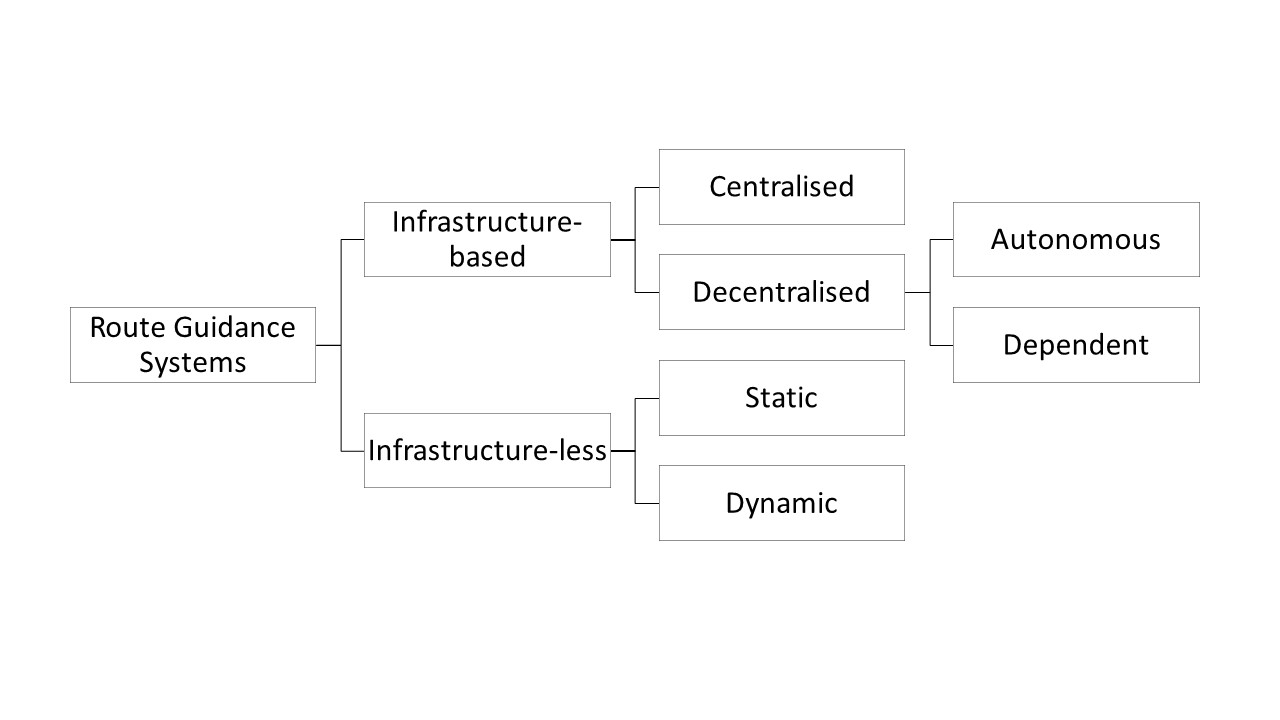
\includegraphics[width=0.55\linewidth]{image/DRS} \caption{Classification of route guidance systems (Khanjary and Hashemi, 2012)}\label{fig:unnamed-chunk-15}
\end{figure}

\textbf{Infrastrukturbasierte Architektur}
Sowohl bei \emph{zentralisierten infrastrukturbasierten Systemen} als auch bei \emph{dezentralisierten infrastrukturbasierten Systemen} werden die Daten zunächst von Verkehrserkennungssystemen erfasst und dann von Traffic Message Channel (TMC) gesammelt und extrahiert. Der Unterschied besteht darin, dass in einem \emph{zentralisierten System } die optimale Routeninformation für das gesamte Verkehrsnetz berechnet wird. Im Gegensatz dazu wird in einem \emph{abhängigen dezentralen System } die optimale Route für jedes Fahrzeug in Abhängigkeit von seinem aktuellen Standort und seinem Ziel berechnet. In einem \emph{vollständig automatisierten dezentralen System} werden die Daten von Straßenknoten gesammelt, die über das gesamte Verkehrsnetz verteilt sind und nützliche Informationen für alle umliegenden Straßen extrahieren und untereinander austauschen. Auf diese Weise kann jeder Knoten die optimalen Routen für verschiedene Ziele berechnen. Die Informationen über optimale Routen können von Fahrzeugen, Mobiltelefonen oder Wechselverkehrszeichen empfangen werden (Khanjary und Hashemi, 2012)

\textbf{Infrastrukturlose Architektur}
Das \emph{infrastrukturlose dezentrale statische System } ist eine der frühesten Entwicklungen. Die Datenbank mit der Karte des Verkehrsnetzes ist auf dem Mobiltelefon oder als fahrzeuginterne Einheit verfügbar, wobei die optimale Route auf der Grundlage statischer Informationen wie dem kürzesten Weg berechnet wird. In einem\emph{dezentralen dynamischen System }, werden Fahrzeuge (oder Mobiltelefone) zur Erfassung von Verkehrsdaten eingesetzt. Sie tauschen die Informationen untereinander über ein infrastrukturloses Protokoll wie die Kommunikation zwischen den Fahrzeugen oder Peer-to-Peer aus. Dies führt dazu, dass die Fahrzeuge über Echtzeit-Verkehrsinformationen über das gesamte Verkehrsnetz verfügen, die es ihnen ermöglichen, die optimale Route auf der Grundlage eines Ziels und der aktuellen Position des Fahrzeugs zu berechnen. Wichtig ist, dass die Genauigkeit des dynamischen Systems von der Anzahl der Fahrzeuge (oder mobilen Geräte) abhängt, die als Verkehrsdatensensoren dienen. Je mehr Fahrzeuge vorhanden sind, desto mehr Informationen können ausgetauscht werden und desto zuverlässiger sind die Daten (Khanjary und Hashemi, 2012).

\hypertarget{wichtige-interessensgruppen-13}{%
\subsection*{Wichtige Interessensgruppen}\label{wichtige-interessensgruppen-13}}
\addcontentsline{toc}{subsection}{Wichtige Interessensgruppen}

\begin{itemize}
\tightlist
\item
  \textbf{Betroffene}: Fahrer:innen
\item
  \textbf{Verantwortliche}: Lokale Regierungen, lokale oder nationale Straßeninfrastrukturanbieter, Automobilhersteller
\end{itemize}

\hypertarget{aktueller-stand-der-wissenschaft-und-forschung-13}{%
\subsection*{Aktueller Stand der Wissenschaft und Forschung}\label{aktueller-stand-der-wissenschaft-und-forschung-13}}
\addcontentsline{toc}{subsection}{Aktueller Stand der Wissenschaft und Forschung}

DRG ist bereits eine ausgereifte Technologie, daher konzentriert sich der Großteil der Forschung auf die Verbesserung verschiedener Aspekte oder die Anwendung in neuen Kontexten. In einer von Liang und Wakahara (2014) durchgeführten Studie werden beispielsweise Modelle zur Vorhersage des Stadtverkehrs vorgestellt, um ein zentrales proaktives Routenführungssystem zu schaffen. Die Ergebnisse zeigten, dass die Modelle den Vorhersagefehler verringerten und die Reisezeit verkürzten. Darüber hinaus schlugen Wang und Niu (2019) in ihrer Forschung eine simulationsbasierte verteilte dynamische Routenführung (DDRGS - Distributed Dynamic Route Guidance System) vor, die auf der Verwendung von Datenerfassungs- und Kommunikationstechniken in kooperativen Fahrzeug-Infrastruktur-Systemen (CVIS) basiert, und sie erklärten, dass die erstellte DDRGS in CVIS verwendet werden könnte. Deflorio (2003) bewertete die Leistung der Strategie zur Steuerung von DRG-Systemen in Experimenten unter der Bedingung eines schnellen Verkehrswachstums. Abschließend stellte Deflorio unter anderem fest, dass die durchschnittliche Reisezeit der DRG-Nutzer:innen in jedem untersuchten Fall kürzer war als die der Nicht-Nutzer:innen. Darüber hinaus befasst sich ein großer Teil der Forschung mit dem Einsatz von DRG im Zusammenhang mit vollständig automatisierten Fahrzeugen. In einer Studie von Lazar et al.~(2019) wird beispielsweise ein Deep Reinforcement Learning-Ansatz verwendet, um Staus im gemischten automatisierten Verkehr zu verringern. Darüber hinaus untersuchen Kaminski et al.~(2020) die Auswirkungen einer Änderung des Verbreitungsgrads von intelligenten Fahrzeugen auf die Systemeigenschaften, einschließlich der Reisezeit, in einer Umgebung, in der sowohl intelligente Fahrzeuge als auch von Menschen gesteuerte Fahrzeuge vorhanden sind. Dabei wird davon ausgegangen, dass intelligente Fahrzeuge auf Veränderungen im aktuell beobachteten Verkehr mit einer Umleitung reagieren, während herkömmliche Fahrzeuge nur auf historische Informationen zurückgreifen. Die Ergebnisse zeigen, dass der Umleitungsalgorithmus für intelligente Fahrzeuge die Gesamtreisezeit um bis zu 30\% verkürzt.

\hypertarget{aktueller-stand-der-praktischen-umsetzung-13}{%
\subsection*{Aktueller Stand der praktischen Umsetzung}\label{aktueller-stand-der-praktischen-umsetzung-13}}
\addcontentsline{toc}{subsection}{Aktueller Stand der praktischen Umsetzung}

Heutzutage nutzen Fahrer:innen verschiedener Automarken das Dynamic Route Guidance System bereits im Rahmen der dynamischen Navigation in der Fahrzeugausstattung. Seat (2012) bietet diese Funktion in der Navi-Satellitennavigationssoftware an. Seat gibt in seinem Handbuch für Autobesitzer an, dass die dynamische Routenführung auf dem TMC-Bericht basiert und die Rundfunkanstalten für diese Funktion verantwortlich sind (Media System Plus/ Navi System Owner's manual, 2012). Eine ähnliche Technologie wird auch von Volkswagen verwendet (Volkswagen, 2021). Eines der beliebtesten Tools zur Routenführung ist jedoch Google Maps, das dynamische Karten zur Verfügung stellt und Echtzeitdaten aus verschiedenen Kanälen verwendet, um die Karten so aktuell wie möglich zu halten (Custom Maps \textbar{} Google Maps Platform \textbar{} Google Cloud, 2021). Die Palette der von Google Maps angebotenen Funktionen wächst ständig. Kürzlich wurde über die reine dynamische Routenführung hinaus die Funktion ``Parkplatzsuche'' eingeführt (Vielmeier, 2019). Darüber hinaus spielt die dynamische Routenplanung eine wichtige Rolle im gewerblichen Verkehr und bei städtischen Lieferungen (PTVGroup.com, 2021).

\hypertarget{relevante-initiativen-in-uxf6sterreich-13}{%
\subsection*{Relevante Initiativen in Österreich}\label{relevante-initiativen-in-uxf6sterreich-13}}
\addcontentsline{toc}{subsection}{Relevante Initiativen in Österreich}

\begin{itemize}
\tightlist
\item
  \href{https://www.volkswagen.at/technik-lexikon/navigationssystem}{Volkswagen}
\item
  \href{https://blog.ptvgroup.com/de/stadt-und-mobilitaet/routing-engine-hyperpath/}{PTVGroup}
\item
  \href{https://www.capterra.at/directory/30944/route-planning/software}{Capterra.at}
\end{itemize}

\hypertarget{auswirkungen-in-bezug-auf-die-ziele-fuxfcr-nachhaltige-entwicklung-sdgs-13}{%
\subsection*{Auswirkungen in Bezug auf die Ziele für nachhaltige Entwicklung (SDGs)}\label{auswirkungen-in-bezug-auf-die-ziele-fuxfcr-nachhaltige-entwicklung-sdgs-13}}
\addcontentsline{toc}{subsection}{Auswirkungen in Bezug auf die Ziele für nachhaltige Entwicklung (SDGs)}

\begin{longtable}[]{@{}ccccc@{}}
\toprule
\begin{minipage}[b]{0.17\columnwidth}\centering
Ebene der Auswirkungen\strut
\end{minipage} & \begin{minipage}[b]{0.16\columnwidth}\centering
Indikator\strut
\end{minipage} & \begin{minipage}[b]{0.17\columnwidth}\centering
Richtung der Auswirkungen\strut
\end{minipage} & \begin{minipage}[b]{0.17\columnwidth}\centering
Beschreibung des Ziels \& SDG\strut
\end{minipage} & \begin{minipage}[b]{0.17\columnwidth}\centering
Quelle\strut
\end{minipage}\tabularnewline
\midrule
\endhead
\begin{minipage}[t]{0.17\columnwidth}\centering
Individuell\strut
\end{minipage} & \begin{minipage}[t]{0.16\columnwidth}\centering
Verkuerzte Reisezeit\strut
\end{minipage} & \begin{minipage}[t]{0.17\columnwidth}\centering
\textbf{+}\strut
\end{minipage} & \begin{minipage}[t]{0.17\columnwidth}\centering
Nachhaltige wirtschaftliche Entwicklung (\emph{8,11})\strut
\end{minipage} & \begin{minipage}[t]{0.17\columnwidth}\centering
Deflorio, 2003\strut
\end{minipage}\tabularnewline
\begin{minipage}[t]{0.17\columnwidth}\centering
Systemisch\strut
\end{minipage} & \begin{minipage}[t]{0.16\columnwidth}\centering
Geringeres Unfallrisiko durch Routenwechsel\strut
\end{minipage} & \begin{minipage}[t]{0.17\columnwidth}\centering
\textbf{+}\strut
\end{minipage} & \begin{minipage}[t]{0.17\columnwidth}\centering
Gesundheit und Wohlbefinden (\emph{3})\strut
\end{minipage} & \begin{minipage}[t]{0.17\columnwidth}\centering
Chatterjee and McDonald, 1999\strut
\end{minipage}\tabularnewline
\bottomrule
\end{longtable}

\hypertarget{technologie--und-gesellschaftlicher-bereitschaftsgrad-11}{%
\subsection*{Technologie- und gesellschaftlicher Bereitschaftsgrad}\label{technologie--und-gesellschaftlicher-bereitschaftsgrad-11}}
\addcontentsline{toc}{subsection}{Technologie- und gesellschaftlicher Bereitschaftsgrad}

\begin{longtable}[]{@{}cc@{}}
\toprule
Stand der Technologiebereitschaft & Gesellschaftlicher Bereitschaftsgrad\tabularnewline
\midrule
\endhead
7-9 & 8-9\tabularnewline
\bottomrule
\end{longtable}

\hypertarget{offene-fragen-13}{%
\subsection*{Offene Fragen}\label{offene-fragen-13}}
\addcontentsline{toc}{subsection}{Offene Fragen}

\begin{enumerate}
\def\labelenumi{\arabic{enumi}.}
\tightlist
\item
  Wie kann die zeitliche Genauigkeit und generell die Leistung der dynamischen Routenführung durch Verkehrsfunkkanäle verbessert werden?
\item
  Wirkt sich die dynamische Routenführung auf die Sicherheit der Fahrer:innen aus und wenn ja, in welchem Maße?
\item
  Was sind die Grenzen und welche Risiken könnten durch die dynamische Routenführung möglicherweise vermieden werden?
\item
  Wie ist die Anwendbarkeit von DRG für vollständig automatisierte Fahrzeuge?
\end{enumerate}

\hypertarget{weitere-links-11}{%
\subsection*{Weitere links}\label{weitere-links-11}}
\addcontentsline{toc}{subsection}{Weitere links}

\begin{itemize}
\tightlist
\item
  \href{https://www.verizonconnect.com/at/industrie/vertriebsroutenplaner/}{Verizonconnect.com}
\end{itemize}

\hypertarget{referenzen-13}{%
\subsection*{Referenzen}\label{referenzen-13}}
\addcontentsline{toc}{subsection}{Referenzen}

\begin{itemize}
\tightlist
\item
  Chatterjee, K. and McDonald, M., (1999). THE NETWORK SAFETY EFFECTS OF DYNAMIC ROUTE GUIDANCE. ITS Journal - Intelligent Transportation Systems Journal, 4(3-4), pp.258-260.
\item
  Blischke, F., \& Hessing, B. (1998). Dynamic Route Guidance - Different Approaches to the System Concepts. SAE Transactions, 107, 1107-1111. Available at: \url{http://www.jstor.org/stable/44741041} {[}Accessed: 22 July 2021{]}
\item
  Deflorio, F., (2003). Evaluation of a reactive dynamic route guidance strategy. Transportation Research Part C: Emerging Technologies, 11(5), pp.375-388.
\item
  European Commission. (2021). Traveller Information - Mobility and Transport - European Commission. Available at: \url{https://ec.europa.eu/transport/themes/its/road/application_areas/traveller_information_es} {[}Accessed: 23 July 2021{]}.
\item
  Fan, Y., Lu, D., Li, Y. and Jiang, F., (2010). Design scheme of Distributed Dynamic Route Guidance System. 2010 2nd International Conference on Education Technology and Computer.
\item
  Google Cloud. (2021). Custom Maps \textbar{} Google Maps Platform \textbar{} Google Cloud. Available at: \url{https://cloud.google.com/maps-platform/maps} {[}Accessed: 23 July 2021{]}.
\item
  Kaminski, B., Krainski, A., Mashatan, A., Pralat, P., \& Szufel, P. (2020). Multiagent Routing Simulation with Partial Smart Vehicles Penetration. Journal of Advanced Transportation, 2020.
\item
  Khanjary, M., \& Hashemi, S. M. (2012, May). Route guidance systems: Review and classification. In 2012 6th Euro American Conference on Telematics and Information Systems (EATIS) (pp.~1-7). IEEE.
\item
  Lazar, D. A., Biyik, E., Sadigh, D., \& Pedarsani, R. (2021). Learning how to dynamically route autonomous vehicles on shared roads. Transportation Research Part C: Emerging Technologies, 130, 103258.
\item
  Liang, Z. and Wakahara, Y., (2014). Real-time urban traffic amount prediction models for dynamic route guidance systems. EURASIP Journal on Wireless Communications and Networking, 2014(1).
\item
  Media System Plus. (2012). Media System Plus/ Navi System Owner's manual. Available at: \url{https://www.firstforseatcars.com/downloads/multimedia/media-system-plus-navi-system-owners-manual.pdf} {[}Accessed: 22 July 2021{]}.
\item
  Mobility and transport. (2021). Intelligent transport systems Traveller Information. Available at: \url{https://ec.europa.eu/transport/themes/its/road/application_areas/traveller_information_es} {[}Accessed: 22 July 2021{]}.
\item
  Park, D., Kim, H., Lee, C. and Lee, K., (2009). Location-based dynamic route guidance system of Korea: System design, algorithms and initial results. KSCE Journal of Civil Engineering, 14(1), pp.51-59.
\item
  PTVGroup.com (2021). PTV Map\&Guide - der weltweit führende Lkw Routenplaner mit Transportkosten- und Mautrechner. Available at: \url{https://www.ptvgroup.com/de/loesungen/produkte/ptv-mapandguide/} {[}Accessed: 28 July 2021{]}
\item
  Seat.com. (2021). Dynamic Route Guidance - Car Terms \textbar{} SEAT. Available at: \url{https://www.seat.com/car-terms/d/dynaminc-route-guidance.html} {[}Accessed: 23 July 2021{]}.
\item
  Wang, J. and Niu, H., (2019). A distributed dynamic route guidance approach based on short-term forecasts in cooperative infrastructure-vehicle systems. Transportation Research Part D: Transport and Environment, 66, pp.23-34.
\item
  Vielmeier J. (2019). Google Maps als Navi verwenden: Das müsst ihr beachten. Available at: \url{https://trendblog.euronics.de/mobile-web/google-maps-als-navi-verwenden-das-muesst-ihr-beachten-61614/}. {[}Accessed: 28 July 2021{]}
\item
  Volkswagen.at (2021) Navigation. Volkswagen Technik-Highlights. Available at: \url{https://www.volkswagen.at/technik-lexikon/navigationssystem} {[}Accessed: 28 July 2021{]}.
\end{itemize}

\hypertarget{variable_speed}{%
\section{Variable Geschwindigkeitsbegrenzungen und dynamisches Beschilderungssystem}\label{variable_speed}}

\hypertarget{synonyme-13}{%
\subsection*{Synonyme}\label{synonyme-13}}
\addcontentsline{toc}{subsection}{Synonyme}

\emph{Variable Geschwindigkeitsbegrenzungen (VSL - Variable speed limits), dynamische Geschwindigkeitsbegrenzungen (DSL - dynamic speed limits), Verkehrsbeeinflussungsanlagen (VBA), Wechselverkehrszeichen (CMS - Changeable Message Signs), Dynamisches Beschilderungssystem}

\hypertarget{definition-14}{%
\subsection*{Definition}\label{definition-14}}
\addcontentsline{toc}{subsection}{Definition}

Geschwindigkeitsbegrenzungen beruhen auf Sicherheits-, Mobilitäts- und Umwelterwägungen. Während feste Geschwindigkeitsbegrenzungen die angemessene Geschwindigkeit für durchschnittliche Bedingungen darstellen, berücksichtigen variable oder dynamische Geschwindigkeitsbegrenzungen (DSL) den Verkehr in Echtzeit oder die Straßen- und Wetterbedingungen. Letztere spiegeln daher die sichere Geschwindigkeit besser wider (Mobilität und Verkehr, 2020). Die Verkehrsteilnehmer:innen werden in der Regel durch elektronische Schilder über oder neben den Fahrspuren über das aktuelle Tempolimit informiert (De Pauw et al., 2018), wie in Abbildung 1 dargestellt. Diese können durch Warnschilder ergänzt werden (dynamisches Beschilderungssystem). Wenn beispielsweise die übliche Höchstgeschwindigkeit 100 km/h beträgt, könnte das DSL auf 80 km/h und weiter auf 60 km/h geändert werden, um Auffahrunfälle zu vermeiden, wenn z. B. ein Stau vorausgeht oder die Wetterbedingungen schwierig sind.

\begin{figure}
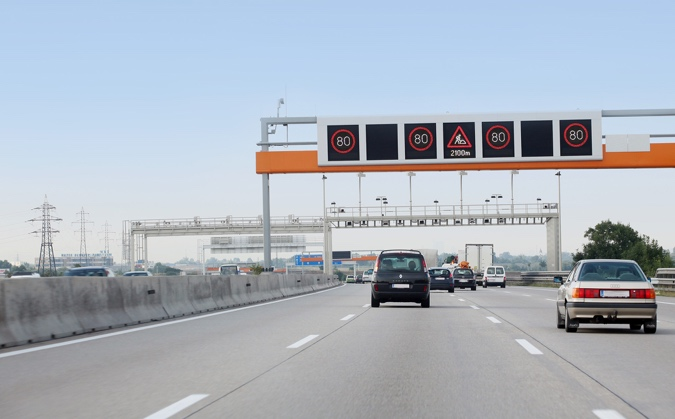
\includegraphics[width=0.9\linewidth]{image/dynamic_signage} \caption{Dynamisches Beschilderungssystem in Oesterreich (ASFiNAG, 2019b)}\label{fig:unnamed-chunk-18}
\end{figure}

Was die Auswirkungen auf die gesellschaftliche Ebene betrifft, so zeigte eine belgische Studie von E. De Pauw et al.~einen signifikanten Rückgang (-18 \%) der Zahl der Unfälle mit Verletzten nach der Einführung eines DSL-Systems (De Pauw et al., 2018). F.G. Habtemichael und L. de Picado Santos (2013) fanden heraus, dass ein DSL-System den höchsten Sicherheitsnutzen bei stark überlasteten Verkehrsbedingungen hat. Der betriebliche Nutzen wiederum war bei leicht überlasteten Verkehrsbedingungen am höchsten. Der Erfolg von DSL hängt jedoch in hohem Maße von der Einhaltung der Vorschriften durch die Fahrer:innen ab (Habtemichael \& de Picado Santos, 2013). Neben den Sicherheitsaspekten besteht das Ziel von DSL darin, den Verkehrsfluss zu harmonisieren. Starker Verkehr kann Stoßwellen verursachen, die zu längeren Fahrzeiten und großen Geschwindigkeitsschwankungen zwischen den Fahrzeugen führen. Letzteres kann wiederum zu unsicheren Situationen führen. Durch den Einsatz von DSL könnte dieses Phänomen verringert werden (Hegyi et al., 2005). Die Effizienz des Verkehrsflusses kann noch weiter verbessert werden, wenn DSL mit einer koordinierten Rampenzählung kombiniert wird (Carlson, 2010). Geschwindigkeitsbegrenzungen können auch aufgrund hoher Emissionswerte vorübergehend herabgesetzt werden. Wenn die Emissionswerte in Kombination mit dem Verkehrsaufkommen einen bestimmten Wert erreichen, reagiert das DSL-System automatisch und senkt die Geschwindigkeitsbegrenzung für eine bestimmte Zeit. Wie hoch dieses Niveau ist, hängt von den lokalen Richtlinien ab (ASFiNAG, 2019c).

\hypertarget{wichtige-interessensgruppen-14}{%
\subsection*{Wichtige Interessensgruppen}\label{wichtige-interessensgruppen-14}}
\addcontentsline{toc}{subsection}{Wichtige Interessensgruppen}

\begin{itemize}
\tightlist
\item
  \textbf{Betroffene}: Benutzer:innen von Autobahnen, Fahrer:innen
\item
  \textbf{Verantwortliche}: Autobahninfrastruktur-Agenturen, Technologie-Anbieter, politische Entscheidungsträger:innen, staatliche Behörden
\end{itemize}

\hypertarget{aktueller-stand-der-wissenschaft-und-forschung-14}{%
\subsection*{Aktueller Stand der Wissenschaft und Forschung}\label{aktueller-stand-der-wissenschaft-und-forschung-14}}
\addcontentsline{toc}{subsection}{Aktueller Stand der Wissenschaft und Forschung}

Studien zeigen, dass die meisten DSL-Einführungen in Europa rückblickend die Verkehrssicherheit und den Verkehrsfluss effizient verbessert haben. In den Vereinigten Staaten war die Erhöhung der Sicherheit ebenfalls signifikant, aber die Verbesserung des Verkehrsflusses war umstritten (Lu \& Shladover, 2014). Hassan et al.~(2012) fanden heraus, dass bei schlechten Wetterbedingungen die Kombination von Wechselverkehrszeichen (CMS) und DSL die beste Möglichkeit zur Verbesserung der Sicherheit war. Aktuelle Forschungen zeigen, dass die Vorteile von DSL-Systemen durch die Integration in eine vollständig vernetzte Fahrzeugumgebung (Wu et al., 2020) verbessert werden könnten. Derzeit konzentriert sich die Forschung auf die Integration von C-ITS, um die Infrastruktur mit den Fahrzeugen zu verbinden. In den nächsten Jahren sollten europäische Normen entwickelt werden (Erhart, 2019).

\hypertarget{aktueller-stand-der-praktischen-umsetzung-14}{%
\subsection*{Aktueller Stand der praktischen Umsetzung}\label{aktueller-stand-der-praktischen-umsetzung-14}}
\addcontentsline{toc}{subsection}{Aktueller Stand der praktischen Umsetzung}

DSL-Systeme werden auf der ganzen Welt eingeführt und verwendet. Die verwendeten Algorithmen unterscheiden sich jedoch. DSL integriert mit C-ITS wurde in einer Testumgebung implementiert (Erhart, 2019). Die österreichischen Autobahnen werden von der ASFiNAG verwaltet - derzeit sind dort 17 DSL-Systeme im Einsatz. Das bedeutet, dass etwa 19 \% des österreichischen Autobahnnetzes derzeit mit einem DSL-System ausgestattet sind (ASFiNAG, 2019a). Es gibt also noch Ausbaupotenzial. Ein Global Player im Verkehrsmanagement ist das österreichische Unternehmen Kapsch TrafficCom. Weltweit haben sie ihre Systeme auf mehr als 3.500 km Autobahn implementiert (Kapsch TrefficCom). Die rund 5.000 Mitarbeiter:innen von Kapsch TrafficCom erwirtschafteten im Wirtschaftsjahr 2018/19 einen Umsatz von 738 Millionen Euro.

\hypertarget{relevante-initiativen-in-uxf6sterreich-14}{%
\subsection*{Relevante Initiativen in Österreich}\label{relevante-initiativen-in-uxf6sterreich-14}}
\addcontentsline{toc}{subsection}{Relevante Initiativen in Österreich}

\begin{itemize}
\tightlist
\item
  \href{https://www.asfinag.at/verkehrssicherheit/verkehrsmanagement/verkehrssteuerung/}{Asfinag}
\item
  \href{https://blog.asfinag.at/technik-innovation/c-its-vernetzte-autos-intelligenter-verkehr/}{Asifinag blog}
\item
  \href{https://www.kapsch.net/ktc/Portfolio/IMS/Congestion/Highway-Traffic-Management}{kapsch.net}
\item
  \href{https://www.strabag-iss.com/databases/internet/_public/content30.nsf/web30?Openagent\&id=DE-STRABAGISS-DE_verkehrstechnik.html\&men1=3\&men2=5\&sid=351}{strabag-iss.com}
\item
  \href{https://www.pke.at/index.php?id=17\#c117}{pke.at}
\item
  \href{http://www.aigner-stahlbau.at/leistungen/verkehrstechnik/}{aigner-stahlbau.at}
\end{itemize}

\hypertarget{auswirkungen-in-bezug-auf-die-ziele-fuxfcr-nachhaltige-entwicklung-sdgs-14}{%
\subsection*{Auswirkungen in Bezug auf die Ziele für nachhaltige Entwicklung (SDGs)}\label{auswirkungen-in-bezug-auf-die-ziele-fuxfcr-nachhaltige-entwicklung-sdgs-14}}
\addcontentsline{toc}{subsection}{Auswirkungen in Bezug auf die Ziele für nachhaltige Entwicklung (SDGs)}

\begin{longtable}[]{@{}ccccc@{}}
\toprule
\begin{minipage}[b]{0.17\columnwidth}\centering
Ebene der Auswirkungen\strut
\end{minipage} & \begin{minipage}[b]{0.16\columnwidth}\centering
Indikator\strut
\end{minipage} & \begin{minipage}[b]{0.17\columnwidth}\centering
Richtung der Auswirkungen\strut
\end{minipage} & \begin{minipage}[b]{0.17\columnwidth}\centering
Beschreibung des Ziels \& SDG\strut
\end{minipage} & \begin{minipage}[b]{0.17\columnwidth}\centering
Quelle\strut
\end{minipage}\tabularnewline
\midrule
\endhead
\begin{minipage}[t]{0.17\columnwidth}\centering
Individuell\strut
\end{minipage} & \begin{minipage}[t]{0.16\columnwidth}\centering
Toedliche Kollisionen reduziert\strut
\end{minipage} & \begin{minipage}[t]{0.17\columnwidth}\centering
\textbf{+}\strut
\end{minipage} & \begin{minipage}[t]{0.17\columnwidth}\centering
Gesundheit und Wohlbefinden (\emph{3})\strut
\end{minipage} & \begin{minipage}[t]{0.17\columnwidth}\centering
Hegyi et al., 2005\strut
\end{minipage}\tabularnewline
\begin{minipage}[t]{0.17\columnwidth}\centering
Individuell\strut
\end{minipage} & \begin{minipage}[t]{0.16\columnwidth}\centering
Verkuerzte Reisezeit\strut
\end{minipage} & \begin{minipage}[t]{0.17\columnwidth}\centering
\textbf{+}\strut
\end{minipage} & \begin{minipage}[t]{0.17\columnwidth}\centering
Nachhaltige wirtschaftliche Entwicklung (\emph{8,11})\strut
\end{minipage} & \begin{minipage}[t]{0.17\columnwidth}\centering
Habtemichael \& de Picado Santos, 2013\strut
\end{minipage}\tabularnewline
\begin{minipage}[t]{0.17\columnwidth}\centering
Systemisch\strut
\end{minipage} & \begin{minipage}[t]{0.16\columnwidth}\centering
Toedliche Kollisionen reduziert\strut
\end{minipage} & \begin{minipage}[t]{0.17\columnwidth}\centering
\textbf{+}\strut
\end{minipage} & \begin{minipage}[t]{0.17\columnwidth}\centering
Gesundheit und Wohlbefinden (\emph{3})\strut
\end{minipage} & \begin{minipage}[t]{0.17\columnwidth}\centering
Hegyi et al., 2005\strut
\end{minipage}\tabularnewline
\begin{minipage}[t]{0.17\columnwidth}\centering
Systemisch\strut
\end{minipage} & \begin{minipage}[t]{0.16\columnwidth}\centering
Jaehrlicher Rueckgang der Treibhausgasemissionen\strut
\end{minipage} & \begin{minipage}[t]{0.17\columnwidth}\centering
\textbf{+}\strut
\end{minipage} & \begin{minipage}[t]{0.17\columnwidth}\centering
Oekologische Nachhaltigkeit (\emph{7,12-13,15})\strut
\end{minipage} & \begin{minipage}[t]{0.17\columnwidth}\centering
Schimany, 2011\strut
\end{minipage}\tabularnewline
\bottomrule
\end{longtable}

\hypertarget{technologie--und-gesellschaftlicher-bereitschaftsgrad-12}{%
\subsection*{Technologie- und gesellschaftlicher Bereitschaftsgrad}\label{technologie--und-gesellschaftlicher-bereitschaftsgrad-12}}
\addcontentsline{toc}{subsection}{Technologie- und gesellschaftlicher Bereitschaftsgrad}

\begin{longtable}[]{@{}cc@{}}
\toprule
Stand der Technologiebereitschaft & Gesellschaftlicher Bereitschaftsgrad\tabularnewline
\midrule
\endhead
7-9 & 8-9\tabularnewline
\bottomrule
\end{longtable}

\hypertarget{offene-fragen-14}{%
\subsection*{Offene Fragen}\label{offene-fragen-14}}
\addcontentsline{toc}{subsection}{Offene Fragen}

\begin{enumerate}
\def\labelenumi{\arabic{enumi}.}
\tightlist
\item
  Welche Algorithmen für DSL sind die effizientesten?
\item
  Wie kann DSL weiter entwickelt werden?
\item
  Wie kann der ausfallsichere Betrieb verbessert werden?
\item
  Wie kann DSL mit C-ITS kombiniert werden?
\end{enumerate}

\hypertarget{referenzen-14}{%
\subsection*{Referenzen}\label{referenzen-14}}
\addcontentsline{toc}{subsection}{Referenzen}

\begin{itemize}
\tightlist
\item
  ASFiNAG. (2019a). Handlungsfelder. Available at: \url{http://verkehrssicherheit.asfinag.at/aktionsprogramme/handlungsfelder/} {[}Accessed: 17 December 2020{]}.
\item
  ASFiNAG. (2019b). Verkehrsbeeinflussungsanlagen - Für mehr Sicherheit: Arten von Verkehrsbeeinflussungsanlagen. Available at: \url{https://asfinag.azureedge.net/media/1607/vba-fotomontage.jpg} {[}Accessed: 11 December 2020{]}.
\item
  ASFiNAG. (2019c). Verkehrsbeeinflussungsanlagen - Für mehr Sicherheit: Die VBA und der ``Lufthunderter''. Available at: \url{https://www.asfinag.at/verkehrssicherheit/verkehrsmanagement/verkehrssteuerung/} {[}Accessed: 3 December 2020{]}.
\item
  Carlson, R. C., Papamichail, I., Papageorgiou, M., \& Messmer, A. (2010). Optimal motorway traffic flow control involving variable speed limits and ramp metering. Transportation Science, 44(2), 238-253.
\item
  De Pauw, E., Daniels, S., Franckx, L., \& Mayeres, I. (2018). Safety effects of dynamic speed limits on motorways. Accident Analysis \& Prevention, 114, 83-89.
\item
  Erhart, Jaqueline. (2019). Vernetzte Autos, intelligenter Verkehr: Was C-ITS ist, was es kann und wem es nutzt. Available at: \url{https://blog.asfinag.at/technik-innovation/c-its-vernetzte-autos-intelligenter-verkehr/} {[}Accessed: 17 December 2020{]}.
\item
  Habtemichael, F. G., \& de Picado Santos, L. (2013). Safety and Operational Benefits of Variable Speed Limits under Different Traffic Conditions and Driver Compliance Levels. Transportation Research Record, 2386(1), 7-15. \url{https://doi.org/10.3141/2386-02}
\item
  Hassan, H. M., Abdel-Aty, M. A., Choi, K., \& Algadhi, S. A. (2012). Driver behavior and preferences for changeable message signs and variable speed limits in reduced visibility conditions. Journal of Intelligent Transportation Systems, 16(3), 132-146.
\item
  Hegyi, A., De Schutter, B., \& Hellendoorn, J. (2005). Optimal coordination of variable speed limits to suppress shock waves. IEEE Transactions on intelligent transportation systems, 6(1), 102-112.
\item
  Kapsch TrefficCom. Verkehrsmanagement auf Autobahnen. Available at: \url{https://www.kapsch.net/ktc/Portfolio/IMS/Congestion/Highway-Traffic-Management}
\item
  Lu, X.-Y., \& Shladover, S. E. (2014). Review of Variable Speed Limits and Advisories: Theory, Algorithms, and Practice. Transportation Research Record, 2423(1), 15-23. \url{https://doi.org/10.3141/2423-03} {[}Accessed: 8 January 2021{]}
\item
  Mobility and Transport \textbar{} European Commission. (2020). Dynamic speed limits. Available at: \url{https://ec.europa.eu/transport/road_safety/specialist/knowledge/speed/new_technologies_new_opportunities/dynamic_speed_limits_en} {[}Accessed: 2 December 2020{]}.
\item
  Schimany, H. K. (2011). Blue Globe Foresight.
\item
  Wu, Y., Abdel-Aty, M., Wang, L., \& Rahman, M. S. (2020). Combined connected vehicles and variable speed limit strategies to reduce rear-end crash risk under fog conditions. Journal of Intelligent Transportation Systems, 24(5), 494-513.
\end{itemize}

\hypertarget{adaptive_traffic_control}{%
\section{Intelligente Verkehrssignalsteuerung}\label{adaptive_traffic_control}}

\hypertarget{synonyme-14}{%
\subsection*{Synonyme}\label{synonyme-14}}
\addcontentsline{toc}{subsection}{Synonyme}

\emph{Intelligente Ampelanlagen, adaptive Verkehrssignalsteuerung (ATSC - Adaptive Traffic Signal Control), Verkehrssignalsteuerung (TST - Traffic Signal Timing), Verkehrssignalsteuerung (TSC - Traffic Signal Control)}

\hypertarget{definition-15}{%
\subsection*{Definition}\label{definition-15}}
\addcontentsline{toc}{subsection}{Definition}

In den letzten Jahren haben die steigende Bevölkerungszahl und der dringende Bedarf an effizientem Verkehr zu schwerwiegenden Verkehrsproblemen geführt, insbesondere in städtischen Gebieten. Es wurden Lösungen zur Stauabschwächung vorgeschlagen, wie z. B. die Optimierung des Straßennetzes und die Verbesserung grundlegender städtischer Verwaltungseinrichtungen, um den durch die großen Verkehrsströme während der Spitzenzeiten verursachten Druck zu bewältigen. Unter allen möglichen Methoden hat sich die adaptive Verkehrssignalsteuerung (ATSC), bei der die Intelligenz in die Ampelsteuerungssysteme integriert wird, als wirtschaftlich und effizient erwiesen, um den Verkehrsdruck an überlasteten Kreuzungen zu verringern. Mit der Entwicklung von Deep-Learning-Techniken haben ATSC-Strategien großes Potenzial für die Integration modernster intelligenter Methoden gezeigt (Wang et al., 2021).
Bestehende Ampelsteuerungssysteme verwenden entweder feste Programme ohne Berücksichtigung des Echtzeitverkehrs oder berücksichtigen den Verkehr kaum (Casas, 2017). Sie stellen die Ampeln entweder in jedem Zyklus auf die gleiche Dauer ein oder variieren die Dauer in Abhängigkeit von historischen Informationen. Einige von ihnen verwenden Eingangsdaten von unterirdischen Sensoren, wie z. B. Induktionsschleifendetektoren, um Fahrzeuge in der Nähe der Ampel zu erkennen. Diese Daten werden jedoch nur sehr grob verarbeitet, um die Dauer von grünen und roten Ampeln zu bestimmen. Folglich funktionieren sie in einigen Fällen (mit geringer Effizienz); bei Ereignissen wie Sportveranstaltungen, Festivals, Wetterbedingungen oder einem typischen Szenario mit hohem Verkehrsaufkommen neigen die bestehenden Kontrollsysteme jedoch dazu, lahmgelegt zu werden.
In einer aktuellen Forschungsarbeit von Liang et al.~(2019) wird berichtet, dass erfahrene Polizeibeamt:innen eine Kreuzung effizient und direkt durch Winken kontrollieren können. Insbesondere in Szenarien mit hohem Verkehrsaufkommen beobachten menschliche Bediener:innen die Echtzeit-Verkehrsbedingungen an den kreuzenden Straßen und passen die Dauer der Durchfahrtszeit entsprechend an. Das Ziel der adaptiven Verkehrssignalsteuerung ist es, durch den Einsatz von V2X und Deep Reinforcement Learning (Wang et al., 2021) eine Flexibilität und Effizienz im Verkehrsmanagement zu erreichen, das mit dem von menschlichen Bediener:innen vergleichbar ist.

\hypertarget{wichtige-interessensgruppen-15}{%
\subsection*{Wichtige Interessensgruppen}\label{wichtige-interessensgruppen-15}}
\addcontentsline{toc}{subsection}{Wichtige Interessensgruppen}

\begin{itemize}
\tightlist
\item
  \textbf{Betroffene}: Autofahrer:innen, Radfahrer:innen, Fußgänger:innen
\item
  \textbf{Verantwortliche}: Lokale Regierungen, lokale oder nationale Straßeninfrastrukturanbieter, Automobilhersteller
\end{itemize}

\hypertarget{aktueller-stand-der-wissenschaft-und-forschung-15}{%
\subsection*{Aktueller Stand der Wissenschaft und Forschung}\label{aktueller-stand-der-wissenschaft-und-forschung-15}}
\addcontentsline{toc}{subsection}{Aktueller Stand der Wissenschaft und Forschung}

Bestehende ATSC-Methoden konzentrieren sich darauf, die Dauer von Grün- oder Rotphasen auf der Grundlage von Echtzeitinformationen zu variieren. Dieser Ansatz ist jedoch nicht optimal, da er die Auswirkungen der aktuellen Dauer der grünen und roten Ampeln auf den nachfolgenden Verkehr vernachlässigt. Daher schneidet ATSC besser ab als das System mit fester Dauer, aber schlechter als flexiblere Methoden, da die optimale Phasendauer in den letzten Zyklen unter Berücksichtigung aktueller Informationen über komplexe Verkehrsbedingungen in der Zukunft nicht besser ist.

Mit Deep Learning (DL)-Methoden (die als Input für die Kreuzungssteuerung dienen) kann die optimale Gestaltung der grundlegenden Steuerungsindizes wie Grünphasendauer und Phasenfolge der Ampel an einer Kreuzung als ein optimales Entscheidungsverfahren betrachtet werden. Anschließend wird das Reinforcement Learning (RL) auf die Signalsteuerung angewandt, um das beste Steuerungsverfahren für eine signalisierte Kreuzung zu finden. Um jedoch eine sofortige Datenerfassung und -übertragung mit geringer Latenzzeit zu erreichen, ist ein kooperatives Fahrzeuginfrastruktursystem (CVIS) erforderlich, das die Kommunikation zwischen den Fahrzeugen und zwischen Fahrzeugen und straßenseitiger Infrastruktur unterstützt (siehe \protect\hyperlink{v2x}{Abschnitt V2X}). Im Vergleich zu herkömmlichen Sensordetektoren kann V2X genauere Verkehrsdaten sammeln, um umfassende Informationen für die Verkehrssteuerung zu liefern, was zu besseren RL-Entscheidungen führt (Wang et al., 2021)
Darüber hinaus ergab die Analyse der neueren Literatur zur Optimierung von TSC-Systemen, die von Januar 2015 bis Januar 2020 veröffentlicht wurden, dass sich nur zwei Arbeiten mit signalisierten Kreisverkehren befassen. Kreisverkehre haben eine andere Verkehrsdynamik als reguläre Kreuzungen. Angesichts des zunehmenden Einsatzes von signalisierten Kreisverkehren, insbesondere in städtischen Gebieten, wird davon ausgegangen, dass TSC für signalisierte Kreisverkehre eine besondere Forschungslücke in diesem Bereich darstellt. Obwohl es Studien gibt, die mit realen Daten und Echtzeitsteuerung durchgeführt wurden, gibt es nur wenige Ergebnisse und/oder Methoden, die in der Praxis angewandt oder angepasst wurden. Eine der größten Herausforderungen für die Forscher:innen auf diesem Gebiet besteht darin, diese Methoden den Entscheidungsträger:innen und Umsetzer:innen näher zu bringen.
Darüber hinaus befasst sich die überwiegende Mehrheit der zu diesem Thema gefundenen Arbeiten mit der zeitlichen Steuerung von Verkehrssignalen und deren Auswirkungen auf die durchschnittliche Verspätung und/oder die Emissionen. Ein wichtiger Bestandteil von stark befahrenen Kreuzungen, insbesondere in Ballungsgebieten, ist der Fußgängerverkehr. Mit Ausnahme von Vilarinho et al., (2017) und Yu et al., (2017) werden Fußgänger:innen und die Auswirkungen ihres Verhaltens in den Studien nicht modelliert. Das Gleiche gilt für das Verhalten der Fahrer:innen. Eine wichtige Forschungsrichtung wäre es, die Auswirkungen des Fußgänger- und Fahrerverhaltens auf die Modelle zu analysieren.
Außerdem nimmt die Zahl der Studien, die sich mit automatisierten Fahrzeugen und Technologien befassen, rasch zu. Die jüngsten Studien befassen sich mit der allgemeinen Frage, wie vollständig automatisierte Fahrzeuge sicher und/oder effizient und/oder umweltfreundlich in den Verkehrsfluss eingeführt werden können (Qadri et al., 2020a).
Das Lernen durch Versuch und Irrtum ist zwar der Kerngedanke von RL, aber die Lernkosten von RL für komplizierte Probleme könnten inakzeptabel sein. Daher ist die Frage, wie man effizient lernt (z. B. aus begrenzten Datenproben, effiziente Exploration, Übertragung von gelerntem Wissen), ein entscheidender Punkt für die Anwendung von RL in der Verkehrssignalsteuerung (Wei et al., 2019).

\hypertarget{aktueller-stand-der-praktischen-umsetzung-15}{%
\subsection*{Aktueller Stand der praktischen Umsetzung}\label{aktueller-stand-der-praktischen-umsetzung-15}}
\addcontentsline{toc}{subsection}{Aktueller Stand der praktischen Umsetzung}

Eine Reihe von Akteuren konzentriert sich auf die Entwicklung adaptiver Verkehrssteuerungssysteme, die eine Reihe von Smart-City-Verkehrsanwendungen unterstützen, wie z. B. Signalpriorität für öffentliche Verkehrsmittel (siehe \protect\hyperlink{public_trans_priority}{Abschnitt PTSP} für weitere Einzelheiten), Unterstützung für umweltbewusstes Fahren, Nachrichtenübermittlung, intelligente Verkehrssignalsteuerung (STSC) und Signalpräemption für Einsatzfahrzeuge (EVSP). Aufgrund dieser Faktoren und stetiger Fortschritte bei Sensoren, künstlicher Intelligenz (KI) und maschinellem Lernen wird der globale Markt für adaptive Verkehrssteuerungssysteme bis Ende 2030 voraussichtlich einen Wert von 21,9 Milliarden US-Dollar erreichen. Regierungen und Stadtverwaltungen in verschiedenen Regionen der Welt suchen nach neuen Wegen, um auf die steigende Zahl von Verkehrsunfällen und die Bewältigung von Straßenstaus zu reagieren, weshalb adaptive Verkehrssteuerungssysteme in den letzten Jahren als praktikable Alternative zur Bewältigung der bestehenden Herausforderungen auf großes Interesse gestoßen sind (The Sentinel Newspaper, 2021). Es gibt bereits zahlreiche Optionen, und weitere befinden sich noch in der Entwicklung. Zu den derzeit verfügbaren adaptiven Signalsteuerungstechnologien gehören:
- Split Cycle Offset Optimisation Technique (SCOOT);
- Sydney Coordinated Adaptive Traffic System (SCATS),
- Real Time Hierarchical Optimised Distributed Effective System (RHODES);
- Optimised Policies for Adaptive Control (OPAC) \emph{Virtual Fixed Cycle}
- ACS Lite
Echtzeit-Verkehrssteuerungssysteme haben ihre Leistungsfähigkeit unter Beweis gestellt, dennoch wurden diese Systeme bei weniger als 1 \% der bestehenden Verkehrssignale in Amerika eingesetzt. Die Federal Highway Administration arbeitet nun daran, diese Technologien auch im Rest des Landes einzuführen (Curtis, 2017). Darüber hinaus wurde beispielsweise in Deutschland das adaptive Signalsteuerungssystem auf einer 6 km langen Ausfallstraße in Münster installiert, wo es sich nachweislich positiv auf die Verkehrsqualität auswirkt und den Bustransit auf der Grundlage des angenommenen Leistungsindex um 30 \% verbessert (Brilon \& Wietholt, 2013).

\hypertarget{relevante-initiativen-in-uxf6sterreich-15}{%
\subsection*{Relevante Initiativen in Österreich}\label{relevante-initiativen-in-uxf6sterreich-15}}
\addcontentsline{toc}{subsection}{Relevante Initiativen in Österreich}

\begin{itemize}
\tightlist
\item
  \href{https://www.asfinag.at/road-safety/traffic-management/traffic-control/}{Asfinag}
\item
  \href{https://www.atc.or.at/smart-cities/smart-mobility/urban-traffic-management-solutions/}{ATC}
\end{itemize}

\hypertarget{auswirkungen-in-bezug-auf-die-ziele-fuxfcr-nachhaltige-entwicklung-sdgs-15}{%
\subsection*{Auswirkungen in Bezug auf die Ziele für nachhaltige Entwicklung (SDGs)}\label{auswirkungen-in-bezug-auf-die-ziele-fuxfcr-nachhaltige-entwicklung-sdgs-15}}
\addcontentsline{toc}{subsection}{Auswirkungen in Bezug auf die Ziele für nachhaltige Entwicklung (SDGs)}

\begin{longtable}[]{@{}ccccc@{}}
\toprule
\begin{minipage}[b]{0.17\columnwidth}\centering
Ebene der Auswirkungen\strut
\end{minipage} & \begin{minipage}[b]{0.16\columnwidth}\centering
Indikator\strut
\end{minipage} & \begin{minipage}[b]{0.17\columnwidth}\centering
Richtung der Auswirkungen\strut
\end{minipage} & \begin{minipage}[b]{0.17\columnwidth}\centering
Beschreibung des Ziels \& SDG\strut
\end{minipage} & \begin{minipage}[b]{0.17\columnwidth}\centering
Quelle\strut
\end{minipage}\tabularnewline
\midrule
\endhead
\begin{minipage}[t]{0.17\columnwidth}\centering
Systemisch\strut
\end{minipage} & \begin{minipage}[t]{0.16\columnwidth}\centering
Kaum Studien, die die Auswirkungen des Verhaltens von Fussgaenger:innen beruecksichtigen\strut
\end{minipage} & \begin{minipage}[t]{0.17\columnwidth}\centering
\textbf{-}\strut
\end{minipage} & \begin{minipage}[t]{0.17\columnwidth}\centering
Gleichheit (\emph{5,10})\strut
\end{minipage} & \begin{minipage}[t]{0.17\columnwidth}\centering
Qadri et al., 2020b\strut
\end{minipage}\tabularnewline
\begin{minipage}[t]{0.17\columnwidth}\centering
Systemisch\strut
\end{minipage} & \begin{minipage}[t]{0.16\columnwidth}\centering
Verringerung der Verkehrsueberlastung an den Kreuzungen\strut
\end{minipage} & \begin{minipage}[t]{0.17\columnwidth}\centering
\textbf{+}\strut
\end{minipage} & \begin{minipage}[t]{0.17\columnwidth}\centering
Nachhaltige wirtschaftliche Entwicklung (\emph{8,11})\strut
\end{minipage} & \begin{minipage}[t]{0.17\columnwidth}\centering
Wang et al., 2021\strut
\end{minipage}\tabularnewline
\begin{minipage}[t]{0.17\columnwidth}\centering
Systemisch\strut
\end{minipage} & \begin{minipage}[t]{0.16\columnwidth}\centering
Fortschritte bei der Nutzung von RL-Algorithmen und V2X-Technologien\strut
\end{minipage} & \begin{minipage}[t]{0.17\columnwidth}\centering
\textbf{+}\strut
\end{minipage} & \begin{minipage}[t]{0.17\columnwidth}\centering
Innovation und Infrastruktur (\emph{9})\strut
\end{minipage} & \begin{minipage}[t]{0.17\columnwidth}\centering
Wang et al., 2021\strut
\end{minipage}\tabularnewline
\bottomrule
\end{longtable}

\hypertarget{technologie--und-gesellschaftlicher-bereitschaftsgrad-13}{%
\subsection*{Technologie- und gesellschaftlicher Bereitschaftsgrad}\label{technologie--und-gesellschaftlicher-bereitschaftsgrad-13}}
\addcontentsline{toc}{subsection}{Technologie- und gesellschaftlicher Bereitschaftsgrad}

\begin{longtable}[]{@{}cc@{}}
\toprule
Stand der Technologiebereitschaft & Gesellschaftlicher Bereitschaftsgrad\tabularnewline
\midrule
\endhead
7-9 & 7-8\tabularnewline
\bottomrule
\end{longtable}

\hypertarget{offene-fragen-15}{%
\subsection*{Offene Fragen}\label{offene-fragen-15}}
\addcontentsline{toc}{subsection}{Offene Fragen}

\begin{enumerate}
\def\labelenumi{\arabic{enumi}.}
\tightlist
\item
  Wie kann ATSC für signalisierte Kreisverkehre konzipiert, entwickelt und umgesetzt werden?
\item
  Wie kann die Fußgängerbewegung in größerem Umfang in die Algorithmen von ATSC einbezogen werden?
\item
  Wie können Algorithmen des verstärkten Lernens effizient aus begrenzten Datenproben für die Steuerung von Verkehrssignalen lernen?
\end{enumerate}

\hypertarget{weitere-links-12}{%
\subsection*{Weitere links}\label{weitere-links-12}}
\addcontentsline{toc}{subsection}{Weitere links}

\begin{itemize}
\tightlist
\item
  \href{https://www.rapidflowtech.com/surtrac}{rapidflowtech.com}
\item
  \href{https://www.fhwa.dot.gov/innovation/everydaycounts/edc-1/asct.cfm}{fhwa.dot.gov}
\end{itemize}

\hypertarget{referenzen-15}{%
\subsection*{Referenzen}\label{referenzen-15}}
\addcontentsline{toc}{subsection}{Referenzen}

\begin{itemize}
\tightlist
\item
  Brilon, W., \& Wietholt, T. (2013). Experiences with adaptive signal control in Germany. Transportation research record, 2356(1), 9-16.
\item
  Casas, N. (2017). Deep deterministic policy gradient for urban traffic light control. ArXiv, 1-12.
\item
  Curtis, E. (2017, September 8). EDC-1: Adaptive Signal Control Technology \textbar{} Federal Highway Administration. \url{https://www.fhwa.dot.gov/innovation/everydaycounts/edc-1/asct.cfm}
\item
  Liang, X., Du, X., Wang, G., \& Han, Z. (2019). A Deep Reinforcement Learning Network for Traffic Light Cycle Control. IEEE Transactions on Vehicular Technology, 68(2), 1243-1253. \url{https://doi.org/10.1109/TVT.2018.2890726}
\item
  Qadri, S. S. S. M., Gökce, M. A., \& Öner, E. (2020a). State-of-art review of traffic signal control methods: challenges and opportunities. European Transport Research Review, 12(1), 55. \url{https://doi.org/10.1186/s12544-020-00439-1}
\item
  Qadri, S. S. S. M., Gökce, M. A., \& Öner, E. (2020b). State-of-art review of traffic signal control methods: challenges and opportunities. European Transport Research Review, 12(1), 1-23. \url{https://doi.org/10.1186/s12544-020-00439-1}
\item
  The Sentinel Newspaper. (2021, March 3). Adaptive Traffic Control System Market to reach US\$ 21.9 Bn by 2030 - KSU \textbar{} The Sentinel Newspaper. \url{https://ksusentinel.com/2021/03/03/adaptive-traffic-control-system-market-to-reach-us-21-9-bn-by-2030/}
\item
  Vilarinho, C., Tavares, J. P., \& Rossetti, R. J. F. (2017). Intelligent Traffic Lights: Green Time Period Negotiaton. Transportation Research Procedia, 22, 325-334. \url{https://doi.org/https://doi.org/10.1016/j.trpro.2017.03.039}
\item
  Wang, T., Cao, J., \& Hussain, A. (2021). Adaptive Traffic Signal Control for large-scale scenario with Cooperative Group-based Multi-agent reinforcement learning. Transportation Research Part C: Emerging Technologies, 125(February), 103046. \url{https://doi.org/10.1016/j.trc.2021.103046}
\item
  Wei, H., Zheng, G., Gayah, V., \& Li, Z. (2019). A survey on traffic signal control methods. ArXiv, 1(1).
\item
  Yu, C., Ma, W., Han, K., \& Yang, X. (2017). Optimization of vehicle and pedestrian signals at isolated intersections. Transportation Research Part B: Methodological, 98, 135-153. \url{https://doi.org/https://doi.org/10.1016/j.trb.2016.12.015}
\end{itemize}

\hypertarget{p_g_fleet_management}{%
\section{Flottenmanagement für Personentransport und Gütertransport}\label{p_g_fleet_management}}

\hypertarget{definition-16}{%
\subsection*{Definition}\label{definition-16}}
\addcontentsline{toc}{subsection}{Definition}

Laut Mixtelematics.com (2021) bezieht sich Fuhrparkmanagement auf die allgemeinen Maßnahmen, die ergriffen werden, um einen Fuhrpark effizient, pünktlich und innerhalb des Budgets am Laufen zu halten. Es kann definiert werden als die Prozesse, die von Fuhrparkmanager:innenn genutzt werden, um Fuhrparkaktivitäten zu überwachen und Entscheidungen zu treffen, von der Vermögensverwaltung über die Disposition, die Zeitplanung, die Routenplanung bis hin zum Erwerb und der Entsorgung von Fahrzeugen. Es hilft Unternehmen, die Einhaltung von Vorschriften zu gewährleisten, die Effizienz zu verbessern und Kosten zu senken. Es soll für Organisationen und Firmen gelten, die mehr als fünf Fahrzeuge einsetzen. Die Hauptaufgaben von Fuhrparkleitern sind Kostenreduzierung, Fahrzeugverfolgung und -sicherheit, Fahrersicherheit und -bindung, Fahrzeugbeschaffung und Einhaltung der Vorschriften für elektronische Fahrtenschreiber (ELD) (im Falle der USA). Zu den Vorteilen des Flottenmanagements gehören die Automatisierung manueller Aufgaben, die Steigerung der Rentabilität, die Verbesserung der Flottensicherheit und des Kundendienstes. Die größten Herausforderungen für Flottenmanager:innen sind Kraftstoffmanagement, Fahrzeugbeschaffung, Optimierung der Fahrzeugleistung, Einhaltung von Vorschriften, Kostenkontrolle sowie Gesundheit und Sicherheit (Mixtelematics.com, 2021).
Das Fuhrparkmanagement ist in einer Reihe von Branchen vertreten, darunter der öffentliche Verkehr, Notdienste, Transport und Vertrieb oder Vermietung und Leasing von Fahrzeugen.

\textbf{Öffentlicher Verkehr}
Das Flottenmanagement im öffentlichen Verkehr konzentriert sich auf die Überwachung und das Management von Fahrer:innen und Fahrzeugen, um den Betreibern des öffentlichen Verkehrs zu helfen, die Leistung und die Systemfähigkeit zu verbessern. Erreicht werden kann dies durch die Echtzeitverfolgung des Fahrzeugstandorts und eine zuverlässige Datenerfassung. Die Funktionen des Fahrgastflottenmanagements umfassen (Nec.com, 2021):
- Echtzeit-Fahrgastinformationssystem, bei dem der Schlüssel eine geschätzte Ankunftszeit (ETA) auf der Grundlage von Tag, Uhrzeit, Streckentyp, Fahrplantyp, Verweildauer, Reisezeit usw. ist (weitere Informationen siehe Multimodale Informationen und Routenplanung)
- Ein visuelles und akustisches Fahrgastinformationssystem im Fahrzeug wird für jede Strecke und Haltestelle definiert, das Echtzeitinformationen über den Fortschritt des Fahrzeugs, eventuelle Streckenunterbrechungen und Abweichungen liefert.
- Echtzeit-Datenanalyse und -Management überwacht die Transitdienste, einschließlich der Einhaltung von Fahrplänen und Wartezeiten.
- Routing und Fahrtenzuweisung plant Fahrten, ermöglicht aber auch eine dynamische Fahrtenzuweisung

\textbf{Transport und Verteilung}
In der Transportbranche kann die Implementierung eines Flottenmanagements durch eine mobile On-Board-Technologie bei der Routenoptimierung, der verbesserten Kommunikation mit den Fahrer:innen, dem Management des Kraftstoffverbrauchs und der effizienteren Zuweisung und Planung von Aufträgen helfen. Ein Sonderfall des Flottenmanagements sind zukünftige Flotten von AVs, wie von Hyland \& Mahmassani (2017) beschrieben, die eine umfassende Taxonomie für das Flottenmanagement von gemeinsam genutzten automatisierten Fahrzeugen liefern.

\hypertarget{wichtige-interessensgruppen-16}{%
\subsection*{Wichtige Interessensgruppen}\label{wichtige-interessensgruppen-16}}
\addcontentsline{toc}{subsection}{Wichtige Interessensgruppen}

\begin{itemize}
\tightlist
\item
  \textbf{Betroffene}: Gewerbliche Fahrer:innen, Fahrer:innen und Manager:innen öffentlicher Verkehrsmittel, Fahrgäste öffentlicher Verkehrsmittel
\item
  \textbf{Verantwortliche}: Betreiber öffentlicher Verkehrsmittel, Transportunternehmen, Fahrzeughersteller
\end{itemize}

\hypertarget{aktueller-stand-der-wissenschaft-und-forschung-16}{%
\subsection*{Aktueller Stand der Wissenschaft und Forschung}\label{aktueller-stand-der-wissenschaft-und-forschung-16}}
\addcontentsline{toc}{subsection}{Aktueller Stand der Wissenschaft und Forschung}

Die Forschung im Bereich des Flottenmanagements konzentriert sich auf die Entwicklung und Umsetzung moderner und ganzheitlicher Lösungen, die beispielsweise das Internet der Dinge (IoT) nutzen. So schlugen Killeen et al.~(2019) die Nutzung von Daten aus dem IoT im Rahmen des Flottenmanagements vor, um die vorausschauende Wartung von Flotten zu verbessern. Außerdem entwickelten Nuhic et al.~(2018) einen neuen Algorithmus zur Überwachung des Batteriezustands, um die Genauigkeit der Vorhersage der Batterieabnutzung zu erhöhen. Stancel \& Surugiu (2017) entwickelten ein System, das LKW-Züge in Echtzeit überwacht und Informationen über die Länge der Route, die Fahrzeit und den Kraftstoffverbrauch liefert. Das System ermöglicht die Berechnung optimaler Routen im Hinblick auf den Kraftstoffverbrauch.

\hypertarget{aktueller-stand-der-praktischen-umsetzung-16}{%
\subsection*{Aktueller Stand der praktischen Umsetzung}\label{aktueller-stand-der-praktischen-umsetzung-16}}
\addcontentsline{toc}{subsection}{Aktueller Stand der praktischen Umsetzung}

Derzeit bieten mehrere technologieorientierte Unternehmen wie \href{https://www.fleetio.com/}{Fleetio}, \href{https://www.samsara.com/at/}{Sesmara}, \href{https://gsmtasks.com/}{GSMtasks} oder \href{https://www.avrios.com/?utm_source=capterra\&utm_medium=cpc\&utm_campaign=software-comparison}{Avrios} weltweit Software für das Flottenmanagement an. Es gibt auch Unternehmen wie \href{https://www.urbantz.com/}{Urbantz} oder \href{https://onfleet.com/}{OnFleet} die sich auf die Verwaltung lokaler, umweltfreundlicher Lieferungen auf der letzten Meile spezialisiert haben. Darüber hinaus bietet \href{https://gourban.co/}{Go Urban} technologische Lösungen für gemeinsame Mobilitätsflotten an.

Darüber hinaus fand zwischen 2001 und 2004 in mehreren Ländern (Portugal, Spanien, Frankreich, Italien, Österreich, Tschechische Republik, Slowakei, Ungarn, Slowenien und Rumänien) das EU-Projekt F-MAN statt, das darauf abzielte, die Vorteile der Entwicklung innovativer Instrumente zu erforschen, die einen neuen Ansatz für das Management von international betriebenen Güterwagenflotten ermöglichen würden. Das entwickelte System bestand aus drei Komponenten (Cosulich et al., 2006):
- Tracking System Module (TSM), bestehend aus On-Board-Terminals, die sich in den Waggons und in der Bodenstation befinden
- Data Processing Module (DPM), ist eine Softwareanwendung, die für den Datenaustausch und die Wartung zuständig ist
- Asset Management Module (AMM), verbindet die übrigen Module, verarbeitet Aufträge, wählt und bucht Waggons, organisiert Fahrten und protokolliert Daten für das Asset Management
Die Feldtests haben gezeigt, dass das aktuelle System im Vergleich zu anderen Managementsystemen zwischen 40 und 80 \% effizienter ist.

Zu den vorangegangenen europäischen Projekten gehörten unter anderem \href{https://ec.europa.eu/research/participants/documents/downloadPublic?documentIds=080166e5a7b1dc79\&appId=PPGMS}{CHINO} (2006-2009), das sich mit dem Containerumschlag in intermodalen Knotenpunkten befasste, \href{https://cordis.europa.eu/project/id/251589/reporting}{SAIL} (2011-2014), das IKT-Tools für Logistik- und Geschäftsabläufe im Hafen- und Trockenhafenbereich untersuchte, oder \href{http://www.mitproject.eu/}{MIT} (2004-2009), das sich mit vollautomatischen Systemen für den verteilten intermodalen Verkehr befasste (Harris et al., 2006).

Das Technologieunternehmen \href{https://www.nec.com/en/global/solutions/transportation/task/fms_pis.html}{Nec.com} bietet ein intelligentes Flottenmanagementsystem für 1700 Busse in Hongkong sowie für Busflotten in Singapur und Indien an, das zeigt, dass diese Systeme in dichten und komplexen städtischen Netzen eingesetzt werden können und intelligente Lösungen zur Verbesserung der Leistung des öffentlichen Verkehrs bieten.

\hypertarget{relevante-initiativen-in-uxf6sterreich-16}{%
\subsection*{Relevante Initiativen in Österreich}\label{relevante-initiativen-in-uxf6sterreich-16}}
\addcontentsline{toc}{subsection}{Relevante Initiativen in Österreich}

\begin{itemize}
\tightlist
\item
  \href{https://www.ait.ac.at/en/solutions/plan}{AIT}
\item
  \href{https://www.samsara.com/at/}{Sesmara}
\item
  \href{https://www.frotcom.com/de}{Frotcom}
\end{itemize}

\hypertarget{auswirkungen-in-bezug-auf-die-ziele-fuxfcr-nachhaltige-entwicklung-sdgs-16}{%
\subsection*{Auswirkungen in Bezug auf die Ziele für nachhaltige Entwicklung (SDGs)}\label{auswirkungen-in-bezug-auf-die-ziele-fuxfcr-nachhaltige-entwicklung-sdgs-16}}
\addcontentsline{toc}{subsection}{Auswirkungen in Bezug auf die Ziele für nachhaltige Entwicklung (SDGs)}

\begin{longtable}[]{@{}ccccc@{}}
\toprule
\begin{minipage}[b]{0.17\columnwidth}\centering
Ebene der Auswirkungen\strut
\end{minipage} & \begin{minipage}[b]{0.16\columnwidth}\centering
Indikator\strut
\end{minipage} & \begin{minipage}[b]{0.17\columnwidth}\centering
Richtung der Auswirkungen\strut
\end{minipage} & \begin{minipage}[b]{0.17\columnwidth}\centering
Beschreibung des Ziels \& SDG\strut
\end{minipage} & \begin{minipage}[b]{0.17\columnwidth}\centering
Quelle\strut
\end{minipage}\tabularnewline
\midrule
\endhead
\begin{minipage}[t]{0.17\columnwidth}\centering
Individuell\strut
\end{minipage} & \begin{minipage}[t]{0.16\columnwidth}\centering
Mehr Sicherheit fuer die Fahrer:innen\strut
\end{minipage} & \begin{minipage}[t]{0.17\columnwidth}\centering
\textbf{+}\strut
\end{minipage} & \begin{minipage}[t]{0.17\columnwidth}\centering
Gesundheit und Wohlbefinden (\emph{3})\strut
\end{minipage} & \begin{minipage}[t]{0.17\columnwidth}\centering
Salazar-Cabrera et al., 2019\strut
\end{minipage}\tabularnewline
\begin{minipage}[t]{0.17\columnwidth}\centering
Systemisch\strut
\end{minipage} & \begin{minipage}[t]{0.16\columnwidth}\centering
Optimised fuel consumption\strut
\end{minipage} & \begin{minipage}[t]{0.17\columnwidth}\centering
\textbf{+}\strut
\end{minipage} & \begin{minipage}[t]{0.17\columnwidth}\centering
Nachhaltige wirtschaftliche Entwicklung (\emph{8,11})\strut
\end{minipage} & \begin{minipage}[t]{0.17\columnwidth}\centering
Stancel \& Surugiu, 2017\strut
\end{minipage}\tabularnewline
\begin{minipage}[t]{0.17\columnwidth}\centering
Systemisch\strut
\end{minipage} & \begin{minipage}[t]{0.16\columnwidth}\centering
Kontinuierliche Entwicklung von Technologien fuer das Flottenmanagement\strut
\end{minipage} & \begin{minipage}[t]{0.17\columnwidth}\centering
\textbf{+}\strut
\end{minipage} & \begin{minipage}[t]{0.17\columnwidth}\centering
Innovation und Infrastruktur (\emph{9})\strut
\end{minipage} & \begin{minipage}[t]{0.17\columnwidth}\centering
Xu et al., 2019\strut
\end{minipage}\tabularnewline
\bottomrule
\end{longtable}

\hypertarget{technologie--und-gesellschaftlicher-bereitschaftsgrad-14}{%
\subsection*{Technologie- und gesellschaftlicher Bereitschaftsgrad}\label{technologie--und-gesellschaftlicher-bereitschaftsgrad-14}}
\addcontentsline{toc}{subsection}{Technologie- und gesellschaftlicher Bereitschaftsgrad}

\begin{longtable}[]{@{}cc@{}}
\toprule
Stand der Technologiebereitschaft & Gesellschaftlicher Bereitschaftsgrad\tabularnewline
\midrule
\endhead
7-9 & 7-9\tabularnewline
\bottomrule
\end{longtable}

\hypertarget{offene-fragen-16}{%
\subsection*{Offene Fragen}\label{offene-fragen-16}}
\addcontentsline{toc}{subsection}{Offene Fragen}

\begin{enumerate}
\def\labelenumi{\arabic{enumi}.}
\tightlist
\item
  Wie können neue Technologien das Problem der Verwaltung geografisch verteilter Teams lösen?
\item
  Wie kann eine Integration von Flottendaten in bestehende Softwaresysteme reibungslos erfolgen?
\end{enumerate}

\hypertarget{weitere-links-13}{%
\subsection*{Weitere links}\label{weitere-links-13}}
\addcontentsline{toc}{subsection}{Weitere links}

\begin{itemize}
\tightlist
\item
  \href{https://www.nec.com/en/global/solutions/transportation/task/fms_pis.html}{Nec.com}
\item
  \href{https://fleet.randmcnally.com/field-service/passenger-transit}{Fleet.randmcnally.com}
\end{itemize}

\hypertarget{referenzen-16}{%
\subsection*{Referenzen}\label{referenzen-16}}
\addcontentsline{toc}{subsection}{Referenzen}

\begin{itemize}
\tightlist
\item
  Cosulich, G., Derito, A., Giannettoni, M., \& Savio, S. (2006). RESULTS OF THE EVALUATION OF F-MAN-AN INNOVATIVE SOLUTION FOR THE MANAGEMENT OF RAILWAY CARGO FLEETS. IFAC Proceedings Volumes, 39(12), 331-336.
\item
  Harris, I., Wang, Y., \& Wang, H. (2015). ICT in multimodal transport and technological trends: Unleashing potential for the future. International Journal of Production Economics, 159, 88-103.
\item
  Hyland, M. F., \& Mahmassani, H. S. (2017). Taxonomy of shared autonomous vehicle fleet management problems to inform future transportation mobility. Transportation Research Record, 2653(1), 26-34.
\item
  Killeen, P., Ding, B., Kiringa, I., \& Yeap, T. (2019). IoT-based predictive maintenance for fleet management. Procedia Computer Science, 151, 607-613.
\item
  Mixtelematics.com (2021). What Is Fleet Management? Available at: \url{https://www.mixtelematics.com/resources/what-is-fleet-management} {[}Accessed: 05/08/2021{]}
\item
  Nec.com (2021). What are Fleet Management Systems? Available at: \url{https://www.nec.com/en/global/solutions/transportation/task/fms_pis.html} {[}Accessed: 09/08/2021{]}
\item
  Nuhic, A., Bergdolt, J., Spier, B., Buchholz, M., \& Dietmayer, K. (2018). Battery health monitoring and degradation prognosis in fleet management systems. World Electric Vehicle Journal, 9(3), 39.
\item
  Salazar-Cabrera, R., De La Cruz, A. P., \& Molina, J. M. M. (2019, March). Fleet management and control system from intelligent transportation systems perspective. In 2019 2nd Latin American Conference on Intelligent Transportation Systems (ITS LATAM) (pp.~1-7). IEEE.
\item
  Stancel, I. N., \& Surugiu, M. C. (2017). Fleet Management System for Truck Platoons-Generating an Optimum Route in Terms of Fuel Consumption. Procedia Engineering, 181, 861-867.
\item
  Xu, G., Li, M., Luo, L., Chen, C. H., \& Huang, G. Q. (2019). Cloud-based fleet management for prefabrication transportation. Enterprise Information Systems, 13(1), 87-106.
\end{itemize}

\hypertarget{urban_access}{%
\section{Verwaltung des städtischen Zugangs (Urban Access Management)}\label{urban_access}}

\hypertarget{synonyme-15}{%
\subsection*{Synonyme}\label{synonyme-15}}
\addcontentsline{toc}{subsection}{Synonyme}

\emph{Zugangsregelungen (ARS - Access Regulation Schemes), Zugangsregelungen für städtische Fahrzeuge (UVARs - Urban Vehicle Access Regulations), Umweltzonen (LEZ - Low Emission Zones), Zugangsbeschränkungen, Verkehrsbeschränkungen, Zonen mit eingeschränktem Verkehr, Genehmigungsregelungen}

\hypertarget{definition-17}{%
\subsection*{Definition}\label{definition-17}}
\addcontentsline{toc}{subsection}{Definition}

Unter Urban Access Management versteht man Vorschriften, Beschränkungen oder Verbote für den Verkehr in Städten. Faktoren wie Verkehrsstaus, Luftverschmutzung, Verkehrslärm oder die Beschädigung historischer Gebäude wirken sich negativ auf die Lebensqualität von Städten aus. Daher haben viele Städte Zufahrtsregelungen (ARS - Access Regulation Schemes) mit dem Ziel eingeführt, dass weniger Fahrzeuge in die jeweilige Stadt oder das jeweilige Gebiet einfahren. Die Einrichtung einer Fußgängerzone ist die einfachste Art von ARS und kann die Attraktivität von Touristenattraktionen oder Einkaufsstraßen erheblich verbessern (Sadler Consultants Europe GmbH, n.d. c). ARS können nach Fahrzeugtyp, Fahrzeuggewicht, nach Art der Fahrt (z. B. Lieferung), nach Fahrer:in (z. B. Anwohner:in oder Zufahrtsberechtigte) differenziert werden oder für alle Fahrzeuge gelten (Sadler Consultants Europe GmbH, n.d. c). Außerdem können ARS statisch oder dynamisch sein, z. B. abhängig von der Tageszeit oder der Luftverschmutzung. Die folgende Liste enthält Beispiele für derzeit in städtischen Gebieten angewandte Maßnahmen:
- Emissionsarme Zonen (LEZ)
- Zugangsbeschränkte Zonen
- Städtische Mautsysteme / Congestion Charging (CS)
- Notfallpläne für Luftverschmutzung
- Null-Emissions-Zonen (ZEZ)
- Andere Zugangsregelungen (wie verkehrsbeschränkte Zonen, Durchfahrtsverbote, ``Superblocks'' usw.)
- Kleinere Regelungen/Beschränkungen (wie Schulstraßen oder gemeinsam genutzte Flächen) (Sandler Consultants Europe GmbH, n.d. d).
Lösungen für ARS können durch physische Barrieren oder Kameras, basierend auf automatischen Kennzeichenerkennungssystemen (ANPR) und/oder DSRC-Technologie (Dedicated Short-Range Communication), unter Verwendung von On-Board-Units (OBUs) (Kapsch TrafficCom., n.d. b) oder durch Polizei- oder Kommunalbeamte durchgesetzt werden (Sadler Consultants Europe GmbH, n.d. c).
Die Auswirkungen der Regelungen für den Zugang von Fahrzeugen in Städten sind je nach den umgesetzten Systemen unterschiedlich, aber es werden mehrere gemeinsame Ziele verfolgt: - Verbesserung der Luftqualität - Verringerung von Verkehrsstaus - Erhaltung des Stadtbildes (historische Stadtzentren) - Eindämmung des Klimawandels - Lebensqualität - Lärmminderung - Verkehrssicherheit - Erhöhung der Einnahmen (Sandler Consultants Europe GmbH, n.d. d).

In Österreich haben mehrere Städte und Regionen Umweltzonen (LEZ) für Lastkraftwagen eingerichtet. Die Stadt Salzburg beispielsweise hat eine Zufahrtsregelung (AR) für das Stadtzentrum eingeführt, so dass nur Fahrzeuge mit einem bestimmten Grund (Lieferung oder Polizei) einfahren dürfen. Andererseits werden in Tirol in den Sommermonaten gelegentlich Fahrverbote verhängt (Sandler Consultants Europe GmbH, n.d. a). Die Stadt Wien will bis 2022 eine verkehrsberuhigte Innenstadt einrichten (Stadt Wien, 2020).

\hypertarget{wichtige-interessensgruppen-17}{%
\subsection*{Wichtige Interessensgruppen}\label{wichtige-interessensgruppen-17}}
\addcontentsline{toc}{subsection}{Wichtige Interessensgruppen}

\begin{itemize}
\tightlist
\item
  \textbf{Betroffene}: Pkw-Nutzer:innen - insbesondere Nutzer:innen alter oder stark umweltbelastender Fahrzeuge, LKW-Fahrer:innen, Verlader/Produzenten, Großhändler, Logistikdienstleister, Einzelhändler, Verbraucher:innen, Bürger:innen, Behörden
\item
  \textbf{Verantwortliche}: Kommunen, Straßenbetreiber, städtisches Verkehrsmanagement, Behörden
\end{itemize}

\hypertarget{aktueller-stand-der-wissenschaft-und-forschung-17}{%
\subsection*{Aktueller Stand der Wissenschaft und Forschung}\label{aktueller-stand-der-wissenschaft-und-forschung-17}}
\addcontentsline{toc}{subsection}{Aktueller Stand der Wissenschaft und Forschung}

Die aktuelle Forschung befasst sich mit der Bewertung von UVAR-Implementierungen und identifiziert ihre positiven und negativen Auswirkungen. Lopez (2018) fand beispielsweise heraus, dass Urban Consolidation Centres (UCCs), Lastenräder (CBs - Cargo Bikes) und Zustellungen außerhalb der Stoßzeiten (OHDs - Off-Hour-Deliveries) die drei bevorzugten Lösungstypen sind, um unerwünschte Nebeneffekte von UVARs auf den Logistiksektor zu mildern. Außerdem konzentriert sich die aktuelle Forschung auf die nachhaltige Stadtplanung in Städten, die vom Massentourismus betroffen sind (García Hernández, 2019; Nolasco-Cirugeda, 2020). Darüber hinaus befasst sich der jüngste Forschungsbereich mit Geofencing, das darauf abzielt, auf einer Karte definierte digitale Zonen mit spezifischen Regeln zu schaffen, die an die Fahrzeuge übertragen werden können (Arnesen et al., 2020).

\hypertarget{aktueller-stand-der-praktischen-umsetzung-17}{%
\subsection*{Aktueller Stand der praktischen Umsetzung}\label{aktueller-stand-der-praktischen-umsetzung-17}}
\addcontentsline{toc}{subsection}{Aktueller Stand der praktischen Umsetzung}

Laut Lopez (2018) gibt es die beiden bevorzugten UVAR-Systeme: Umweltzonen (Low Emission Zones, LEZ) und Staugebühren (Congestion Charging, CC). Die Umsetzung dieser Systeme ist in Europa weit verbreitet, folgt aber unterschiedlichen Ansätzen. Lopez (2018) identifizierte zwei vorherrschende LEZ-Durchsetzungsmodelle, zum einen die visuelle Überwachung mit Windschutzscheibenaufklebern und zum anderen Kameras mit ANPR-Technologie. Darüber hinaus wird argumentiert, dass ``es sehr wichtig ist, zu berücksichtigen, dass das Ausmaß der Auswirkungen jeder Maßnahme nicht nur von Stadt zu Stadt variiert, sondern auch vom Vorhandensein einer Mischung von Zugangsregelungen abhängt'' (Lopez, 2018).

\hypertarget{relevante-initiativen-in-uxf6sterreich-17}{%
\subsection*{Relevante Initiativen in Österreich}\label{relevante-initiativen-in-uxf6sterreich-17}}
\addcontentsline{toc}{subsection}{Relevante Initiativen in Österreich}

\begin{itemize}
\tightlist
\item
  \href{https://www.ris.bka.gv.at/GeltendeFassung.wxe?Abfrage=LrW\&Gesetzesnummer=20000270}{ris.bka.gv.at}
\item
  \href{https://www.wien.gv.at/ma22-lgb/luftgi.htm}{wien.gv.at}
\item
  \href{https://www.kapsch.net/ktc/its-solutions/urban-access-management/access-restriction/}{kapsch.net}
\end{itemize}

\hypertarget{auswirkungen-in-bezug-auf-die-ziele-fuxfcr-nachhaltige-entwicklung-sdgs-17}{%
\subsection*{Auswirkungen in Bezug auf die Ziele für nachhaltige Entwicklung (SDGs)}\label{auswirkungen-in-bezug-auf-die-ziele-fuxfcr-nachhaltige-entwicklung-sdgs-17}}
\addcontentsline{toc}{subsection}{Auswirkungen in Bezug auf die Ziele für nachhaltige Entwicklung (SDGs)}

\begin{longtable}[]{@{}ccccc@{}}
\toprule
\begin{minipage}[b]{0.17\columnwidth}\centering
Ebene der Auswirkungen\strut
\end{minipage} & \begin{minipage}[b]{0.16\columnwidth}\centering
Indikator\strut
\end{minipage} & \begin{minipage}[b]{0.17\columnwidth}\centering
Richtung der Auswirkungen\strut
\end{minipage} & \begin{minipage}[b]{0.17\columnwidth}\centering
Beschreibung des Ziels \& SDG\strut
\end{minipage} & \begin{minipage}[b]{0.17\columnwidth}\centering
Quelle\strut
\end{minipage}\tabularnewline
\midrule
\endhead
\begin{minipage}[t]{0.17\columnwidth}\centering
Individuell\strut
\end{minipage} & \begin{minipage}[t]{0.16\columnwidth}\centering
Weniger Laerm und Verschmutzung\strut
\end{minipage} & \begin{minipage}[t]{0.17\columnwidth}\centering
\textbf{+}\strut
\end{minipage} & \begin{minipage}[t]{0.17\columnwidth}\centering
Gesundheit und Wohlbefinden (\emph{3})\strut
\end{minipage} & \begin{minipage}[t]{0.17\columnwidth}\centering
Sandler Consultants Europe GmbH, n.d. b\strut
\end{minipage}\tabularnewline
\begin{minipage}[t]{0.17\columnwidth}\centering
Individuell\strut
\end{minipage} & \begin{minipage}[t]{0.16\columnwidth}\centering
Verringerung von Reisezeit und Staus\strut
\end{minipage} & \begin{minipage}[t]{0.17\columnwidth}\centering
\textbf{+}\strut
\end{minipage} & \begin{minipage}[t]{0.17\columnwidth}\centering
Nachhaltige wirtschaftliche Entwicklung (\emph{8,11})\strut
\end{minipage} & \begin{minipage}[t]{0.17\columnwidth}\centering
Sandler Consultants Europe GmbH, n.d. b\strut
\end{minipage}\tabularnewline
\begin{minipage}[t]{0.17\columnwidth}\centering
Systemisch\strut
\end{minipage} & \begin{minipage}[t]{0.16\columnwidth}\centering
Erhoehung der Verkehrssicherheit\strut
\end{minipage} & \begin{minipage}[t]{0.17\columnwidth}\centering
\textbf{+}\strut
\end{minipage} & \begin{minipage}[t]{0.17\columnwidth}\centering
Gesundheit und Wohlbefinden (\emph{3})\strut
\end{minipage} & \begin{minipage}[t]{0.17\columnwidth}\centering
Sandler Consultants Europe GmbH, n.d. b\strut
\end{minipage}\tabularnewline
\begin{minipage}[t]{0.17\columnwidth}\centering
Systemisch\strut
\end{minipage} & \begin{minipage}[t]{0.16\columnwidth}\centering
Mehr Platz fuer Nutzer:innen nachhaltiger Verkehrsmittel\strut
\end{minipage} & \begin{minipage}[t]{0.17\columnwidth}\centering
\textbf{+}\strut
\end{minipage} & \begin{minipage}[t]{0.17\columnwidth}\centering
Gleichheit (\emph{5,10})\strut
\end{minipage} & \begin{minipage}[t]{0.17\columnwidth}\centering
Sandler Consultants Europe GmbH, n.d. d\strut
\end{minipage}\tabularnewline
\begin{minipage}[t]{0.17\columnwidth}\centering
Systemisch\strut
\end{minipage} & \begin{minipage}[t]{0.16\columnwidth}\centering
Verbesserte Luftqualitaet\strut
\end{minipage} & \begin{minipage}[t]{0.17\columnwidth}\centering
\textbf{+}\strut
\end{minipage} & \begin{minipage}[t]{0.17\columnwidth}\centering
Oekologische Nachhaltigkeit (\emph{7,12,13,15})\strut
\end{minipage} & \begin{minipage}[t]{0.17\columnwidth}\centering
Sandler Consultants Europe GmbH, n.d. d\strut
\end{minipage}\tabularnewline
\begin{minipage}[t]{0.17\columnwidth}\centering
Systemisch\strut
\end{minipage} & \begin{minipage}[t]{0.16\columnwidth}\centering
Staus reduziert, Einnahmen erhoeht\strut
\end{minipage} & \begin{minipage}[t]{0.17\columnwidth}\centering
\textbf{+}\strut
\end{minipage} & \begin{minipage}[t]{0.17\columnwidth}\centering
Nachhaltige wirtschaftliche Entwicklung (\emph{8,11})\strut
\end{minipage} & \begin{minipage}[t]{0.17\columnwidth}\centering
Sandler Consultants Europe GmbH, n.d. b\strut
\end{minipage}\tabularnewline
\begin{minipage}[t]{0.17\columnwidth}\centering
Systemisch\strut
\end{minipage} & \begin{minipage}[t]{0.16\columnwidth}\centering
Erhaltung der staedtischen Landschaft\strut
\end{minipage} & \begin{minipage}[t]{0.17\columnwidth}\centering
\textbf{+}\strut
\end{minipage} & \begin{minipage}[t]{0.17\columnwidth}\centering
Innovation und Infrastruktur (\emph{9})\strut
\end{minipage} & \begin{minipage}[t]{0.17\columnwidth}\centering
Sandler Consultants Europe GmbH, n.d. b\strut
\end{minipage}\tabularnewline
\bottomrule
\end{longtable}

\hypertarget{technologie--und-gesellschaftlicher-bereitschaftsgrad-15}{%
\subsection*{Technologie- und gesellschaftlicher Bereitschaftsgrad}\label{technologie--und-gesellschaftlicher-bereitschaftsgrad-15}}
\addcontentsline{toc}{subsection}{Technologie- und gesellschaftlicher Bereitschaftsgrad}

\begin{longtable}[]{@{}cc@{}}
\toprule
Stand der Technologiebereitschaft & Gesellschaftlicher Bereitschaftsgrad\tabularnewline
\midrule
\endhead
7-9 & 7-9\tabularnewline
\bottomrule
\end{longtable}

\hypertarget{offene-fragen-17}{%
\subsection*{Offene Fragen}\label{offene-fragen-17}}
\addcontentsline{toc}{subsection}{Offene Fragen}

\begin{enumerate}
\def\labelenumi{\arabic{enumi}.}
\tightlist
\item
  Welche Auswirkungen werden automatisierte Fahrzeuge auf das Urban Access Management haben?
\item
  Wie kann Geofencing in größerem Maßstab umgesetzt werden und welche Hindernisse gibt es?
\item
  Welche Standards wären sinnvoll, um die betroffenen Akteure zu unterstützen?
\item
  Wie kann das städtische Zugangsmanagement mit dem Internet der Dinge (IoT) zusammenarbeiten?
\end{enumerate}

\hypertarget{weitere-links-14}{%
\subsection*{Weitere links}\label{weitere-links-14}}
\addcontentsline{toc}{subsection}{Weitere links}

\begin{itemize}
\tightlist
\item
  \href{https://urbanaccessregulations.eu/urban-access-regulations/what-are-urban-access-regulations}{urbanaccessregulations.eu-1}
\item
  \href{https://urbanaccessregulations.eu/countries-mainmenu-147/austria-mainmenu-78/wien-vienna-emergency-scheme}{urbanaccessregulations.eu-2}
\end{itemize}

\hypertarget{referenzen-17}{%
\subsection*{Referenzen}\label{referenzen-17}}
\addcontentsline{toc}{subsection}{Referenzen}

\begin{itemize}
\tightlist
\item
  Arnesen, P., Seter, H., Foss, T., Dahl, E., Lillestøl, P. J., \& Jenssen, G. (2020). Geofencing for smart urban mobility. Summarizing the main findings of work package 2: Pilot Design and work package 3: Piloting.
\item
  Garcia Hernandez, M., Ivars-Baidal, J., \& Mendoza de Miguel, S. (2019). Overtourism in urban destinations: the myth of smart solutions.
\item
  Kapsch TrafficCom. (n.d. a). Access management \textbar{} Kapsch. Available at: \url{https://www.kapsch.net/ktc/Portfolio/IMS/Smart-Urban-Mobility/Access-Management} {[}Accessed: 27 January 2021{]}
\item
  Kapsch TrafficCom. (n.d. b). Limited Access Zone \textbar{} Kapsch. Available at: \url{https://www.kapsch.net/ktc/its-solutions/urban-access-management/access-restriction/} {[}Accessed: 27 January 2021{]}
\item
  Lopez, O. N. (2018). Urban vehicle access regulations. In Sustainable Freight Transport (pp.~139-163). Springer, Cham.
\item
  Nolasco-Cirugeda, A., Marti, P., \& Ponce, G. (2020). Keeping mass tourism destinations sustainable via urban design: The case of Benidorm. Sustainable Development, 28(5), 1289-1303.
\item
  Sandler Consultants Europe GmbH. (n.d. a). Austria. Available at: \url{https://urbanaccessregulations.eu/countries-mainmenu-147/austria-mainmenu-78} {[}Accessed: 1 February 2021{]}
\item
  Sandler Consultants Europe GmbH. (n.d. b). Overview of website. Available at: \url{https://urbanaccessregulations.eu/userhome/general-overview\#Why\%20Access\%20\%20Regulations} {[}Accessed: 1 February 2021{]}
\item
  Sadler Consultants Europe GmbH. (n.d. c). Urban Access Regulations in Europe. Available at: \url{https://urbanaccessregulations.eu/about-us} {[}Accessed: 26 January 2021{]}
\item
  Sandler Consultants Europe GmbH. (n.d. d). What are Access Regulations? Available at: \url{https://urbanaccessregulations.eu/userhome/what-are-access-regulations-uvars-or-urban-vehicle-access-regulations} {[}Accessed: 1 February 2021{]}
\item
  Stadt Wien. (2020). Smarte Mobilität - Die Fortschrittskoalition für Wien. Available at: \url{https://www.wien.gv.at/regierungsabkommen2020/smart-city-wien/smarte-mobilitat/} {[}Accessed: 1 February 2021{]}
\end{itemize}

\hypertarget{digital}{%
\chapter{Digitale Straßeninfrastruktur und Konnektivität}\label{digital}}

\hypertarget{v2x}{%
\section{V2X (Vehicle to everything / Fahrzeug-zu-Alles) Kommunikation}\label{v2x}}

\hypertarget{synonyme-16}{%
\subsection*{Synonyme}\label{synonyme-16}}
\addcontentsline{toc}{subsection}{Synonyme}

\emph{Connected Vehicle (CV), Connected Vehicle technologies (CVT), Vehicle-to-x (car and infrastructure) (C2x/V2x), Cooperative Intelligent Transport Systems (C-ITS), Cellular-V2X technology (C-V2X)}

\hypertarget{definition-18}{%
\subsection*{Definition}\label{definition-18}}
\addcontentsline{toc}{subsection}{Definition}

Im Rahmen intelligenter Verkehrssysteme (IVS) wurden in den letzten Jahren verschiedene Technologien für vernetzte Fahrzeuge (CV) entwickelt, die durch kooperative Situationserkennung und Gefahrenvermeidung zu sichereren Straßen beitragen sollen. Es wurden zwei Hauptkommunikationsarten vorgeschlagen: Fahrzeug-zu-Fahrzeug- (V2V) und Fahrzeug-zu-Infrastruktur- (V2I) Kommunikation (Outay et al., 2019). C2X (car to everything) oder im weiteren Sinne V2X (vehicle to everything) ist die neue Technologie, die sowohl die Kommunikation zwischen Fahrzeugen (car-to-car) als auch den Informationsaustausch mit der Infrastruktur (car-to-infrastructure) ermöglicht (ADAC, 2021).
V2V bietet Vorteile in Bezug auf die Sicherheit, da es Unfälle verhindern kann, indem es einem Fahrzeug ermöglicht, in Echtzeit Informationen über Geschwindigkeit, Standort und Richtung mit anderen Fahrzeugen in der Umgebung auszutauschen. Zusätzlich zu ihren Sicherheitsanwendungen können V2V- und V2I-Kommunikation potenziell dazu beitragen, den Kraftstoffverbrauch und die Emissionen zu senken, da übermäßige Schadstoffemissionen häufig mit starkem Bremsen, wechselnden Fahrgeschwindigkeiten und Beschleunigen/Verzögern, insbesondere an signalisierten Kreuzungen, verbunden sind. Im Zusammenhang mit intelligenten Städten erforschen viele Forscher:innen den möglichen Einsatz vernetzter Fahrzeuge zur Unterstützung einer umweltfreundlichen Fahrweise durch die Verringerung der CO\textsubscript{2} Dies wird häufig durch Fahrzeug-zu-Fahrzeug (V2V) und Fahrzeug-zu-Infrastruktur (V2I) Interkonnektivität erreicht, um Fahrzeuggeschwindigkeiten zu harmonisieren, indem der Verkehrsfluss aufrechterhalten und unnötige Stopps und Starts reduziert werden (Outay et al., 2019).
Was die für V2X verwendete Kommunikationstechnologie betrifft, so wurde laut Dey et al.~(2016) Dedicated Short Range Communication (DSRC) als primäre Option für CVT-Sicherheitsanwendungen angesehen. Die Verwendung anderer Funktechnologien wie Wi-Fi, LTE oder WiMAX ermöglicht jedoch eine Kommunikation mit größerer Reichweite und bietet höhere Durchsatzanforderungen, die von DSRC allein nicht unterstützt werden könnten. Darüber hinaus kann durch den Einsatz anderer Funktechnologien der Bedarf an kostspieliger DSRC-Infrastruktur verringert werden.

\hypertarget{wichtige-interessensgruppen-18}{%
\subsection*{Wichtige Interessensgruppen}\label{wichtige-interessensgruppen-18}}
\addcontentsline{toc}{subsection}{Wichtige Interessensgruppen}

\begin{itemize}
\tightlist
\item
  \textbf{Betroffene}: Autofahrer:innen, Versicherungen
\item
  \textbf{Verantwortliche}: Nationale Regierungen, Privatunternehmen, Autohersteller, Infrastrukturbetreiber
\end{itemize}

\hypertarget{aktueller-stand-der-wissenschaft-und-forschung-18}{%
\subsection*{Aktueller Stand der Wissenschaft und Forschung}\label{aktueller-stand-der-wissenschaft-und-forschung-18}}
\addcontentsline{toc}{subsection}{Aktueller Stand der Wissenschaft und Forschung}

Viele Forschungsarbeiten befassen sich mit der technischen Leistungsfähigkeit dieser Technologie, dem Vergleich von V2V mit V2I und der Vermischung von V2V-Fahrzeugen mit nicht mit V2V ausgestatteten Fahrzeugen. Im Jahr 2019 ist die Idee, V2V- und V2I-Kommunikation zu einem hybriden V2X-Warnsystem zu kombinieren, bereits Realität geworden (Outay et al., 2019).
Darüber hinaus wird an einem Vergleich der verfügbaren Kommunikationstechnologien geforscht, um die schnellste, effizienteste und fehlerfreiste Lösung zu finden. Derzeit werden zwei Möglichkeiten für die Car2X-Kommunikation diskutiert. Zum einen die IEEE 802.11p Dedicated Short Range Communication (DSRC) und zum anderen die Cellular-V2X-Technologie (C-V2X). Erstere basiert auf dem IEEE 802.11 WiFi-Standard, während C-V2X auf 4G LTE basiert, mit einer Roadmap in Richtung 5G C-V-to-X. Während China und die USA vor allem auf C-V2X setzen, ist Europa noch unentschieden, ob die Vernetzung im Auto über pWLAN oder über C-V2X erfolgen soll. Dies führt zu einem internationalen Sprachenwirrwarr. Dies kann dazu führen, dass die Fahrzeuge nicht fehlerfrei kommunizieren können, weil sie unterschiedliche Sprachen verwenden (Köllner, 2020).
IEEE 802.11p ist technisch sehr fortschrittlich und arbeitet mit minimalen Latenzen. Der Vorteil der 5GAA-Technologie liegt jedoch darin, dass 5G in naher Zukunft weltweit in großem Umfang eingeführt werden soll und der schnelle Mobilfunkstandard ohnehin im Auto zu finden sein wird, und sei es nur, um die riesigen Datenmengen zu übertragen, die beim automatisierten Fahren anfallen. Zudem müssen in einem dichten 5G-Netz weitaus weniger der für die direkte Kommunikation benötigten 5,9-GHz-Geräte in die Infrastruktur integriert werden als bei der 802.11p-Lösung. Ein Teil der Aufgaben dieser Geräte wird dann vom 5G-Netz übernommen (Knecht, 2018).

\hypertarget{aktueller-stand-der-praktischen-umsetzung-18}{%
\subsection*{Aktueller Stand der praktischen Umsetzung}\label{aktueller-stand-der-praktischen-umsetzung-18}}
\addcontentsline{toc}{subsection}{Aktueller Stand der praktischen Umsetzung}

Bislang ist C2X nur bei wenigen Herstellern erhältlich. Nur Ford-Modelle, der Volkswagen Golf 8 und alle Volvo-Modelle haben C2X immer serienmäßig an Bord. Dies ist aus Sicht des Verbraucherschutzes wünschenswert, denn je mehr Autos mit C2X ausgestattet sind, desto genauer kann dieses System Unfälle verhindern. Auch hier gilt, dass nur Golf- und Volvo-Modelle C2X nach dem Kauf kostenlos haben. Alle anderen Hersteller verlangen nach ein bis drei Jahren Geld für C2X. Außerdem ist C2X nie allein erhältlich, sondern nur im Paket mit anderen Connect-Diensten, die nicht unbedingt etwas mit Verkehrssicherheit zu tun haben (ADAC, 2021).
Bei der V2V-Kommunikation sind einige wichtige technische Besonderheiten zu beachten:
- Die Zeit, die eine Warnung braucht, um ein anderes Auto zu erreichen. Diese variiert stark zwischen den Herstellern und reicht von 0,1 Sekunden bis zu 2 Minuten - wobei der letztgenannte Wert für viele Situationen (z.B. Stauende hinter einer Kurve) viel zu langsam ist.
- Verschiedene Übertragungstechniken verhindern derzeit, dass sich die Fahrzeuge aller Hersteller gegenseitig warnen können.
- Bei vielen Herstellern können Warnungen nicht weitergegeben werden, wenn sich das Fahrzeug in einer Funklochzone befindet.
- Die Anzahl der Gefahrensituationen, vor denen gewarnt wird, variiert von Hersteller zu Hersteller.
In der nachstehenden Tabelle wird verglichen, wie sich die Warnvorgaben von drei Autoherstellern unterscheiden:

\begin{longtable}[]{@{}ccc@{}}
\toprule
\begin{minipage}[b]{0.30\columnwidth}\centering
Audi\strut
\end{minipage} & \begin{minipage}[b]{0.30\columnwidth}\centering
Ford\strut
\end{minipage} & \begin{minipage}[b]{0.30\columnwidth}\centering
Mercedes\strut
\end{minipage}\tabularnewline
\midrule
\endhead
\begin{minipage}[t]{0.30\columnwidth}\centering
defekte Fahrzeuge\strut
\end{minipage} & \begin{minipage}[t]{0.30\columnwidth}\centering
defekte Fahrzeuge\strut
\end{minipage} & \begin{minipage}[t]{0.30\columnwidth}\centering
Pannen\strut
\end{minipage}\tabularnewline
\begin{minipage}[t]{0.30\columnwidth}\centering
Unfaelle\strut
\end{minipage} & \begin{minipage}[t]{0.30\columnwidth}\centering
Allgemeine Verkehrswarnung\strut
\end{minipage} & \begin{minipage}[t]{0.30\columnwidth}\centering
Unfaelle\strut
\end{minipage}\tabularnewline
\begin{minipage}[t]{0.30\columnwidth}\centering
Ende eines Staus\strut
\end{minipage} & \begin{minipage}[t]{0.30\columnwidth}\centering
Ende eines Staus\strut
\end{minipage} & \begin{minipage}[t]{0.30\columnwidth}\centering
-\strut
\end{minipage}\tabularnewline
\begin{minipage}[t]{0.30\columnwidth}\centering
Nebel, Glatteis\strut
\end{minipage} & \begin{minipage}[t]{0.30\columnwidth}\centering
gefaehrliche Strassenverhaeltnisse (Glatteis, starker Regen, Oel usw.)\strut
\end{minipage} & \begin{minipage}[t]{0.30\columnwidth}\centering
Starker Regen, Nebel, Seitenwind und vereiste Strassen\strut
\end{minipage}\tabularnewline
\begin{minipage}[t]{0.30\columnwidth}\centering
Online-Informationen zu Verkehrszeichen\strut
\end{minipage} & \begin{minipage}[t]{0.30\columnwidth}\centering
-\strut
\end{minipage} & \begin{minipage}[t]{0.30\columnwidth}\centering
eingeschaltete Warnblinkanlage\strut
\end{minipage}\tabularnewline
\begin{minipage}[t]{0.30\columnwidth}\centering
-\strut
\end{minipage} & \begin{minipage}[t]{0.30\columnwidth}\centering
-\strut
\end{minipage} & \begin{minipage}[t]{0.30\columnwidth}\centering
zusaetzliche Gefahren, die Fahrer:innen manuell ueber das Navigationsmenue melden\strut
\end{minipage}\tabularnewline
\begin{minipage}[t]{0.30\columnwidth}\centering
Anzeige der Wahrscheinlichkeit von freien Parkplaetzen entlang von Strassen inkl. Zusatzinformationen wie Preise\strut
\end{minipage} & \begin{minipage}[t]{0.30\columnwidth}\centering
-\strut
\end{minipage} & \begin{minipage}[t]{0.30\columnwidth}\centering
-\strut
\end{minipage}\tabularnewline
\begin{minipage}[t]{0.30\columnwidth}\centering
Geschwindigkeitsempfehlung zum Erreichen der naechsten Ampel in einer Gruenphase\strut
\end{minipage} & \begin{minipage}[t]{0.30\columnwidth}\centering
-\strut
\end{minipage} & \begin{minipage}[t]{0.30\columnwidth}\centering
-\strut
\end{minipage}\tabularnewline
\begin{minipage}[t]{0.30\columnwidth}\centering
-\strut
\end{minipage} & \begin{minipage}[t]{0.30\columnwidth}\centering
Baustellen\strut
\end{minipage} & \begin{minipage}[t]{0.30\columnwidth}\centering
-\strut
\end{minipage}\tabularnewline
\begin{minipage}[t]{0.30\columnwidth}\centering
-\strut
\end{minipage} & \begin{minipage}[t]{0.30\columnwidth}\centering
Gegenstaende, Tiere, Menschen im Strassenverkehr\strut
\end{minipage} & \begin{minipage}[t]{0.30\columnwidth}\centering
-\strut
\end{minipage}\tabularnewline
\begin{minipage}[t]{0.30\columnwidth}\centering
-\strut
\end{minipage} & \begin{minipage}[t]{0.30\columnwidth}\centering
Geisterfahrer\strut
\end{minipage} & \begin{minipage}[t]{0.30\columnwidth}\centering
-\strut
\end{minipage}\tabularnewline
\bottomrule
\end{longtable}

Darüber hinaus gibt der ADAC folgende Empfehlungen an die Hersteller (ADAC, 2021):
- Die Hersteller sollten sich schnell auf eine Übertragungstechnik einigen
- C2X sollte schnell zur Serienausstattung werden
- Sicherheitsrelevante C2X-Funktionen sollten keine Folgekosten verursachen
In Europa wird derzeit eine Basis für kooperative Systeme geschaffen. Die Verfahren zur Erprobung unter realen Verkehrsbedingungen werden definiert und zwischen den beteiligten Partnern abgestimmt. Ein großer Teil der technischen Lösungen für die Datenkommunikation ist standardisiert. Die nicht-technischen Aspekte (z.B. Organisationsstrukturen, Sicherheitskonzept) werden derzeit zur Vorbereitung der Markteinführung in einer öffentlich-privaten Partnerschaft erarbeitet.
Auf dieser Basis starten deutsche, niederländische und österreichische Straßenbetreiber gemeinsam mit Partnern aus der Industrie die schrittweise Einführung kooperativer Systeme in Europa im Rahmen des C-ITS Korridors von Rotterdam bis Frankfurt am Main und Wien (Cooperative ITS Corridor, n.d.).
In Österreich hat die ASFINAG nun mit der Vergabe eines umfangreichen Rahmenvertrages als erster Infrastrukturanbieter in Europa einen weiteren Meilenstein in der Vernetzung von Fahrzeugen und Straßen erreicht. Das Gesamtvolumen des Rahmenvertrages beträgt 14,5 Millionen Euro. Damit kann in den kommenden Jahren das gesamte Autobahnnetz in Österreich mit C-ITS ausgestattet werden. 525 so genannte Road Units sowie eine Leitstelle gehören zu den Geräten, die ab November 2020 schrittweise auf den Autobahnen installiert werden. Die ersten C-ITS Dienste zur Gefahrenwarnung werden voraussichtlich innerhalb der nächsten 16 Monate in Betrieb gehen. Der weitere Ausbau wird sich auf die Unterstützung des automatisierten Fahrens und des vernetzten Verkehrsmanagements konzentrieren. Die C-ITS-Ausrüstung ist Teil der Digitalisierung der Straßeninfrastruktur und wird aus Mitteln des Klima- und Energiefonds und der EU finanziert (Mo?nik, 2020).

\hypertarget{relevante-initiativen-in-uxf6sterreich-18}{%
\subsection*{Relevante Initiativen in Österreich}\label{relevante-initiativen-in-uxf6sterreich-18}}
\addcontentsline{toc}{subsection}{Relevante Initiativen in Österreich}

\begin{itemize}
\tightlist
\item
  \href{https://infothek.bmk.gv.at/fahrer-assistenzsysteme-verkehrssicherheit-vernetzung/}{infothek.bmk.gv.at}
\item
  \href{https://c-its-korridor.de/?menuId=1\&sp=en}{c-its-korridor.de}
\item
  \href{https://www.asfinag.at/ueber-uns/newsroom/pressemeldungen/2020/wlan-ausbau-cooperative-intelligent-transport-systems/}{asfinag.at}
\item
  \href{https://www.kununu.com/de/automotive-safety-technologies/news/car2x-projekt-in-oesterreich-praesentiert}{kununu.com}
\item
  \href{https://www.hitech.at/mobilitaet/wohin-geht-die-fahrt}{hitech.at}
\end{itemize}

\hypertarget{auswirkungen-in-bezug-auf-die-ziele-fuxfcr-nachhaltige-entwicklung-sdgs-18}{%
\subsection*{Auswirkungen in Bezug auf die Ziele für nachhaltige Entwicklung (SDGs)}\label{auswirkungen-in-bezug-auf-die-ziele-fuxfcr-nachhaltige-entwicklung-sdgs-18}}
\addcontentsline{toc}{subsection}{Auswirkungen in Bezug auf die Ziele für nachhaltige Entwicklung (SDGs)}

\begin{longtable}[]{@{}ccccc@{}}
\toprule
\begin{minipage}[b]{0.17\columnwidth}\centering
Impact level\strut
\end{minipage} & \begin{minipage}[b]{0.16\columnwidth}\centering
Indicator\strut
\end{minipage} & \begin{minipage}[b]{0.17\columnwidth}\centering
Impact direction\strut
\end{minipage} & \begin{minipage}[b]{0.17\columnwidth}\centering
Goal description and number\strut
\end{minipage} & \begin{minipage}[b]{0.17\columnwidth}\centering
Source\strut
\end{minipage}\tabularnewline
\midrule
\endhead
\begin{minipage}[t]{0.17\columnwidth}\centering
Individuell\strut
\end{minipage} & \begin{minipage}[t]{0.16\columnwidth}\centering
Verbesserung der Verkehrssicherheit\strut
\end{minipage} & \begin{minipage}[t]{0.17\columnwidth}\centering
\textbf{+}\strut
\end{minipage} & \begin{minipage}[t]{0.17\columnwidth}\centering
Gesundheit und Wohlbefinden (\emph{3})\strut
\end{minipage} & \begin{minipage}[t]{0.17\columnwidth}\centering
Filippi et al., 2016\strut
\end{minipage}\tabularnewline
\begin{minipage}[t]{0.17\columnwidth}\centering
Individuell\strut
\end{minipage} & \begin{minipage}[t]{0.16\columnwidth}\centering
V2X-Kommunikation ist fuer den Endnutzer kostenlos\strut
\end{minipage} & \begin{minipage}[t]{0.17\columnwidth}\centering
\textbf{+}\strut
\end{minipage} & \begin{minipage}[t]{0.17\columnwidth}\centering
Nachhaltige wirtschaftliche Entwicklung (\emph{8,11})\strut
\end{minipage} & \begin{minipage}[t]{0.17\columnwidth}\centering
Hainen et al., 2019\strut
\end{minipage}\tabularnewline
\begin{minipage}[t]{0.17\columnwidth}\centering
Systemisch\strut
\end{minipage} & \begin{minipage}[t]{0.16\columnwidth}\centering
Verringerung der Emissionen\strut
\end{minipage} & \begin{minipage}[t]{0.17\columnwidth}\centering
\textbf{+}\strut
\end{minipage} & \begin{minipage}[t]{0.17\columnwidth}\centering
Oekologische Nachhaltigkeit (\emph{7,12,13,15})\strut
\end{minipage} & \begin{minipage}[t]{0.17\columnwidth}\centering
Outay et al., 2019\strut
\end{minipage}\tabularnewline
\begin{minipage}[t]{0.17\columnwidth}\centering
Systemisch\strut
\end{minipage} & \begin{minipage}[t]{0.16\columnwidth}\centering
Erhoehte Effizienz der Verkehrssysteme\strut
\end{minipage} & \begin{minipage}[t]{0.17\columnwidth}\centering
\textbf{+}\strut
\end{minipage} & \begin{minipage}[t]{0.17\columnwidth}\centering
Nachhaltige wirtschaftliche Entwicklung (\emph{8,11})\strut
\end{minipage} & \begin{minipage}[t]{0.17\columnwidth}\centering
Filippi et al., 2016\strut
\end{minipage}\tabularnewline
\bottomrule
\end{longtable}

\hypertarget{technology-and-societal-readiness-level}{%
\subsection*{Technology and societal readiness level}\label{technology-and-societal-readiness-level}}
\addcontentsline{toc}{subsection}{Technology and societal readiness level}

\begin{longtable}[]{@{}cc@{}}
\toprule
Stand der Technologiebereitschaft & Gesellschaftlicher Bereitschaftsgrad\tabularnewline
\midrule
\endhead
6-8 & 5-7\tabularnewline
\bottomrule
\end{longtable}

\hypertarget{offene-fragen-18}{%
\subsection*{Offene Fragen}\label{offene-fragen-18}}
\addcontentsline{toc}{subsection}{Offene Fragen}

\begin{enumerate}
\def\labelenumi{\arabic{enumi}.}
\tightlist
\item
  Welche Kombination der verschiedenen Kommunikationsmöglichkeiten ist die beste?
\item
  Welche Kommunikationstechnologie ist für Europa am besten geeignet?
\item
  Kümmern sich die Infrastrukturbetreiber bereits darum, Daten international kompatibel zu machen, damit Autos damit kommunizieren können?
\end{enumerate}

\hypertarget{weitere-links-15}{%
\subsection*{Weitere links}\label{weitere-links-15}}
\addcontentsline{toc}{subsection}{Weitere links}

\begin{itemize}
\tightlist
\item
  \href{https://c-its-korridor.de/?menuId=1\&sp=en}{c-its-korridor.de}
\item
  \href{https://www.nhtsa.gov/technology-innovation/vehicle-vehicle-communication}{nhtsa.gov}
\end{itemize}

\hypertarget{referenzen-18}{%
\subsection*{Referenzen}\label{referenzen-18}}
\addcontentsline{toc}{subsection}{Referenzen}

\begin{itemize}
\tightlist
\item
  ADAC. (2021). Welche Hersteller bieten bereits C2X an? Datenquelle Original-Rückmeldungen.
\item
  Cooperative ITS Corridor. (n.d.). Cooperative ITS Corridor. Available at: \url{https://c-its-korridor.de/?menuId=1\&sp=de} {[}Accessed: 18 February 2021{]}
\item
  Dey, K. C., Rayamajhi, A., Chowdhury, M., Bhavsar, P., \& Martin, J. (2016). Vehicle-to-vehicle (V2V) and vehicle-to-infrastructure (V2I) communication in a heterogeneous wireless network - Performance evaluation. Transportation Research Part C: Emerging Technologies, 68, 168-184. \url{https://doi.org/10.1016/j.trc.2016.03.008}
\item
  Filippi, A., Moerman, K., Daalderop, G., Alexander, P. D., Schober, F., \& Pfliegl, W. (2016). Ready to roll: Why 802.11p beats LTE and 5G for V2x. 1-14.Available at: \url{https://www.siemens.com/content/dam/webassetpool/mam/tag-siemens-com/smdb/mobility/road/connected-mobility-solutions/documents/its-g5-ready-to-roll-en.pdf} {[}Accessed: 30 September 2021{]}
\item
  Hainen, A., Mulligan, B., Deetlefs, J., Mulligan, I., \& Ashley, P. (2019). Co-Deployment of DSRC Radio and Cellular Connected Vehicle Technology in Tuscaloosa, AL and Northport, AL. 1-9.
\item
  Knecht, J. (2018). C-V2X Europapremiere: Wie Autos sprechen â€`` mit wem auch immer \textbar{} AUTO MOTOR UND SPORT. \url{https://www.auto-motor-und-sport.de/technik/vernetzung-cv2x-car-to-car-europapremiere/}
\item
  Köllner, C. (2020, March 24). Car-to-X \textbar{} Fahrzeugvernetzung per C-V2X oder pWLAN? \textbar{} springerprofessional.de. \url{https://www.springerprofessional.de/car-to-x/automatisiertes-fahren/fahrzeugvernetzung-per-c-v2x-oder-pwlan-/17822610}
\item
  Močnik, W. (2020, October 20). ASFINAG startet als erster Autobahnbetreiber Europas Vernetzung von Straße und Fahrzeug. Available at: \url{https://www.asfinag.at/ueber-uns/newsroom/pressemeldungen/2020/wlan-ausbau-cooperative-intelligent-transport-systems/} {[}Accessed: 20 Nov 2020{]}.
\item
  Outay, F., Kamoun, F., Kaisser, F., Alterri, D., \& Yasar, A. (2019). V2V and V2I communications for traffic safety and CO\textsubscript{2} emission reduction: A performance evaluation. Procedia Computer Science, 151(2018), 353-360. \url{https://doi.org/10.1016/j.procs.2019.04.049}
\end{itemize}

\hypertarget{infrast_support_level}{%
\section{Unterstützungsgrad der Infrastruktur für automatisiertes Fahren (ISAD - Infrastructure support for automated driving)}\label{infrast_support_level}}

\hypertarget{synonyme-17}{%
\subsection*{Synonyme}\label{synonyme-17}}
\addcontentsline{toc}{subsection}{Synonyme}

\emph{Vernetzte Fahrzeuge (CV - Connected Vehicle), Technologien für vernetzte Fahrzeuge (CVT - Connected Vehicle technologies), Fahrzeug-zu-X (Auto und Infrastruktur) (C2x/V2x), kooperative intelligente Verkehrssysteme (C-ITS - Cooperative Intelligent Transport Systems), Zellular-V2X-Technologie (C-V2X), Gesellschaft der Kraftfahrzeugingenieure (SAE - Society of Automotive Engineers), ISAD (Infrastructure support for automated driving)}

\hypertarget{definition-19}{%
\subsection*{Definition}\label{definition-19}}
\addcontentsline{toc}{subsection}{Definition}

Automatisiertes Fahren bedeutet, dass die Steuerung eines Fahrzeugs schrittweise vom Menschen auf Computersysteme übergeht, einschließlich der Wahrnehmung der Umgebung. Das automatisierte Fahren erfordert bestimmte Voraussetzungen, die sich in folgende Bereiche gruppieren lassen (Erhart et al., 2020):
- die Domäne der Fahrer:in-Maschine-Interaktion,
- die Domäne der Fahrzeugfähigkeit,
- der Bereich des Straßenbetreibers,
- den Bereich der Gesetze und Vorschriften.
Diese Bereiche wurden in den letzten Jahren ausführlicher beschrieben (Erhart et al., 2020):
- die \href{https://www.sae.org/}{SAE} Levels {[}SAE J3016\_201806{]}, die den Grad der Automatisierung und die damit verbundene Aufteilung der Entscheidungs- und Kontrollverantwortung zwischen Mensch und Maschine beschreiben.
- die Operational Design Domains (ODDs), die sich mit den Umgebungsbedingungen befassen, unter denen die Maschinenfunktionen arbeiten
- die ISAD-Klassifizierung beschreibt die Fähigkeit der Straßeninfrastruktur, zusätzliche Sensorinformationen für Fahrzeuge bereitzustellen (Carreras et al., 2018).

Die Klassifizierung der ISAD-Stufen:

\begin{itemize}
\item
  ISAD E
  Für die meisten der heutigen ``konventionellen'' Infrastrukturen sind in der Regel keine digitalen Infrastrukturdaten verfügbar. Das Fahrzeug muss sich ausschließlich auf die bordeigene Sensorik verlassen und verfügt über keine redundante zweite Informationsquelle. Darüber hinaus müssen Straßengeometrie und Verkehrszeichen vom automatisierten Fahrzeug selbständig erkannt werden.
\item
  ISAD D
\end{itemize}

Auf dieser Stufe sind statische digitale Informationen in Form einer Kartenunterstützung für diesen Straßenabschnitt verfügbar. Kartenunterstützung bedeutet, dass der Infrastrukturanbieter, die Straßenbehörde oder eine andere zuständige Stelle digitale Kartendaten (einschließlich statischer Straßenschilder) bereitstellt, die durch physische Referenzpunkte ergänzt werden. Die automatisierten Fahrzeuge müssen jedoch weiterhin selbständig Ampeln, kurzfristige Baustellen und Wechselverkehrszeichen erkennen. Die bereitgestellten Daten müssen im Voraus bei dem jeweiligen Kartendienstanbieter angefordert und heruntergeladen werden.

\begin{itemize}
\tightlist
\item
  ISAD C
\end{itemize}

Auf der Stufe C müssen ``dynamische digitale Informationen'' in dem betreffenden Netz verfügbar sein. Dies bedeutet, dass Informationen von dynamischen Verkehrszeichen (z.B. variable Geschwindigkeitsbegrenzungen) und dynamische Informationen über Warnungen, Zwischenfälle und Wetterwarnungen verfügbar sind. Ein einschlägiges, in Europa weit verbreitetes Nachrichtenformat für solche dynamischen Informationen ist DATEXII.

\begin{itemize}
\tightlist
\item
  ISAD B
\end{itemize}

Die ISAD B-Klassifizierung erfordert die Fähigkeit zur ``kooperativen Wahrnehmung'', was bedeutet, dass die Infrastruktur in der Lage ist, mikroskopische Verkehrssituationen wahrzunehmen und auch mit den Fahrzeugen zu kommunizieren. Mikroskopische Verkehrsdaten können durch verschiedene Arten von Sensoren erfasst werden. Die Infrastruktur kann in Echtzeit reagieren und die Fahrzeuge über Verkehrssituationen informieren, z. B. über I2V-Kommunikation mit C-ITS-Nachrichten.

\begin{itemize}
\tightlist
\item
  ISAD A
\end{itemize}

Für die höchste Klassifizierung ISAD A muss die Infrastruktur in der Lage sein, Fahrzeugtrajektorien zu erkennen und einzelne AVs oder AV-Gruppen zu führen. Bei der Fahrt auf einer als ISAD A klassifizierten Straße werden automatisierte Fahrzeuge von der Infrastruktur gelenkt, um den Verkehrsfluss zu optimieren. Zu den entsprechenden Meldungen, die von der Infrastruktur gesendet werden, gehören z. B. Lücken- und Spurwechselhinweise zur Lenkung des automatisierten Verkehrs. Diese erweiterten Meldungen werden als C-ITS Tag 2 für automatisiertes Fahren bezeichnet.

Die ISAD-Klassifizierungen sind jedoch zur Beschreibung von Straßen- oder Autobahnabschnitten gedacht, nicht für ganze Straßennetze. Dies ist jedoch gängige Praxis, da Verkehrsüberwachungssysteme wie Sensoren und Wechselverkehrszeichen (VMS) in der Regel auf Autobahnabschnitten eingesetzt werden, auf denen der Verkehr häufig an seine Grenzen stößt (z. B. in Staugebieten), während auf anderen Autobahnabschnitten keine festen Installationen von Verkehrsüberwachungssystemen erforderlich sind, da der Verkehrsfluss nur selten unterbrochen wird (Inframix, n.d.).

Je nach dem Grad des automatisierten Fahrens wird es möglich sein, die Zahl der Unfälle weiter zu senken, denn bis zu 90 Prozent aller Verkehrsunfälle sind auf menschliches Versagen zurückzuführen. Dieser Prozess wird jedoch langwierig sein, da konventionelle und automatisierte Fahrzeuge noch viele Jahre im Mischverkehr fahren werden. Es muss verhindert werden, dass die technischen Systeme versagen oder Verkehrssituationen einfach falsch einschätzen (Rudschies \& Kroher, 2021).

\hypertarget{wichtige-interessensgruppen-19}{%
\subsection*{Wichtige Interessensgruppen}\label{wichtige-interessensgruppen-19}}
\addcontentsline{toc}{subsection}{Wichtige Interessensgruppen}

\begin{itemize}
\tightlist
\item
  \textbf{Betroffene}: ``Fahrer:innen'' von automatisierten Fahrzeugen
\item
  \textbf{Verantwortliche}: Nationale Regierungen, Privatunternehmen, Automobilhersteller, Infrastrukturbetreiber
\end{itemize}

\hypertarget{aktueller-stand-der-wissenschaft-und-forschung-19}{%
\subsection*{Aktueller Stand der Wissenschaft und Forschung}\label{aktueller-stand-der-wissenschaft-und-forschung-19}}
\addcontentsline{toc}{subsection}{Aktueller Stand der Wissenschaft und Forschung}

\emph{Lesbarkeit von Schildern}
Es besteht Forschungsbedarf zur maschinellen Lesbarkeit von Verkehrszeichen und Fahrbahnmarkierungen. Es ist noch nicht klar, wie solche Schilder gestaltet werden sollen, wo sie aufgestellt werden können und unter welchen Randbedingungen (Wetter, Geschwindigkeit) sie erkannt werden können. Darüber hinaus besteht weiterer Forschungsbedarf bei Leitpfosten im Hinblick auf das Problem der Ortung des automatisierten Fahrzeugs durch veränderte Leitpfosten, z. B. bei unsichtbaren Fahrbahnmarkierungen.

\emph{Digitale Karten}
Es besteht weiterer Forschungsbedarf bei der Implementierung einer digitalen Karte mit konsistenten, korrekten und zuverlässigen Kartendaten. Es muss ein einheitliches Verfahren entwickelt werden, um die Qualität des Inhalts einer digitalen Karte für den Einsatz beim automatisierten Fahren sicherzustellen. Insbesondere die notwendigen Schnittstellen und Standards einer digitalen Karte, ihre Kosten, Betreibermodelle etc. sind derzeit völlig offen. Bei der Implementierung einer hochgenauen, geschichteten digitalen Referenzkarte sollte ein besonderes Augenmerk auf deren Funktionssicherheit gelegt werden, da sie im sicherheitsrelevanten Bereich der automatisierten Fahrzeugsteuerung zum Einsatz kommt und somit ein integraler Bestandteil der Funktionssicherheit des automatisierten Fahrens ist.

Darüber hinaus sollte untersucht werden, inwieweit die Informationen der Sensoren von automatisierten Fahrzeugen für diesen Zweck genutzt werden können und ob sie für die Straßenverkehrsbehörden nutzbar gemacht werden können. Außerdem besteht Forschungsbedarf bei der Durchführung regelmäßiger Straßenkontrollen. Denn wie diese Straßenkontrollen durchgeführt werden können und welche Daten zuverlässig erhoben und automatisch ausgewertet werden können, ist noch nicht erforscht (Heinrich, 2019).

Es gibt mehrere Forschungsprojekte zu konkreten Anwendungsfällen mit einigen Annahmen zur Infrastruktur. Sie zielen darauf ab, Infrastrukturanforderungen und -auswirkungen für verschiedene Arten von CAVs zu definieren (Ulrich et al., 2020).

Das österreichische Forschungsprojekt \emph{``via-AUTONOM''} zielt beispielsweise darauf ab, eine Straßeninfrastruktur zu schaffen, die den Anforderungen von automatisierten Fahrzeugen und allen anderen Verkehrsteilnehmer:innen in Bezug auf Sicherheit, Effizienz und Komfort gerecht wird. Mit anderen Worten: Es wird die Übergangszeit untersucht, in der sowohl automatisierte Fahrzeuge als auch nicht-automatisierte Verkehrsteilnehmer:innen auf den Straßen präsent sind. Außerdem soll ermittelt werden, wo diese Maßnahmen umgesetzt werden müssen. Zu diesem Zweck entwickelt via-AUTONOM ein Risikomodell, das kritische Orte und Straßenabschnitte (z.B. Kreuzungen, Baustellenbereiche, Kurven mit eingeschränkter Sicht) für die zukünftige Durchdringung mit automatisierten Fahrzeugen identifiziert. Darauf aufbauend werden mit Hilfe von Simulationsmethoden die Wirksamkeit eines vordefinierten Sets von Infrastrukturmaßnahmen sowie die Auswirkungen unterschiedlicher Verfügbarkeit und Qualität verschiedener Datenquellen untersucht. Auf diese Weise können die Verkehrssicherheit und der Verkehrsfluss bewertet werden. Das Projekt konzentriert sich in erster Linie auf nicht-städtische Straßen, d.h. Autobahnen, Bundesstraßen und Landstraßen. Die Ergebnisse von via-AUTONOM umfassen eine Reihe von Empfehlungen für Infrastrukturmaßnahmen zur Unterstützung des automatisierten Fahrens, ein Verfahren zur Identifizierung kritischer Straßenabschnitte im österreichischen Straßennetz und eine konzeptionelle Architektur für die effiziente Nutzung von Daten aus Fahrzeugen, Infrastruktur und digitalen Karten (Saleh, n.d.).

Die Infrastruktur hat das Potenzial, das automatisierte Fahren an ausgewählten Punkten oder in besonderen Situationen zu unterstützen, aber die Umsetzung einiger Maßnahmen ist sehr komplex. Auf der Ebene der technisch-gestalterischen Infrastrukturmaßnahmen ist eine grundlegende Maßnahme die frühzeitige Ankündigung besonderer Verkehrssituationen, die dem automatisiert fahrenden Fahrzeug eine größere Reaktionszeit ermöglicht. Bei kurzfristig auftretenden Szenarien (z.B. plötzliches Hindernis auf der Fahrbahn) können die konstruktiven Maßnahmen jedoch keine Unterstützung bieten.

Verkehrs- und informationstechnischen Maßnahmen kann eine gewisse Flexibilität in Bezug auf dynamische Ausgangssituationen zugesprochen werden. Für den Berufspendler sind nur informationstechnische Maßnahmen wie \protect\hyperlink{v2x}{V2V} oder V2I-Kommunikation geeignet. Damit könnten einerseits kurz- bis mittelfristige Änderungen der Verkehrssituation an das Fahrzeug übermittelt werden, andererseits könnte es zu Redundanzen in der Informationsübermittlung kommen. Für Autobahnfahrer:innen sind zusätzliche Maßnahmen auf der Ebene der Verkehrsinfrastruktur mit bestehender Technik möglich (z.B. Streckenbeeinflussungsanlagen, Kameraerkennung).

\hypertarget{aktueller-stand-der-praktischen-umsetzung-19}{%
\subsection*{Aktueller Stand der praktischen Umsetzung}\label{aktueller-stand-der-praktischen-umsetzung-19}}
\addcontentsline{toc}{subsection}{Aktueller Stand der praktischen Umsetzung}

Alle aktuellen Verkehrsregelungen sind auf die Bedürfnisse menschlicher Verkehrsteilnehmer:innen ausgelegt und orientieren sich daher an den Möglichkeiten eines vom Menschen gesteuerten Fahrzeugs. Abweichende Anforderungen an die Infrastruktur aufgrund des automatisierten Fahrens wurden bisher kaum berücksichtigt. Dabei kann die Anpassung der Infrastruktur an das automatisierte Fahren einige Vorteile bringen. Die Integration des automatisierten Fahrens in das bestehende Mobilitätssystem kann nur dann erfolgreich sein, wenn die bestehende Straßeninfrastruktur weiterentwickelt wird und nicht zu lange dauert oder zu viel kostet. Außerdem ist es wichtig, einen europäischen oder globalen Standard einzuführen, damit die Kompatibilität der C-ITS auch länderübergreifend funktioniert. Dies wird, zumindest in Europa, bereits angestrebt (Heinrich, 2019). Grundsätzlich mögliche bzw. denkbare Maßnahmen können mit der folgenden Klassifizierung unterschieden werden (Heinrich, 2019):

\begin{itemize}
\tightlist
\item
  Technische Gestaltung der Infrastruktur

  \begin{itemize}
  \tightlist
  \item
    Linienmanagement
  \item
    bauliche Elemente
  \end{itemize}
\item
  Verkehrsmanagement-Infrastruktur

  \begin{itemize}
  \tightlist
  \item
    Bodenmarkierungen
  \item
    Beschilderung
  \item
    Verkehrsleitsysteme
  \item
    Lichtsignalanlagen
  \end{itemize}
\item
  Informationstechnische Infrastruktur

  \begin{itemize}
  \tightlist
  \item
    digitale Karten
  \item
    Fahrzeug-zu-X-Kommunikation
  \end{itemize}
\end{itemize}

(Heinrich, 2019) hat eine Liste von Szenarien und deren infrastrukturbezogenen Maßnahmen zusammengestellt. Die dort genannten Szenarien sind:

\begin{itemize}
\tightlist
\item
  Infrastrukturmaßnahmen für die Autobahn

  \begin{itemize}
  \tightlist
  \item
    Hindernis auf der eigenen Fahrspur
  \item
    Fehlender Standstreifen
  \item
    Vorübergehende Seitenstreifenfreigabe
  \item
    Baustelle auf der Richtungsfahrbahn
  \end{itemize}
\item
  Infrastrukturmaßnahmen für den Berufspendler

  \begin{itemize}
  \tightlist
  \item
    Fahren auf einer einspurigen Landstraße mit fehlender oder verdeckter Fahrbahnmarkierung
  \item
    Gemischter Verkehr mit hohen Geschwindigkeitsunterschieden
  \item
    Überholen auf einer einspurigen Straße
  \item
    Arbeitsplatz auf einer einspurigen Straße
  \end{itemize}
\end{itemize}

Darüber hinaus hat sich eine hochpräzise, schichtweise digitale Referenzkarte als eine zentrale und vielversprechende Maßnahme herausgestellt, die das automatisierte Fahren in den meisten Szenarien unterstützen kann. \protect\hyperlink{digital_maps}{Digitale Karten} sind die Grundlage jeder Navigation und der Lage aller denkbaren verkehrstechnischen Einrichtungen. Obwohl mit dem World Geodetic System 1984 (WGS 84) seit einiger Zeit ein geodätisches Bezugssystem als einheitliche Grundlage für Positionsangaben auf der Erde zur Verfügung steht, gibt es noch keinen darauf basierenden einheitlichen Kartenstandard. Dies liegt vor allem an den unterschiedlichen Anforderungen und Anwendungen seitens der Straßenbauverwaltungen oder der Automobilindustrie. Der NDS-Standard soll hier in Zukunft eine Lösung bieten. Mit Hilfe einer genauen Karte können sowohl langfristige Situationen als auch mittel- und kurzfristige Veränderungen der Verkehrssituation abgebildet werden. Grundvoraussetzung für eine solche Referenzkarte ist die Verfügbarkeit, Aktualität und Qualität der temporären Informationen. Dies bedeutet zum einen, dass die Ereignisse unmittelbar nach ihrem Auftreten auf der Karte lokalisiert werden können und zum anderen, dass ein automatisiertes Fahrzeug diese Informationen ohne Verzögerung empfangen und verarbeiten kann (Heinrich, 2019).

\hypertarget{relevante-initiativen-in-uxf6sterreich-19}{%
\subsection*{Relevante Initiativen in Österreich}\label{relevante-initiativen-in-uxf6sterreich-19}}
\addcontentsline{toc}{subsection}{Relevante Initiativen in Österreich}

The government programme 2017-2022 in Austria has set the goal of becoming a pioneering country and thus also a research, development and production location for automated driving in close cooperation with the automotive industry and research. In particular, the ministry will continue to promote test tracks and related research projects.

\begin{itemize}
\tightlist
\item
  \href{https://www.bmk.gv.at/themen/mobilitaet/alternative_verkehrskonzepte/automatisiertesFahren/aktionsplan.html}{Bmk.at}
\end{itemize}

Since the beginning of 2018, ASFINAG has been able to transmit standardised, harmonised C-ITS Day 1 messages on the test route. In May 2019, selected Day 2 messages for automated driving were sent for the first time. These messages aimed to assist vehicles in specific traffic situations by providing speed, lane and vehicle gap recommendations as well as cooperative perception.

\begin{itemize}
\tightlist
\item
  \href{https://www.researchgate.net/publication/339339109_Infrastructure_support_for_automated_driving_Further_enhancements_on_the_ISAD_classes_in_Austria}{ISAD}
\end{itemize}

Austrian road operator ASFINAG is testing mixed traffic scenarios to cope with the development of automated driving. On the A2 motorway near the city of Graz a twenty-kilometre test site called ``ALP.Lab'' was set up. The aim of this test site is to provide a complete package of physical and digital infrastructure for the validation of automated driving functions and to test new traffic management strategies for cooperative and networked automated vehicles.

\begin{itemize}
\tightlist
\item
  \href{https://www.researchgate.net/publication/339353309_Road_infrastructure_support_levels_for_automated_driving}{C-ITS}
\end{itemize}

ASFINAG was the first motorway operator in Europe to launch the networking of road and vehicle. This includes the installation of 525 WLAN road units (RSU) and a control centre.

\begin{itemize}
\tightlist
\item
  \href{https://www.asfinag.at/ueber-uns/newsroom/pressemeldungen/2020/wlan-ausbau-cooperative-intelligent-transport-systems/}{Asfinag.at}
\end{itemize}

\hypertarget{auswirkungen-in-bezug-auf-die-ziele-fuxfcr-nachhaltige-entwicklung-sdgs-19}{%
\subsection*{Auswirkungen in Bezug auf die Ziele für nachhaltige Entwicklung (SDGs)}\label{auswirkungen-in-bezug-auf-die-ziele-fuxfcr-nachhaltige-entwicklung-sdgs-19}}
\addcontentsline{toc}{subsection}{Auswirkungen in Bezug auf die Ziele für nachhaltige Entwicklung (SDGs)}

\begin{longtable}[]{@{}ccccc@{}}
\toprule
\begin{minipage}[b]{0.17\columnwidth}\centering
Ebene der Auswirkungen\strut
\end{minipage} & \begin{minipage}[b]{0.16\columnwidth}\centering
Indikator\strut
\end{minipage} & \begin{minipage}[b]{0.17\columnwidth}\centering
Richtung der Auswirkungen\strut
\end{minipage} & \begin{minipage}[b]{0.17\columnwidth}\centering
Beschreibung des Ziels \& SDG\strut
\end{minipage} & \begin{minipage}[b]{0.17\columnwidth}\centering
Quelle\strut
\end{minipage}\tabularnewline
\midrule
\endhead
\begin{minipage}[t]{0.17\columnwidth}\centering
Systemisch\strut
\end{minipage} & \begin{minipage}[t]{0.16\columnwidth}\centering
Potenzial zur Erhoehung der Verkehrssicherheit\strut
\end{minipage} & \begin{minipage}[t]{0.17\columnwidth}\centering
\textbf{+}\strut
\end{minipage} & \begin{minipage}[t]{0.17\columnwidth}\centering
Gesundheit und Wohlbefinden (\emph{3})\strut
\end{minipage} & \begin{minipage}[t]{0.17\columnwidth}\centering
Rudschies \& Kroher, 2021\strut
\end{minipage}\tabularnewline
\begin{minipage}[t]{0.17\columnwidth}\centering
Systemisch\strut
\end{minipage} & \begin{minipage}[t]{0.16\columnwidth}\centering
Kontinuierliche technologische Entwicklung\strut
\end{minipage} & \begin{minipage}[t]{0.17\columnwidth}\centering
\textbf{+}\strut
\end{minipage} & \begin{minipage}[t]{0.17\columnwidth}\centering
Innovation und Infrastruktur (\emph{9})\strut
\end{minipage} & \begin{minipage}[t]{0.17\columnwidth}\centering
Saleh, P. (n.d.)\strut
\end{minipage}\tabularnewline
\begin{minipage}[t]{0.17\columnwidth}\centering
Systemisch\strut
\end{minipage} & \begin{minipage}[t]{0.16\columnwidth}\centering
Ziele zur Standardisierung der Kompatibilitaet von Systemen auf internationaler Ebene\strut
\end{minipage} & \begin{minipage}[t]{0.17\columnwidth}\centering
\textbf{+}\strut
\end{minipage} & \begin{minipage}[t]{0.17\columnwidth}\centering
Partnerschaften und Kooperationen (\emph{17})\strut
\end{minipage} & \begin{minipage}[t]{0.17\columnwidth}\centering
Heinrich, 2019\strut
\end{minipage}\tabularnewline
\bottomrule
\end{longtable}

\hypertarget{technologie--und-gesellschaftlicher-bereitschaftsgrad-16}{%
\subsection*{Technologie- und gesellschaftlicher Bereitschaftsgrad}\label{technologie--und-gesellschaftlicher-bereitschaftsgrad-16}}
\addcontentsline{toc}{subsection}{Technologie- und gesellschaftlicher Bereitschaftsgrad}

\begin{longtable}[]{@{}cc@{}}
\toprule
Stand der Technologiebereitschaft & Gesellschaftlicher Bereitschaftsgrad\tabularnewline
\midrule
\endhead
6-7 & 4-6\tabularnewline
\bottomrule
\end{longtable}

\hypertarget{offene-fragen-19}{%
\subsection*{Offene Fragen}\label{offene-fragen-19}}
\addcontentsline{toc}{subsection}{Offene Fragen}

\begin{enumerate}
\def\labelenumi{\arabic{enumi}.}
\tightlist
\item
  Wie müssen Verkehrsschilder und Fahrbahnmarkierungen gestaltet sein, damit sie von einem automatisierten Fahrzeug möglichst gut erkannt werden?
\item
  Wie kann man die Erkennung bestimmter Fahrbahnmarkierungen oder Verkehrsschilder angehen, die abgenutzt oder mit Graffiti oder Schmutz bedeckt sind und daher von einem automatisierten Auto nicht mehr gelesen werden können?
\end{enumerate}

\hypertarget{referenzen-19}{%
\subsection*{Referenzen}\label{referenzen-19}}
\addcontentsline{toc}{subsection}{Referenzen}

\begin{itemize}
\tightlist
\item
  Carreras, A., Daura, X., Erhart, J., \& Ruehrup, S. (2018). Road infrastructure support levels for automated driving.
\item
  Erhart, J., Harrer, M., Rührup, S., Seebacher, S., \& Wimmer, Y. (2020). Infrastructure support for automated driving: Further enhancements on the ISAD classes in Austria. Proceedings of 8th Transport Research Arena TRA 2020, 43(0). \url{https://www.researchgate.net/publication/339339109}
\item
  Heinrich, T. (2019). Infrastrukturbedarf automatisierten Fahrens - Grundlagenprojekt.
\item
  Inframix. (n.d.). Infrastructure Categorization - Inframix EU Project. Available at: \url{https://www.inframix.eu/infrastructure-categorization/} {[}Accessed: 21 June 2021{]}
\item
  Rudschies, W., \& Kroher, T. (2021, May 21). Autonomes Fahren: Der aktuelle Stand der Technik \textbar{} ADAC. \url{https://www.adac.de/rund-ums-fahrzeug/ausstattung-technik-zubehoer/autonomes-fahren/technik-vernetzung/aktuelle-technik/}
\item
  Saleh, P. (n.d.). via-AUTONOM Verkehrsinfrastruktur und Anforderungen für autonome Fahrzeuge - AIT Austrian Institute Of Technology. Available at: \url{https://www.ait.ac.at/themen/verkehrssicherheit-und-unfallforschung/projects/via-autonom} {[}Accessed: 21 June 2021{]}
\item
  Ulrich, S., Kulmala, R., Appel, K., Aiger, W., Tenttinen, M., Laitinen, J., \& Deliverable, D. (2020). MANTRA: Making full use of Automation for National Transport and Road Authorities - NRA Core Business. D4.2 Consequences of automation functions to infrastructure
\end{itemize}

  \bibliography{book.bib,packages.bib}

\end{document}
